\documentclass[letter,oneside,11pt]{book}

\usepackage[spanish,es-nodecimaldot]{babel}
\usepackage[utf8]{inputenc}

\usepackage{helvet}
\renewcommand{\familydefault}{\sfdefault}
\usepackage[T1]{fontenc}
\usepackage{textcomp}

\usepackage[labelfont=bf]{caption}

\usepackage{adjustbox}
\usepackage{graphicx}
\usepackage{pstricks}

\usepackage{amsmath}
\usepackage{amssymb}
\usepackage{booktabs}
\usepackage{siunitx}
\usepackage{enumitem}

\usepackage{anysize}
\marginsize{3cm}{2cm}{2cm}{3cm}

\setlength{\parskip}{6pt}
\special{papersize=215.9mm,279.4mm}

\usepackage{float}
\usepackage{fancyhdr}
\usepackage{lastpage}
\pagestyle{fancy}
\fancyhf{}
\fancyhead[LO]{Transformadas e Integrales}
\fancyhead[RO]{}
\fancyfoot[CO,CE]{\thepage}

\usepackage[nottoc,notlof,notlot]{tocbibind}

\usepackage[
    pdfauthor={Carlos Eduardo Caballero Burgoa},%
    pdftitle={Transformadas e Integrales},%
    pdfsubject={Apuntes},%
    colorlinks,%
    citecolor=black,%
    filecolor=black,%
    linkcolor=black,%
    urlcolor=black,
    breaklinks]{hyperref}
\usepackage{breakurl}

\newcommand{\blankpage}{
\newpage
\thispagestyle{empty}
\mbox{}
\newpage
}

\begin{document}

\begin{titlepage}
    \begin{center}
        \begin{minipage}[]{.55\linewidth}
            \centering
            \large{\textbf{UNIVERSIDAD MAYOR DE SAN SIMÓN}} \newline
            \large{\textbf{FACULTAD DE CIENCIAS Y TECNOLOGÍA}} \newline
            \large{\textbf{CARRERA DE ELECTROMECÁNICA}} \newline
        \end{minipage}

        \vspace*{8.4cm}
        {\Large \textbf{TRANSFORMADAS E INTEGRALES}}\\
        \vspace*{0.3cm}
        {\Large \textbf{Apuntes de clase}}\\
    \end{center}

    \vspace*{8.4cm}
    \leftskip=7.95cm
    \noindent
    \textbf{Docente:}\\
    Ing. Marco Antonio Vallejo Camacho.\\
\end{titlepage}

\clearpage
\setcounter{page}{1}

\tableofcontents
\newpage

\section*{Bibliografía recomendada}
\begin{enumerate}[{label=[\arabic{*}]}]
\item Hwei Hsu. \emph{Análisis de Fourier}.
\item Serie \emph{Schaum}. \emph{Transformada de Laplace}.
\item Eduardo Espinoza. \emph{Transformada de Laplace}.
\item Álvaro Hernando Carrasco Calvo. \emph{Transformadas e integrales}.
\end{enumerate}

\chapter{Series de \emph{Fourier}}

\section{Funciones periódicas}
\begin{figure}[H]
    \centering
    % GNUPLOT: LaTeX picture with Postscript
\begingroup
  \makeatletter
  \providecommand\color[2][]{%
    \GenericError{(gnuplot) \space\space\space\@spaces}{%
      Package color not loaded in conjunction with
      terminal option `colourtext'%
    }{See the gnuplot documentation for explanation.%
    }{Either use 'blacktext' in gnuplot or load the package
      color.sty in LaTeX.}%
    \renewcommand\color[2][]{}%
  }%
  \providecommand\includegraphics[2][]{%
    \GenericError{(gnuplot) \space\space\space\@spaces}{%
      Package graphicx or graphics not loaded%
    }{See the gnuplot documentation for explanation.%
    }{The gnuplot epslatex terminal needs graphicx.sty or graphics.sty.}%
    \renewcommand\includegraphics[2][]{}%
  }%
  \providecommand\rotatebox[2]{#2}%
  \@ifundefined{ifGPcolor}{%
    \newif\ifGPcolor
    \GPcolorfalse
  }{}%
  \@ifundefined{ifGPblacktext}{%
    \newif\ifGPblacktext
    \GPblacktexttrue
  }{}%
  % define a \g@addto@macro without @ in the name:
  \let\gplgaddtomacro\g@addto@macro
  % define empty templates for all commands taking text:
  \gdef\gplbacktext{}%
  \gdef\gplfronttext{}%
  \makeatother
  \ifGPblacktext
    % no textcolor at all
    \def\colorrgb#1{}%
    \def\colorgray#1{}%
  \else
    % gray or color?
    \ifGPcolor
      \def\colorrgb#1{\color[rgb]{#1}}%
      \def\colorgray#1{\color[gray]{#1}}%
      \expandafter\def\csname LTw\endcsname{\color{white}}%
      \expandafter\def\csname LTb\endcsname{\color{black}}%
      \expandafter\def\csname LTa\endcsname{\color{black}}%
      \expandafter\def\csname LT0\endcsname{\color[rgb]{1,0,0}}%
      \expandafter\def\csname LT1\endcsname{\color[rgb]{0,1,0}}%
      \expandafter\def\csname LT2\endcsname{\color[rgb]{0,0,1}}%
      \expandafter\def\csname LT3\endcsname{\color[rgb]{1,0,1}}%
      \expandafter\def\csname LT4\endcsname{\color[rgb]{0,1,1}}%
      \expandafter\def\csname LT5\endcsname{\color[rgb]{1,1,0}}%
      \expandafter\def\csname LT6\endcsname{\color[rgb]{0,0,0}}%
      \expandafter\def\csname LT7\endcsname{\color[rgb]{1,0.3,0}}%
      \expandafter\def\csname LT8\endcsname{\color[rgb]{0.5,0.5,0.5}}%
    \else
      % gray
      \def\colorrgb#1{\color{black}}%
      \def\colorgray#1{\color[gray]{#1}}%
      \expandafter\def\csname LTw\endcsname{\color{white}}%
      \expandafter\def\csname LTb\endcsname{\color{black}}%
      \expandafter\def\csname LTa\endcsname{\color{black}}%
      \expandafter\def\csname LT0\endcsname{\color{black}}%
      \expandafter\def\csname LT1\endcsname{\color{black}}%
      \expandafter\def\csname LT2\endcsname{\color{black}}%
      \expandafter\def\csname LT3\endcsname{\color{black}}%
      \expandafter\def\csname LT4\endcsname{\color{black}}%
      \expandafter\def\csname LT5\endcsname{\color{black}}%
      \expandafter\def\csname LT6\endcsname{\color{black}}%
      \expandafter\def\csname LT7\endcsname{\color{black}}%
      \expandafter\def\csname LT8\endcsname{\color{black}}%
    \fi
  \fi
    \setlength{\unitlength}{0.0500bp}%
    \ifx\gptboxheight\undefined%
      \newlength{\gptboxheight}%
      \newlength{\gptboxwidth}%
      \newsavebox{\gptboxtext}%
    \fi%
    \setlength{\fboxrule}{0.5pt}%
    \setlength{\fboxsep}{1pt}%
    \definecolor{tbcol}{rgb}{1,1,1}%
\begin{picture}(5472.00,2014.00)%
    \gplgaddtomacro\gplbacktext{%
      \csname LTb\endcsname%%
      \put(1909,469){\makebox(0,0)[r]{\strut{}}}%
      \put(1909,1023){\makebox(0,0)[r]{\strut{}}}%
      \put(1909,1576){\makebox(0,0)[r]{\strut{}}}%
      \put(593,800){\makebox(0,0){\strut{}}}%
      \put(1299,800){\makebox(0,0){\strut{}}}%
      \put(2005,800){\makebox(0,0){\strut{}}}%
      \put(2712,800){\makebox(0,0){\strut{}}}%
      \put(3418,800){\makebox(0,0){\strut{}}}%
      \put(4124,800){\makebox(0,0){\strut{}}}%
      \put(4830,800){\makebox(0,0){\strut{}}}%
      \csname LTb\endcsname%%
      \put(5360,1023){\makebox(0,0)[l]{\strut{}$t$}}%
      \put(2005,1991){\makebox(0,0)[l]{\strut{}$f(t)$}}%
      \put(2655,192){\makebox(0,0)[l]{\strut{}$T$}}%
    }%
    \gplgaddtomacro\gplfronttext{%
    }%
    \gplbacktext
    \put(0,0){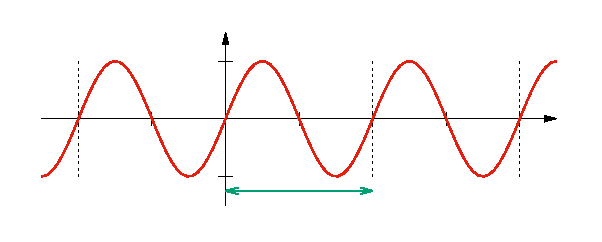
\includegraphics[width={273.60bp},height={100.70bp}]{figura_01_01}}%
    \gplfronttext
  \end{picture}%
\endgroup

    \caption{Función periódica}\label{figura_01}
\end{figure}

Una función periódica es aquella cuya gráfica se repite infinitas veces, cada
cierto intervalo (\textbf{Figura~\ref{figura_01}}).

El menor intervalo de repetición se llama \emph{periodo} ($T$).

Matemáticamente una función periódica es aquella que verifica:
\begin{equation}
    f(t)=f(t+nT);n\in\mathbb{Z}
\label{funcion_periodica}
\end{equation}

Donde $T$ es el periodo (la menor constante que verifica la igualdad).

\section{Propiedades de la funciones periódicas}
Si $f(t)=f(t+nT)$:
\subsection*{Propiedad 1}
\begin{equation}
    \int_a^b\,f(t)\,dt=\int_{a+nT}^{b+nT}f(t)\,dt\quad\,n\in\mathbb{Z}
\label{propiedad1}
\end{equation}

\underline{Prueba}:
\begin{equation*}
    \int_a^b\,f(t)\,dt=\int_{a}^{b}\,f(t+nT)\,dt
\end{equation*}

Cambiando la variable:
\begin{equation*}
    \tau=t+nT
\end{equation*}
\begin{equation*}
    d\tau=dt
\end{equation*}
\begin{equation*}
\begin{split}
    \int_a^b\,f(t)\,dt
        &=\int_{a+nT}^{b+nT}\,f(\tau)\,d\tau\\
        &=\int_{a+nT}^{b+nT}\,f(t)\,dt
\end{split}
\end{equation*}

Puede verse gráficamente en la \textbf{Figura~\ref{figura_02}}.
\begin{figure}[H]
    \centering
    % GNUPLOT: LaTeX picture with Postscript
\begingroup
  \makeatletter
  \providecommand\color[2][]{%
    \GenericError{(gnuplot) \space\space\space\@spaces}{%
      Package color not loaded in conjunction with
      terminal option `colourtext'%
    }{See the gnuplot documentation for explanation.%
    }{Either use 'blacktext' in gnuplot or load the package
      color.sty in LaTeX.}%
    \renewcommand\color[2][]{}%
  }%
  \providecommand\includegraphics[2][]{%
    \GenericError{(gnuplot) \space\space\space\@spaces}{%
      Package graphicx or graphics not loaded%
    }{See the gnuplot documentation for explanation.%
    }{The gnuplot epslatex terminal needs graphicx.sty or graphics.sty.}%
    \renewcommand\includegraphics[2][]{}%
  }%
  \providecommand\rotatebox[2]{#2}%
  \@ifundefined{ifGPcolor}{%
    \newif\ifGPcolor
    \GPcolorfalse
  }{}%
  \@ifundefined{ifGPblacktext}{%
    \newif\ifGPblacktext
    \GPblacktexttrue
  }{}%
  % define a \g@addto@macro without @ in the name:
  \let\gplgaddtomacro\g@addto@macro
  % define empty templates for all commands taking text:
  \gdef\gplbacktext{}%
  \gdef\gplfronttext{}%
  \makeatother
  \ifGPblacktext
    % no textcolor at all
    \def\colorrgb#1{}%
    \def\colorgray#1{}%
  \else
    % gray or color?
    \ifGPcolor
      \def\colorrgb#1{\color[rgb]{#1}}%
      \def\colorgray#1{\color[gray]{#1}}%
      \expandafter\def\csname LTw\endcsname{\color{white}}%
      \expandafter\def\csname LTb\endcsname{\color{black}}%
      \expandafter\def\csname LTa\endcsname{\color{black}}%
      \expandafter\def\csname LT0\endcsname{\color[rgb]{1,0,0}}%
      \expandafter\def\csname LT1\endcsname{\color[rgb]{0,1,0}}%
      \expandafter\def\csname LT2\endcsname{\color[rgb]{0,0,1}}%
      \expandafter\def\csname LT3\endcsname{\color[rgb]{1,0,1}}%
      \expandafter\def\csname LT4\endcsname{\color[rgb]{0,1,1}}%
      \expandafter\def\csname LT5\endcsname{\color[rgb]{1,1,0}}%
      \expandafter\def\csname LT6\endcsname{\color[rgb]{0,0,0}}%
      \expandafter\def\csname LT7\endcsname{\color[rgb]{1,0.3,0}}%
      \expandafter\def\csname LT8\endcsname{\color[rgb]{0.5,0.5,0.5}}%
    \else
      % gray
      \def\colorrgb#1{\color{black}}%
      \def\colorgray#1{\color[gray]{#1}}%
      \expandafter\def\csname LTw\endcsname{\color{white}}%
      \expandafter\def\csname LTb\endcsname{\color{black}}%
      \expandafter\def\csname LTa\endcsname{\color{black}}%
      \expandafter\def\csname LT0\endcsname{\color{black}}%
      \expandafter\def\csname LT1\endcsname{\color{black}}%
      \expandafter\def\csname LT2\endcsname{\color{black}}%
      \expandafter\def\csname LT3\endcsname{\color{black}}%
      \expandafter\def\csname LT4\endcsname{\color{black}}%
      \expandafter\def\csname LT5\endcsname{\color{black}}%
      \expandafter\def\csname LT6\endcsname{\color{black}}%
      \expandafter\def\csname LT7\endcsname{\color{black}}%
      \expandafter\def\csname LT8\endcsname{\color{black}}%
    \fi
  \fi
    \setlength{\unitlength}{0.0500bp}%
    \ifx\gptboxheight\undefined%
      \newlength{\gptboxheight}%
      \newlength{\gptboxwidth}%
      \newsavebox{\gptboxtext}%
    \fi%
    \setlength{\fboxrule}{0.5pt}%
    \setlength{\fboxsep}{1pt}%
    \definecolor{tbcol}{rgb}{1,1,1}%
\begin{picture}(6336.00,2590.00)%
    \gplgaddtomacro\gplbacktext{%
      \csname LTb\endcsname%%
      \put(1233,416){\makebox(0,0)[r]{\strut{}}}%
      \put(1233,863){\makebox(0,0)[r]{\strut{}}}%
      \put(1233,1311){\makebox(0,0)[r]{\strut{}}}%
      \put(1233,1758){\makebox(0,0)[r]{\strut{}}}%
      \put(1233,2205){\makebox(0,0)[r]{\strut{}}}%
      \put(603,640){\makebox(0,0){\strut{}}}%
      \put(1329,640){\makebox(0,0){\strut{}}}%
      \put(2055,640){\makebox(0,0){\strut{}}}%
      \put(2781,640){\makebox(0,0){\strut{}}}%
      \put(3506,640){\makebox(0,0){\strut{}}}%
      \put(4232,640){\makebox(0,0){\strut{}}}%
      \put(4958,640){\makebox(0,0){\strut{}}}%
      \put(5684,640){\makebox(0,0){\strut{}}}%
      \csname LTb\endcsname%%
      \put(6228,863){\makebox(0,0)[l]{\strut{}$t$}}%
      \put(1502,2429){\makebox(0,0)[l]{\strut{}$f(t)$}}%
      \put(2020,662){\makebox(0,0)[l]{\strut{}$a$}}%
      \put(2746,662){\makebox(0,0)[l]{\strut{}$b$}}%
      \put(3955,662){\makebox(0,0)[l]{\strut{}$a+T$}}%
      \put(4704,662){\makebox(0,0)[l]{\strut{}$b+T$}}%
      \put(1766,1982){\makebox(0,0)[l]{\strut{}$\int_a^b f(t) dt$}}%
      \put(3943,2295){\makebox(0,0)[l]{\strut{}$\int_{a+T}^{b+T} f(t+T) dt$}}%
    }%
    \gplgaddtomacro\gplfronttext{%
    }%
    \gplgaddtomacro\gplbacktext{%
      \csname LTb\endcsname%%
      \put(1233,416){\makebox(0,0)[r]{\strut{}}}%
      \put(1233,863){\makebox(0,0)[r]{\strut{}}}%
      \put(1233,1311){\makebox(0,0)[r]{\strut{}}}%
      \put(1233,1758){\makebox(0,0)[r]{\strut{}}}%
      \put(1233,2205){\makebox(0,0)[r]{\strut{}}}%
      \put(603,640){\makebox(0,0){\strut{}}}%
      \put(1329,640){\makebox(0,0){\strut{}}}%
      \put(2055,640){\makebox(0,0){\strut{}}}%
      \put(2781,640){\makebox(0,0){\strut{}}}%
      \put(3506,640){\makebox(0,0){\strut{}}}%
      \put(4232,640){\makebox(0,0){\strut{}}}%
      \put(4958,640){\makebox(0,0){\strut{}}}%
      \put(5684,640){\makebox(0,0){\strut{}}}%
      \csname LTb\endcsname%%
      \put(6228,863){\makebox(0,0)[l]{\strut{}$t$}}%
      \put(1502,2429){\makebox(0,0)[l]{\strut{}$f(t)$}}%
      \put(2020,662){\makebox(0,0)[l]{\strut{}$a$}}%
      \put(2746,662){\makebox(0,0)[l]{\strut{}$b$}}%
      \put(3955,662){\makebox(0,0)[l]{\strut{}$a+T$}}%
      \put(4704,662){\makebox(0,0)[l]{\strut{}$b+T$}}%
      \put(1766,1982){\makebox(0,0)[l]{\strut{}$\int_a^b f(t) dt$}}%
      \put(3943,2295){\makebox(0,0)[l]{\strut{}$\int_{a+T}^{b+T} f(t+T) dt$}}%
    }%
    \gplgaddtomacro\gplfronttext{%
    }%
    \gplgaddtomacro\gplbacktext{%
      \csname LTb\endcsname%%
      \put(1233,416){\makebox(0,0)[r]{\strut{}}}%
      \put(1233,863){\makebox(0,0)[r]{\strut{}}}%
      \put(1233,1311){\makebox(0,0)[r]{\strut{}}}%
      \put(1233,1758){\makebox(0,0)[r]{\strut{}}}%
      \put(1233,2205){\makebox(0,0)[r]{\strut{}}}%
      \put(603,640){\makebox(0,0){\strut{}}}%
      \put(1329,640){\makebox(0,0){\strut{}}}%
      \put(2055,640){\makebox(0,0){\strut{}}}%
      \put(2781,640){\makebox(0,0){\strut{}}}%
      \put(3506,640){\makebox(0,0){\strut{}}}%
      \put(4232,640){\makebox(0,0){\strut{}}}%
      \put(4958,640){\makebox(0,0){\strut{}}}%
      \put(5684,640){\makebox(0,0){\strut{}}}%
      \csname LTb\endcsname%%
      \put(6228,863){\makebox(0,0)[l]{\strut{}$t$}}%
      \put(1502,2429){\makebox(0,0)[l]{\strut{}$f(t)$}}%
      \put(2020,662){\makebox(0,0)[l]{\strut{}$a$}}%
      \put(2746,662){\makebox(0,0)[l]{\strut{}$b$}}%
      \put(3955,662){\makebox(0,0)[l]{\strut{}$a+T$}}%
      \put(4704,662){\makebox(0,0)[l]{\strut{}$b+T$}}%
      \put(1766,1982){\makebox(0,0)[l]{\strut{}$\int_a^b f(t) dt$}}%
      \put(3943,2295){\makebox(0,0)[l]{\strut{}$\int_{a+T}^{b+T} f(t+T) dt$}}%
    }%
    \gplgaddtomacro\gplfronttext{%
    }%
    \gplgaddtomacro\gplbacktext{%
      \csname LTb\endcsname%%
      \put(1233,416){\makebox(0,0)[r]{\strut{}}}%
      \put(1233,863){\makebox(0,0)[r]{\strut{}}}%
      \put(1233,1311){\makebox(0,0)[r]{\strut{}}}%
      \put(1233,1758){\makebox(0,0)[r]{\strut{}}}%
      \put(1233,2205){\makebox(0,0)[r]{\strut{}}}%
      \put(603,640){\makebox(0,0){\strut{}}}%
      \put(1329,640){\makebox(0,0){\strut{}}}%
      \put(2055,640){\makebox(0,0){\strut{}}}%
      \put(2781,640){\makebox(0,0){\strut{}}}%
      \put(3506,640){\makebox(0,0){\strut{}}}%
      \put(4232,640){\makebox(0,0){\strut{}}}%
      \put(4958,640){\makebox(0,0){\strut{}}}%
      \put(5684,640){\makebox(0,0){\strut{}}}%
      \csname LTb\endcsname%%
      \put(6228,863){\makebox(0,0)[l]{\strut{}$t$}}%
      \put(1502,2429){\makebox(0,0)[l]{\strut{}$f(t)$}}%
      \put(2020,662){\makebox(0,0)[l]{\strut{}$a$}}%
      \put(2746,662){\makebox(0,0)[l]{\strut{}$b$}}%
      \put(3955,662){\makebox(0,0)[l]{\strut{}$a+T$}}%
      \put(4704,662){\makebox(0,0)[l]{\strut{}$b+T$}}%
      \put(1766,1982){\makebox(0,0)[l]{\strut{}$\int_a^b f(t) dt$}}%
      \put(3943,2295){\makebox(0,0)[l]{\strut{}$\int_{a+T}^{b+T} f(t+T) dt$}}%
    }%
    \gplgaddtomacro\gplfronttext{%
    }%
    \gplgaddtomacro\gplbacktext{%
      \csname LTb\endcsname%%
      \put(1233,416){\makebox(0,0)[r]{\strut{}}}%
      \put(1233,863){\makebox(0,0)[r]{\strut{}}}%
      \put(1233,1311){\makebox(0,0)[r]{\strut{}}}%
      \put(1233,1758){\makebox(0,0)[r]{\strut{}}}%
      \put(1233,2205){\makebox(0,0)[r]{\strut{}}}%
      \put(603,640){\makebox(0,0){\strut{}}}%
      \put(1329,640){\makebox(0,0){\strut{}}}%
      \put(2055,640){\makebox(0,0){\strut{}}}%
      \put(2781,640){\makebox(0,0){\strut{}}}%
      \put(3506,640){\makebox(0,0){\strut{}}}%
      \put(4232,640){\makebox(0,0){\strut{}}}%
      \put(4958,640){\makebox(0,0){\strut{}}}%
      \put(5684,640){\makebox(0,0){\strut{}}}%
      \csname LTb\endcsname%%
      \put(6228,863){\makebox(0,0)[l]{\strut{}$t$}}%
      \put(1502,2429){\makebox(0,0)[l]{\strut{}$f(t)$}}%
      \put(2020,662){\makebox(0,0)[l]{\strut{}$a$}}%
      \put(2746,662){\makebox(0,0)[l]{\strut{}$b$}}%
      \put(3955,662){\makebox(0,0)[l]{\strut{}$a+T$}}%
      \put(4704,662){\makebox(0,0)[l]{\strut{}$b+T$}}%
      \put(1766,1982){\makebox(0,0)[l]{\strut{}$\int_a^b f(t) dt$}}%
      \put(3943,2295){\makebox(0,0)[l]{\strut{}$\int_{a+T}^{b+T} f(t+T) dt$}}%
    }%
    \gplgaddtomacro\gplfronttext{%
    }%
    \gplgaddtomacro\gplbacktext{%
      \csname LTb\endcsname%%
      \put(1233,416){\makebox(0,0)[r]{\strut{}}}%
      \put(1233,863){\makebox(0,0)[r]{\strut{}}}%
      \put(1233,1311){\makebox(0,0)[r]{\strut{}}}%
      \put(1233,1758){\makebox(0,0)[r]{\strut{}}}%
      \put(1233,2205){\makebox(0,0)[r]{\strut{}}}%
      \put(603,640){\makebox(0,0){\strut{}}}%
      \put(1329,640){\makebox(0,0){\strut{}}}%
      \put(2055,640){\makebox(0,0){\strut{}}}%
      \put(2781,640){\makebox(0,0){\strut{}}}%
      \put(3506,640){\makebox(0,0){\strut{}}}%
      \put(4232,640){\makebox(0,0){\strut{}}}%
      \put(4958,640){\makebox(0,0){\strut{}}}%
      \put(5684,640){\makebox(0,0){\strut{}}}%
      \csname LTb\endcsname%%
      \put(6228,863){\makebox(0,0)[l]{\strut{}$t$}}%
      \put(1502,2429){\makebox(0,0)[l]{\strut{}$f(t)$}}%
      \put(2020,662){\makebox(0,0)[l]{\strut{}$a$}}%
      \put(2746,662){\makebox(0,0)[l]{\strut{}$b$}}%
      \put(3955,662){\makebox(0,0)[l]{\strut{}$a+T$}}%
      \put(4704,662){\makebox(0,0)[l]{\strut{}$b+T$}}%
      \put(1766,1982){\makebox(0,0)[l]{\strut{}$\int_a^b f(t) dt$}}%
      \put(3943,2295){\makebox(0,0)[l]{\strut{}$\int_{a+T}^{b+T} f(t+T) dt$}}%
    }%
    \gplgaddtomacro\gplfronttext{%
    }%
    \gplbacktext
    \put(0,0){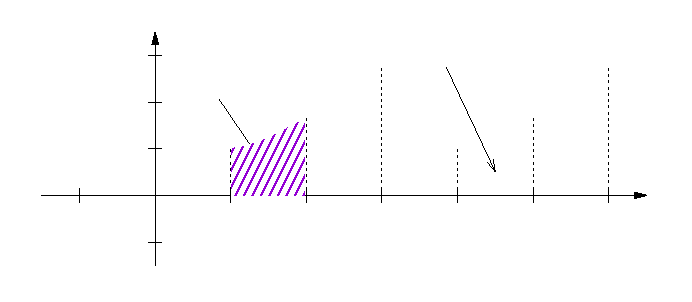
\includegraphics[width={316.80bp},height={129.50bp}]{figura_01_02}}%
    \gplfronttext
  \end{picture}%
\endgroup

    \caption{Demostración gráfica}\label{figura_02}
\end{figure}

\subsection*{Propiedad 2}
\begin{equation}
    \int_{a-T/2}^{a+T/2}f(t)\,dt=\int_{-T/2}^{T/2}f(t)\,dt
\label{propiedad2}
\end{equation}

\underline{Prueba}:
\begin{equation*}
\begin{split}
    \int_{a-T/2}^{a+T/2}f(t)\,dt
        &=\int_{a-T/2}^{T/2}f(t)\,dt+\int_{T/2}^{a+T/2}f(t)\,dt\\
        &=\int_{a-T/2}^{T/2}f(t)\,dt+\int_{T/2-T}^{a+T/2-T}f(t)\,dt\\
        &=\int_{a-T/2}^{T/2}f(t)\,dt+\int_{-T/2}^{a-T/2}f(t)\,dt\\
        &=\int_{-T/2}^{T/2}f(t)\,dt
\end{split}
\end{equation*}

Puede verse gráficamente en la \textbf{Figura~\ref{figura_03}}.
\begin{figure}[H]
    \centering
    % GNUPLOT: LaTeX picture with Postscript
\begingroup
  \makeatletter
  \providecommand\color[2][]{%
    \GenericError{(gnuplot) \space\space\space\@spaces}{%
      Package color not loaded in conjunction with
      terminal option `colourtext'%
    }{See the gnuplot documentation for explanation.%
    }{Either use 'blacktext' in gnuplot or load the package
      color.sty in LaTeX.}%
    \renewcommand\color[2][]{}%
  }%
  \providecommand\includegraphics[2][]{%
    \GenericError{(gnuplot) \space\space\space\@spaces}{%
      Package graphicx or graphics not loaded%
    }{See the gnuplot documentation for explanation.%
    }{The gnuplot epslatex terminal needs graphicx.sty or graphics.sty.}%
    \renewcommand\includegraphics[2][]{}%
  }%
  \providecommand\rotatebox[2]{#2}%
  \@ifundefined{ifGPcolor}{%
    \newif\ifGPcolor
    \GPcolorfalse
  }{}%
  \@ifundefined{ifGPblacktext}{%
    \newif\ifGPblacktext
    \GPblacktexttrue
  }{}%
  % define a \g@addto@macro without @ in the name:
  \let\gplgaddtomacro\g@addto@macro
  % define empty templates for all commands taking text:
  \gdef\gplbacktext{}%
  \gdef\gplfronttext{}%
  \makeatother
  \ifGPblacktext
    % no textcolor at all
    \def\colorrgb#1{}%
    \def\colorgray#1{}%
  \else
    % gray or color?
    \ifGPcolor
      \def\colorrgb#1{\color[rgb]{#1}}%
      \def\colorgray#1{\color[gray]{#1}}%
      \expandafter\def\csname LTw\endcsname{\color{white}}%
      \expandafter\def\csname LTb\endcsname{\color{black}}%
      \expandafter\def\csname LTa\endcsname{\color{black}}%
      \expandafter\def\csname LT0\endcsname{\color[rgb]{1,0,0}}%
      \expandafter\def\csname LT1\endcsname{\color[rgb]{0,1,0}}%
      \expandafter\def\csname LT2\endcsname{\color[rgb]{0,0,1}}%
      \expandafter\def\csname LT3\endcsname{\color[rgb]{1,0,1}}%
      \expandafter\def\csname LT4\endcsname{\color[rgb]{0,1,1}}%
      \expandafter\def\csname LT5\endcsname{\color[rgb]{1,1,0}}%
      \expandafter\def\csname LT6\endcsname{\color[rgb]{0,0,0}}%
      \expandafter\def\csname LT7\endcsname{\color[rgb]{1,0.3,0}}%
      \expandafter\def\csname LT8\endcsname{\color[rgb]{0.5,0.5,0.5}}%
    \else
      % gray
      \def\colorrgb#1{\color{black}}%
      \def\colorgray#1{\color[gray]{#1}}%
      \expandafter\def\csname LTw\endcsname{\color{white}}%
      \expandafter\def\csname LTb\endcsname{\color{black}}%
      \expandafter\def\csname LTa\endcsname{\color{black}}%
      \expandafter\def\csname LT0\endcsname{\color{black}}%
      \expandafter\def\csname LT1\endcsname{\color{black}}%
      \expandafter\def\csname LT2\endcsname{\color{black}}%
      \expandafter\def\csname LT3\endcsname{\color{black}}%
      \expandafter\def\csname LT4\endcsname{\color{black}}%
      \expandafter\def\csname LT5\endcsname{\color{black}}%
      \expandafter\def\csname LT6\endcsname{\color{black}}%
      \expandafter\def\csname LT7\endcsname{\color{black}}%
      \expandafter\def\csname LT8\endcsname{\color{black}}%
    \fi
  \fi
    \setlength{\unitlength}{0.0500bp}%
    \ifx\gptboxheight\undefined%
      \newlength{\gptboxheight}%
      \newlength{\gptboxwidth}%
      \newsavebox{\gptboxtext}%
    \fi%
    \setlength{\fboxrule}{0.5pt}%
    \setlength{\fboxsep}{1pt}%
    \definecolor{tbcol}{rgb}{1,1,1}%
\begin{picture}(6336.00,2590.00)%
    \gplgaddtomacro\gplbacktext{%
      \csname LTb\endcsname%%
      \put(1757,416){\makebox(0,0)[r]{\strut{}}}%
      \put(1757,863){\makebox(0,0)[r]{\strut{}}}%
      \put(1757,1311){\makebox(0,0)[r]{\strut{}}}%
      \put(1757,1758){\makebox(0,0)[r]{\strut{}}}%
      \put(1757,2205){\makebox(0,0)[r]{\strut{}}}%
      \put(563,640){\makebox(0,0){\strut{}}}%
      \put(1208,640){\makebox(0,0){\strut{}}}%
      \put(1853,640){\makebox(0,0){\strut{}}}%
      \put(2498,640){\makebox(0,0){\strut{}}}%
      \put(3143,640){\makebox(0,0){\strut{}}}%
      \put(3789,640){\makebox(0,0){\strut{}}}%
      \put(4434,640){\makebox(0,0){\strut{}}}%
      \put(5079,640){\makebox(0,0){\strut{}}}%
      \put(5724,640){\makebox(0,0){\strut{}}}%
      \csname LTb\endcsname%%
      \put(6208,863){\makebox(0,0)[l]{\strut{}$t$}}%
      \put(2007,2429){\makebox(0,0)[l]{\strut{}$f(t)$}}%
      \put(631,662){\makebox(0,0)[l]{\strut{}$-\frac{T}{2}$}}%
      \put(2728,662){\makebox(0,0)[l]{\strut{}$\frac{T}{2}$}}%
      \put(3203,662){\makebox(0,0)[l]{\strut{}$a-\frac{T}{2}$}}%
      \put(4383,662){\makebox(0,0)[l]{\strut{}$a$}}%
      \put(5201,662){\makebox(0,0)[l]{\strut{}$a+\frac{T}{2}$}}%
      \put(306,2026){\makebox(0,0)[l]{\strut{}$\int_{-\frac{T}{2}}^{\frac{T}{2}} f(t) dt$}}%
      \put(4177,2295){\makebox(0,0)[l]{\strut{}$\int_{a-\frac{T}{2}}^{a+\frac{T}{2}} f(t) dt$}}%
    }%
    \gplgaddtomacro\gplfronttext{%
    }%
    \gplgaddtomacro\gplbacktext{%
      \csname LTb\endcsname%%
      \put(1757,416){\makebox(0,0)[r]{\strut{}}}%
      \put(1757,863){\makebox(0,0)[r]{\strut{}}}%
      \put(1757,1311){\makebox(0,0)[r]{\strut{}}}%
      \put(1757,1758){\makebox(0,0)[r]{\strut{}}}%
      \put(1757,2205){\makebox(0,0)[r]{\strut{}}}%
      \put(563,640){\makebox(0,0){\strut{}}}%
      \put(1208,640){\makebox(0,0){\strut{}}}%
      \put(1853,640){\makebox(0,0){\strut{}}}%
      \put(2498,640){\makebox(0,0){\strut{}}}%
      \put(3143,640){\makebox(0,0){\strut{}}}%
      \put(3789,640){\makebox(0,0){\strut{}}}%
      \put(4434,640){\makebox(0,0){\strut{}}}%
      \put(5079,640){\makebox(0,0){\strut{}}}%
      \put(5724,640){\makebox(0,0){\strut{}}}%
      \csname LTb\endcsname%%
      \put(6208,863){\makebox(0,0)[l]{\strut{}$t$}}%
      \put(2007,2429){\makebox(0,0)[l]{\strut{}$f(t)$}}%
      \put(631,662){\makebox(0,0)[l]{\strut{}$-\frac{T}{2}$}}%
      \put(2728,662){\makebox(0,0)[l]{\strut{}$\frac{T}{2}$}}%
      \put(3203,662){\makebox(0,0)[l]{\strut{}$a-\frac{T}{2}$}}%
      \put(4383,662){\makebox(0,0)[l]{\strut{}$a$}}%
      \put(5201,662){\makebox(0,0)[l]{\strut{}$a+\frac{T}{2}$}}%
      \put(306,2026){\makebox(0,0)[l]{\strut{}$\int_{-\frac{T}{2}}^{\frac{T}{2}} f(t) dt$}}%
      \put(4177,2295){\makebox(0,0)[l]{\strut{}$\int_{a-\frac{T}{2}}^{a+\frac{T}{2}} f(t) dt$}}%
    }%
    \gplgaddtomacro\gplfronttext{%
    }%
    \gplgaddtomacro\gplbacktext{%
      \csname LTb\endcsname%%
      \put(1757,416){\makebox(0,0)[r]{\strut{}}}%
      \put(1757,863){\makebox(0,0)[r]{\strut{}}}%
      \put(1757,1311){\makebox(0,0)[r]{\strut{}}}%
      \put(1757,1758){\makebox(0,0)[r]{\strut{}}}%
      \put(1757,2205){\makebox(0,0)[r]{\strut{}}}%
      \put(563,640){\makebox(0,0){\strut{}}}%
      \put(1208,640){\makebox(0,0){\strut{}}}%
      \put(1853,640){\makebox(0,0){\strut{}}}%
      \put(2498,640){\makebox(0,0){\strut{}}}%
      \put(3143,640){\makebox(0,0){\strut{}}}%
      \put(3789,640){\makebox(0,0){\strut{}}}%
      \put(4434,640){\makebox(0,0){\strut{}}}%
      \put(5079,640){\makebox(0,0){\strut{}}}%
      \put(5724,640){\makebox(0,0){\strut{}}}%
      \csname LTb\endcsname%%
      \put(6208,863){\makebox(0,0)[l]{\strut{}$t$}}%
      \put(2007,2429){\makebox(0,0)[l]{\strut{}$f(t)$}}%
      \put(631,662){\makebox(0,0)[l]{\strut{}$-\frac{T}{2}$}}%
      \put(2728,662){\makebox(0,0)[l]{\strut{}$\frac{T}{2}$}}%
      \put(3203,662){\makebox(0,0)[l]{\strut{}$a-\frac{T}{2}$}}%
      \put(4383,662){\makebox(0,0)[l]{\strut{}$a$}}%
      \put(5201,662){\makebox(0,0)[l]{\strut{}$a+\frac{T}{2}$}}%
      \put(306,2026){\makebox(0,0)[l]{\strut{}$\int_{-\frac{T}{2}}^{\frac{T}{2}} f(t) dt$}}%
      \put(4177,2295){\makebox(0,0)[l]{\strut{}$\int_{a-\frac{T}{2}}^{a+\frac{T}{2}} f(t) dt$}}%
    }%
    \gplgaddtomacro\gplfronttext{%
    }%
    \gplgaddtomacro\gplbacktext{%
      \csname LTb\endcsname%%
      \put(1757,416){\makebox(0,0)[r]{\strut{}}}%
      \put(1757,863){\makebox(0,0)[r]{\strut{}}}%
      \put(1757,1311){\makebox(0,0)[r]{\strut{}}}%
      \put(1757,1758){\makebox(0,0)[r]{\strut{}}}%
      \put(1757,2205){\makebox(0,0)[r]{\strut{}}}%
      \put(563,640){\makebox(0,0){\strut{}}}%
      \put(1208,640){\makebox(0,0){\strut{}}}%
      \put(1853,640){\makebox(0,0){\strut{}}}%
      \put(2498,640){\makebox(0,0){\strut{}}}%
      \put(3143,640){\makebox(0,0){\strut{}}}%
      \put(3789,640){\makebox(0,0){\strut{}}}%
      \put(4434,640){\makebox(0,0){\strut{}}}%
      \put(5079,640){\makebox(0,0){\strut{}}}%
      \put(5724,640){\makebox(0,0){\strut{}}}%
      \csname LTb\endcsname%%
      \put(6208,863){\makebox(0,0)[l]{\strut{}$t$}}%
      \put(2007,2429){\makebox(0,0)[l]{\strut{}$f(t)$}}%
      \put(631,662){\makebox(0,0)[l]{\strut{}$-\frac{T}{2}$}}%
      \put(2728,662){\makebox(0,0)[l]{\strut{}$\frac{T}{2}$}}%
      \put(3203,662){\makebox(0,0)[l]{\strut{}$a-\frac{T}{2}$}}%
      \put(4383,662){\makebox(0,0)[l]{\strut{}$a$}}%
      \put(5201,662){\makebox(0,0)[l]{\strut{}$a+\frac{T}{2}$}}%
      \put(306,2026){\makebox(0,0)[l]{\strut{}$\int_{-\frac{T}{2}}^{\frac{T}{2}} f(t) dt$}}%
      \put(4177,2295){\makebox(0,0)[l]{\strut{}$\int_{a-\frac{T}{2}}^{a+\frac{T}{2}} f(t) dt$}}%
    }%
    \gplgaddtomacro\gplfronttext{%
    }%
    \gplgaddtomacro\gplbacktext{%
      \csname LTb\endcsname%%
      \put(1757,416){\makebox(0,0)[r]{\strut{}}}%
      \put(1757,863){\makebox(0,0)[r]{\strut{}}}%
      \put(1757,1311){\makebox(0,0)[r]{\strut{}}}%
      \put(1757,1758){\makebox(0,0)[r]{\strut{}}}%
      \put(1757,2205){\makebox(0,0)[r]{\strut{}}}%
      \put(563,640){\makebox(0,0){\strut{}}}%
      \put(1208,640){\makebox(0,0){\strut{}}}%
      \put(1853,640){\makebox(0,0){\strut{}}}%
      \put(2498,640){\makebox(0,0){\strut{}}}%
      \put(3143,640){\makebox(0,0){\strut{}}}%
      \put(3789,640){\makebox(0,0){\strut{}}}%
      \put(4434,640){\makebox(0,0){\strut{}}}%
      \put(5079,640){\makebox(0,0){\strut{}}}%
      \put(5724,640){\makebox(0,0){\strut{}}}%
      \csname LTb\endcsname%%
      \put(6208,863){\makebox(0,0)[l]{\strut{}$t$}}%
      \put(2007,2429){\makebox(0,0)[l]{\strut{}$f(t)$}}%
      \put(631,662){\makebox(0,0)[l]{\strut{}$-\frac{T}{2}$}}%
      \put(2728,662){\makebox(0,0)[l]{\strut{}$\frac{T}{2}$}}%
      \put(3203,662){\makebox(0,0)[l]{\strut{}$a-\frac{T}{2}$}}%
      \put(4383,662){\makebox(0,0)[l]{\strut{}$a$}}%
      \put(5201,662){\makebox(0,0)[l]{\strut{}$a+\frac{T}{2}$}}%
      \put(306,2026){\makebox(0,0)[l]{\strut{}$\int_{-\frac{T}{2}}^{\frac{T}{2}} f(t) dt$}}%
      \put(4177,2295){\makebox(0,0)[l]{\strut{}$\int_{a-\frac{T}{2}}^{a+\frac{T}{2}} f(t) dt$}}%
    }%
    \gplgaddtomacro\gplfronttext{%
    }%
    \gplgaddtomacro\gplbacktext{%
      \csname LTb\endcsname%%
      \put(1757,416){\makebox(0,0)[r]{\strut{}}}%
      \put(1757,863){\makebox(0,0)[r]{\strut{}}}%
      \put(1757,1311){\makebox(0,0)[r]{\strut{}}}%
      \put(1757,1758){\makebox(0,0)[r]{\strut{}}}%
      \put(1757,2205){\makebox(0,0)[r]{\strut{}}}%
      \put(563,640){\makebox(0,0){\strut{}}}%
      \put(1208,640){\makebox(0,0){\strut{}}}%
      \put(1853,640){\makebox(0,0){\strut{}}}%
      \put(2498,640){\makebox(0,0){\strut{}}}%
      \put(3143,640){\makebox(0,0){\strut{}}}%
      \put(3789,640){\makebox(0,0){\strut{}}}%
      \put(4434,640){\makebox(0,0){\strut{}}}%
      \put(5079,640){\makebox(0,0){\strut{}}}%
      \put(5724,640){\makebox(0,0){\strut{}}}%
      \csname LTb\endcsname%%
      \put(6208,863){\makebox(0,0)[l]{\strut{}$t$}}%
      \put(2007,2429){\makebox(0,0)[l]{\strut{}$f(t)$}}%
      \put(631,662){\makebox(0,0)[l]{\strut{}$-\frac{T}{2}$}}%
      \put(2728,662){\makebox(0,0)[l]{\strut{}$\frac{T}{2}$}}%
      \put(3203,662){\makebox(0,0)[l]{\strut{}$a-\frac{T}{2}$}}%
      \put(4383,662){\makebox(0,0)[l]{\strut{}$a$}}%
      \put(5201,662){\makebox(0,0)[l]{\strut{}$a+\frac{T}{2}$}}%
      \put(306,2026){\makebox(0,0)[l]{\strut{}$\int_{-\frac{T}{2}}^{\frac{T}{2}} f(t) dt$}}%
      \put(4177,2295){\makebox(0,0)[l]{\strut{}$\int_{a-\frac{T}{2}}^{a+\frac{T}{2}} f(t) dt$}}%
    }%
    \gplgaddtomacro\gplfronttext{%
    }%
    \gplgaddtomacro\gplbacktext{%
      \csname LTb\endcsname%%
      \put(1757,416){\makebox(0,0)[r]{\strut{}}}%
      \put(1757,863){\makebox(0,0)[r]{\strut{}}}%
      \put(1757,1311){\makebox(0,0)[r]{\strut{}}}%
      \put(1757,1758){\makebox(0,0)[r]{\strut{}}}%
      \put(1757,2205){\makebox(0,0)[r]{\strut{}}}%
      \put(563,640){\makebox(0,0){\strut{}}}%
      \put(1208,640){\makebox(0,0){\strut{}}}%
      \put(1853,640){\makebox(0,0){\strut{}}}%
      \put(2498,640){\makebox(0,0){\strut{}}}%
      \put(3143,640){\makebox(0,0){\strut{}}}%
      \put(3789,640){\makebox(0,0){\strut{}}}%
      \put(4434,640){\makebox(0,0){\strut{}}}%
      \put(5079,640){\makebox(0,0){\strut{}}}%
      \put(5724,640){\makebox(0,0){\strut{}}}%
      \csname LTb\endcsname%%
      \put(6208,863){\makebox(0,0)[l]{\strut{}$t$}}%
      \put(2007,2429){\makebox(0,0)[l]{\strut{}$f(t)$}}%
      \put(631,662){\makebox(0,0)[l]{\strut{}$-\frac{T}{2}$}}%
      \put(2728,662){\makebox(0,0)[l]{\strut{}$\frac{T}{2}$}}%
      \put(3203,662){\makebox(0,0)[l]{\strut{}$a-\frac{T}{2}$}}%
      \put(4383,662){\makebox(0,0)[l]{\strut{}$a$}}%
      \put(5201,662){\makebox(0,0)[l]{\strut{}$a+\frac{T}{2}$}}%
      \put(306,2026){\makebox(0,0)[l]{\strut{}$\int_{-\frac{T}{2}}^{\frac{T}{2}} f(t) dt$}}%
      \put(4177,2295){\makebox(0,0)[l]{\strut{}$\int_{a-\frac{T}{2}}^{a+\frac{T}{2}} f(t) dt$}}%
    }%
    \gplgaddtomacro\gplfronttext{%
    }%
    \gplgaddtomacro\gplbacktext{%
      \csname LTb\endcsname%%
      \put(1757,416){\makebox(0,0)[r]{\strut{}}}%
      \put(1757,863){\makebox(0,0)[r]{\strut{}}}%
      \put(1757,1311){\makebox(0,0)[r]{\strut{}}}%
      \put(1757,1758){\makebox(0,0)[r]{\strut{}}}%
      \put(1757,2205){\makebox(0,0)[r]{\strut{}}}%
      \put(563,640){\makebox(0,0){\strut{}}}%
      \put(1208,640){\makebox(0,0){\strut{}}}%
      \put(1853,640){\makebox(0,0){\strut{}}}%
      \put(2498,640){\makebox(0,0){\strut{}}}%
      \put(3143,640){\makebox(0,0){\strut{}}}%
      \put(3789,640){\makebox(0,0){\strut{}}}%
      \put(4434,640){\makebox(0,0){\strut{}}}%
      \put(5079,640){\makebox(0,0){\strut{}}}%
      \put(5724,640){\makebox(0,0){\strut{}}}%
      \csname LTb\endcsname%%
      \put(6208,863){\makebox(0,0)[l]{\strut{}$t$}}%
      \put(2007,2429){\makebox(0,0)[l]{\strut{}$f(t)$}}%
      \put(631,662){\makebox(0,0)[l]{\strut{}$-\frac{T}{2}$}}%
      \put(2728,662){\makebox(0,0)[l]{\strut{}$\frac{T}{2}$}}%
      \put(3203,662){\makebox(0,0)[l]{\strut{}$a-\frac{T}{2}$}}%
      \put(4383,662){\makebox(0,0)[l]{\strut{}$a$}}%
      \put(5201,662){\makebox(0,0)[l]{\strut{}$a+\frac{T}{2}$}}%
      \put(306,2026){\makebox(0,0)[l]{\strut{}$\int_{-\frac{T}{2}}^{\frac{T}{2}} f(t) dt$}}%
      \put(4177,2295){\makebox(0,0)[l]{\strut{}$\int_{a-\frac{T}{2}}^{a+\frac{T}{2}} f(t) dt$}}%
    }%
    \gplgaddtomacro\gplfronttext{%
    }%
    \gplbacktext
    \put(0,0){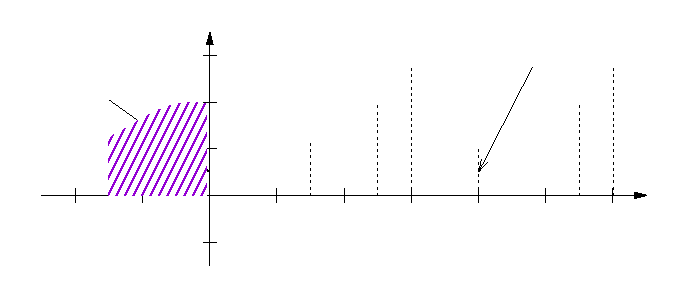
\includegraphics[width={316.80bp},height={129.50bp}]{figura_01_03}}%
    \gplfronttext
  \end{picture}%
\endgroup

    \caption{Demostración gráfica}\label{figura_03}
\end{figure}

\subsection*{Propiedad 3}
\begin{equation}
    \int_{0}^{T}f(t)\,dt=\int_{-T/2}^{T/2}f(t)\,dt
\label{propiedad3}
\end{equation}

\underline{Prueba}:

Si en la ecuación (\ref{propiedad2}) $a=T/2$:
\begin{equation*}
\begin{split}
    \int_{-T/2}^{T/2}f(t)\,dt
        &=\int_{a-T/2}^{a+T/2}f(t)\,dt\\
        &=\int_{T/2-T/2}^{T/2+T/2}f(t)\,dt\\
        &=\int_{0}^{T}f(t)\,dt
\end{split}
\end{equation*}

Puede verse gráficamente en la \textbf{Figura~\ref{figura_04}}.
\begin{figure}[H]
    \centering
    % GNUPLOT: LaTeX picture with Postscript
\begingroup
  \makeatletter
  \providecommand\color[2][]{%
    \GenericError{(gnuplot) \space\space\space\@spaces}{%
      Package color not loaded in conjunction with
      terminal option `colourtext'%
    }{See the gnuplot documentation for explanation.%
    }{Either use 'blacktext' in gnuplot or load the package
      color.sty in LaTeX.}%
    \renewcommand\color[2][]{}%
  }%
  \providecommand\includegraphics[2][]{%
    \GenericError{(gnuplot) \space\space\space\@spaces}{%
      Package graphicx or graphics not loaded%
    }{See the gnuplot documentation for explanation.%
    }{The gnuplot epslatex terminal needs graphicx.sty or graphics.sty.}%
    \renewcommand\includegraphics[2][]{}%
  }%
  \providecommand\rotatebox[2]{#2}%
  \@ifundefined{ifGPcolor}{%
    \newif\ifGPcolor
    \GPcolorfalse
  }{}%
  \@ifundefined{ifGPblacktext}{%
    \newif\ifGPblacktext
    \GPblacktexttrue
  }{}%
  % define a \g@addto@macro without @ in the name:
  \let\gplgaddtomacro\g@addto@macro
  % define empty templates for all commands taking text:
  \gdef\gplbacktext{}%
  \gdef\gplfronttext{}%
  \makeatother
  \ifGPblacktext
    % no textcolor at all
    \def\colorrgb#1{}%
    \def\colorgray#1{}%
  \else
    % gray or color?
    \ifGPcolor
      \def\colorrgb#1{\color[rgb]{#1}}%
      \def\colorgray#1{\color[gray]{#1}}%
      \expandafter\def\csname LTw\endcsname{\color{white}}%
      \expandafter\def\csname LTb\endcsname{\color{black}}%
      \expandafter\def\csname LTa\endcsname{\color{black}}%
      \expandafter\def\csname LT0\endcsname{\color[rgb]{1,0,0}}%
      \expandafter\def\csname LT1\endcsname{\color[rgb]{0,1,0}}%
      \expandafter\def\csname LT2\endcsname{\color[rgb]{0,0,1}}%
      \expandafter\def\csname LT3\endcsname{\color[rgb]{1,0,1}}%
      \expandafter\def\csname LT4\endcsname{\color[rgb]{0,1,1}}%
      \expandafter\def\csname LT5\endcsname{\color[rgb]{1,1,0}}%
      \expandafter\def\csname LT6\endcsname{\color[rgb]{0,0,0}}%
      \expandafter\def\csname LT7\endcsname{\color[rgb]{1,0.3,0}}%
      \expandafter\def\csname LT8\endcsname{\color[rgb]{0.5,0.5,0.5}}%
    \else
      % gray
      \def\colorrgb#1{\color{black}}%
      \def\colorgray#1{\color[gray]{#1}}%
      \expandafter\def\csname LTw\endcsname{\color{white}}%
      \expandafter\def\csname LTb\endcsname{\color{black}}%
      \expandafter\def\csname LTa\endcsname{\color{black}}%
      \expandafter\def\csname LT0\endcsname{\color{black}}%
      \expandafter\def\csname LT1\endcsname{\color{black}}%
      \expandafter\def\csname LT2\endcsname{\color{black}}%
      \expandafter\def\csname LT3\endcsname{\color{black}}%
      \expandafter\def\csname LT4\endcsname{\color{black}}%
      \expandafter\def\csname LT5\endcsname{\color{black}}%
      \expandafter\def\csname LT6\endcsname{\color{black}}%
      \expandafter\def\csname LT7\endcsname{\color{black}}%
      \expandafter\def\csname LT8\endcsname{\color{black}}%
    \fi
  \fi
    \setlength{\unitlength}{0.0500bp}%
    \ifx\gptboxheight\undefined%
      \newlength{\gptboxheight}%
      \newlength{\gptboxwidth}%
      \newsavebox{\gptboxtext}%
    \fi%
    \setlength{\fboxrule}{0.5pt}%
    \setlength{\fboxsep}{1pt}%
    \definecolor{tbcol}{rgb}{1,1,1}%
\begin{picture}(6336.00,2590.00)%
    \gplgaddtomacro\gplbacktext{%
      \csname LTb\endcsname%%
      \put(2356,455){\makebox(0,0)[r]{\strut{}}}%
      \put(2356,982){\makebox(0,0)[r]{\strut{}}}%
      \put(2356,1508){\makebox(0,0)[r]{\strut{}}}%
      \put(2356,2034){\makebox(0,0)[r]{\strut{}}}%
      \put(240,759){\makebox(0,0){\strut{}}}%
      \put(1346,759){\makebox(0,0){\strut{}}}%
      \put(2452,759){\makebox(0,0){\strut{}}}%
      \put(3558,759){\makebox(0,0){\strut{}}}%
      \put(4664,759){\makebox(0,0){\strut{}}}%
      \put(5770,759){\makebox(0,0){\strut{}}}%
      \csname LTb\endcsname%%
      \put(6324,982){\makebox(0,0)[l]{\strut{}$t$}}%
      \put(2628,2561){\makebox(0,0)[l]{\strut{}$f(t)$}}%
      \put(574,745){\makebox(0,0)[l]{\strut{}$-\frac{T}{2}$}}%
      \put(4059,745){\makebox(0,0)[l]{\strut{}$ \frac{T}{2}$}}%
      \put(5735,745){\makebox(0,0)[l]{\strut{}$T$}}%
      \put(265,2350){\makebox(0,0)[l]{\strut{}$\int_{-\frac{T}{2}}^{\frac{T}{2}} f(t) dt$}}%
      \put(3231,2350){\makebox(0,0)[l]{\strut{}$\int_{0}^{T} f(t) dt$}}%
    }%
    \gplgaddtomacro\gplfronttext{%
    }%
    \gplgaddtomacro\gplbacktext{%
      \csname LTb\endcsname%%
      \put(2356,455){\makebox(0,0)[r]{\strut{}}}%
      \put(2356,982){\makebox(0,0)[r]{\strut{}}}%
      \put(2356,1508){\makebox(0,0)[r]{\strut{}}}%
      \put(2356,2034){\makebox(0,0)[r]{\strut{}}}%
      \put(240,759){\makebox(0,0){\strut{}}}%
      \put(1346,759){\makebox(0,0){\strut{}}}%
      \put(2452,759){\makebox(0,0){\strut{}}}%
      \put(3558,759){\makebox(0,0){\strut{}}}%
      \put(4664,759){\makebox(0,0){\strut{}}}%
      \put(5770,759){\makebox(0,0){\strut{}}}%
      \csname LTb\endcsname%%
      \put(6324,982){\makebox(0,0)[l]{\strut{}$t$}}%
      \put(2628,2561){\makebox(0,0)[l]{\strut{}$f(t)$}}%
      \put(574,745){\makebox(0,0)[l]{\strut{}$-\frac{T}{2}$}}%
      \put(4059,745){\makebox(0,0)[l]{\strut{}$ \frac{T}{2}$}}%
      \put(5735,745){\makebox(0,0)[l]{\strut{}$T$}}%
      \put(265,2350){\makebox(0,0)[l]{\strut{}$\int_{-\frac{T}{2}}^{\frac{T}{2}} f(t) dt$}}%
      \put(3231,2350){\makebox(0,0)[l]{\strut{}$\int_{0}^{T} f(t) dt$}}%
    }%
    \gplgaddtomacro\gplfronttext{%
    }%
    \gplgaddtomacro\gplbacktext{%
      \csname LTb\endcsname%%
      \put(2356,455){\makebox(0,0)[r]{\strut{}}}%
      \put(2356,982){\makebox(0,0)[r]{\strut{}}}%
      \put(2356,1508){\makebox(0,0)[r]{\strut{}}}%
      \put(2356,2034){\makebox(0,0)[r]{\strut{}}}%
      \put(240,759){\makebox(0,0){\strut{}}}%
      \put(1346,759){\makebox(0,0){\strut{}}}%
      \put(2452,759){\makebox(0,0){\strut{}}}%
      \put(3558,759){\makebox(0,0){\strut{}}}%
      \put(4664,759){\makebox(0,0){\strut{}}}%
      \put(5770,759){\makebox(0,0){\strut{}}}%
      \csname LTb\endcsname%%
      \put(6324,982){\makebox(0,0)[l]{\strut{}$t$}}%
      \put(2628,2561){\makebox(0,0)[l]{\strut{}$f(t)$}}%
      \put(574,745){\makebox(0,0)[l]{\strut{}$-\frac{T}{2}$}}%
      \put(4059,745){\makebox(0,0)[l]{\strut{}$ \frac{T}{2}$}}%
      \put(5735,745){\makebox(0,0)[l]{\strut{}$T$}}%
      \put(265,2350){\makebox(0,0)[l]{\strut{}$\int_{-\frac{T}{2}}^{\frac{T}{2}} f(t) dt$}}%
      \put(3231,2350){\makebox(0,0)[l]{\strut{}$\int_{0}^{T} f(t) dt$}}%
    }%
    \gplgaddtomacro\gplfronttext{%
    }%
    \gplgaddtomacro\gplbacktext{%
      \csname LTb\endcsname%%
      \put(2356,455){\makebox(0,0)[r]{\strut{}}}%
      \put(2356,982){\makebox(0,0)[r]{\strut{}}}%
      \put(2356,1508){\makebox(0,0)[r]{\strut{}}}%
      \put(2356,2034){\makebox(0,0)[r]{\strut{}}}%
      \put(240,759){\makebox(0,0){\strut{}}}%
      \put(1346,759){\makebox(0,0){\strut{}}}%
      \put(2452,759){\makebox(0,0){\strut{}}}%
      \put(3558,759){\makebox(0,0){\strut{}}}%
      \put(4664,759){\makebox(0,0){\strut{}}}%
      \put(5770,759){\makebox(0,0){\strut{}}}%
      \csname LTb\endcsname%%
      \put(6324,982){\makebox(0,0)[l]{\strut{}$t$}}%
      \put(2628,2561){\makebox(0,0)[l]{\strut{}$f(t)$}}%
      \put(574,745){\makebox(0,0)[l]{\strut{}$-\frac{T}{2}$}}%
      \put(4059,745){\makebox(0,0)[l]{\strut{}$ \frac{T}{2}$}}%
      \put(5735,745){\makebox(0,0)[l]{\strut{}$T$}}%
      \put(265,2350){\makebox(0,0)[l]{\strut{}$\int_{-\frac{T}{2}}^{\frac{T}{2}} f(t) dt$}}%
      \put(3231,2350){\makebox(0,0)[l]{\strut{}$\int_{0}^{T} f(t) dt$}}%
    }%
    \gplgaddtomacro\gplfronttext{%
    }%
    \gplgaddtomacro\gplbacktext{%
      \csname LTb\endcsname%%
      \put(2356,455){\makebox(0,0)[r]{\strut{}}}%
      \put(2356,982){\makebox(0,0)[r]{\strut{}}}%
      \put(2356,1508){\makebox(0,0)[r]{\strut{}}}%
      \put(2356,2034){\makebox(0,0)[r]{\strut{}}}%
      \put(240,759){\makebox(0,0){\strut{}}}%
      \put(1346,759){\makebox(0,0){\strut{}}}%
      \put(2452,759){\makebox(0,0){\strut{}}}%
      \put(3558,759){\makebox(0,0){\strut{}}}%
      \put(4664,759){\makebox(0,0){\strut{}}}%
      \put(5770,759){\makebox(0,0){\strut{}}}%
      \csname LTb\endcsname%%
      \put(6324,982){\makebox(0,0)[l]{\strut{}$t$}}%
      \put(2628,2561){\makebox(0,0)[l]{\strut{}$f(t)$}}%
      \put(574,745){\makebox(0,0)[l]{\strut{}$-\frac{T}{2}$}}%
      \put(4059,745){\makebox(0,0)[l]{\strut{}$ \frac{T}{2}$}}%
      \put(5735,745){\makebox(0,0)[l]{\strut{}$T$}}%
      \put(265,2350){\makebox(0,0)[l]{\strut{}$\int_{-\frac{T}{2}}^{\frac{T}{2}} f(t) dt$}}%
      \put(3231,2350){\makebox(0,0)[l]{\strut{}$\int_{0}^{T} f(t) dt$}}%
    }%
    \gplgaddtomacro\gplfronttext{%
    }%
    \gplbacktext
    \put(0,0){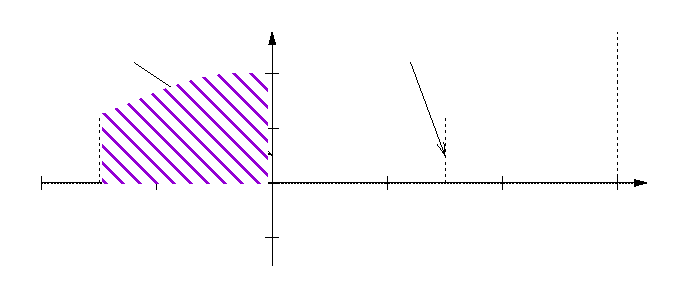
\includegraphics[width={316.80bp},height={129.50bp}]{figura_01_04}}%
    \gplfronttext
  \end{picture}%
\endgroup

    \caption{Demostración gráfica}\label{figura_04}
\end{figure}

\subsection*{Propiedad 4}
Si $b-a=T$:
\begin{equation}
    \int_{0}^{T}f(t)\,dt=\int_{a}^{b}f(t)\,dt
\label{propiedad4}
\end{equation}

\underline{Prueba}:

\begin{equation*}
\begin{split}
    \int_{a}^{b}f(t)\,dt
        &=\int_{a}^{a+T}f(t)\,dt\\
        &=\int_{a}^{T}f(t)\,dt+\int_{T}^{a+T}f(t)\,dt\\
        &=\int_{a}^{T}f(t)\,dt+\int_{T-T}^{a+T-T}f(t)\,dt\\
        &=\int_{a}^{T}f(t)\,dt+\int_{0}^{a}f(t)\,dt\\
        &=\int_{0}^{T}f(t)\,dt
\end{split}
\end{equation*}

Puede verse gráficamente en la \textbf{Figura~\ref{figura_05}}.
\begin{figure}[H]
    \centering
    % GNUPLOT: LaTeX picture with Postscript
\begingroup
  \makeatletter
  \providecommand\color[2][]{%
    \GenericError{(gnuplot) \space\space\space\@spaces}{%
      Package color not loaded in conjunction with
      terminal option `colourtext'%
    }{See the gnuplot documentation for explanation.%
    }{Either use 'blacktext' in gnuplot or load the package
      color.sty in LaTeX.}%
    \renewcommand\color[2][]{}%
  }%
  \providecommand\includegraphics[2][]{%
    \GenericError{(gnuplot) \space\space\space\@spaces}{%
      Package graphicx or graphics not loaded%
    }{See the gnuplot documentation for explanation.%
    }{The gnuplot epslatex terminal needs graphicx.sty or graphics.sty.}%
    \renewcommand\includegraphics[2][]{}%
  }%
  \providecommand\rotatebox[2]{#2}%
  \@ifundefined{ifGPcolor}{%
    \newif\ifGPcolor
    \GPcolorfalse
  }{}%
  \@ifundefined{ifGPblacktext}{%
    \newif\ifGPblacktext
    \GPblacktexttrue
  }{}%
  % define a \g@addto@macro without @ in the name:
  \let\gplgaddtomacro\g@addto@macro
  % define empty templates for all commands taking text:
  \gdef\gplbacktext{}%
  \gdef\gplfronttext{}%
  \makeatother
  \ifGPblacktext
    % no textcolor at all
    \def\colorrgb#1{}%
    \def\colorgray#1{}%
  \else
    % gray or color?
    \ifGPcolor
      \def\colorrgb#1{\color[rgb]{#1}}%
      \def\colorgray#1{\color[gray]{#1}}%
      \expandafter\def\csname LTw\endcsname{\color{white}}%
      \expandafter\def\csname LTb\endcsname{\color{black}}%
      \expandafter\def\csname LTa\endcsname{\color{black}}%
      \expandafter\def\csname LT0\endcsname{\color[rgb]{1,0,0}}%
      \expandafter\def\csname LT1\endcsname{\color[rgb]{0,1,0}}%
      \expandafter\def\csname LT2\endcsname{\color[rgb]{0,0,1}}%
      \expandafter\def\csname LT3\endcsname{\color[rgb]{1,0,1}}%
      \expandafter\def\csname LT4\endcsname{\color[rgb]{0,1,1}}%
      \expandafter\def\csname LT5\endcsname{\color[rgb]{1,1,0}}%
      \expandafter\def\csname LT6\endcsname{\color[rgb]{0,0,0}}%
      \expandafter\def\csname LT7\endcsname{\color[rgb]{1,0.3,0}}%
      \expandafter\def\csname LT8\endcsname{\color[rgb]{0.5,0.5,0.5}}%
    \else
      % gray
      \def\colorrgb#1{\color{black}}%
      \def\colorgray#1{\color[gray]{#1}}%
      \expandafter\def\csname LTw\endcsname{\color{white}}%
      \expandafter\def\csname LTb\endcsname{\color{black}}%
      \expandafter\def\csname LTa\endcsname{\color{black}}%
      \expandafter\def\csname LT0\endcsname{\color{black}}%
      \expandafter\def\csname LT1\endcsname{\color{black}}%
      \expandafter\def\csname LT2\endcsname{\color{black}}%
      \expandafter\def\csname LT3\endcsname{\color{black}}%
      \expandafter\def\csname LT4\endcsname{\color{black}}%
      \expandafter\def\csname LT5\endcsname{\color{black}}%
      \expandafter\def\csname LT6\endcsname{\color{black}}%
      \expandafter\def\csname LT7\endcsname{\color{black}}%
      \expandafter\def\csname LT8\endcsname{\color{black}}%
    \fi
  \fi
    \setlength{\unitlength}{0.0500bp}%
    \ifx\gptboxheight\undefined%
      \newlength{\gptboxheight}%
      \newlength{\gptboxwidth}%
      \newsavebox{\gptboxtext}%
    \fi%
    \setlength{\fboxrule}{0.5pt}%
    \setlength{\fboxsep}{1pt}%
    \definecolor{tbcol}{rgb}{1,1,1}%
\begin{picture}(6336.00,2590.00)%
    \gplgaddtomacro\gplbacktext{%
      \csname LTb\endcsname%%
      \put(1233,416){\makebox(0,0)[r]{\strut{}}}%
      \put(1233,863){\makebox(0,0)[r]{\strut{}}}%
      \put(1233,1311){\makebox(0,0)[r]{\strut{}}}%
      \put(1233,1758){\makebox(0,0)[r]{\strut{}}}%
      \put(1233,2205){\makebox(0,0)[r]{\strut{}}}%
      \put(603,640){\makebox(0,0){\strut{}}}%
      \put(1329,640){\makebox(0,0){\strut{}}}%
      \put(2055,640){\makebox(0,0){\strut{}}}%
      \put(2781,640){\makebox(0,0){\strut{}}}%
      \put(3506,640){\makebox(0,0){\strut{}}}%
      \put(4232,640){\makebox(0,0){\strut{}}}%
      \put(4958,640){\makebox(0,0){\strut{}}}%
      \put(5684,640){\makebox(0,0){\strut{}}}%
      \csname LTb\endcsname%%
      \put(6228,863){\makebox(0,0)[l]{\strut{}$t$}}%
      \put(1502,2429){\makebox(0,0)[l]{\strut{}$f(t)$}}%
      \put(2756,662){\makebox(0,0)[l]{\strut{}$a$}}%
      \put(3435,662){\makebox(0,0)[l]{\strut{}$T$}}%
      \put(4887,662){\makebox(0,0)[l]{\strut{}$b$}}%
      \put(1766,2026){\makebox(0,0)[l]{\strut{}$\int_{0}^{T} f(t) dt$}}%
      \put(3943,2295){\makebox(0,0)[l]{\strut{}$\int_{a}^{b} f(t) dt$}}%
      \put(3770,259){\makebox(0,0)[l]{\strut{}$T$}}%
    }%
    \gplgaddtomacro\gplfronttext{%
    }%
    \gplgaddtomacro\gplbacktext{%
      \csname LTb\endcsname%%
      \put(1233,416){\makebox(0,0)[r]{\strut{}}}%
      \put(1233,863){\makebox(0,0)[r]{\strut{}}}%
      \put(1233,1311){\makebox(0,0)[r]{\strut{}}}%
      \put(1233,1758){\makebox(0,0)[r]{\strut{}}}%
      \put(1233,2205){\makebox(0,0)[r]{\strut{}}}%
      \put(603,640){\makebox(0,0){\strut{}}}%
      \put(1329,640){\makebox(0,0){\strut{}}}%
      \put(2055,640){\makebox(0,0){\strut{}}}%
      \put(2781,640){\makebox(0,0){\strut{}}}%
      \put(3506,640){\makebox(0,0){\strut{}}}%
      \put(4232,640){\makebox(0,0){\strut{}}}%
      \put(4958,640){\makebox(0,0){\strut{}}}%
      \put(5684,640){\makebox(0,0){\strut{}}}%
      \csname LTb\endcsname%%
      \put(6228,863){\makebox(0,0)[l]{\strut{}$t$}}%
      \put(1502,2429){\makebox(0,0)[l]{\strut{}$f(t)$}}%
      \put(2756,662){\makebox(0,0)[l]{\strut{}$a$}}%
      \put(3435,662){\makebox(0,0)[l]{\strut{}$T$}}%
      \put(4887,662){\makebox(0,0)[l]{\strut{}$b$}}%
      \put(1766,2026){\makebox(0,0)[l]{\strut{}$\int_{0}^{T} f(t) dt$}}%
      \put(3943,2295){\makebox(0,0)[l]{\strut{}$\int_{a}^{b} f(t) dt$}}%
      \put(3770,259){\makebox(0,0)[l]{\strut{}$T$}}%
    }%
    \gplgaddtomacro\gplfronttext{%
    }%
    \gplgaddtomacro\gplbacktext{%
      \csname LTb\endcsname%%
      \put(1233,416){\makebox(0,0)[r]{\strut{}}}%
      \put(1233,863){\makebox(0,0)[r]{\strut{}}}%
      \put(1233,1311){\makebox(0,0)[r]{\strut{}}}%
      \put(1233,1758){\makebox(0,0)[r]{\strut{}}}%
      \put(1233,2205){\makebox(0,0)[r]{\strut{}}}%
      \put(603,640){\makebox(0,0){\strut{}}}%
      \put(1329,640){\makebox(0,0){\strut{}}}%
      \put(2055,640){\makebox(0,0){\strut{}}}%
      \put(2781,640){\makebox(0,0){\strut{}}}%
      \put(3506,640){\makebox(0,0){\strut{}}}%
      \put(4232,640){\makebox(0,0){\strut{}}}%
      \put(4958,640){\makebox(0,0){\strut{}}}%
      \put(5684,640){\makebox(0,0){\strut{}}}%
      \csname LTb\endcsname%%
      \put(6228,863){\makebox(0,0)[l]{\strut{}$t$}}%
      \put(1502,2429){\makebox(0,0)[l]{\strut{}$f(t)$}}%
      \put(2756,662){\makebox(0,0)[l]{\strut{}$a$}}%
      \put(3435,662){\makebox(0,0)[l]{\strut{}$T$}}%
      \put(4887,662){\makebox(0,0)[l]{\strut{}$b$}}%
      \put(1766,2026){\makebox(0,0)[l]{\strut{}$\int_{0}^{T} f(t) dt$}}%
      \put(3943,2295){\makebox(0,0)[l]{\strut{}$\int_{a}^{b} f(t) dt$}}%
      \put(3770,259){\makebox(0,0)[l]{\strut{}$T$}}%
    }%
    \gplgaddtomacro\gplfronttext{%
    }%
    \gplgaddtomacro\gplbacktext{%
      \csname LTb\endcsname%%
      \put(1233,416){\makebox(0,0)[r]{\strut{}}}%
      \put(1233,863){\makebox(0,0)[r]{\strut{}}}%
      \put(1233,1311){\makebox(0,0)[r]{\strut{}}}%
      \put(1233,1758){\makebox(0,0)[r]{\strut{}}}%
      \put(1233,2205){\makebox(0,0)[r]{\strut{}}}%
      \put(603,640){\makebox(0,0){\strut{}}}%
      \put(1329,640){\makebox(0,0){\strut{}}}%
      \put(2055,640){\makebox(0,0){\strut{}}}%
      \put(2781,640){\makebox(0,0){\strut{}}}%
      \put(3506,640){\makebox(0,0){\strut{}}}%
      \put(4232,640){\makebox(0,0){\strut{}}}%
      \put(4958,640){\makebox(0,0){\strut{}}}%
      \put(5684,640){\makebox(0,0){\strut{}}}%
      \csname LTb\endcsname%%
      \put(6228,863){\makebox(0,0)[l]{\strut{}$t$}}%
      \put(1502,2429){\makebox(0,0)[l]{\strut{}$f(t)$}}%
      \put(2756,662){\makebox(0,0)[l]{\strut{}$a$}}%
      \put(3435,662){\makebox(0,0)[l]{\strut{}$T$}}%
      \put(4887,662){\makebox(0,0)[l]{\strut{}$b$}}%
      \put(1766,2026){\makebox(0,0)[l]{\strut{}$\int_{0}^{T} f(t) dt$}}%
      \put(3943,2295){\makebox(0,0)[l]{\strut{}$\int_{a}^{b} f(t) dt$}}%
      \put(3770,259){\makebox(0,0)[l]{\strut{}$T$}}%
    }%
    \gplgaddtomacro\gplfronttext{%
    }%
    \gplgaddtomacro\gplbacktext{%
      \csname LTb\endcsname%%
      \put(1233,416){\makebox(0,0)[r]{\strut{}}}%
      \put(1233,863){\makebox(0,0)[r]{\strut{}}}%
      \put(1233,1311){\makebox(0,0)[r]{\strut{}}}%
      \put(1233,1758){\makebox(0,0)[r]{\strut{}}}%
      \put(1233,2205){\makebox(0,0)[r]{\strut{}}}%
      \put(603,640){\makebox(0,0){\strut{}}}%
      \put(1329,640){\makebox(0,0){\strut{}}}%
      \put(2055,640){\makebox(0,0){\strut{}}}%
      \put(2781,640){\makebox(0,0){\strut{}}}%
      \put(3506,640){\makebox(0,0){\strut{}}}%
      \put(4232,640){\makebox(0,0){\strut{}}}%
      \put(4958,640){\makebox(0,0){\strut{}}}%
      \put(5684,640){\makebox(0,0){\strut{}}}%
      \csname LTb\endcsname%%
      \put(6228,863){\makebox(0,0)[l]{\strut{}$t$}}%
      \put(1502,2429){\makebox(0,0)[l]{\strut{}$f(t)$}}%
      \put(2756,662){\makebox(0,0)[l]{\strut{}$a$}}%
      \put(3435,662){\makebox(0,0)[l]{\strut{}$T$}}%
      \put(4887,662){\makebox(0,0)[l]{\strut{}$b$}}%
      \put(1766,2026){\makebox(0,0)[l]{\strut{}$\int_{0}^{T} f(t) dt$}}%
      \put(3943,2295){\makebox(0,0)[l]{\strut{}$\int_{a}^{b} f(t) dt$}}%
      \put(3770,259){\makebox(0,0)[l]{\strut{}$T$}}%
    }%
    \gplgaddtomacro\gplfronttext{%
    }%
    \gplgaddtomacro\gplbacktext{%
      \csname LTb\endcsname%%
      \put(1233,416){\makebox(0,0)[r]{\strut{}}}%
      \put(1233,863){\makebox(0,0)[r]{\strut{}}}%
      \put(1233,1311){\makebox(0,0)[r]{\strut{}}}%
      \put(1233,1758){\makebox(0,0)[r]{\strut{}}}%
      \put(1233,2205){\makebox(0,0)[r]{\strut{}}}%
      \put(603,640){\makebox(0,0){\strut{}}}%
      \put(1329,640){\makebox(0,0){\strut{}}}%
      \put(2055,640){\makebox(0,0){\strut{}}}%
      \put(2781,640){\makebox(0,0){\strut{}}}%
      \put(3506,640){\makebox(0,0){\strut{}}}%
      \put(4232,640){\makebox(0,0){\strut{}}}%
      \put(4958,640){\makebox(0,0){\strut{}}}%
      \put(5684,640){\makebox(0,0){\strut{}}}%
      \csname LTb\endcsname%%
      \put(6228,863){\makebox(0,0)[l]{\strut{}$t$}}%
      \put(1502,2429){\makebox(0,0)[l]{\strut{}$f(t)$}}%
      \put(2756,662){\makebox(0,0)[l]{\strut{}$a$}}%
      \put(3435,662){\makebox(0,0)[l]{\strut{}$T$}}%
      \put(4887,662){\makebox(0,0)[l]{\strut{}$b$}}%
      \put(1766,2026){\makebox(0,0)[l]{\strut{}$\int_{0}^{T} f(t) dt$}}%
      \put(3943,2295){\makebox(0,0)[l]{\strut{}$\int_{a}^{b} f(t) dt$}}%
      \put(3770,259){\makebox(0,0)[l]{\strut{}$T$}}%
    }%
    \gplgaddtomacro\gplfronttext{%
    }%
    \gplgaddtomacro\gplbacktext{%
      \csname LTb\endcsname%%
      \put(1233,416){\makebox(0,0)[r]{\strut{}}}%
      \put(1233,863){\makebox(0,0)[r]{\strut{}}}%
      \put(1233,1311){\makebox(0,0)[r]{\strut{}}}%
      \put(1233,1758){\makebox(0,0)[r]{\strut{}}}%
      \put(1233,2205){\makebox(0,0)[r]{\strut{}}}%
      \put(603,640){\makebox(0,0){\strut{}}}%
      \put(1329,640){\makebox(0,0){\strut{}}}%
      \put(2055,640){\makebox(0,0){\strut{}}}%
      \put(2781,640){\makebox(0,0){\strut{}}}%
      \put(3506,640){\makebox(0,0){\strut{}}}%
      \put(4232,640){\makebox(0,0){\strut{}}}%
      \put(4958,640){\makebox(0,0){\strut{}}}%
      \put(5684,640){\makebox(0,0){\strut{}}}%
      \csname LTb\endcsname%%
      \put(6228,863){\makebox(0,0)[l]{\strut{}$t$}}%
      \put(1502,2429){\makebox(0,0)[l]{\strut{}$f(t)$}}%
      \put(2756,662){\makebox(0,0)[l]{\strut{}$a$}}%
      \put(3435,662){\makebox(0,0)[l]{\strut{}$T$}}%
      \put(4887,662){\makebox(0,0)[l]{\strut{}$b$}}%
      \put(1766,2026){\makebox(0,0)[l]{\strut{}$\int_{0}^{T} f(t) dt$}}%
      \put(3943,2295){\makebox(0,0)[l]{\strut{}$\int_{a}^{b} f(t) dt$}}%
      \put(3770,259){\makebox(0,0)[l]{\strut{}$T$}}%
    }%
    \gplgaddtomacro\gplfronttext{%
    }%
    \gplbacktext
    \put(0,0){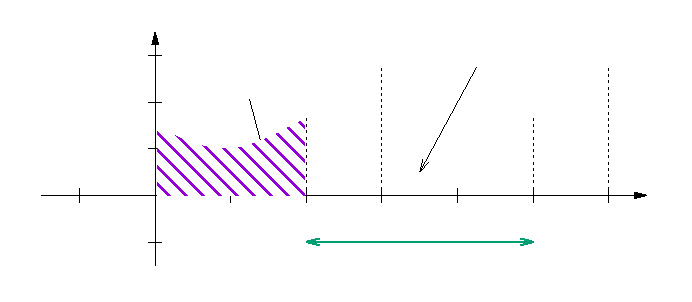
\includegraphics[width={316.80bp},height={129.50bp}]{figura_01_05}}%
    \gplfronttext
  \end{picture}%
\endgroup

    \caption{Demostración gráfica}\label{figura_05}
\end{figure}

\subsection{Funciones seno y coseno}
\begin{equation*}
    f(t)=A\,\sen(\omega_0\,t)
\end{equation*}
\begin{equation*}
    f(t)=A\,\cos(\omega_0\,t)
\end{equation*}

Donde:\\
\indent\indent$A$: Amplitud.\\
\indent\indent$\omega_0$: Frecuencia angular.\\
\indent\indent$T=2\pi/\omega_0$: Periodo.\\

\textbf{Ejemplo}: Hallar el periodo de la siguiente función:
\begin{equation*}
    f(t)=\sen(4t)+\sen(3t/2)+\sen(10t)
\end{equation*}

El periodo buscado debe contener un numero entero de veces a los 3 periodos
hallados:
\begin{equation*}
    T=\begin{cases}
        a\,T_1;&\,a\in\mathbb{N}\\
        b\,T_2;&\,b\in\mathbb{N}\\
        c\,T_3;&\,c\in\mathbb{N}\\
    \end{cases}
\end{equation*}
\begin{equation*}
    a\,T_1=b\,T_2=c\,T_3
\end{equation*}
\begin{equation*}
    a\,\frac{2\pi}{4}=b\,\frac{2\pi}{3/2}=c\,\frac{2\pi}{10}
\end{equation*}
\begin{equation*}
    a\,\frac{\pi}{2}=b\,\frac{4\pi}{3}=c\,\frac{\pi}{5};x30
\end{equation*}
\begin{equation*}
    15a=40b=6c
\end{equation*}
\begin{equation*}
    M.C.M.(15,40,6)=120
\end{equation*}
\begin{equation*}
\left.\begin{aligned}
    120=15a\rightarrow\,a=8\\
    120=40b\rightarrow\,b=3\\
    120=6c\rightarrow\,c=20\\
\end{aligned}\right\}=T=8\left(\frac{\pi}{2}\right)=4\pi
\end{equation*}

Puede verse gráficamente en la \textbf{Figura~\ref{figura_06}}.
\begin{figure}[H]
    \centering
    % GNUPLOT: LaTeX picture with Postscript
\begingroup
  \makeatletter
  \providecommand\color[2][]{%
    \GenericError{(gnuplot) \space\space\space\@spaces}{%
      Package color not loaded in conjunction with
      terminal option `colourtext'%
    }{See the gnuplot documentation for explanation.%
    }{Either use 'blacktext' in gnuplot or load the package
      color.sty in LaTeX.}%
    \renewcommand\color[2][]{}%
  }%
  \providecommand\includegraphics[2][]{%
    \GenericError{(gnuplot) \space\space\space\@spaces}{%
      Package graphicx or graphics not loaded%
    }{See the gnuplot documentation for explanation.%
    }{The gnuplot epslatex terminal needs graphicx.sty or graphics.sty.}%
    \renewcommand\includegraphics[2][]{}%
  }%
  \providecommand\rotatebox[2]{#2}%
  \@ifundefined{ifGPcolor}{%
    \newif\ifGPcolor
    \GPcolorfalse
  }{}%
  \@ifundefined{ifGPblacktext}{%
    \newif\ifGPblacktext
    \GPblacktexttrue
  }{}%
  % define a \g@addto@macro without @ in the name:
  \let\gplgaddtomacro\g@addto@macro
  % define empty templates for all commands taking text:
  \gdef\gplbacktext{}%
  \gdef\gplfronttext{}%
  \makeatother
  \ifGPblacktext
    % no textcolor at all
    \def\colorrgb#1{}%
    \def\colorgray#1{}%
  \else
    % gray or color?
    \ifGPcolor
      \def\colorrgb#1{\color[rgb]{#1}}%
      \def\colorgray#1{\color[gray]{#1}}%
      \expandafter\def\csname LTw\endcsname{\color{white}}%
      \expandafter\def\csname LTb\endcsname{\color{black}}%
      \expandafter\def\csname LTa\endcsname{\color{black}}%
      \expandafter\def\csname LT0\endcsname{\color[rgb]{1,0,0}}%
      \expandafter\def\csname LT1\endcsname{\color[rgb]{0,1,0}}%
      \expandafter\def\csname LT2\endcsname{\color[rgb]{0,0,1}}%
      \expandafter\def\csname LT3\endcsname{\color[rgb]{1,0,1}}%
      \expandafter\def\csname LT4\endcsname{\color[rgb]{0,1,1}}%
      \expandafter\def\csname LT5\endcsname{\color[rgb]{1,1,0}}%
      \expandafter\def\csname LT6\endcsname{\color[rgb]{0,0,0}}%
      \expandafter\def\csname LT7\endcsname{\color[rgb]{1,0.3,0}}%
      \expandafter\def\csname LT8\endcsname{\color[rgb]{0.5,0.5,0.5}}%
    \else
      % gray
      \def\colorrgb#1{\color{black}}%
      \def\colorgray#1{\color[gray]{#1}}%
      \expandafter\def\csname LTw\endcsname{\color{white}}%
      \expandafter\def\csname LTb\endcsname{\color{black}}%
      \expandafter\def\csname LTa\endcsname{\color{black}}%
      \expandafter\def\csname LT0\endcsname{\color{black}}%
      \expandafter\def\csname LT1\endcsname{\color{black}}%
      \expandafter\def\csname LT2\endcsname{\color{black}}%
      \expandafter\def\csname LT3\endcsname{\color{black}}%
      \expandafter\def\csname LT4\endcsname{\color{black}}%
      \expandafter\def\csname LT5\endcsname{\color{black}}%
      \expandafter\def\csname LT6\endcsname{\color{black}}%
      \expandafter\def\csname LT7\endcsname{\color{black}}%
      \expandafter\def\csname LT8\endcsname{\color{black}}%
    \fi
  \fi
    \setlength{\unitlength}{0.0500bp}%
    \ifx\gptboxheight\undefined%
      \newlength{\gptboxheight}%
      \newlength{\gptboxwidth}%
      \newsavebox{\gptboxtext}%
    \fi%
    \setlength{\fboxrule}{0.5pt}%
    \setlength{\fboxsep}{1pt}%
    \definecolor{tbcol}{rgb}{1,1,1}%
\begin{picture}(6336.00,1872.00)%
    \gplgaddtomacro\gplbacktext{%
      \csname LTb\endcsname%%
      \put(144,276){\makebox(0,0)[r]{\strut{}}}%
      \put(144,445){\makebox(0,0)[r]{\strut{}}}%
      \put(144,614){\makebox(0,0)[r]{\strut{}}}%
      \put(144,783){\makebox(0,0)[r]{\strut{}}}%
      \put(144,952){\makebox(0,0)[r]{\strut{}}}%
      \put(144,1120){\makebox(0,0)[r]{\strut{}}}%
      \put(144,1289){\makebox(0,0)[r]{\strut{}}}%
      \put(144,1458){\makebox(0,0)[r]{\strut{}}}%
      \put(144,1627){\makebox(0,0)[r]{\strut{}}}%
      \put(240,560){\makebox(0,0){\strut{}}}%
      \put(1606,560){\makebox(0,0){\strut{}}}%
      \put(2973,560){\makebox(0,0){\strut{}}}%
      \put(4339,560){\makebox(0,0){\strut{}}}%
      \put(5705,560){\makebox(0,0){\strut{}}}%
      \csname LTb\endcsname%%
      \put(6184,783){\makebox(0,0)[l]{\strut{}$t$}}%
      \put(392,1711){\makebox(0,0)[l]{\strut{}$f(t)$}}%
      \put(1541,656){\makebox(0,0)[l]{\strut{}$ \pi$}}%
      \put(2907,656){\makebox(0,0)[l]{\strut{}$2\pi$}}%
      \put(4274,656){\makebox(0,0)[l]{\strut{}$3\pi$}}%
      \put(5640,656){\makebox(0,0)[l]{\strut{}$4\pi$}}%
      \put(1606,1593){\makebox(0,0)[l]{\strut{}$f(t)=\sen(4t)+\sen(\frac{3}{2}t)+\sen(10t)\,dt$}}%
    }%
    \gplgaddtomacro\gplfronttext{%
    }%
    \gplbacktext
    \put(0,0){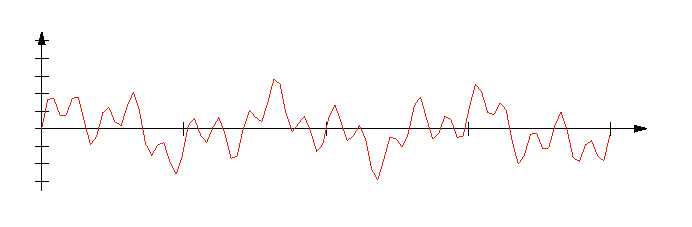
\includegraphics[width={316.80bp},height={93.60bp}]{figura_01_06}}%
    \gplfronttext
  \end{picture}%
\endgroup

    \caption{Periodo de la función}\label{figura_06}
\end{figure}

\subsection{Propiedades ortogonales del seno y el coseno}
\subsection*{Propiedad 1}
\begin{equation}
    \int_{0}^{T}\sen(n\omega_0\,t)\,dt=0\quad\,n\in\mathbb{Z}
\end{equation}

\underline{Prueba}:

\begin{equation*}
\begin{split}
    \int_{0}^{T}\sen(n\omega_0\,t)\,dt
        &=-\frac{\cos(n\omega_0\,t)}{n\omega_0}\Biggr|_{0}^{T}\\
        &=-\frac{\cos(n\omega_0\,T)}{n\omega_0}+\frac{\cos(0)}{n\omega_0}\\
        &=-\frac{\cos(n\,2\pi)}{n\omega_0}+\frac{\cos(0)}{n\omega_0}\\
        &=-\frac{1}{n\omega_0}+\frac{1}{n\omega_0}\\
        &=0\\
\end{split}
\end{equation*}
\begin{equation}
    \int_{0}^{T}\cos(n\omega_0\,t)\,dt=0\quad\,n\in\mathbb{Z}
\end{equation}

\underline{Prueba}:

\begin{equation*}
\begin{split}
    \int_{0}^{T}\cos(n\omega_0\,t)\,dt
        &=\frac{\sen(n\omega_0\,t)}{n\omega_0}\Biggr|_{0}^{T}\\
        &=\frac{\sen(n\omega_0\,T)}{n\omega_0}-\frac{\sen(0)}{n\omega_0}\\
        &=\frac{\sen(n\,2\pi)}{n\omega_0}-\frac{\sen(0)}{n\omega_0}\\
        &=\frac{0}{n\omega_0}-\frac{0}{n\omega_0}\\
        &=0\\
\end{split}
\end{equation*}

\subsection*{Propiedad 2}
\begin{equation}
    \int_{0}^{T}\sen(m\omega_0\,t)\sen(n\omega_0\,t)\,dt=0
    \quad\,m,n\,\in\mathbb{Z}\quad\,m\neq\,n
\end{equation}

\underline{Prueba}:

\begin{equation*}
\begin{split}
    \int_{0}^{T}\sen(m\omega_0\,t)\sen(n\omega_0\,t)\,dt
        &=\int_{0}^{T}\frac{1}{2}(\cos((m-n)\omega_0\,t)-
          \cos((m+n)\omega_0\,t))dt\\
        &=\frac{1}{2}\left(\int_{0}^{T}\cos((m-n)\omega_0\,t)dt-
          \int_{0}^{T}\cos((m+n)\omega_0\,t)dt\right)\\
        &=\frac{1}{2}(0-0)\\
        &=0\\
\end{split}
\end{equation*}
\begin{equation}
    \int_{0}^{T}\cos(m\omega_0\,t)\cos(n\omega_0\,t)\,dt=0
    \quad\,m,n\,\in\mathbb{Z}\quad\,m\neq\,n
\end{equation}

\underline{Prueba}:

\begin{equation*}
\begin{split}
    \int_{0}^{T}\cos(m\omega_0\,t)\cos(n\omega_0\,t)\,dt
        &=\int_{0}^{T}\frac{1}{2}(\cos((m-n)\omega_0\,t)+
          \cos((m+n)\omega_0\,t))dt\\
        &=\frac{1}{2}\left(\int_{0}^{T}\cos((m-n)\omega_0\,t)dt+
          \int_{0}^{T}\cos((m+n)\omega_0\,t)dt\right)\\
        &=\frac{1}{2}(0+0)\\
        &=0\\
\end{split}
\end{equation*}
\begin{equation}
    \int_{0}^{T}\sen(m\omega_0\,t)\cos(n\omega_0\,t)\,dt
    =0\quad\,m,n\,\in\mathbb{Z}
\end{equation}

\underline{Prueba}:

\begin{equation*}
\begin{split}
    \int_{0}^{T}\sen(m\omega_0\,t)\cos(n\omega_0\,t)\,dt
        &=\int_{0}^{T}\frac{1}{2}(\sen((m-n)\omega_0\,t)+
          \sen((m+n)\omega_0\,t))dt\\
        &=\frac{1}{2}\left(\int_{0}^{T}\sen((m-n)\omega_0\,t)dt+
          \int_{0}^{T}\cos((m+n)\omega_0\,t)dt\right)\\
        &=\frac{1}{2}(0+0)\\
        &=0\\
\end{split}
\end{equation*}

\subsection*{Propiedad 3}
\begin{equation}
    \int_{0}^{T}\sen^2(n\omega_0\,t)\,dt=\frac{T}{2}\quad\,n\,\in\mathbb{Z}
\end{equation}

\underline{Prueba}:

\begin{equation*}
\begin{split}
    \int_{0}^{T}\sen^2(n\omega_0\,t)\,dt
        &=\int_{0}^{T}\sen(n\omega_0\,t)\sen(n\omega_0\,t)dt\\
        &=\frac{1}{2}\left(\int_{0}^{T}\cos((n-n)\omega_0\,t)dt-
          \int_{0}^{T}\cos((n+n)\omega_0\,t)dt\right)\\
        &=\frac{1}{2}\left(\int_{0}^{T}\cos(0)dt-
          \int_{0}^{T}\cos((2n)\omega_0\,t)dt\right)\\
        &=\frac{1}{2}\left(\int_{0}^{T}dt-
          \int_{0}^{T}\cos(2n\omega_0\,t)dt\right)\\
        &=\frac{1}{2}(t\Biggr|_0^T-0)\\
        &=\frac{T}{2}\\
\end{split}
\end{equation*}
\begin{equation}
    \int_{0}^{T}\cos^2(n\omega_0\,t)\,dt=\frac{T}{2}\quad\,n\,\in\mathbb{Z}
\end{equation}

\underline{Prueba}:

\begin{equation*}
\begin{split}
    \int_{0}^{T}\cos^2(n\omega_0\,t)\,dt
        &=\int_{0}^{T}\cos(n\omega_0\,t)\cos(n\omega_0\,t)dt\\
        &=\frac{1}{2}\left(\int_{0}^{T}\cos((n-n)\omega_0\,t)dt+
          \int_{0}^{T}\cos((n+n)\omega_0\,t)dt\right)\\
        &=\frac{1}{2}\left(\int_{0}^{T}\cos(0)dt+
          \int_{0}^{T}\cos((2n)\omega_0\,t)dt\right)\\
        &=\frac{1}{2}\left(\int_{0}^{T}dt+
          \int_{0}^{T}\cos(2n\omega_0\,t)dt\right)\\
        &=\frac{1}{2}(t\Biggr|_0^T+0)\\
        &=\frac{T}{2}\\
\end{split}
\end{equation*}

\section{Series de \emph{Fourier}}
Una función periódica que cumple ciertas condiciones puede desarrollarse
mediante la serie:
\begin{equation}
    f(t)=\frac{a_0}{2}+
    \sum_{n=1}^{\infty}[a_n\cos(n\omega_0\,t)+b_n\sen(n\omega_0\,t)]
\end{equation}

Donde:\\
\indent\indent$\omega_0=2\pi/T$: Frecuencia angular de $f(t)$.\\
\indent\indent$T$: Periodo de $f(t)$.\\
\indent\indent$a_0;a_n;b_n$: Coeficientes de \emph{Fourier}.\\
\indent\indent$a_0/2$: Termino constante.\\
\indent\indent$a_n\cos(n\omega_0\,t);b_n\sen(n\omega_0\,t)$: Armónicos, términos
seno y coseno con frecuencias angulares múltiples de $\omega_0$\\

\indent\indent$a_1\cos(\omega_0\,t)+b_1\sen(\omega_0\,t)$: Primer armónico.\\
\indent\indent$a_2\cos(2\omega_0\,t)+b_2\sen(2\omega_0\,t)$: Segundo armónico.\\
\indent\indent$a_3\cos(3\omega_0\,t)+b_3\sen(2\omega_0\,t)$: Tercer armónico.\\

\subsection{Condiciones de \emph{Dirichlet}}
Para que una función periódica $f(t)=f(t+nT);\,n\in\mathbb{Z}$, se desarrolle
como una serie de \emph{Fourier} debe cumplir:

\begin{itemize}
\item $f(t)$ debe ser continua por tramos en 1 periodo.
    \begin{figure}[H]
        \centering
        % GNUPLOT: LaTeX picture with Postscript
\begingroup
  \makeatletter
  \providecommand\color[2][]{%
    \GenericError{(gnuplot) \space\space\space\@spaces}{%
      Package color not loaded in conjunction with
      terminal option `colourtext'%
    }{See the gnuplot documentation for explanation.%
    }{Either use 'blacktext' in gnuplot or load the package
      color.sty in LaTeX.}%
    \renewcommand\color[2][]{}%
  }%
  \providecommand\includegraphics[2][]{%
    \GenericError{(gnuplot) \space\space\space\@spaces}{%
      Package graphicx or graphics not loaded%
    }{See the gnuplot documentation for explanation.%
    }{The gnuplot epslatex terminal needs graphicx.sty or graphics.sty.}%
    \renewcommand\includegraphics[2][]{}%
  }%
  \providecommand\rotatebox[2]{#2}%
  \@ifundefined{ifGPcolor}{%
    \newif\ifGPcolor
    \GPcolorfalse
  }{}%
  \@ifundefined{ifGPblacktext}{%
    \newif\ifGPblacktext
    \GPblacktexttrue
  }{}%
  % define a \g@addto@macro without @ in the name:
  \let\gplgaddtomacro\g@addto@macro
  % define empty templates for all commands taking text:
  \gdef\gplbacktext{}%
  \gdef\gplfronttext{}%
  \makeatother
  \ifGPblacktext
    % no textcolor at all
    \def\colorrgb#1{}%
    \def\colorgray#1{}%
  \else
    % gray or color?
    \ifGPcolor
      \def\colorrgb#1{\color[rgb]{#1}}%
      \def\colorgray#1{\color[gray]{#1}}%
      \expandafter\def\csname LTw\endcsname{\color{white}}%
      \expandafter\def\csname LTb\endcsname{\color{black}}%
      \expandafter\def\csname LTa\endcsname{\color{black}}%
      \expandafter\def\csname LT0\endcsname{\color[rgb]{1,0,0}}%
      \expandafter\def\csname LT1\endcsname{\color[rgb]{0,1,0}}%
      \expandafter\def\csname LT2\endcsname{\color[rgb]{0,0,1}}%
      \expandafter\def\csname LT3\endcsname{\color[rgb]{1,0,1}}%
      \expandafter\def\csname LT4\endcsname{\color[rgb]{0,1,1}}%
      \expandafter\def\csname LT5\endcsname{\color[rgb]{1,1,0}}%
      \expandafter\def\csname LT6\endcsname{\color[rgb]{0,0,0}}%
      \expandafter\def\csname LT7\endcsname{\color[rgb]{1,0.3,0}}%
      \expandafter\def\csname LT8\endcsname{\color[rgb]{0.5,0.5,0.5}}%
    \else
      % gray
      \def\colorrgb#1{\color{black}}%
      \def\colorgray#1{\color[gray]{#1}}%
      \expandafter\def\csname LTw\endcsname{\color{white}}%
      \expandafter\def\csname LTb\endcsname{\color{black}}%
      \expandafter\def\csname LTa\endcsname{\color{black}}%
      \expandafter\def\csname LT0\endcsname{\color{black}}%
      \expandafter\def\csname LT1\endcsname{\color{black}}%
      \expandafter\def\csname LT2\endcsname{\color{black}}%
      \expandafter\def\csname LT3\endcsname{\color{black}}%
      \expandafter\def\csname LT4\endcsname{\color{black}}%
      \expandafter\def\csname LT5\endcsname{\color{black}}%
      \expandafter\def\csname LT6\endcsname{\color{black}}%
      \expandafter\def\csname LT7\endcsname{\color{black}}%
      \expandafter\def\csname LT8\endcsname{\color{black}}%
    \fi
  \fi
    \setlength{\unitlength}{0.0500bp}%
    \ifx\gptboxheight\undefined%
      \newlength{\gptboxheight}%
      \newlength{\gptboxwidth}%
      \newsavebox{\gptboxtext}%
    \fi%
    \setlength{\fboxrule}{0.5pt}%
    \setlength{\fboxsep}{1pt}%
    \definecolor{tbcol}{rgb}{1,1,1}%
\begin{picture}(6336.00,2590.00)%
    \gplgaddtomacro\gplbacktext{%
      \csname LTb\endcsname%%
      \put(628,352){\makebox(0,0)[r]{\strut{}}}%
      \put(628,671){\makebox(0,0)[r]{\strut{}}}%
      \put(628,991){\makebox(0,0)[r]{\strut{}}}%
      \put(628,1311){\makebox(0,0)[r]{\strut{}}}%
      \put(628,1630){\makebox(0,0)[r]{\strut{}}}%
      \put(628,1950){\makebox(0,0)[r]{\strut{}}}%
      \put(628,2269){\makebox(0,0)[r]{\strut{}}}%
      \put(724,1088){\makebox(0,0){\strut{}}}%
      \put(1692,1088){\makebox(0,0){\strut{}}}%
      \put(2660,1088){\makebox(0,0){\strut{}}}%
      \put(3627,1088){\makebox(0,0){\strut{}}}%
      \put(4595,1088){\makebox(0,0){\strut{}}}%
      \put(5563,1088){\makebox(0,0){\strut{}}}%
      \csname LTb\endcsname%%
      \put(6289,1311){\makebox(0,0)[l]{\strut{}$t$}}%
      \put(579,2589){\makebox(0,0)[l]{\strut{}$f(t)$}}%
      \put(2611,1071){\makebox(0,0)[l]{\strut{}$t_1$}}%
      \put(3579,1071){\makebox(0,0)[l]{\strut{}$t_2$}}%
      \put(5515,1071){\makebox(0,0)[l]{\strut{}$T$}}%
      \put(3627,2333){\makebox(0,0)[l]{\strut{}discontinuidad}}%
      \put(4111,2014){\makebox(0,0)[l]{\strut{}extremo relativo}}%
    }%
    \gplgaddtomacro\gplfronttext{%
    }%
    \gplgaddtomacro\gplbacktext{%
      \csname LTb\endcsname%%
      \put(628,352){\makebox(0,0)[r]{\strut{}}}%
      \put(628,671){\makebox(0,0)[r]{\strut{}}}%
      \put(628,991){\makebox(0,0)[r]{\strut{}}}%
      \put(628,1311){\makebox(0,0)[r]{\strut{}}}%
      \put(628,1630){\makebox(0,0)[r]{\strut{}}}%
      \put(628,1950){\makebox(0,0)[r]{\strut{}}}%
      \put(628,2269){\makebox(0,0)[r]{\strut{}}}%
      \put(724,1088){\makebox(0,0){\strut{}}}%
      \put(1692,1088){\makebox(0,0){\strut{}}}%
      \put(2660,1088){\makebox(0,0){\strut{}}}%
      \put(3627,1088){\makebox(0,0){\strut{}}}%
      \put(4595,1088){\makebox(0,0){\strut{}}}%
      \put(5563,1088){\makebox(0,0){\strut{}}}%
      \csname LTb\endcsname%%
      \put(6289,1311){\makebox(0,0)[l]{\strut{}$t$}}%
      \put(579,2589){\makebox(0,0)[l]{\strut{}$f(t)$}}%
      \put(2611,1071){\makebox(0,0)[l]{\strut{}$t_1$}}%
      \put(3579,1071){\makebox(0,0)[l]{\strut{}$t_2$}}%
      \put(5515,1071){\makebox(0,0)[l]{\strut{}$T$}}%
      \put(3627,2333){\makebox(0,0)[l]{\strut{}discontinuidad}}%
      \put(4111,2014){\makebox(0,0)[l]{\strut{}extremo relativo}}%
    }%
    \gplgaddtomacro\gplfronttext{%
    }%
    \gplgaddtomacro\gplbacktext{%
      \csname LTb\endcsname%%
      \put(628,352){\makebox(0,0)[r]{\strut{}}}%
      \put(628,671){\makebox(0,0)[r]{\strut{}}}%
      \put(628,991){\makebox(0,0)[r]{\strut{}}}%
      \put(628,1311){\makebox(0,0)[r]{\strut{}}}%
      \put(628,1630){\makebox(0,0)[r]{\strut{}}}%
      \put(628,1950){\makebox(0,0)[r]{\strut{}}}%
      \put(628,2269){\makebox(0,0)[r]{\strut{}}}%
      \put(724,1088){\makebox(0,0){\strut{}}}%
      \put(1692,1088){\makebox(0,0){\strut{}}}%
      \put(2660,1088){\makebox(0,0){\strut{}}}%
      \put(3627,1088){\makebox(0,0){\strut{}}}%
      \put(4595,1088){\makebox(0,0){\strut{}}}%
      \put(5563,1088){\makebox(0,0){\strut{}}}%
      \csname LTb\endcsname%%
      \put(6289,1311){\makebox(0,0)[l]{\strut{}$t$}}%
      \put(579,2589){\makebox(0,0)[l]{\strut{}$f(t)$}}%
      \put(2611,1071){\makebox(0,0)[l]{\strut{}$t_1$}}%
      \put(3579,1071){\makebox(0,0)[l]{\strut{}$t_2$}}%
      \put(5515,1071){\makebox(0,0)[l]{\strut{}$T$}}%
      \put(3627,2333){\makebox(0,0)[l]{\strut{}discontinuidad}}%
      \put(4111,2014){\makebox(0,0)[l]{\strut{}extremo relativo}}%
    }%
    \gplgaddtomacro\gplfronttext{%
    }%
    \gplbacktext
    \put(0,0){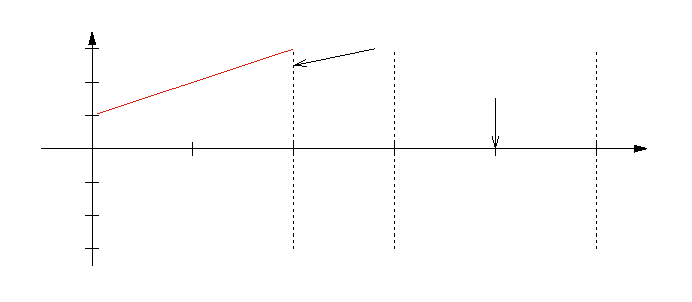
\includegraphics[width={316.80bp},height={129.50bp}]{figura_01_07}}%
    \gplfronttext
  \end{picture}%
\endgroup

    \end{figure}
    \begin{itemize}
    \item Debe existir un numero finito de discontinuidades (en 1 periodo).
    \item Debe existir un numero finito de extremos relativos (en 1 periodo).
    \end{itemize}
\item La integral $\int_0^T|f(t)|\,dt<\infty$ debe ser finita.
\end{itemize}

\textbf{Ejemplo}:
\begin{equation*}
    f(t)=\tan(t);\quad\,0<t<\pi;\quad\,T=\pi
\end{equation*}
\begin{figure}[H]
    \centering
    % GNUPLOT: LaTeX picture with Postscript
\begingroup
  \makeatletter
  \providecommand\color[2][]{%
    \GenericError{(gnuplot) \space\space\space\@spaces}{%
      Package color not loaded in conjunction with
      terminal option `colourtext'%
    }{See the gnuplot documentation for explanation.%
    }{Either use 'blacktext' in gnuplot or load the package
      color.sty in LaTeX.}%
    \renewcommand\color[2][]{}%
  }%
  \providecommand\includegraphics[2][]{%
    \GenericError{(gnuplot) \space\space\space\@spaces}{%
      Package graphicx or graphics not loaded%
    }{See the gnuplot documentation for explanation.%
    }{The gnuplot epslatex terminal needs graphicx.sty or graphics.sty.}%
    \renewcommand\includegraphics[2][]{}%
  }%
  \providecommand\rotatebox[2]{#2}%
  \@ifundefined{ifGPcolor}{%
    \newif\ifGPcolor
    \GPcolorfalse
  }{}%
  \@ifundefined{ifGPblacktext}{%
    \newif\ifGPblacktext
    \GPblacktexttrue
  }{}%
  % define a \g@addto@macro without @ in the name:
  \let\gplgaddtomacro\g@addto@macro
  % define empty templates for all commands taking text:
  \gdef\gplbacktext{}%
  \gdef\gplfronttext{}%
  \makeatother
  \ifGPblacktext
    % no textcolor at all
    \def\colorrgb#1{}%
    \def\colorgray#1{}%
  \else
    % gray or color?
    \ifGPcolor
      \def\colorrgb#1{\color[rgb]{#1}}%
      \def\colorgray#1{\color[gray]{#1}}%
      \expandafter\def\csname LTw\endcsname{\color{white}}%
      \expandafter\def\csname LTb\endcsname{\color{black}}%
      \expandafter\def\csname LTa\endcsname{\color{black}}%
      \expandafter\def\csname LT0\endcsname{\color[rgb]{1,0,0}}%
      \expandafter\def\csname LT1\endcsname{\color[rgb]{0,1,0}}%
      \expandafter\def\csname LT2\endcsname{\color[rgb]{0,0,1}}%
      \expandafter\def\csname LT3\endcsname{\color[rgb]{1,0,1}}%
      \expandafter\def\csname LT4\endcsname{\color[rgb]{0,1,1}}%
      \expandafter\def\csname LT5\endcsname{\color[rgb]{1,1,0}}%
      \expandafter\def\csname LT6\endcsname{\color[rgb]{0,0,0}}%
      \expandafter\def\csname LT7\endcsname{\color[rgb]{1,0.3,0}}%
      \expandafter\def\csname LT8\endcsname{\color[rgb]{0.5,0.5,0.5}}%
    \else
      % gray
      \def\colorrgb#1{\color{black}}%
      \def\colorgray#1{\color[gray]{#1}}%
      \expandafter\def\csname LTw\endcsname{\color{white}}%
      \expandafter\def\csname LTb\endcsname{\color{black}}%
      \expandafter\def\csname LTa\endcsname{\color{black}}%
      \expandafter\def\csname LT0\endcsname{\color{black}}%
      \expandafter\def\csname LT1\endcsname{\color{black}}%
      \expandafter\def\csname LT2\endcsname{\color{black}}%
      \expandafter\def\csname LT3\endcsname{\color{black}}%
      \expandafter\def\csname LT4\endcsname{\color{black}}%
      \expandafter\def\csname LT5\endcsname{\color{black}}%
      \expandafter\def\csname LT6\endcsname{\color{black}}%
      \expandafter\def\csname LT7\endcsname{\color{black}}%
      \expandafter\def\csname LT8\endcsname{\color{black}}%
    \fi
  \fi
    \setlength{\unitlength}{0.0500bp}%
    \ifx\gptboxheight\undefined%
      \newlength{\gptboxheight}%
      \newlength{\gptboxwidth}%
      \newsavebox{\gptboxtext}%
    \fi%
    \setlength{\fboxrule}{0.5pt}%
    \setlength{\fboxsep}{1pt}%
    \definecolor{tbcol}{rgb}{1,1,1}%
\begin{picture}(4320.00,4320.00)%
    \gplgaddtomacro\gplbacktext{%
      \csname LTb\endcsname%%
      \put(2040,192){\makebox(0,0)[r]{\strut{}}}%
      \put(2040,390){\makebox(0,0)[r]{\strut{}}}%
      \put(2040,589){\makebox(0,0)[r]{\strut{}}}%
      \put(2040,787){\makebox(0,0)[r]{\strut{}}}%
      \put(2040,985){\makebox(0,0)[r]{\strut{}}}%
      \put(2040,1184){\makebox(0,0)[r]{\strut{}}}%
      \put(2040,1382){\makebox(0,0)[r]{\strut{}}}%
      \put(2040,1580){\makebox(0,0)[r]{\strut{}}}%
      \put(2040,1779){\makebox(0,0)[r]{\strut{}}}%
      \put(2040,1977){\makebox(0,0)[r]{\strut{}}}%
      \put(2040,2176){\makebox(0,0)[r]{\strut{}}}%
      \put(2040,2374){\makebox(0,0)[r]{\strut{}}}%
      \put(2040,2572){\makebox(0,0)[r]{\strut{}}}%
      \put(2040,2771){\makebox(0,0)[r]{\strut{}}}%
      \put(2040,2969){\makebox(0,0)[r]{\strut{}}}%
      \put(2040,3167){\makebox(0,0)[r]{\strut{}}}%
      \put(2040,3366){\makebox(0,0)[r]{\strut{}}}%
      \put(2040,3564){\makebox(0,0)[r]{\strut{}}}%
      \put(2040,3762){\makebox(0,0)[r]{\strut{}}}%
      \put(2040,3961){\makebox(0,0)[r]{\strut{}}}%
      \put(2040,4159){\makebox(0,0)[r]{\strut{}}}%
      \put(511,1953){\makebox(0,0){\strut{}}}%
      \put(1052,1953){\makebox(0,0){\strut{}}}%
      \put(1594,1953){\makebox(0,0){\strut{}}}%
      \put(2136,1953){\makebox(0,0){\strut{}}}%
      \put(2677,1953){\makebox(0,0){\strut{}}}%
      \put(3219,1953){\makebox(0,0){\strut{}}}%
      \put(3760,1953){\makebox(0,0){\strut{}}}%
      \csname LTb\endcsname%%
      \put(4302,2176){\makebox(0,0)[l]{\strut{}$t$}}%
      \put(2015,4357){\makebox(0,0)[l]{\strut{}$f(t)$}}%
      \put(2574,1878){\makebox(0,0)[l]{\strut{}$\frac{\pi}{2}$}}%
      \put(3115,1878){\makebox(0,0)[l]{\strut{}$\pi$}}%
    }%
    \gplgaddtomacro\gplfronttext{%
    }%
    \gplbacktext
    \put(0,0){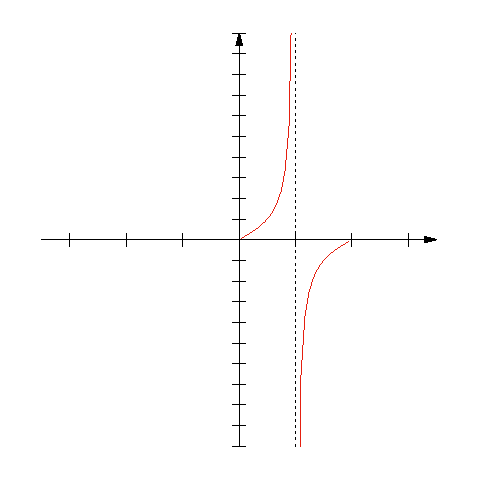
\includegraphics[width={216.00bp},height={216.00bp}]{figura_01_08}}%
    \gplfronttext
  \end{picture}%
\endgroup

\end{figure}
\begin{equation*}
    \int_0^\pi|\tan(t)|\,dt\rightarrow\infty
\end{equation*}
\begin{equation*}
    t=\frac{\pi}{2}:|\tan(t)|\rightarrow\infty
\end{equation*}
\\
\begin{equation*}
    \therefore\,\text{Esta función no tiene serie de \emph{Fourier}.}
\end{equation*}

\section{Evaluación de los coeficientes de \emph{Fourier}}
\begin{equation*}
    f(t)=\frac{a_0}{2}+
    \sum_{n=1}^{\infty}[a_n\cos(n\omega_0\,t)+b_n\sen(n\omega_0\,t)]
\end{equation*}

Integrando ambas partes:
\begin{equation*}
\begin{split}
    \int_{0}^{T}f(t)\,dt
        &=\int_{0}^{T}\frac{a_0}{2}\,dt+
          \sum_{n=1}^{\infty}\left[\int_{0}^{T}a_n\cos(n\omega_0\,t)\,dt+
          \int_{0}^{T}b_n\sen(n\omega_0\,t)\,dt\right]\\
        &=\frac{a_0}{2}t\Biggr|_{0}^{T}\\
        &=\frac{a_0}{2}T\\
\end{split}
\end{equation*}
\begin{equation}
    a_0=\frac{2}{T}\int_{0}^{T}f(t)\,dt
\end{equation}

Para calcular ``$a_n$'' multiplicamos por $\cos(m\omega_0\,t);m\in\mathbb{N}$ e
integramos en 1 periodo.
\begin{equation*}
\begin{split}
    \int_{0}^{T}f(t)\cos(m\omega_0\,t)\,dt
        &=\int_{0}^{T}\frac{a_0}{2}\cos(m\omega_0\,t)\,dt\\
        &+\sum_{n=1}^{\infty}\left[
          \int_{0}^{T}a_n\cos(n\omega_0\,t)\cos(m\omega_0\,t)\,dt+
          \int_{0}^{T}b_n\sen(n\omega_0\,t)\cos(m\omega_0\,t)\,dt\right]\\
        &=0+\sum_{n=1}^{\infty}\left[
          \int_{0}^{T}a_n\cos(n\omega_0\,t)\cos(m\omega_0\,t)\,dt+0\right]\\
\end{split}
\end{equation*}

Para $n\neq m$ todos los elementos de la sumatoria serán igual a $0$.
Por tanto:
\begin{equation*}
\begin{split}
    \int_{0}^{T}f(t)\cos(n\omega_0\,t)\,dt
        &=\int_{0}^{T}a_n\cos^2(n\omega_0\,t)\,dt\\
        &=a_n\frac{T}{2}\\
\end{split}
\end{equation*}
\begin{equation}
    a_n=\frac{2}{T}\int_{0}^{T}f(t)\cos(n\omega_0\,t)\,dt
\end{equation}

Para calcular ``$b_n$'' multiplicamos por $\sen(m\omega_0\,t);m\in\mathbb{N}$ e
integramos en 1 periodo.
\begin{equation*}
\begin{split}
    \int_{0}^{T}f(t)\sen(m\omega_0\,t)\,dt
        &=\int_{0}^{T}\frac{a_0}{2}\sen(m\omega_0\,t)\,dt\\
        &+\sum_{n=1}^{\infty}\left[
          \int_{0}^{T}a_n\cos(n\omega_0\,t)\sen(m\omega_0\,t)\,dt+
          \int_{0}^{T}b_n\sen(n\omega_0\,t)\sen(m\omega_0\,t)\,dt\right]\\
        &=0+\sum_{n=1}^{\infty}\left[
          0+\int_{0}^{T}b_n\sen(n\omega_0\,t)\sen(m\omega_0\,t)\,dt\right]\\
\end{split}
\end{equation*}

Para $n\neq\,m$ todos los elementos de la sumatoria serán igual a $0$.
Por tanto:
\begin{equation*}
\begin{split}
    \int_{0}^{T}f(t)\sen(n\omega_0\,t)\,dt
        &=\int_{0}^{T}b_n\sen^2(n\omega_0\,t)\,dt\\
        &=b_n\,\frac{T}{2}\\
\end{split}
\end{equation*}
\begin{equation}
    b_n=\frac{2}{T}\int_{0}^{T}f(t)\sen(n\omega_0\,t)\,dt
\end{equation}

\section{Formulas para las series de \emph{Fourier}}
\begin{equation*}
    \sen(\pi\,n)=0;\quad\,n\in\mathbb{N}
\end{equation*}
\begin{equation*}
    \cos(\pi\,n)={(-1)}^n;\quad\,n\in\mathbb{N}
\end{equation*}
\begin{equation*}
    \sen(2\pi\,n)=0;\quad\,n\in\mathbb{N}
\end{equation*}
\begin{equation*}
    \cos(2\pi\,n)=1;\quad\,n\in\mathbb{N}
\end{equation*}
\begin{equation*}
    \int\,\sen(at)\,dt=-\frac{\cos(at)}{a}
\end{equation*}
\begin{equation*}
    \int\,\cos(at)\,dt=\frac{\sen(at)}{a}
\end{equation*}
\begin{equation*}
    \int\,t\sen(at)\,dt=-\frac{t}{a}\cos(at)+\frac{1}{a^2}\sen(at)
\end{equation*}
\begin{equation*}
    \int\,t\cos(at)\,dt=\frac{t}{a}\sen(at)+\frac{1}{a^2}\cos(at)
\end{equation*}
\begin{equation*}
    \int\,{e}^{at}\,dt=\frac{1}{a}e^{at}
\end{equation*}
\begin{equation*}
    \int\,t\,{e}^{at}\,dt=\frac{t}{a}\,{e}^{at}-\frac{1}{a^2}{e}^{at}
\end{equation*}


\chapter{Análisis de formas de onda periódica}

\section{Funciones pares e impares}
Una función es \textbf{par} si:
\begin{equation}
    f(-t)=f(t)
\end{equation}
\begin{figure}[H]
    \centering
    % GNUPLOT: LaTeX picture with Postscript
\begingroup
  \makeatletter
  \providecommand\color[2][]{%
    \GenericError{(gnuplot) \space\space\space\@spaces}{%
      Package color not loaded in conjunction with
      terminal option `colourtext'%
    }{See the gnuplot documentation for explanation.%
    }{Either use 'blacktext' in gnuplot or load the package
      color.sty in LaTeX.}%
    \renewcommand\color[2][]{}%
  }%
  \providecommand\includegraphics[2][]{%
    \GenericError{(gnuplot) \space\space\space\@spaces}{%
      Package graphicx or graphics not loaded%
    }{See the gnuplot documentation for explanation.%
    }{The gnuplot epslatex terminal needs graphicx.sty or graphics.sty.}%
    \renewcommand\includegraphics[2][]{}%
  }%
  \providecommand\rotatebox[2]{#2}%
  \@ifundefined{ifGPcolor}{%
    \newif\ifGPcolor
    \GPcolorfalse
  }{}%
  \@ifundefined{ifGPblacktext}{%
    \newif\ifGPblacktext
    \GPblacktexttrue
  }{}%
  % define a \g@addto@macro without @ in the name:
  \let\gplgaddtomacro\g@addto@macro
  % define empty templates for all commands taking text:
  \gdef\gplbacktext{}%
  \gdef\gplfronttext{}%
  \makeatother
  \ifGPblacktext
    % no textcolor at all
    \def\colorrgb#1{}%
    \def\colorgray#1{}%
  \else
    % gray or color?
    \ifGPcolor
      \def\colorrgb#1{\color[rgb]{#1}}%
      \def\colorgray#1{\color[gray]{#1}}%
      \expandafter\def\csname LTw\endcsname{\color{white}}%
      \expandafter\def\csname LTb\endcsname{\color{black}}%
      \expandafter\def\csname LTa\endcsname{\color{black}}%
      \expandafter\def\csname LT0\endcsname{\color[rgb]{1,0,0}}%
      \expandafter\def\csname LT1\endcsname{\color[rgb]{0,1,0}}%
      \expandafter\def\csname LT2\endcsname{\color[rgb]{0,0,1}}%
      \expandafter\def\csname LT3\endcsname{\color[rgb]{1,0,1}}%
      \expandafter\def\csname LT4\endcsname{\color[rgb]{0,1,1}}%
      \expandafter\def\csname LT5\endcsname{\color[rgb]{1,1,0}}%
      \expandafter\def\csname LT6\endcsname{\color[rgb]{0,0,0}}%
      \expandafter\def\csname LT7\endcsname{\color[rgb]{1,0.3,0}}%
      \expandafter\def\csname LT8\endcsname{\color[rgb]{0.5,0.5,0.5}}%
    \else
      % gray
      \def\colorrgb#1{\color{black}}%
      \def\colorgray#1{\color[gray]{#1}}%
      \expandafter\def\csname LTw\endcsname{\color{white}}%
      \expandafter\def\csname LTb\endcsname{\color{black}}%
      \expandafter\def\csname LTa\endcsname{\color{black}}%
      \expandafter\def\csname LT0\endcsname{\color{black}}%
      \expandafter\def\csname LT1\endcsname{\color{black}}%
      \expandafter\def\csname LT2\endcsname{\color{black}}%
      \expandafter\def\csname LT3\endcsname{\color{black}}%
      \expandafter\def\csname LT4\endcsname{\color{black}}%
      \expandafter\def\csname LT5\endcsname{\color{black}}%
      \expandafter\def\csname LT6\endcsname{\color{black}}%
      \expandafter\def\csname LT7\endcsname{\color{black}}%
      \expandafter\def\csname LT8\endcsname{\color{black}}%
    \fi
  \fi
    \setlength{\unitlength}{0.0500bp}%
    \ifx\gptboxheight\undefined%
      \newlength{\gptboxheight}%
      \newlength{\gptboxwidth}%
      \newsavebox{\gptboxtext}%
    \fi%
    \setlength{\fboxrule}{0.5pt}%
    \setlength{\fboxsep}{1pt}%
    \definecolor{tbcol}{rgb}{1,1,1}%
\begin{picture}(4320.00,2880.00)%
    \gplgaddtomacro\gplbacktext{%
      \csname LTb\endcsname%%
      \put(2040,192){\makebox(0,0)[r]{\strut{}}}%
      \put(2040,824){\makebox(0,0)[r]{\strut{}}}%
      \put(2040,1456){\makebox(0,0)[r]{\strut{}}}%
      \put(2040,2087){\makebox(0,0)[r]{\strut{}}}%
      \put(2040,2719){\makebox(0,0)[r]{\strut{}}}%
      \put(240,601){\makebox(0,0){\strut{}}}%
      \put(714,601){\makebox(0,0){\strut{}}}%
      \put(1188,601){\makebox(0,0){\strut{}}}%
      \put(1662,601){\makebox(0,0){\strut{}}}%
      \put(2136,601){\makebox(0,0){\strut{}}}%
      \put(2609,601){\makebox(0,0){\strut{}}}%
      \put(3083,601){\makebox(0,0){\strut{}}}%
      \put(3557,601){\makebox(0,0){\strut{}}}%
      \put(4031,601){\makebox(0,0){\strut{}}}%
      \csname LTb\endcsname%%
      \put(4647,824){\makebox(0,0)[l]{\strut{}$t$}}%
      \put(2349,2972){\makebox(0,0)[l]{\strut{}$f(t)$}}%
      \put(998,634){\makebox(0,0)[l]{\strut{}$-t_1$}}%
      \put(3036,634){\makebox(0,0)[l]{\strut{}$ t_1$}}%
      \put(3320,1771){\makebox(0,0)[l]{\strut{}$f(t_1)=f(-t_1)$}}%
    }%
    \gplgaddtomacro\gplfronttext{%
    }%
    \gplbacktext
    \put(0,0){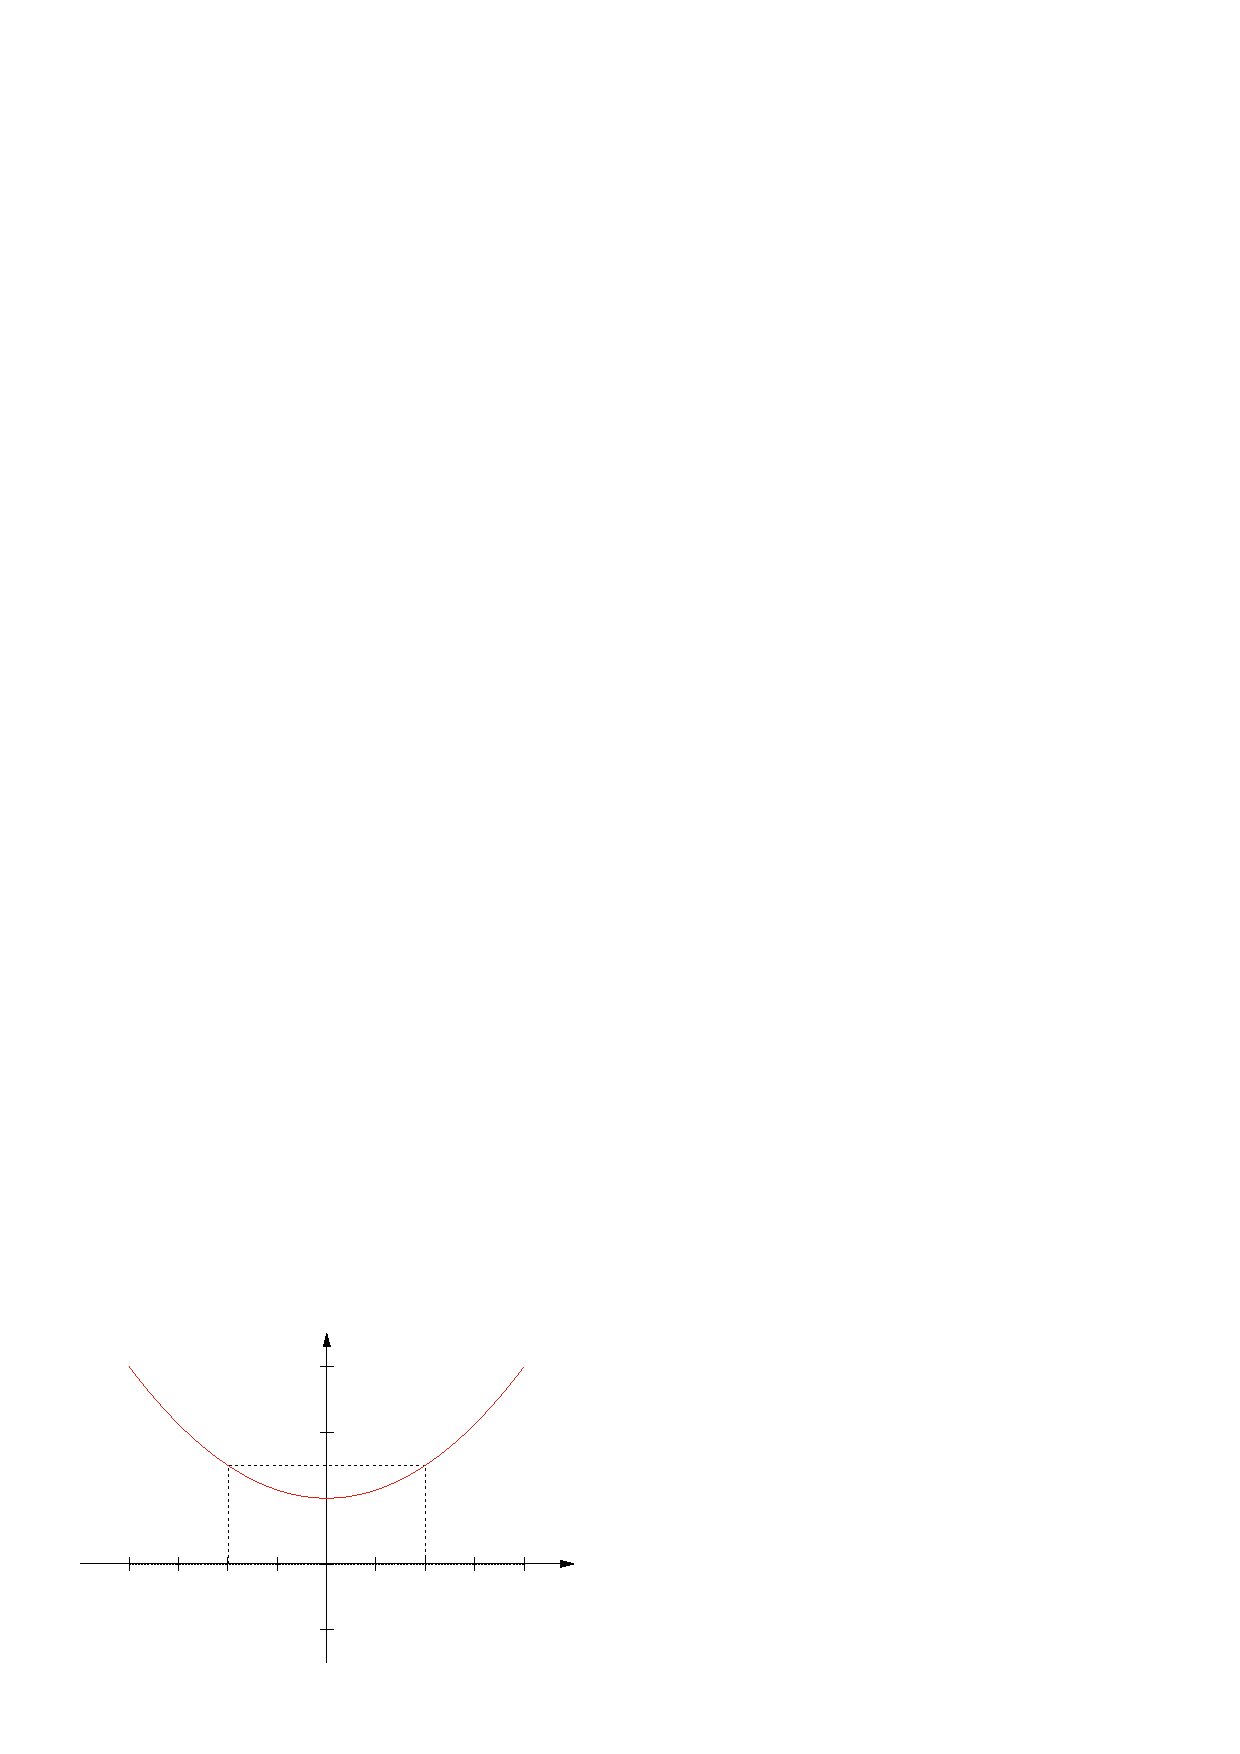
\includegraphics[width={216.00bp},height={144.00bp}]{figura_02_01}}%
    \gplfronttext
  \end{picture}%
\endgroup

    \caption{La gráfica se refleja \\respecto al eje central.}
\end{figure}

\textbf{Ejemplo 1:}
\begin{equation*}
    f(t)=t^2
\end{equation*}
\begin{equation*}
    f(-t)={(-t)}^2=t^2=f(t)
\end{equation*}

\textbf{Ejemplo 2:}
\begin{equation*}
    f(t)=\cos(t)
\end{equation*}
\begin{equation*}
    f(t)=\cos(-t)=\cos(t)=f(t)
\end{equation*}

Una función es \textbf{impar} si:
\begin{equation}
    f(-t)=-f(t)
\end{equation}
\begin{figure}[H]
    \centering
    % GNUPLOT: LaTeX picture with Postscript
\begingroup
  \makeatletter
  \providecommand\color[2][]{%
    \GenericError{(gnuplot) \space\space\space\@spaces}{%
      Package color not loaded in conjunction with
      terminal option `colourtext'%
    }{See the gnuplot documentation for explanation.%
    }{Either use 'blacktext' in gnuplot or load the package
      color.sty in LaTeX.}%
    \renewcommand\color[2][]{}%
  }%
  \providecommand\includegraphics[2][]{%
    \GenericError{(gnuplot) \space\space\space\@spaces}{%
      Package graphicx or graphics not loaded%
    }{See the gnuplot documentation for explanation.%
    }{The gnuplot epslatex terminal needs graphicx.sty or graphics.sty.}%
    \renewcommand\includegraphics[2][]{}%
  }%
  \providecommand\rotatebox[2]{#2}%
  \@ifundefined{ifGPcolor}{%
    \newif\ifGPcolor
    \GPcolorfalse
  }{}%
  \@ifundefined{ifGPblacktext}{%
    \newif\ifGPblacktext
    \GPblacktexttrue
  }{}%
  % define a \g@addto@macro without @ in the name:
  \let\gplgaddtomacro\g@addto@macro
  % define empty templates for all commands taking text:
  \gdef\gplbacktext{}%
  \gdef\gplfronttext{}%
  \makeatother
  \ifGPblacktext
    % no textcolor at all
    \def\colorrgb#1{}%
    \def\colorgray#1{}%
  \else
    % gray or color?
    \ifGPcolor
      \def\colorrgb#1{\color[rgb]{#1}}%
      \def\colorgray#1{\color[gray]{#1}}%
      \expandafter\def\csname LTw\endcsname{\color{white}}%
      \expandafter\def\csname LTb\endcsname{\color{black}}%
      \expandafter\def\csname LTa\endcsname{\color{black}}%
      \expandafter\def\csname LT0\endcsname{\color[rgb]{1,0,0}}%
      \expandafter\def\csname LT1\endcsname{\color[rgb]{0,1,0}}%
      \expandafter\def\csname LT2\endcsname{\color[rgb]{0,0,1}}%
      \expandafter\def\csname LT3\endcsname{\color[rgb]{1,0,1}}%
      \expandafter\def\csname LT4\endcsname{\color[rgb]{0,1,1}}%
      \expandafter\def\csname LT5\endcsname{\color[rgb]{1,1,0}}%
      \expandafter\def\csname LT6\endcsname{\color[rgb]{0,0,0}}%
      \expandafter\def\csname LT7\endcsname{\color[rgb]{1,0.3,0}}%
      \expandafter\def\csname LT8\endcsname{\color[rgb]{0.5,0.5,0.5}}%
    \else
      % gray
      \def\colorrgb#1{\color{black}}%
      \def\colorgray#1{\color[gray]{#1}}%
      \expandafter\def\csname LTw\endcsname{\color{white}}%
      \expandafter\def\csname LTb\endcsname{\color{black}}%
      \expandafter\def\csname LTa\endcsname{\color{black}}%
      \expandafter\def\csname LT0\endcsname{\color{black}}%
      \expandafter\def\csname LT1\endcsname{\color{black}}%
      \expandafter\def\csname LT2\endcsname{\color{black}}%
      \expandafter\def\csname LT3\endcsname{\color{black}}%
      \expandafter\def\csname LT4\endcsname{\color{black}}%
      \expandafter\def\csname LT5\endcsname{\color{black}}%
      \expandafter\def\csname LT6\endcsname{\color{black}}%
      \expandafter\def\csname LT7\endcsname{\color{black}}%
      \expandafter\def\csname LT8\endcsname{\color{black}}%
    \fi
  \fi
    \setlength{\unitlength}{0.0500bp}%
    \ifx\gptboxheight\undefined%
      \newlength{\gptboxheight}%
      \newlength{\gptboxwidth}%
      \newsavebox{\gptboxtext}%
    \fi%
    \setlength{\fboxrule}{0.5pt}%
    \setlength{\fboxsep}{1pt}%
    \definecolor{tbcol}{rgb}{1,1,1}%
\begin{picture}(4320.00,2880.00)%
    \gplgaddtomacro\gplbacktext{%
      \csname LTb\endcsname%%
      \put(2040,192){\makebox(0,0)[r]{\strut{}}}%
      \put(2040,824){\makebox(0,0)[r]{\strut{}}}%
      \put(2040,1456){\makebox(0,0)[r]{\strut{}}}%
      \put(2040,2087){\makebox(0,0)[r]{\strut{}}}%
      \put(2040,2719){\makebox(0,0)[r]{\strut{}}}%
      \put(240,1233){\makebox(0,0){\strut{}}}%
      \put(714,1233){\makebox(0,0){\strut{}}}%
      \put(1188,1233){\makebox(0,0){\strut{}}}%
      \put(1662,1233){\makebox(0,0){\strut{}}}%
      \put(2136,1233){\makebox(0,0){\strut{}}}%
      \put(2609,1233){\makebox(0,0){\strut{}}}%
      \put(3083,1233){\makebox(0,0){\strut{}}}%
      \put(3557,1233){\makebox(0,0){\strut{}}}%
      \put(4031,1233){\makebox(0,0){\strut{}}}%
      \csname LTb\endcsname%%
      \put(4647,1456){\makebox(0,0)[l]{\strut{}$t$}}%
      \put(2349,2845){\makebox(0,0)[l]{\strut{}$f(t)$}}%
      \put(998,1645){\makebox(0,0)[l]{\strut{}$-t_1$}}%
      \put(3036,1266){\makebox(0,0)[l]{\strut{}$ t_1$}}%
      \put(2372,824){\makebox(0,0)[l]{\strut{}$-f(t_1)=f(-t_1)$}}%
    }%
    \gplgaddtomacro\gplfronttext{%
    }%
    \gplbacktext
    \put(0,0){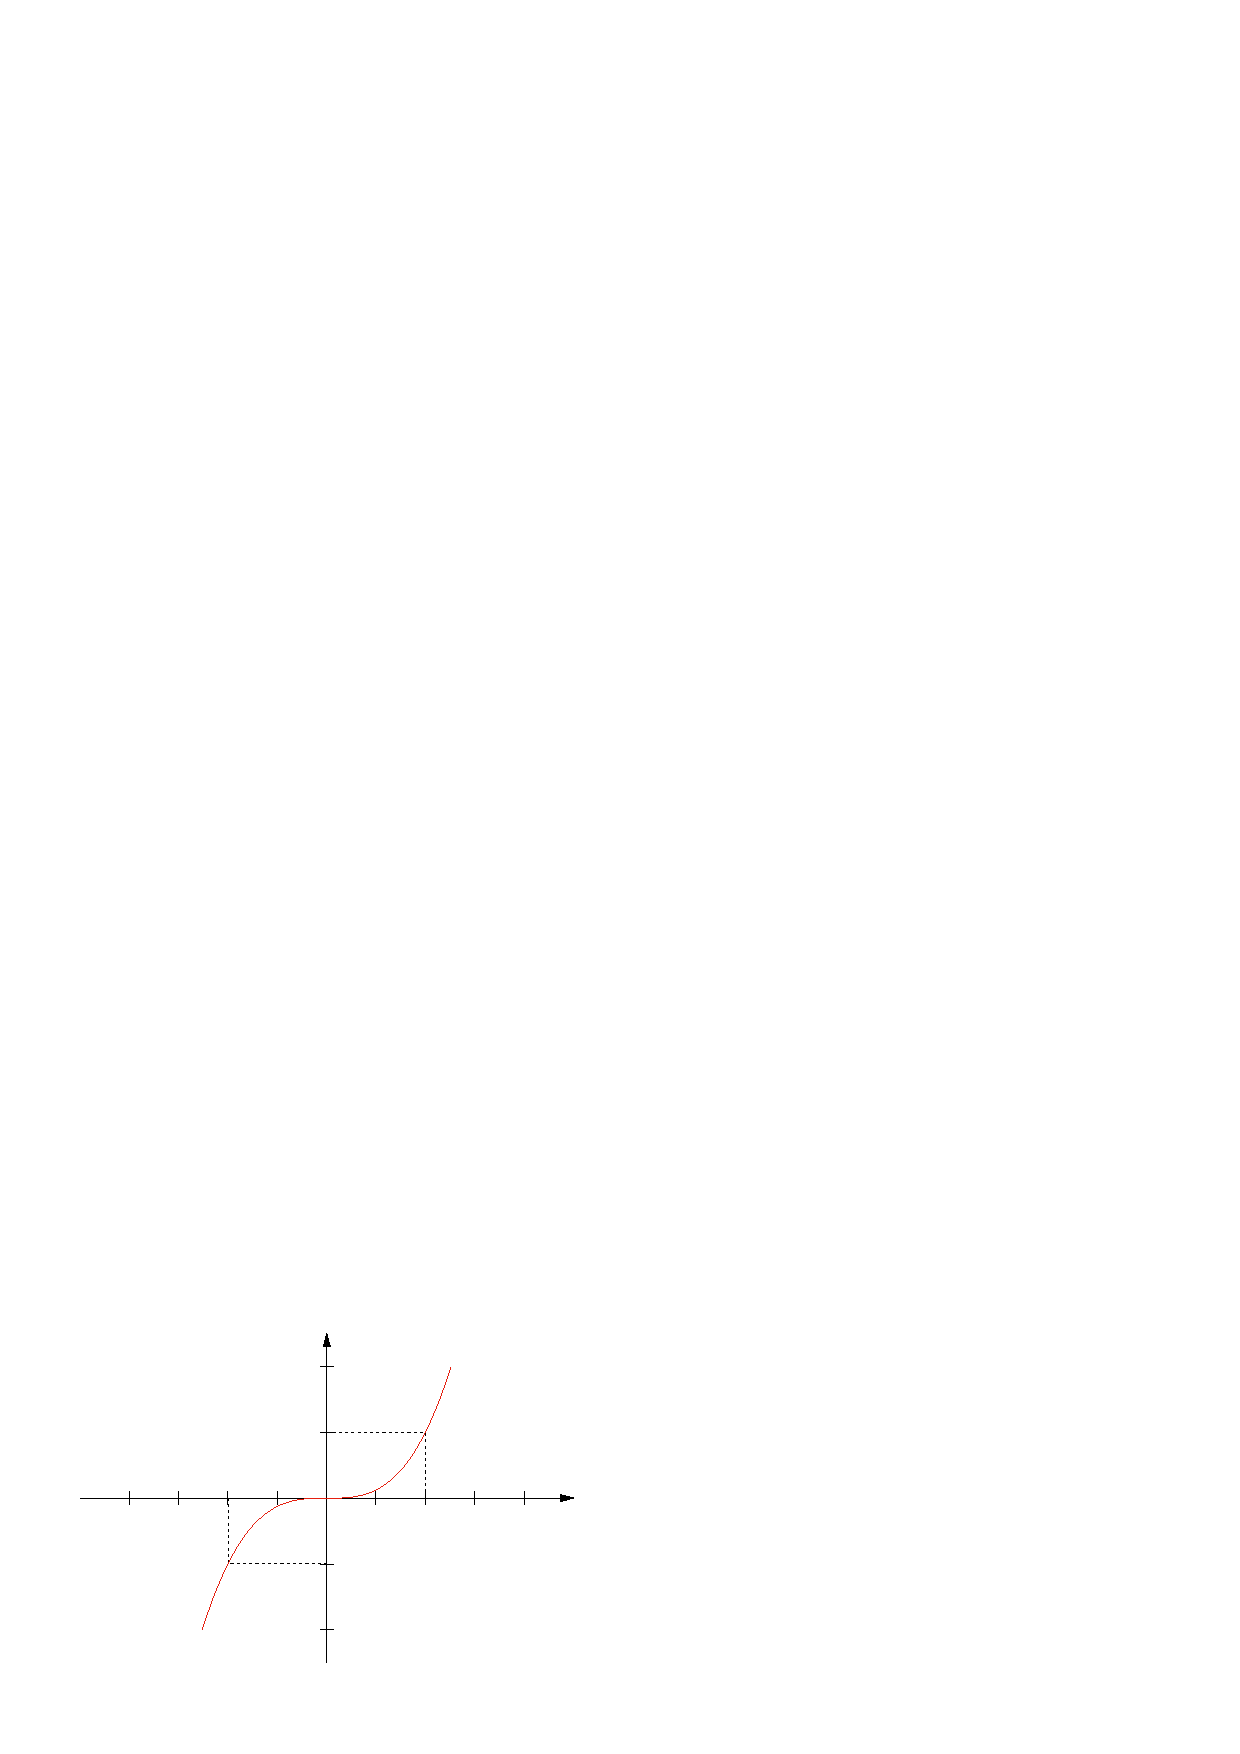
\includegraphics[width={216.00bp},height={144.00bp}]{figura_02_02}}%
    \gplfronttext
  \end{picture}%
\endgroup

    \caption{La gráfica se refleja \\
    1ro respecto al eje central\\
    2do respecto al eje horizontal.}
\end{figure}

\textbf{Ejemplo 3:}
\begin{equation*}
    f(t)=t^3
\end{equation*}
\begin{equation*}
    f(-t)={(-t)}^3=-t^3=-f(t)
\end{equation*}

\textbf{Ejemplo 4:}
\begin{equation*}
    f(t)=\sen(t)
\end{equation*}
\begin{equation*}
    f(t)=\sen(-t)=-\sen(t)=-f(t)
\end{equation*}

\textbf{Ejemplo 5:}
\begin{equation*}
    f(t)=\begin{cases}
        e^t&t<0\\
        e^{-t}&t>0\\
    \end{cases}
\end{equation*}
\begin{equation*}
    f(-t)=\left\{\!\begin{aligned}
    &e^{-t}&-t<0\rightarrow\,t>0\\
    &e^{t}&-t>0\rightarrow\,t<0\\
    \end{aligned}\right\}
    =f(t)
\end{equation*}
\begin{figure}[H]
    \centering
    % GNUPLOT: LaTeX picture with Postscript
\begingroup
  \makeatletter
  \providecommand\color[2][]{%
    \GenericError{(gnuplot) \space\space\space\@spaces}{%
      Package color not loaded in conjunction with
      terminal option `colourtext'%
    }{See the gnuplot documentation for explanation.%
    }{Either use 'blacktext' in gnuplot or load the package
      color.sty in LaTeX.}%
    \renewcommand\color[2][]{}%
  }%
  \providecommand\includegraphics[2][]{%
    \GenericError{(gnuplot) \space\space\space\@spaces}{%
      Package graphicx or graphics not loaded%
    }{See the gnuplot documentation for explanation.%
    }{The gnuplot epslatex terminal needs graphicx.sty or graphics.sty.}%
    \renewcommand\includegraphics[2][]{}%
  }%
  \providecommand\rotatebox[2]{#2}%
  \@ifundefined{ifGPcolor}{%
    \newif\ifGPcolor
    \GPcolorfalse
  }{}%
  \@ifundefined{ifGPblacktext}{%
    \newif\ifGPblacktext
    \GPblacktexttrue
  }{}%
  % define a \g@addto@macro without @ in the name:
  \let\gplgaddtomacro\g@addto@macro
  % define empty templates for all commands taking text:
  \gdef\gplbacktext{}%
  \gdef\gplfronttext{}%
  \makeatother
  \ifGPblacktext
    % no textcolor at all
    \def\colorrgb#1{}%
    \def\colorgray#1{}%
  \else
    % gray or color?
    \ifGPcolor
      \def\colorrgb#1{\color[rgb]{#1}}%
      \def\colorgray#1{\color[gray]{#1}}%
      \expandafter\def\csname LTw\endcsname{\color{white}}%
      \expandafter\def\csname LTb\endcsname{\color{black}}%
      \expandafter\def\csname LTa\endcsname{\color{black}}%
      \expandafter\def\csname LT0\endcsname{\color[rgb]{1,0,0}}%
      \expandafter\def\csname LT1\endcsname{\color[rgb]{0,1,0}}%
      \expandafter\def\csname LT2\endcsname{\color[rgb]{0,0,1}}%
      \expandafter\def\csname LT3\endcsname{\color[rgb]{1,0,1}}%
      \expandafter\def\csname LT4\endcsname{\color[rgb]{0,1,1}}%
      \expandafter\def\csname LT5\endcsname{\color[rgb]{1,1,0}}%
      \expandafter\def\csname LT6\endcsname{\color[rgb]{0,0,0}}%
      \expandafter\def\csname LT7\endcsname{\color[rgb]{1,0.3,0}}%
      \expandafter\def\csname LT8\endcsname{\color[rgb]{0.5,0.5,0.5}}%
    \else
      % gray
      \def\colorrgb#1{\color{black}}%
      \def\colorgray#1{\color[gray]{#1}}%
      \expandafter\def\csname LTw\endcsname{\color{white}}%
      \expandafter\def\csname LTb\endcsname{\color{black}}%
      \expandafter\def\csname LTa\endcsname{\color{black}}%
      \expandafter\def\csname LT0\endcsname{\color{black}}%
      \expandafter\def\csname LT1\endcsname{\color{black}}%
      \expandafter\def\csname LT2\endcsname{\color{black}}%
      \expandafter\def\csname LT3\endcsname{\color{black}}%
      \expandafter\def\csname LT4\endcsname{\color{black}}%
      \expandafter\def\csname LT5\endcsname{\color{black}}%
      \expandafter\def\csname LT6\endcsname{\color{black}}%
      \expandafter\def\csname LT7\endcsname{\color{black}}%
      \expandafter\def\csname LT8\endcsname{\color{black}}%
    \fi
  \fi
    \setlength{\unitlength}{0.0500bp}%
    \ifx\gptboxheight\undefined%
      \newlength{\gptboxheight}%
      \newlength{\gptboxwidth}%
      \newsavebox{\gptboxtext}%
    \fi%
    \setlength{\fboxrule}{0.5pt}%
    \setlength{\fboxsep}{1pt}%
    \definecolor{tbcol}{rgb}{1,1,1}%
\begin{picture}(5760.00,1440.00)%
    \gplgaddtomacro\gplbacktext{%
      \csname LTb\endcsname%%
      \put(2760,464){\makebox(0,0)[r]{\strut{}}}%
      \put(2760,1007){\makebox(0,0)[r]{\strut{}}}%
      \put(240,241){\makebox(0,0){\strut{}}}%
      \put(763,241){\makebox(0,0){\strut{}}}%
      \put(1286,241){\makebox(0,0){\strut{}}}%
      \put(1809,241){\makebox(0,0){\strut{}}}%
      \put(2332,241){\makebox(0,0){\strut{}}}%
      \put(2856,241){\makebox(0,0){\strut{}}}%
      \put(3379,241){\makebox(0,0){\strut{}}}%
      \put(3902,241){\makebox(0,0){\strut{}}}%
      \put(4425,241){\makebox(0,0){\strut{}}}%
      \put(4948,241){\makebox(0,0){\strut{}}}%
      \put(5471,241){\makebox(0,0){\strut{}}}%
      \csname LTb\endcsname%%
      \put(6256,464){\makebox(0,0)[l]{\strut{}$t$}}%
      \put(2751,1496){\makebox(0,0)[l]{\strut{}$f(t)$}}%
    }%
    \gplgaddtomacro\gplfronttext{%
    }%
    \gplgaddtomacro\gplbacktext{%
      \csname LTb\endcsname%%
      \put(2760,464){\makebox(0,0)[r]{\strut{}}}%
      \put(2760,1007){\makebox(0,0)[r]{\strut{}}}%
      \put(240,241){\makebox(0,0){\strut{}}}%
      \put(763,241){\makebox(0,0){\strut{}}}%
      \put(1286,241){\makebox(0,0){\strut{}}}%
      \put(1809,241){\makebox(0,0){\strut{}}}%
      \put(2332,241){\makebox(0,0){\strut{}}}%
      \put(2856,241){\makebox(0,0){\strut{}}}%
      \put(3379,241){\makebox(0,0){\strut{}}}%
      \put(3902,241){\makebox(0,0){\strut{}}}%
      \put(4425,241){\makebox(0,0){\strut{}}}%
      \put(4948,241){\makebox(0,0){\strut{}}}%
      \put(5471,241){\makebox(0,0){\strut{}}}%
      \csname LTb\endcsname%%
      \put(6256,464){\makebox(0,0)[l]{\strut{}$t$}}%
      \put(2751,1496){\makebox(0,0)[l]{\strut{}$f(t)$}}%
    }%
    \gplgaddtomacro\gplfronttext{%
    }%
    \gplbacktext
    \put(0,0){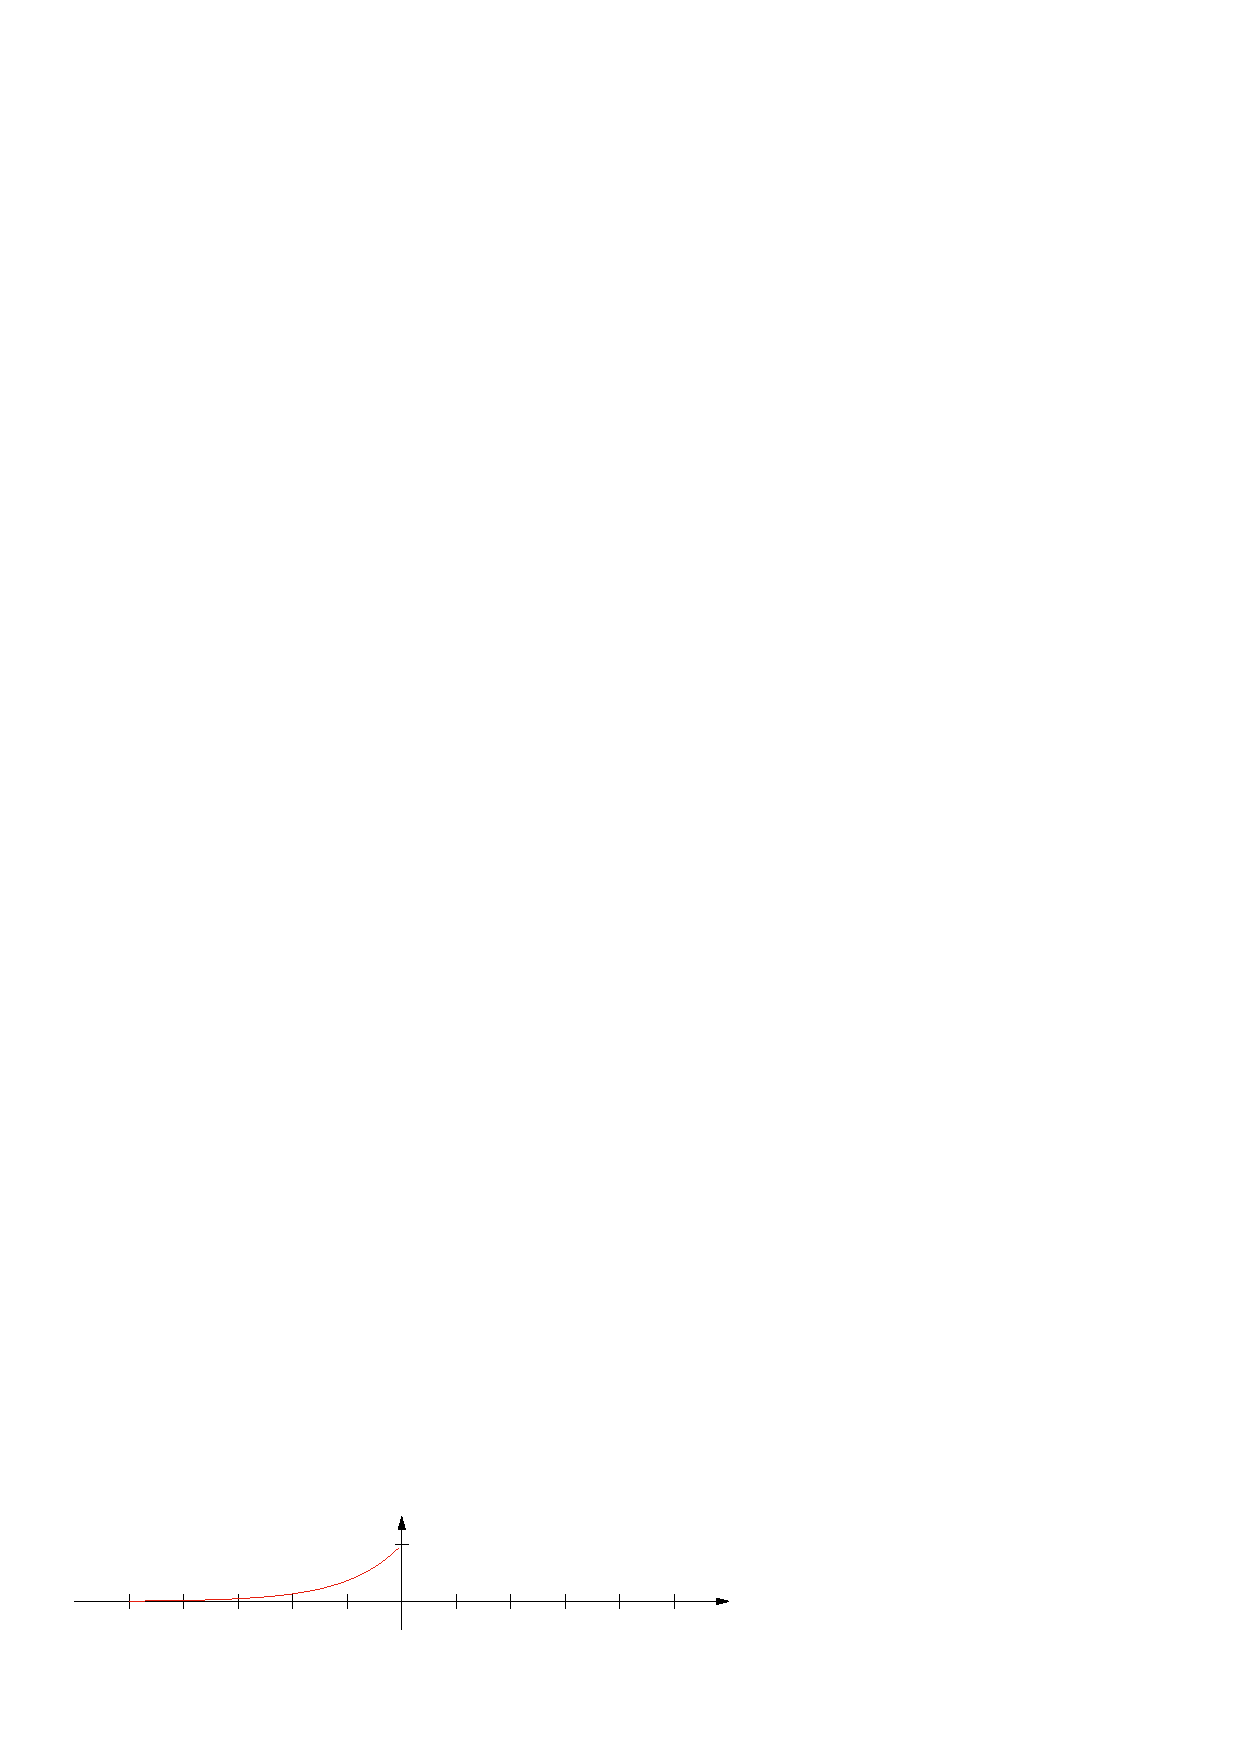
\includegraphics[width={288.00bp},height={72.00bp}]{figura_02_03}}%
    \gplfronttext
  \end{picture}%
\endgroup

\end{figure}

\subsection{Propiedades de las funciones pares e impares}
\subsubsection*{Propiedad 1}
Si $f(t)$ es \textbf{par} y $g(t)$ es \textbf{par}, entonces $h(t)=f(t)g(t)$ es
\textbf{par}.

\underline{Prueba}:
\begin{equation*}
\begin{cases}
    &f(-t)=f(t)\\
    &g(-t)=g(t)\\
\end{cases}
\end{equation*}
\begin{equation*}
\begin{split}
    h(-t)
        &=f(-t)g(-t)\\
        &=f(t)g(t)\\
        &=h(t)\\
\end{split}
\end{equation*}

\subsubsection*{Propiedad 2}
Si $f(t)$ es \textbf{impar} y $g(t)$ es \textbf{impar}, entonces $h(t)=f(t)g(t)$
es \textbf{par}.

\underline{Prueba}:
\begin{equation*}
\begin{cases}
    &f(-t)=-f(t)\\
    &g(-t)=-g(t)\\
\end{cases}
\end{equation*}

\subsubsection*{Propiedad 3}
Si $f(t)$ es \textbf{par} y $g(t)$ es \textbf{impar}, entonces $h(t)=f(t)g(t)$
es \textbf{impar}.

\underline{Prueba}:
\begin{equation*}
\begin{cases}
    &f(-t)=f(t)\\
    &g(-t)=-g(t)\\
\end{cases}
\end{equation*}
\begin{equation*}
\begin{split}
    h(-t)
        &=f(-t)g(-t)\\
        &=f(t)(-g(t))\\
        &=-f(t)g(t)\\
        &=-h(t)\\
\end{split}
\end{equation*}

\subsubsection*{Propiedad 4}
Si $f(t)$ es \textbf{par}, entonces:
\begin{equation}
    \int_{-a}^a\,f(t)\,dt=2\int_0^a\,f(t)\,dt
\end{equation}
\begin{figure}[H]
    \centering
    % GNUPLOT: LaTeX picture with Postscript
\begingroup
  \makeatletter
  \providecommand\color[2][]{%
    \GenericError{(gnuplot) \space\space\space\@spaces}{%
      Package color not loaded in conjunction with
      terminal option `colourtext'%
    }{See the gnuplot documentation for explanation.%
    }{Either use 'blacktext' in gnuplot or load the package
      color.sty in LaTeX.}%
    \renewcommand\color[2][]{}%
  }%
  \providecommand\includegraphics[2][]{%
    \GenericError{(gnuplot) \space\space\space\@spaces}{%
      Package graphicx or graphics not loaded%
    }{See the gnuplot documentation for explanation.%
    }{The gnuplot epslatex terminal needs graphicx.sty or graphics.sty.}%
    \renewcommand\includegraphics[2][]{}%
  }%
  \providecommand\rotatebox[2]{#2}%
  \@ifundefined{ifGPcolor}{%
    \newif\ifGPcolor
    \GPcolorfalse
  }{}%
  \@ifundefined{ifGPblacktext}{%
    \newif\ifGPblacktext
    \GPblacktexttrue
  }{}%
  % define a \g@addto@macro without @ in the name:
  \let\gplgaddtomacro\g@addto@macro
  % define empty templates for all commands taking text:
  \gdef\gplbacktext{}%
  \gdef\gplfronttext{}%
  \makeatother
  \ifGPblacktext
    % no textcolor at all
    \def\colorrgb#1{}%
    \def\colorgray#1{}%
  \else
    % gray or color?
    \ifGPcolor
      \def\colorrgb#1{\color[rgb]{#1}}%
      \def\colorgray#1{\color[gray]{#1}}%
      \expandafter\def\csname LTw\endcsname{\color{white}}%
      \expandafter\def\csname LTb\endcsname{\color{black}}%
      \expandafter\def\csname LTa\endcsname{\color{black}}%
      \expandafter\def\csname LT0\endcsname{\color[rgb]{1,0,0}}%
      \expandafter\def\csname LT1\endcsname{\color[rgb]{0,1,0}}%
      \expandafter\def\csname LT2\endcsname{\color[rgb]{0,0,1}}%
      \expandafter\def\csname LT3\endcsname{\color[rgb]{1,0,1}}%
      \expandafter\def\csname LT4\endcsname{\color[rgb]{0,1,1}}%
      \expandafter\def\csname LT5\endcsname{\color[rgb]{1,1,0}}%
      \expandafter\def\csname LT6\endcsname{\color[rgb]{0,0,0}}%
      \expandafter\def\csname LT7\endcsname{\color[rgb]{1,0.3,0}}%
      \expandafter\def\csname LT8\endcsname{\color[rgb]{0.5,0.5,0.5}}%
    \else
      % gray
      \def\colorrgb#1{\color{black}}%
      \def\colorgray#1{\color[gray]{#1}}%
      \expandafter\def\csname LTw\endcsname{\color{white}}%
      \expandafter\def\csname LTb\endcsname{\color{black}}%
      \expandafter\def\csname LTa\endcsname{\color{black}}%
      \expandafter\def\csname LT0\endcsname{\color{black}}%
      \expandafter\def\csname LT1\endcsname{\color{black}}%
      \expandafter\def\csname LT2\endcsname{\color{black}}%
      \expandafter\def\csname LT3\endcsname{\color{black}}%
      \expandafter\def\csname LT4\endcsname{\color{black}}%
      \expandafter\def\csname LT5\endcsname{\color{black}}%
      \expandafter\def\csname LT6\endcsname{\color{black}}%
      \expandafter\def\csname LT7\endcsname{\color{black}}%
      \expandafter\def\csname LT8\endcsname{\color{black}}%
    \fi
  \fi
    \setlength{\unitlength}{0.0500bp}%
    \ifx\gptboxheight\undefined%
      \newlength{\gptboxheight}%
      \newlength{\gptboxwidth}%
      \newsavebox{\gptboxtext}%
    \fi%
    \setlength{\fboxrule}{0.5pt}%
    \setlength{\fboxsep}{1pt}%
    \definecolor{tbcol}{rgb}{1,1,1}%
\begin{picture}(4320.00,2880.00)%
    \gplgaddtomacro\gplbacktext{%
      \csname LTb\endcsname%%
      \put(2040,192){\makebox(0,0)[r]{\strut{}}}%
      \put(2040,824){\makebox(0,0)[r]{\strut{}}}%
      \put(2040,1456){\makebox(0,0)[r]{\strut{}}}%
      \put(2040,2087){\makebox(0,0)[r]{\strut{}}}%
      \put(2040,2719){\makebox(0,0)[r]{\strut{}}}%
      \put(240,601){\makebox(0,0){\strut{}}}%
      \put(714,601){\makebox(0,0){\strut{}}}%
      \put(1188,601){\makebox(0,0){\strut{}}}%
      \put(1662,601){\makebox(0,0){\strut{}}}%
      \put(2136,601){\makebox(0,0){\strut{}}}%
      \put(2609,601){\makebox(0,0){\strut{}}}%
      \put(3083,601){\makebox(0,0){\strut{}}}%
      \put(3557,601){\makebox(0,0){\strut{}}}%
      \put(4031,601){\makebox(0,0){\strut{}}}%
      \csname LTb\endcsname%%
      \put(4647,824){\makebox(0,0)[l]{\strut{}$t$}}%
      \put(2349,2972){\makebox(0,0)[l]{\strut{}$f(t)$}}%
      \put(998,634){\makebox(0,0)[l]{\strut{}$-a$}}%
      \put(3036,634){\makebox(0,0)[l]{\strut{}$ a$}}%
      \put(3557,1456){\makebox(0,0)[l]{\strut{}$\int_0^a f(t)dt$}}%
    }%
    \gplgaddtomacro\gplfronttext{%
    }%
    \gplgaddtomacro\gplbacktext{%
      \csname LTb\endcsname%%
      \put(2040,192){\makebox(0,0)[r]{\strut{}}}%
      \put(2040,824){\makebox(0,0)[r]{\strut{}}}%
      \put(2040,1456){\makebox(0,0)[r]{\strut{}}}%
      \put(2040,2087){\makebox(0,0)[r]{\strut{}}}%
      \put(2040,2719){\makebox(0,0)[r]{\strut{}}}%
      \put(240,601){\makebox(0,0){\strut{}}}%
      \put(714,601){\makebox(0,0){\strut{}}}%
      \put(1188,601){\makebox(0,0){\strut{}}}%
      \put(1662,601){\makebox(0,0){\strut{}}}%
      \put(2136,601){\makebox(0,0){\strut{}}}%
      \put(2609,601){\makebox(0,0){\strut{}}}%
      \put(3083,601){\makebox(0,0){\strut{}}}%
      \put(3557,601){\makebox(0,0){\strut{}}}%
      \put(4031,601){\makebox(0,0){\strut{}}}%
      \csname LTb\endcsname%%
      \put(4647,824){\makebox(0,0)[l]{\strut{}$t$}}%
      \put(2349,2972){\makebox(0,0)[l]{\strut{}$f(t)$}}%
      \put(998,634){\makebox(0,0)[l]{\strut{}$-a$}}%
      \put(3036,634){\makebox(0,0)[l]{\strut{}$ a$}}%
      \put(3557,1456){\makebox(0,0)[l]{\strut{}$\int_0^a f(t)dt$}}%
    }%
    \gplgaddtomacro\gplfronttext{%
    }%
    \gplgaddtomacro\gplbacktext{%
      \csname LTb\endcsname%%
      \put(2040,192){\makebox(0,0)[r]{\strut{}}}%
      \put(2040,824){\makebox(0,0)[r]{\strut{}}}%
      \put(2040,1456){\makebox(0,0)[r]{\strut{}}}%
      \put(2040,2087){\makebox(0,0)[r]{\strut{}}}%
      \put(2040,2719){\makebox(0,0)[r]{\strut{}}}%
      \put(240,601){\makebox(0,0){\strut{}}}%
      \put(714,601){\makebox(0,0){\strut{}}}%
      \put(1188,601){\makebox(0,0){\strut{}}}%
      \put(1662,601){\makebox(0,0){\strut{}}}%
      \put(2136,601){\makebox(0,0){\strut{}}}%
      \put(2609,601){\makebox(0,0){\strut{}}}%
      \put(3083,601){\makebox(0,0){\strut{}}}%
      \put(3557,601){\makebox(0,0){\strut{}}}%
      \put(4031,601){\makebox(0,0){\strut{}}}%
      \csname LTb\endcsname%%
      \put(4647,824){\makebox(0,0)[l]{\strut{}$t$}}%
      \put(2349,2972){\makebox(0,0)[l]{\strut{}$f(t)$}}%
      \put(998,634){\makebox(0,0)[l]{\strut{}$-a$}}%
      \put(3036,634){\makebox(0,0)[l]{\strut{}$ a$}}%
      \put(3557,1456){\makebox(0,0)[l]{\strut{}$\int_0^a f(t)dt$}}%
    }%
    \gplgaddtomacro\gplfronttext{%
    }%
    \gplbacktext
    \put(0,0){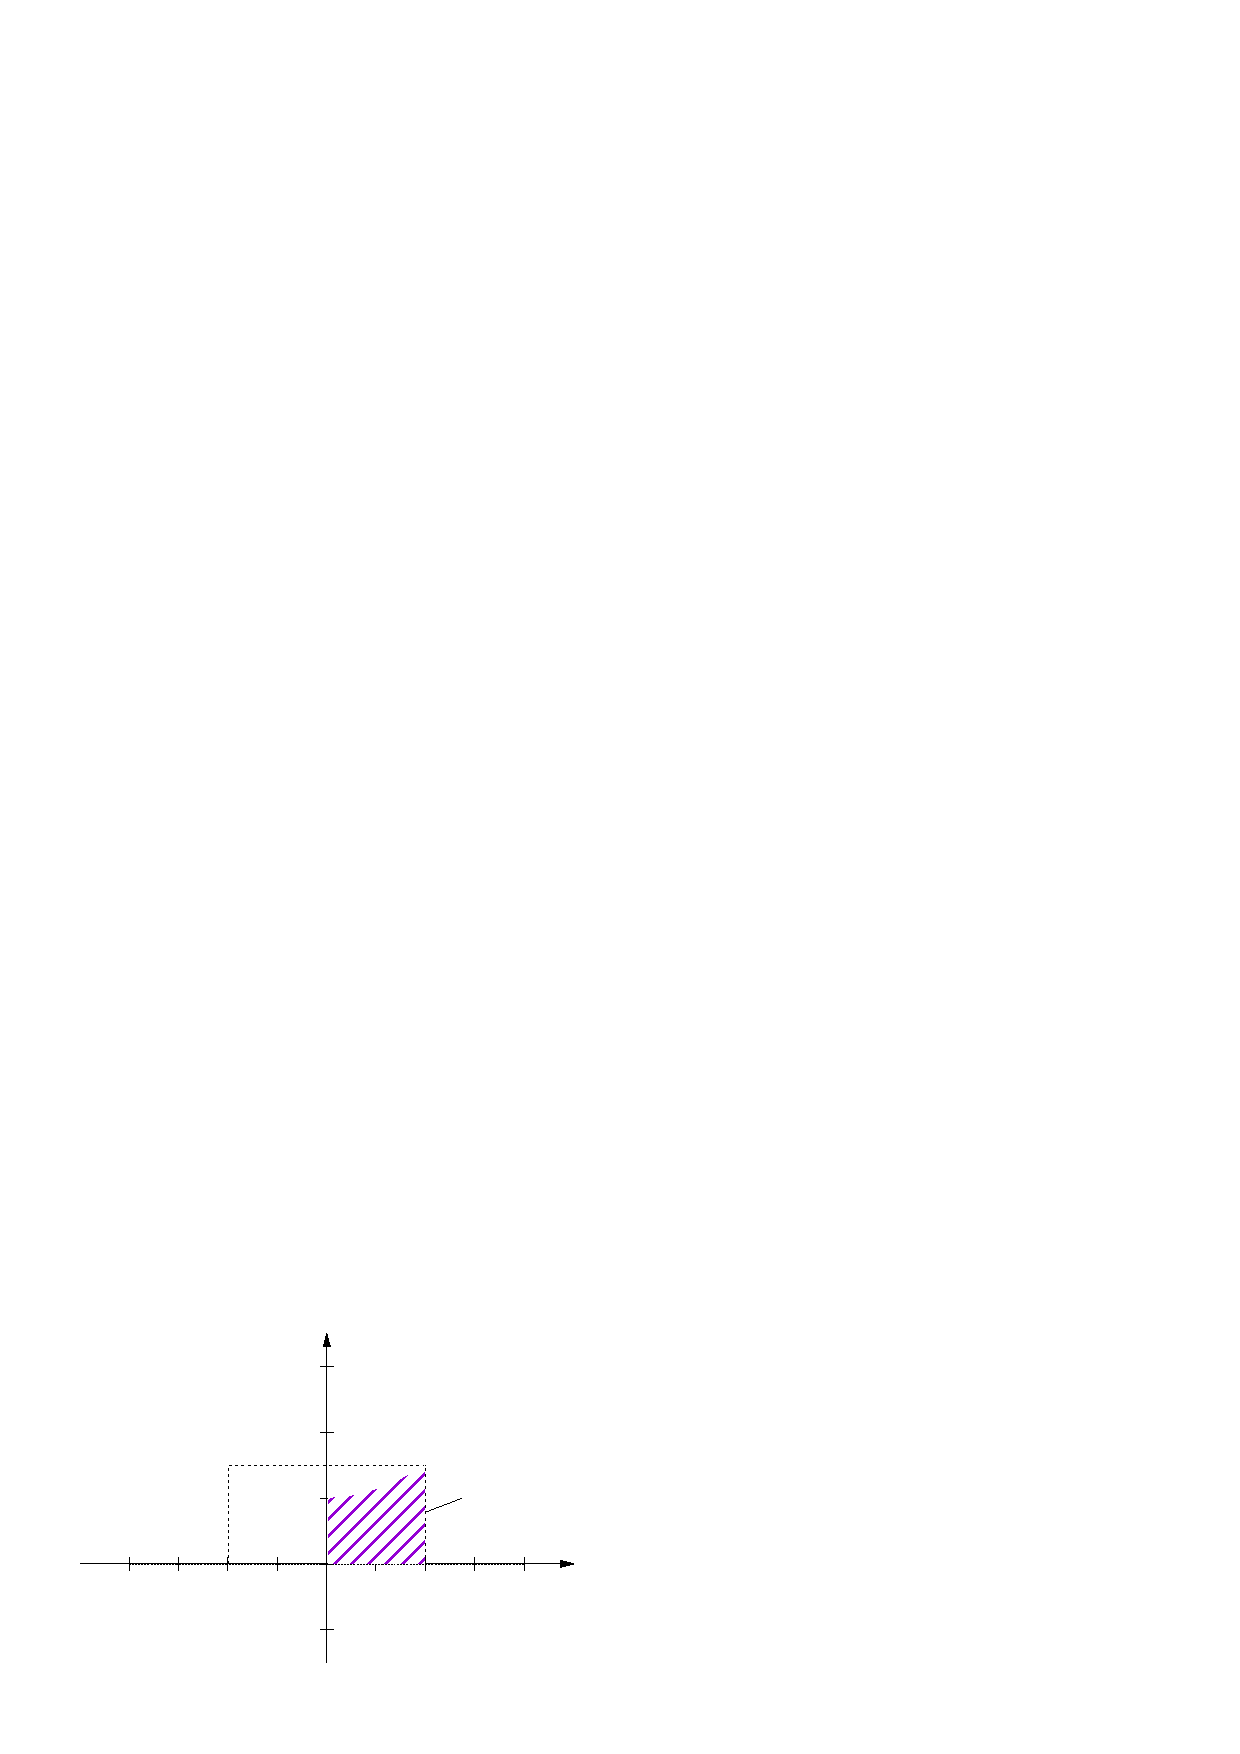
\includegraphics[width={216.00bp},height={144.00bp}]{figura_02_04}}%
    \gplfronttext
  \end{picture}%
\endgroup

\end{figure}

\underline{Prueba}:
\begin{equation*}
\begin{split}
    \int_{-a}^a\,f(t)\,dt
        &=\int_{-a}^0\,f(t)\,dt+\int_0^a\,f(t)\,dt\\
        &=\int_{-a}^0\,f(-t)\,dt+\int_0^a\,f(t)\,dt\\
\end{split}
\end{equation*}
\begin{equation*}
    \tau=-t
\end{equation*}
\begin{equation*}
    d\tau=-dt
\end{equation*}
\begin{equation*}
\begin{split}
    \int_{-a}^a\,f(t)\,dt
        &=\int_a^0\,f(\tau)\,(-d\tau)+\int_0^a\,f(t)\,dt\\
        &=\int_0^a\,f(\tau)\,d\tau+\int_0^a\,f(t)\,dt\\
        &=2\int_0^a\,f(t)\,dt\\
\end{split}
\end{equation*}

\subsubsection*{Propiedad 5}
Si $f(t)$ es \textbf{impar}, entonces:
\begin{equation}
    \int_{-a}^a\,f(t)\,dt=0
\end{equation}
\begin{figure}[H]
    \centering
    % GNUPLOT: LaTeX picture with Postscript
\begingroup
  \makeatletter
  \providecommand\color[2][]{%
    \GenericError{(gnuplot) \space\space\space\@spaces}{%
      Package color not loaded in conjunction with
      terminal option `colourtext'%
    }{See the gnuplot documentation for explanation.%
    }{Either use 'blacktext' in gnuplot or load the package
      color.sty in LaTeX.}%
    \renewcommand\color[2][]{}%
  }%
  \providecommand\includegraphics[2][]{%
    \GenericError{(gnuplot) \space\space\space\@spaces}{%
      Package graphicx or graphics not loaded%
    }{See the gnuplot documentation for explanation.%
    }{The gnuplot epslatex terminal needs graphicx.sty or graphics.sty.}%
    \renewcommand\includegraphics[2][]{}%
  }%
  \providecommand\rotatebox[2]{#2}%
  \@ifundefined{ifGPcolor}{%
    \newif\ifGPcolor
    \GPcolorfalse
  }{}%
  \@ifundefined{ifGPblacktext}{%
    \newif\ifGPblacktext
    \GPblacktexttrue
  }{}%
  % define a \g@addto@macro without @ in the name:
  \let\gplgaddtomacro\g@addto@macro
  % define empty templates for all commands taking text:
  \gdef\gplbacktext{}%
  \gdef\gplfronttext{}%
  \makeatother
  \ifGPblacktext
    % no textcolor at all
    \def\colorrgb#1{}%
    \def\colorgray#1{}%
  \else
    % gray or color?
    \ifGPcolor
      \def\colorrgb#1{\color[rgb]{#1}}%
      \def\colorgray#1{\color[gray]{#1}}%
      \expandafter\def\csname LTw\endcsname{\color{white}}%
      \expandafter\def\csname LTb\endcsname{\color{black}}%
      \expandafter\def\csname LTa\endcsname{\color{black}}%
      \expandafter\def\csname LT0\endcsname{\color[rgb]{1,0,0}}%
      \expandafter\def\csname LT1\endcsname{\color[rgb]{0,1,0}}%
      \expandafter\def\csname LT2\endcsname{\color[rgb]{0,0,1}}%
      \expandafter\def\csname LT3\endcsname{\color[rgb]{1,0,1}}%
      \expandafter\def\csname LT4\endcsname{\color[rgb]{0,1,1}}%
      \expandafter\def\csname LT5\endcsname{\color[rgb]{1,1,0}}%
      \expandafter\def\csname LT6\endcsname{\color[rgb]{0,0,0}}%
      \expandafter\def\csname LT7\endcsname{\color[rgb]{1,0.3,0}}%
      \expandafter\def\csname LT8\endcsname{\color[rgb]{0.5,0.5,0.5}}%
    \else
      % gray
      \def\colorrgb#1{\color{black}}%
      \def\colorgray#1{\color[gray]{#1}}%
      \expandafter\def\csname LTw\endcsname{\color{white}}%
      \expandafter\def\csname LTb\endcsname{\color{black}}%
      \expandafter\def\csname LTa\endcsname{\color{black}}%
      \expandafter\def\csname LT0\endcsname{\color{black}}%
      \expandafter\def\csname LT1\endcsname{\color{black}}%
      \expandafter\def\csname LT2\endcsname{\color{black}}%
      \expandafter\def\csname LT3\endcsname{\color{black}}%
      \expandafter\def\csname LT4\endcsname{\color{black}}%
      \expandafter\def\csname LT5\endcsname{\color{black}}%
      \expandafter\def\csname LT6\endcsname{\color{black}}%
      \expandafter\def\csname LT7\endcsname{\color{black}}%
      \expandafter\def\csname LT8\endcsname{\color{black}}%
    \fi
  \fi
    \setlength{\unitlength}{0.0500bp}%
    \ifx\gptboxheight\undefined%
      \newlength{\gptboxheight}%
      \newlength{\gptboxwidth}%
      \newsavebox{\gptboxtext}%
    \fi%
    \setlength{\fboxrule}{0.5pt}%
    \setlength{\fboxsep}{1pt}%
    \definecolor{tbcol}{rgb}{1,1,1}%
\begin{picture}(4320.00,2880.00)%
    \gplgaddtomacro\gplbacktext{%
      \csname LTb\endcsname%%
      \put(2040,192){\makebox(0,0)[r]{\strut{}}}%
      \put(2040,824){\makebox(0,0)[r]{\strut{}}}%
      \put(2040,1456){\makebox(0,0)[r]{\strut{}}}%
      \put(2040,2087){\makebox(0,0)[r]{\strut{}}}%
      \put(2040,2719){\makebox(0,0)[r]{\strut{}}}%
      \put(240,1233){\makebox(0,0){\strut{}}}%
      \put(714,1233){\makebox(0,0){\strut{}}}%
      \put(1188,1233){\makebox(0,0){\strut{}}}%
      \put(1662,1233){\makebox(0,0){\strut{}}}%
      \put(2136,1233){\makebox(0,0){\strut{}}}%
      \put(2609,1233){\makebox(0,0){\strut{}}}%
      \put(3083,1233){\makebox(0,0){\strut{}}}%
      \put(3557,1233){\makebox(0,0){\strut{}}}%
      \put(4031,1233){\makebox(0,0){\strut{}}}%
      \csname LTb\endcsname%%
      \put(4647,1456){\makebox(0,0)[l]{\strut{}$t$}}%
      \put(2349,2845){\makebox(0,0)[l]{\strut{}$f(t)$}}%
      \put(998,1645){\makebox(0,0)[l]{\strut{}$-a$}}%
      \put(3036,1266){\makebox(0,0)[l]{\strut{}$ a$}}%
      \put(3557,2087){\makebox(0,0)[l]{\strut{}$\int_0^a f(t)dt$}}%
    }%
    \gplgaddtomacro\gplfronttext{%
    }%
    \gplgaddtomacro\gplbacktext{%
      \csname LTb\endcsname%%
      \put(2040,192){\makebox(0,0)[r]{\strut{}}}%
      \put(2040,824){\makebox(0,0)[r]{\strut{}}}%
      \put(2040,1456){\makebox(0,0)[r]{\strut{}}}%
      \put(2040,2087){\makebox(0,0)[r]{\strut{}}}%
      \put(2040,2719){\makebox(0,0)[r]{\strut{}}}%
      \put(240,1233){\makebox(0,0){\strut{}}}%
      \put(714,1233){\makebox(0,0){\strut{}}}%
      \put(1188,1233){\makebox(0,0){\strut{}}}%
      \put(1662,1233){\makebox(0,0){\strut{}}}%
      \put(2136,1233){\makebox(0,0){\strut{}}}%
      \put(2609,1233){\makebox(0,0){\strut{}}}%
      \put(3083,1233){\makebox(0,0){\strut{}}}%
      \put(3557,1233){\makebox(0,0){\strut{}}}%
      \put(4031,1233){\makebox(0,0){\strut{}}}%
      \csname LTb\endcsname%%
      \put(4647,1456){\makebox(0,0)[l]{\strut{}$t$}}%
      \put(2349,2845){\makebox(0,0)[l]{\strut{}$f(t)$}}%
      \put(998,1645){\makebox(0,0)[l]{\strut{}$-a$}}%
      \put(3036,1266){\makebox(0,0)[l]{\strut{}$ a$}}%
      \put(3557,2087){\makebox(0,0)[l]{\strut{}$\int_0^a f(t)dt$}}%
    }%
    \gplgaddtomacro\gplfronttext{%
    }%
    \gplgaddtomacro\gplbacktext{%
      \csname LTb\endcsname%%
      \put(2040,192){\makebox(0,0)[r]{\strut{}}}%
      \put(2040,824){\makebox(0,0)[r]{\strut{}}}%
      \put(2040,1456){\makebox(0,0)[r]{\strut{}}}%
      \put(2040,2087){\makebox(0,0)[r]{\strut{}}}%
      \put(2040,2719){\makebox(0,0)[r]{\strut{}}}%
      \put(240,1233){\makebox(0,0){\strut{}}}%
      \put(714,1233){\makebox(0,0){\strut{}}}%
      \put(1188,1233){\makebox(0,0){\strut{}}}%
      \put(1662,1233){\makebox(0,0){\strut{}}}%
      \put(2136,1233){\makebox(0,0){\strut{}}}%
      \put(2609,1233){\makebox(0,0){\strut{}}}%
      \put(3083,1233){\makebox(0,0){\strut{}}}%
      \put(3557,1233){\makebox(0,0){\strut{}}}%
      \put(4031,1233){\makebox(0,0){\strut{}}}%
      \csname LTb\endcsname%%
      \put(4647,1456){\makebox(0,0)[l]{\strut{}$t$}}%
      \put(2349,2845){\makebox(0,0)[l]{\strut{}$f(t)$}}%
      \put(998,1645){\makebox(0,0)[l]{\strut{}$-a$}}%
      \put(3036,1266){\makebox(0,0)[l]{\strut{}$ a$}}%
      \put(3557,2087){\makebox(0,0)[l]{\strut{}$\int_0^a f(t)dt$}}%
    }%
    \gplgaddtomacro\gplfronttext{%
    }%
    \gplbacktext
    \put(0,0){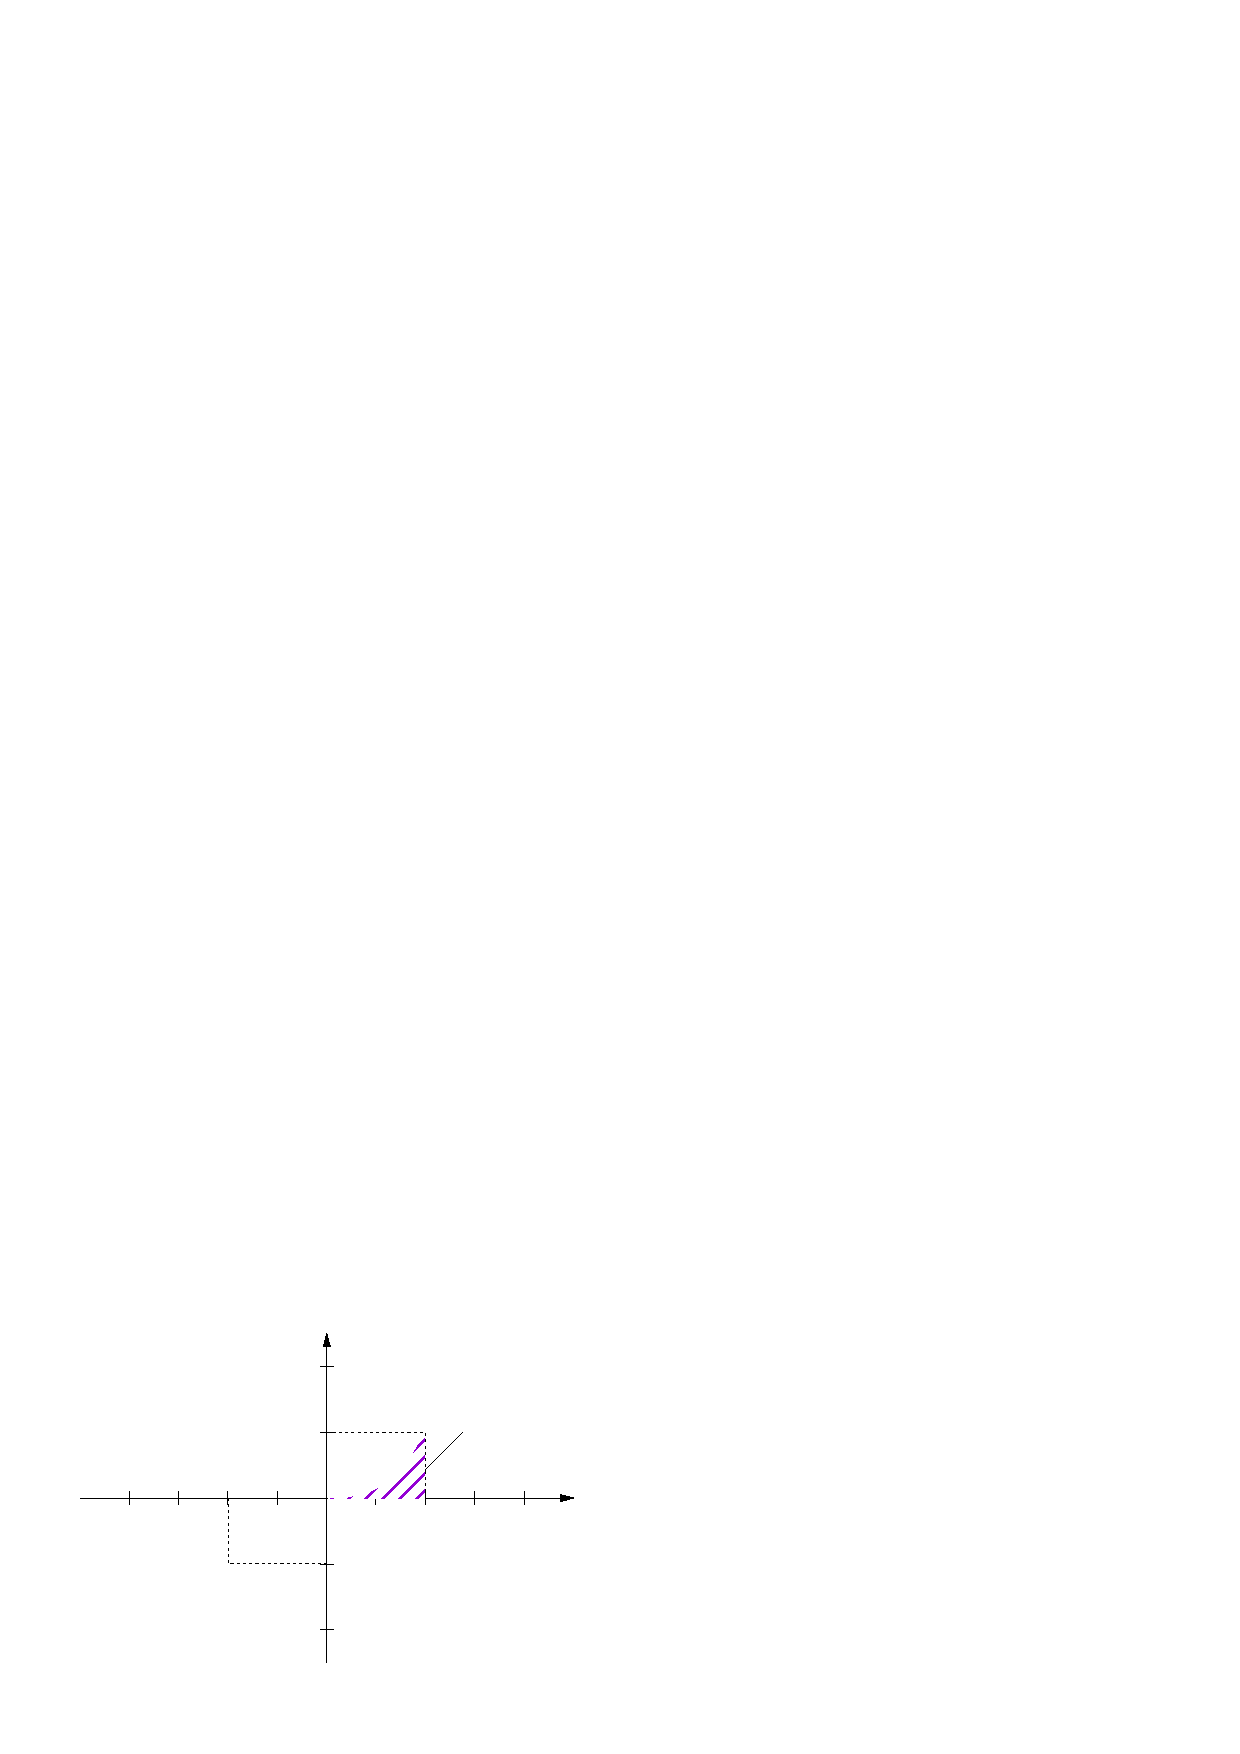
\includegraphics[width={216.00bp},height={144.00bp}]{figura_02_05}}%
    \gplfronttext
  \end{picture}%
\endgroup

\end{figure}

\underline{Prueba}:
\begin{equation*}
\begin{split}
    \int_{-a}^a\,f(t)\,dt
        &=\int_{-a}^0\,f(t)\,dt+\int_0^a\,f(t)\,dt\\
        &=\int_{-a}^0\,-f(-t)\,dt+\int_0^a\,f(t)\,dt\\
\end{split}
\end{equation*}
\begin{equation*}
    \tau=-t
\end{equation*}
\begin{equation*}
    d\tau=-dt
\end{equation*}
\begin{equation*}
\begin{split}
    \int_{-a}^a\,f(t)\,dt
        &=-\int_a^0\,f(\tau)\,(-d\tau)+\int_0^a\,f(t)\,dt\\
        &=-\int_0^a\,f(\tau)\,d\tau+\int_0^a\,f(t)\,dt\\
        &=0\\
\end{split}
\end{equation*}

\subsection{Evaluación de coeficientes de \emph{Fourier}}
\subsubsection{Simetría par}
\begin{equation*}
\begin{split}
    a_0
        &=\frac{2}{T}\int_0^T\,f(t)\,dt\\
        &=\frac{2}{T}\int_{-T/2}^{T/2}\,f(t)\,dt\\
        &=\frac{2}{T}\left(2\int_0^{T/2}\,f(t)\,dt\right)\\
        &=\frac{4}{T}\int_0^{T/2}\,f(t)\,dt\\
\end{split}
\end{equation*}
\begin{equation}
    a_0=\frac{4}{T}\int_0^{T/2}\,f(t)\,dt
\end{equation}
\begin{equation*}
\begin{split}
    a_n
        &=\frac{2}{T}\int_{-T/2}^{T/2}f(t)\cos(n\omega_0\,t)\,dt\\
        &=\frac{2}{T}\left(2\int_0^{T/2}f(t)\cos(n\omega_0\,t)\,dt\right)\\
        &=\frac{4}{T}\int_0^{T/2}f(t)\cos(n\omega_0\,t)\,dt\\
\end{split}
\end{equation*}
\begin{equation}
    a_n=\frac{4}{T}\int_0^{T/2}f(t)\cos(n\omega_0\,t)\,dt
\end{equation}
\begin{equation*}
\begin{split}
    b_n
        &=\frac{2}{T}\int_{-T/2}^{T/2}f(t)\sen(n\omega_0\,t)\,dt\\
        &=0\\
\end{split}
\end{equation*}
\begin{equation}
    b_n=0
\end{equation}

\subsubsection{Simetría impar}
\begin{equation*}
\begin{split}
    a_0
        &=\frac{2}{T}\int_0^T\,f(t)\,dt\\
        &=\frac{2}{T}\int_{-T/2}^{T/2}\,f(t)\,dt\\
        &=0\\
\end{split}
\end{equation*}
\begin{equation}
    a_0=0
\end{equation}
\begin{equation*}
\begin{split}
    a_n
        &=\frac{2}{T}\int_{-T/2}^{T/2}\,f(t)\cos(n\omega_0\,t)\,dt\\
        &=0\\
\end{split}
\end{equation*}
\begin{equation}
    a_n=0
\end{equation}
\begin{equation*}
\begin{split}
    b_n
        &=\frac{2}{T}\int_{-T/2}^{T/2}\,f(t)\sen(n\omega_0\,t)\,dt\\
        &=\frac{2}{T}\left(2\int_0^{T/2}\,f(t)\sen(n\omega_0\,t)\,dt\right)\\
        &=\frac{4}{T}\int_0^{T/2}f(t)\sen(n\omega_0\,t)\,dt\\
\end{split}
\end{equation*}
\begin{equation}
    b_n=\frac{4}{T}\int_0^{T/2}f(t)\sen(n\omega_0\,t)\,dt
\end{equation}

\section{Simetría de media onda (S.M.O.)}
$f(t)$ tiene simetría de media onda si:
\begin{equation*}
    f(t)=-f(t\pm\frac{T}{2})
\end{equation*}
\begin{figure}[H]
    \centering
    % GNUPLOT: LaTeX picture with Postscript
\begingroup
  \makeatletter
  \providecommand\color[2][]{%
    \GenericError{(gnuplot) \space\space\space\@spaces}{%
      Package color not loaded in conjunction with
      terminal option `colourtext'%
    }{See the gnuplot documentation for explanation.%
    }{Either use 'blacktext' in gnuplot or load the package
      color.sty in LaTeX.}%
    \renewcommand\color[2][]{}%
  }%
  \providecommand\includegraphics[2][]{%
    \GenericError{(gnuplot) \space\space\space\@spaces}{%
      Package graphicx or graphics not loaded%
    }{See the gnuplot documentation for explanation.%
    }{The gnuplot epslatex terminal needs graphicx.sty or graphics.sty.}%
    \renewcommand\includegraphics[2][]{}%
  }%
  \providecommand\rotatebox[2]{#2}%
  \@ifundefined{ifGPcolor}{%
    \newif\ifGPcolor
    \GPcolorfalse
  }{}%
  \@ifundefined{ifGPblacktext}{%
    \newif\ifGPblacktext
    \GPblacktexttrue
  }{}%
  % define a \g@addto@macro without @ in the name:
  \let\gplgaddtomacro\g@addto@macro
  % define empty templates for all commands taking text:
  \gdef\gplbacktext{}%
  \gdef\gplfronttext{}%
  \makeatother
  \ifGPblacktext
    % no textcolor at all
    \def\colorrgb#1{}%
    \def\colorgray#1{}%
  \else
    % gray or color?
    \ifGPcolor
      \def\colorrgb#1{\color[rgb]{#1}}%
      \def\colorgray#1{\color[gray]{#1}}%
      \expandafter\def\csname LTw\endcsname{\color{white}}%
      \expandafter\def\csname LTb\endcsname{\color{black}}%
      \expandafter\def\csname LTa\endcsname{\color{black}}%
      \expandafter\def\csname LT0\endcsname{\color[rgb]{1,0,0}}%
      \expandafter\def\csname LT1\endcsname{\color[rgb]{0,1,0}}%
      \expandafter\def\csname LT2\endcsname{\color[rgb]{0,0,1}}%
      \expandafter\def\csname LT3\endcsname{\color[rgb]{1,0,1}}%
      \expandafter\def\csname LT4\endcsname{\color[rgb]{0,1,1}}%
      \expandafter\def\csname LT5\endcsname{\color[rgb]{1,1,0}}%
      \expandafter\def\csname LT6\endcsname{\color[rgb]{0,0,0}}%
      \expandafter\def\csname LT7\endcsname{\color[rgb]{1,0.3,0}}%
      \expandafter\def\csname LT8\endcsname{\color[rgb]{0.5,0.5,0.5}}%
    \else
      % gray
      \def\colorrgb#1{\color{black}}%
      \def\colorgray#1{\color[gray]{#1}}%
      \expandafter\def\csname LTw\endcsname{\color{white}}%
      \expandafter\def\csname LTb\endcsname{\color{black}}%
      \expandafter\def\csname LTa\endcsname{\color{black}}%
      \expandafter\def\csname LT0\endcsname{\color{black}}%
      \expandafter\def\csname LT1\endcsname{\color{black}}%
      \expandafter\def\csname LT2\endcsname{\color{black}}%
      \expandafter\def\csname LT3\endcsname{\color{black}}%
      \expandafter\def\csname LT4\endcsname{\color{black}}%
      \expandafter\def\csname LT5\endcsname{\color{black}}%
      \expandafter\def\csname LT6\endcsname{\color{black}}%
      \expandafter\def\csname LT7\endcsname{\color{black}}%
      \expandafter\def\csname LT8\endcsname{\color{black}}%
    \fi
  \fi
    \setlength{\unitlength}{0.0500bp}%
    \ifx\gptboxheight\undefined%
      \newlength{\gptboxheight}%
      \newlength{\gptboxwidth}%
      \newsavebox{\gptboxtext}%
    \fi%
    \setlength{\fboxrule}{0.5pt}%
    \setlength{\fboxsep}{1pt}%
    \definecolor{tbcol}{rgb}{1,1,1}%
\begin{picture}(4320.00,3456.00)%
    \gplgaddtomacro\gplbacktext{%
      \csname LTb\endcsname%%
      \put(2040,192){\makebox(0,0)[r]{\strut{}}}%
      \put(2040,968){\makebox(0,0)[r]{\strut{}}}%
      \put(2040,1744){\makebox(0,0)[r]{\strut{}}}%
      \put(2040,2519){\makebox(0,0)[r]{\strut{}}}%
      \put(2040,3295){\makebox(0,0)[r]{\strut{}}}%
      \put(240,1521){\makebox(0,0){\strut{}}}%
      \put(714,1521){\makebox(0,0){\strut{}}}%
      \put(1188,1521){\makebox(0,0){\strut{}}}%
      \put(1662,1521){\makebox(0,0){\strut{}}}%
      \put(2136,1521){\makebox(0,0){\strut{}}}%
      \put(2609,1521){\makebox(0,0){\strut{}}}%
      \put(3083,1521){\makebox(0,0){\strut{}}}%
      \put(3557,1521){\makebox(0,0){\strut{}}}%
      \put(4031,1521){\makebox(0,0){\strut{}}}%
      \csname LTb\endcsname%%
      \put(4647,1744){\makebox(0,0)[l]{\strut{}$t$}}%
      \put(2349,3605){\makebox(0,0)[l]{\strut{}$f(t)$}}%
      \put(50,1511){\makebox(0,0)[l]{\strut{}$-T$}}%
      \put(998,1511){\makebox(0,0)[l]{\strut{}$-\frac{T}{2}$}}%
      \put(2988,1511){\makebox(0,0)[l]{\strut{}$ \frac{T}{2}$}}%
      \put(3984,1511){\makebox(0,0)[l]{\strut{}$T$}}%
    }%
    \gplgaddtomacro\gplfronttext{%
    }%
    \gplgaddtomacro\gplbacktext{%
      \csname LTb\endcsname%%
      \put(2040,192){\makebox(0,0)[r]{\strut{}}}%
      \put(2040,968){\makebox(0,0)[r]{\strut{}}}%
      \put(2040,1744){\makebox(0,0)[r]{\strut{}}}%
      \put(2040,2519){\makebox(0,0)[r]{\strut{}}}%
      \put(2040,3295){\makebox(0,0)[r]{\strut{}}}%
      \put(240,1521){\makebox(0,0){\strut{}}}%
      \put(714,1521){\makebox(0,0){\strut{}}}%
      \put(1188,1521){\makebox(0,0){\strut{}}}%
      \put(1662,1521){\makebox(0,0){\strut{}}}%
      \put(2136,1521){\makebox(0,0){\strut{}}}%
      \put(2609,1521){\makebox(0,0){\strut{}}}%
      \put(3083,1521){\makebox(0,0){\strut{}}}%
      \put(3557,1521){\makebox(0,0){\strut{}}}%
      \put(4031,1521){\makebox(0,0){\strut{}}}%
      \csname LTb\endcsname%%
      \put(4647,1744){\makebox(0,0)[l]{\strut{}$t$}}%
      \put(2349,3605){\makebox(0,0)[l]{\strut{}$f(t)$}}%
      \put(50,1511){\makebox(0,0)[l]{\strut{}$-T$}}%
      \put(998,1511){\makebox(0,0)[l]{\strut{}$-\frac{T}{2}$}}%
      \put(2988,1511){\makebox(0,0)[l]{\strut{}$ \frac{T}{2}$}}%
      \put(3984,1511){\makebox(0,0)[l]{\strut{}$T$}}%
    }%
    \gplgaddtomacro\gplfronttext{%
    }%
    \gplgaddtomacro\gplbacktext{%
      \csname LTb\endcsname%%
      \put(2040,192){\makebox(0,0)[r]{\strut{}}}%
      \put(2040,968){\makebox(0,0)[r]{\strut{}}}%
      \put(2040,1744){\makebox(0,0)[r]{\strut{}}}%
      \put(2040,2519){\makebox(0,0)[r]{\strut{}}}%
      \put(2040,3295){\makebox(0,0)[r]{\strut{}}}%
      \put(240,1521){\makebox(0,0){\strut{}}}%
      \put(714,1521){\makebox(0,0){\strut{}}}%
      \put(1188,1521){\makebox(0,0){\strut{}}}%
      \put(1662,1521){\makebox(0,0){\strut{}}}%
      \put(2136,1521){\makebox(0,0){\strut{}}}%
      \put(2609,1521){\makebox(0,0){\strut{}}}%
      \put(3083,1521){\makebox(0,0){\strut{}}}%
      \put(3557,1521){\makebox(0,0){\strut{}}}%
      \put(4031,1521){\makebox(0,0){\strut{}}}%
      \csname LTb\endcsname%%
      \put(4647,1744){\makebox(0,0)[l]{\strut{}$t$}}%
      \put(2349,3605){\makebox(0,0)[l]{\strut{}$f(t)$}}%
      \put(50,1511){\makebox(0,0)[l]{\strut{}$-T$}}%
      \put(998,1511){\makebox(0,0)[l]{\strut{}$-\frac{T}{2}$}}%
      \put(2988,1511){\makebox(0,0)[l]{\strut{}$ \frac{T}{2}$}}%
      \put(3984,1511){\makebox(0,0)[l]{\strut{}$T$}}%
    }%
    \gplgaddtomacro\gplfronttext{%
    }%
    \gplgaddtomacro\gplbacktext{%
      \csname LTb\endcsname%%
      \put(2040,192){\makebox(0,0)[r]{\strut{}}}%
      \put(2040,968){\makebox(0,0)[r]{\strut{}}}%
      \put(2040,1744){\makebox(0,0)[r]{\strut{}}}%
      \put(2040,2519){\makebox(0,0)[r]{\strut{}}}%
      \put(2040,3295){\makebox(0,0)[r]{\strut{}}}%
      \put(240,1521){\makebox(0,0){\strut{}}}%
      \put(714,1521){\makebox(0,0){\strut{}}}%
      \put(1188,1521){\makebox(0,0){\strut{}}}%
      \put(1662,1521){\makebox(0,0){\strut{}}}%
      \put(2136,1521){\makebox(0,0){\strut{}}}%
      \put(2609,1521){\makebox(0,0){\strut{}}}%
      \put(3083,1521){\makebox(0,0){\strut{}}}%
      \put(3557,1521){\makebox(0,0){\strut{}}}%
      \put(4031,1521){\makebox(0,0){\strut{}}}%
      \csname LTb\endcsname%%
      \put(4647,1744){\makebox(0,0)[l]{\strut{}$t$}}%
      \put(2349,3605){\makebox(0,0)[l]{\strut{}$f(t)$}}%
      \put(50,1511){\makebox(0,0)[l]{\strut{}$-T$}}%
      \put(998,1511){\makebox(0,0)[l]{\strut{}$-\frac{T}{2}$}}%
      \put(2988,1511){\makebox(0,0)[l]{\strut{}$ \frac{T}{2}$}}%
      \put(3984,1511){\makebox(0,0)[l]{\strut{}$T$}}%
    }%
    \gplgaddtomacro\gplfronttext{%
    }%
    \gplbacktext
    \put(0,0){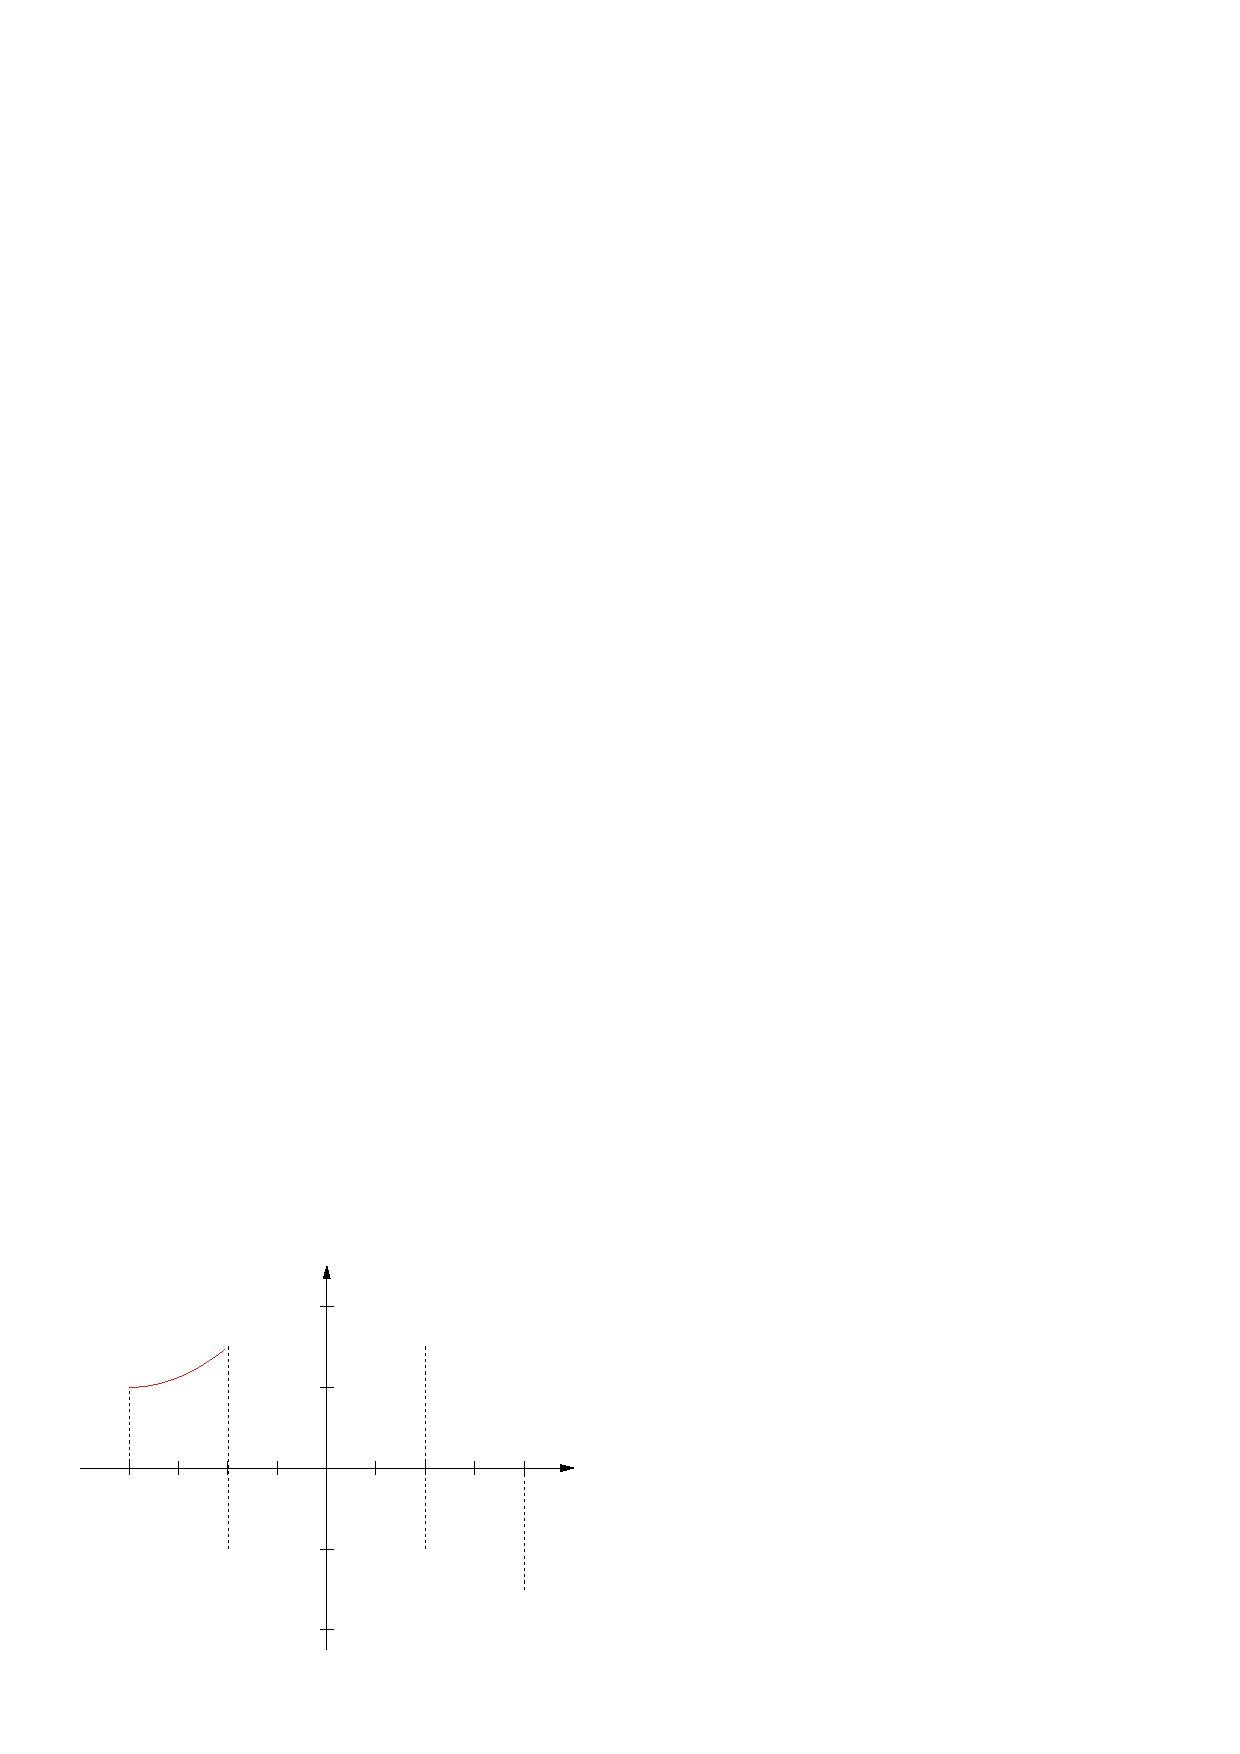
\includegraphics[width={216.00bp},height={172.80bp}]{figura_02_06}}%
    \gplfronttext
  \end{picture}%
\endgroup

    \caption{La gráfica se desplaza $1/2$ periodo\\
    y se refleja respecto a $t$.}
\end{figure}

\subsection{Evaluación de coeficientes de \emph{Fourier}}
\begin{equation*}
\begin{split}
    a_0
        &=\frac{2}{T}\int_0^T\,f(t)\,dt\\
        &=\frac{2}{T}\left[\int_0^{T/2}f(t)\,dt+\int_{T/2}^T\,f(t)\,dt\right]\\
        &=\frac{2}{T}\left[
            \int_0^{T/2}f(t)\,dt-\int_{t=T/2}^{t=T}f(t-\frac{T}{2})\,dt
        \right]\\
\end{split}
\end{equation*}
\begin{equation*}
    \tau=t-\frac{T}{2}
\end{equation*}
\begin{equation*}
    d\tau=dt
\end{equation*}
\begin{equation*}
\begin{split}
    a_0
        &=\frac{2}{T}\left[
            \int_0^{T/2}f(t)\,dt-
            \int_{\tau=T/2-T/2}^{\tau=T-T/2}f(\tau)\,d\tau
        \right]\\
        &=\frac{2}{T}\left[
            \int_0^{T/2}f(t)\,dt-\int_0^{T/2}f(\tau)\,d\tau
        \right]\\
\end{split}
\end{equation*}
\begin{equation}
    a_0=0
\end{equation}
\begin{equation*}
\begin{split}
    a_n
        &=\frac{2}{T}\int_0^T\,f(t)\cos(n\omega_0\,t)\,dt\\
        &=\frac{2}{T}\left[
            \int_0^{T/2}f(t)\cos(n\omega_0\,t)\,dt+
            \int_{T/2}^T\,f(t)\cos(n\omega_0\,t)\,dt
        \right]\\
        &=\frac{2}{T}\left[
            \int_0^{T/2}f(t)\cos(n\omega_0\,t)\,dt-
            \int_{T/2}^T\,f(t-\frac{T}{2})\cos(n\omega_0\,t)\,dt
        \right]\\
\end{split}
\end{equation*}
\begin{equation*}
    \tau=t-\frac{T}{2}
\end{equation*}
\begin{equation*}
    d\tau=dt
\end{equation*}
\begin{equation*}
\begin{split}
    a_n
        &=\frac{2}{T}\left[
            \int_0^{T/2}f(t)\cos(n\omega_0\,t)\,dt-
            \int_{\tau=T/2-T/2}^{\tau=T-T/2}
                f(\tau)\cos(n\omega_0(\tau+\frac{T}{2}))\,d\tau
        \right]\\
        &=\frac{2}{T}\left[
            \int_0^{T/2}f(t)\cos(n\omega_0\,t)\,dt-
            \int_0^{T/2}f(\tau)\cos(n\omega_0(\tau+\frac{T}{2}))\,d\tau
        \right]\\
\end{split}
\end{equation*}
\begin{equation*}
\begin{split}
    n\omega_0(\tau+T/2)
        &=n\omega_0\tau+n\omega_0\frac{T}{2}\\
        &=n\omega_0\tau+n\frac{2\pi}{T}\frac{T}{2}\\
        &=n\omega_0\tau+n\pi\\
\end{split}
\end{equation*}
\begin{equation*}
\begin{split}
    \cos(n\omega_0\tau+n\pi)
        &=\cos(n\omega_0\tau)\cos(n\pi)-\sen(n\pi)\sen(n\omega_0\tau)\\
        &=\cos(n\omega_0\tau)\cos(n\pi)\\
\end{split}
\end{equation*}
\begin{equation*}
\begin{split}
    a_n
        &=\frac{2}{T}\left[
            \int_0^{T/2}f(t)\cos(n\omega_0\,t)\,dt-
            \int_0^{T/2}f(\tau)\cos(n\omega_0\tau)\cos(n\pi)\,d\tau
        \right]\\
        &=\frac{2}{T}\left[
            \int_0^{T/2}f(t)\cos(n\omega_0\,t)\,dt-\cos(n\pi)\int_0^{T/2}
                f(\tau)\cos(n\omega_0\tau)\,d\tau
        \right]\\
        &=\frac{2}{T}(1-\cos(\pi\,n))\left(
            \int_0^{T/2}f(t)\cos(n\omega_0\,t)\,dt
        \right)\\
\end{split}
\end{equation*}
\begin{equation*}
    \cos(\pi\,n)=\begin{cases}
        1&n:\text{par}\\
        -1&n:\text{impar}\\
    \end{cases}
\end{equation*}
\begin{equation}
\begin{cases}
    n:\text{par}&a_n=0\\
    n:\text{impar}&a_n=\frac{4}{T}\int_0^{T/2}f(t)\cos(n\omega_0\,t)\,dt\\
\end{cases}
\end{equation}
\begin{equation*}
\begin{split}
    b_n
        &=\frac{2}{T}\int_0^T\,f(t)\sen(n\omega_0\,t)\,dt\\
        &=\frac{2}{T}\left[
            \int_0^{T/2}\,f(t)\sen(n\omega_0\,t)\,dt+
            \int_{T/2}^T\,f(t)\sen(n\omega_0\,t)\,dt
        \right]\\
        &=\frac{2}{T}\left[
            \int_0^{T/2}\,f(t)\sen(n\omega_0\,t)\,dt-
            \int_{T/2}^T\,f(t-\frac{T}{2})\sen(n\omega_0\,t)\,dt
        \right]\\
\end{split}
\end{equation*}
\begin{equation*}
    \tau=t-\frac{T}{2}
\end{equation*}
\begin{equation*}
    d\tau=dt
\end{equation*}
\begin{equation*}
\begin{split}
    b_n
        &=\frac{2}{T}\left[
            \int_0^{T/2}\,f(t)\sen(n\omega_0\,t)\,dt-
            \int_{\tau=T/2-T/2}^{\tau=T-T/2}
                f(\tau)\sen(n\omega_0(\tau+\frac{T}{2}))\,d\tau
        \right]\\
        &=\frac{2}{T}\left[
            \int_0^{T/2}\,f(t)\sen(n\omega_0\,t)\,dt-
            \int_0^{T/2}\,f(\tau)\sen(n\omega_0(\tau+\frac{T}{2}))\,d\tau
        \right]\\
\end{split}
\end{equation*}
\begin{equation*}
\begin{split}
    n\omega_0(\tau+T/2)
        &=n\omega_0\tau+n\omega_0\frac{T}{2}\\
        &=n\omega_0\tau+n\frac{2\pi}{T}\frac{T}{2}\\
        &=n\omega_0\tau+n\pi\\
\end{split}
\end{equation*}
\begin{equation*}
\begin{split}
    \sen(n\omega_0\tau+n\pi)
        &=\sen(n\omega_0\tau)\cos(n\pi)+\sen(n\pi)\cos(n\omega_0\tau)\\
        &=\sen(n\omega_0\tau)\cos(n\pi)\\
\end{split}
\end{equation*}
\begin{equation*}
\begin{split}
    b_n
        &=\frac{2}{T}\left[
            \int_0^{T/2}\,f(t)\sen(n\omega_0\,t)\,dt-
            \int_0^{T/2}\,f(\tau)\sen(n\omega_0\tau)\cos(n\pi)\,d\tau
        \right]\\
        &=\frac{2}{T}\left[
            \int_0^{T/2}\,f(t)\sen(n\omega_0\,t)\,dt-
            \cos(n\pi)\int_0^{T/2}\,f(\tau)\sen(n\omega_0\tau)\,d\tau
        \right]\\
        &=\frac{2}{T}(1-\cos(\pi\,n))\left(
            \int_0^{T/2}\,f(t)\sen(n\omega_0\,t)\,dt
        \right)\\
\end{split}
\end{equation*}
\begin{equation*}
    \cos(\pi\,n)=\begin{cases}
        1&n:\text{par}\\
        -1&n:\text{impar}\\
    \end{cases}
\end{equation*}
\begin{equation}
\begin{cases}
    n:\text{par}&b_n=0\\
    n:\text{impar}&b_n=\frac{4}{T}\int_0^{T/2}f(t)\sen(n\omega_0\,t)\,dt\\
\end{cases}
\end{equation}

\section{Simetría de cuarto de onda (S.C.O.)}
\subsection{Simetría de cuarto de onda par}
Una función $f(t)$ tiene simetría de cuarto de onda \textbf{par} cuando:
\begin{itemize}
    \item $f(t)$ es \textbf{par}.
    \item $f(t)$ tiene simetría de media onda.
\end{itemize}
\begin{figure}[H]
    \centering
    % GNUPLOT: LaTeX picture with Postscript
\begingroup
  \makeatletter
  \providecommand\color[2][]{%
    \GenericError{(gnuplot) \space\space\space\@spaces}{%
      Package color not loaded in conjunction with
      terminal option `colourtext'%
    }{See the gnuplot documentation for explanation.%
    }{Either use 'blacktext' in gnuplot or load the package
      color.sty in LaTeX.}%
    \renewcommand\color[2][]{}%
  }%
  \providecommand\includegraphics[2][]{%
    \GenericError{(gnuplot) \space\space\space\@spaces}{%
      Package graphicx or graphics not loaded%
    }{See the gnuplot documentation for explanation.%
    }{The gnuplot epslatex terminal needs graphicx.sty or graphics.sty.}%
    \renewcommand\includegraphics[2][]{}%
  }%
  \providecommand\rotatebox[2]{#2}%
  \@ifundefined{ifGPcolor}{%
    \newif\ifGPcolor
    \GPcolorfalse
  }{}%
  \@ifundefined{ifGPblacktext}{%
    \newif\ifGPblacktext
    \GPblacktexttrue
  }{}%
  % define a \g@addto@macro without @ in the name:
  \let\gplgaddtomacro\g@addto@macro
  % define empty templates for all commands taking text:
  \gdef\gplbacktext{}%
  \gdef\gplfronttext{}%
  \makeatother
  \ifGPblacktext
    % no textcolor at all
    \def\colorrgb#1{}%
    \def\colorgray#1{}%
  \else
    % gray or color?
    \ifGPcolor
      \def\colorrgb#1{\color[rgb]{#1}}%
      \def\colorgray#1{\color[gray]{#1}}%
      \expandafter\def\csname LTw\endcsname{\color{white}}%
      \expandafter\def\csname LTb\endcsname{\color{black}}%
      \expandafter\def\csname LTa\endcsname{\color{black}}%
      \expandafter\def\csname LT0\endcsname{\color[rgb]{1,0,0}}%
      \expandafter\def\csname LT1\endcsname{\color[rgb]{0,1,0}}%
      \expandafter\def\csname LT2\endcsname{\color[rgb]{0,0,1}}%
      \expandafter\def\csname LT3\endcsname{\color[rgb]{1,0,1}}%
      \expandafter\def\csname LT4\endcsname{\color[rgb]{0,1,1}}%
      \expandafter\def\csname LT5\endcsname{\color[rgb]{1,1,0}}%
      \expandafter\def\csname LT6\endcsname{\color[rgb]{0,0,0}}%
      \expandafter\def\csname LT7\endcsname{\color[rgb]{1,0.3,0}}%
      \expandafter\def\csname LT8\endcsname{\color[rgb]{0.5,0.5,0.5}}%
    \else
      % gray
      \def\colorrgb#1{\color{black}}%
      \def\colorgray#1{\color[gray]{#1}}%
      \expandafter\def\csname LTw\endcsname{\color{white}}%
      \expandafter\def\csname LTb\endcsname{\color{black}}%
      \expandafter\def\csname LTa\endcsname{\color{black}}%
      \expandafter\def\csname LT0\endcsname{\color{black}}%
      \expandafter\def\csname LT1\endcsname{\color{black}}%
      \expandafter\def\csname LT2\endcsname{\color{black}}%
      \expandafter\def\csname LT3\endcsname{\color{black}}%
      \expandafter\def\csname LT4\endcsname{\color{black}}%
      \expandafter\def\csname LT5\endcsname{\color{black}}%
      \expandafter\def\csname LT6\endcsname{\color{black}}%
      \expandafter\def\csname LT7\endcsname{\color{black}}%
      \expandafter\def\csname LT8\endcsname{\color{black}}%
    \fi
  \fi
    \setlength{\unitlength}{0.0500bp}%
    \ifx\gptboxheight\undefined%
      \newlength{\gptboxheight}%
      \newlength{\gptboxwidth}%
      \newsavebox{\gptboxtext}%
    \fi%
    \setlength{\fboxrule}{0.5pt}%
    \setlength{\fboxsep}{1pt}%
    \definecolor{tbcol}{rgb}{1,1,1}%
\begin{picture}(7200.00,3456.00)%
    \gplgaddtomacro\gplbacktext{%
      \csname LTb\endcsname%%
      \put(3480,192){\makebox(0,0)[r]{\strut{}}}%
      \put(3480,709){\makebox(0,0)[r]{\strut{}}}%
      \put(3480,1226){\makebox(0,0)[r]{\strut{}}}%
      \put(3480,1744){\makebox(0,0)[r]{\strut{}}}%
      \put(3480,2261){\makebox(0,0)[r]{\strut{}}}%
      \put(3480,2778){\makebox(0,0)[r]{\strut{}}}%
      \put(3480,3295){\makebox(0,0)[r]{\strut{}}}%
      \put(240,1521){\makebox(0,0){\strut{}}}%
      \put(907,1521){\makebox(0,0){\strut{}}}%
      \put(1574,1521){\makebox(0,0){\strut{}}}%
      \put(2241,1521){\makebox(0,0){\strut{}}}%
      \put(2908,1521){\makebox(0,0){\strut{}}}%
      \put(3576,1521){\makebox(0,0){\strut{}}}%
      \put(4243,1521){\makebox(0,0){\strut{}}}%
      \put(4910,1521){\makebox(0,0){\strut{}}}%
      \put(5577,1521){\makebox(0,0){\strut{}}}%
      \put(6244,1521){\makebox(0,0){\strut{}}}%
      \put(6911,1521){\makebox(0,0){\strut{}}}%
      \csname LTb\endcsname%%
      \put(7778,1744){\makebox(0,0)[l]{\strut{}$t$}}%
      \put(3876,3502){\makebox(0,0)[l]{\strut{}$f(t)$}}%
      \put(640,1485){\makebox(0,0)[l]{\strut{}$-T$}}%
      \put(1307,1485){\makebox(0,0)[l]{\strut{}$-\frac{3T}{4}$}}%
      \put(1974,1485){\makebox(0,0)[l]{\strut{}$-\frac{T}{2}$}}%
      \put(2642,1485){\makebox(0,0)[l]{\strut{}$-\frac{T}{4}$}}%
      \put(4176,1485){\makebox(0,0)[l]{\strut{}$ \frac{T}{4}$}}%
      \put(4776,1485){\makebox(0,0)[l]{\strut{}$ \frac{T}{2}$}}%
      \put(5443,1485){\makebox(0,0)[l]{\strut{}$ \frac{3T}{4}$}}%
      \put(6177,1485){\makebox(0,0)[l]{\strut{}$T$}}%
    }%
    \gplgaddtomacro\gplfronttext{%
    }%
    \gplgaddtomacro\gplbacktext{%
      \csname LTb\endcsname%%
      \put(3480,192){\makebox(0,0)[r]{\strut{}}}%
      \put(3480,709){\makebox(0,0)[r]{\strut{}}}%
      \put(3480,1226){\makebox(0,0)[r]{\strut{}}}%
      \put(3480,1744){\makebox(0,0)[r]{\strut{}}}%
      \put(3480,2261){\makebox(0,0)[r]{\strut{}}}%
      \put(3480,2778){\makebox(0,0)[r]{\strut{}}}%
      \put(3480,3295){\makebox(0,0)[r]{\strut{}}}%
      \put(240,1521){\makebox(0,0){\strut{}}}%
      \put(907,1521){\makebox(0,0){\strut{}}}%
      \put(1574,1521){\makebox(0,0){\strut{}}}%
      \put(2241,1521){\makebox(0,0){\strut{}}}%
      \put(2908,1521){\makebox(0,0){\strut{}}}%
      \put(3576,1521){\makebox(0,0){\strut{}}}%
      \put(4243,1521){\makebox(0,0){\strut{}}}%
      \put(4910,1521){\makebox(0,0){\strut{}}}%
      \put(5577,1521){\makebox(0,0){\strut{}}}%
      \put(6244,1521){\makebox(0,0){\strut{}}}%
      \put(6911,1521){\makebox(0,0){\strut{}}}%
      \csname LTb\endcsname%%
      \put(7778,1744){\makebox(0,0)[l]{\strut{}$t$}}%
      \put(3876,3502){\makebox(0,0)[l]{\strut{}$f(t)$}}%
      \put(640,1485){\makebox(0,0)[l]{\strut{}$-T$}}%
      \put(1307,1485){\makebox(0,0)[l]{\strut{}$-\frac{3T}{4}$}}%
      \put(1974,1485){\makebox(0,0)[l]{\strut{}$-\frac{T}{2}$}}%
      \put(2642,1485){\makebox(0,0)[l]{\strut{}$-\frac{T}{4}$}}%
      \put(4176,1485){\makebox(0,0)[l]{\strut{}$ \frac{T}{4}$}}%
      \put(4776,1485){\makebox(0,0)[l]{\strut{}$ \frac{T}{2}$}}%
      \put(5443,1485){\makebox(0,0)[l]{\strut{}$ \frac{3T}{4}$}}%
      \put(6177,1485){\makebox(0,0)[l]{\strut{}$T$}}%
    }%
    \gplgaddtomacro\gplfronttext{%
    }%
    \gplgaddtomacro\gplbacktext{%
      \csname LTb\endcsname%%
      \put(3480,192){\makebox(0,0)[r]{\strut{}}}%
      \put(3480,709){\makebox(0,0)[r]{\strut{}}}%
      \put(3480,1226){\makebox(0,0)[r]{\strut{}}}%
      \put(3480,1744){\makebox(0,0)[r]{\strut{}}}%
      \put(3480,2261){\makebox(0,0)[r]{\strut{}}}%
      \put(3480,2778){\makebox(0,0)[r]{\strut{}}}%
      \put(3480,3295){\makebox(0,0)[r]{\strut{}}}%
      \put(240,1521){\makebox(0,0){\strut{}}}%
      \put(907,1521){\makebox(0,0){\strut{}}}%
      \put(1574,1521){\makebox(0,0){\strut{}}}%
      \put(2241,1521){\makebox(0,0){\strut{}}}%
      \put(2908,1521){\makebox(0,0){\strut{}}}%
      \put(3576,1521){\makebox(0,0){\strut{}}}%
      \put(4243,1521){\makebox(0,0){\strut{}}}%
      \put(4910,1521){\makebox(0,0){\strut{}}}%
      \put(5577,1521){\makebox(0,0){\strut{}}}%
      \put(6244,1521){\makebox(0,0){\strut{}}}%
      \put(6911,1521){\makebox(0,0){\strut{}}}%
      \csname LTb\endcsname%%
      \put(7778,1744){\makebox(0,0)[l]{\strut{}$t$}}%
      \put(3876,3502){\makebox(0,0)[l]{\strut{}$f(t)$}}%
      \put(640,1485){\makebox(0,0)[l]{\strut{}$-T$}}%
      \put(1307,1485){\makebox(0,0)[l]{\strut{}$-\frac{3T}{4}$}}%
      \put(1974,1485){\makebox(0,0)[l]{\strut{}$-\frac{T}{2}$}}%
      \put(2642,1485){\makebox(0,0)[l]{\strut{}$-\frac{T}{4}$}}%
      \put(4176,1485){\makebox(0,0)[l]{\strut{}$ \frac{T}{4}$}}%
      \put(4776,1485){\makebox(0,0)[l]{\strut{}$ \frac{T}{2}$}}%
      \put(5443,1485){\makebox(0,0)[l]{\strut{}$ \frac{3T}{4}$}}%
      \put(6177,1485){\makebox(0,0)[l]{\strut{}$T$}}%
    }%
    \gplgaddtomacro\gplfronttext{%
    }%
    \gplgaddtomacro\gplbacktext{%
      \csname LTb\endcsname%%
      \put(3480,192){\makebox(0,0)[r]{\strut{}}}%
      \put(3480,709){\makebox(0,0)[r]{\strut{}}}%
      \put(3480,1226){\makebox(0,0)[r]{\strut{}}}%
      \put(3480,1744){\makebox(0,0)[r]{\strut{}}}%
      \put(3480,2261){\makebox(0,0)[r]{\strut{}}}%
      \put(3480,2778){\makebox(0,0)[r]{\strut{}}}%
      \put(3480,3295){\makebox(0,0)[r]{\strut{}}}%
      \put(240,1521){\makebox(0,0){\strut{}}}%
      \put(907,1521){\makebox(0,0){\strut{}}}%
      \put(1574,1521){\makebox(0,0){\strut{}}}%
      \put(2241,1521){\makebox(0,0){\strut{}}}%
      \put(2908,1521){\makebox(0,0){\strut{}}}%
      \put(3576,1521){\makebox(0,0){\strut{}}}%
      \put(4243,1521){\makebox(0,0){\strut{}}}%
      \put(4910,1521){\makebox(0,0){\strut{}}}%
      \put(5577,1521){\makebox(0,0){\strut{}}}%
      \put(6244,1521){\makebox(0,0){\strut{}}}%
      \put(6911,1521){\makebox(0,0){\strut{}}}%
      \csname LTb\endcsname%%
      \put(7778,1744){\makebox(0,0)[l]{\strut{}$t$}}%
      \put(3876,3502){\makebox(0,0)[l]{\strut{}$f(t)$}}%
      \put(640,1485){\makebox(0,0)[l]{\strut{}$-T$}}%
      \put(1307,1485){\makebox(0,0)[l]{\strut{}$-\frac{3T}{4}$}}%
      \put(1974,1485){\makebox(0,0)[l]{\strut{}$-\frac{T}{2}$}}%
      \put(2642,1485){\makebox(0,0)[l]{\strut{}$-\frac{T}{4}$}}%
      \put(4176,1485){\makebox(0,0)[l]{\strut{}$ \frac{T}{4}$}}%
      \put(4776,1485){\makebox(0,0)[l]{\strut{}$ \frac{T}{2}$}}%
      \put(5443,1485){\makebox(0,0)[l]{\strut{}$ \frac{3T}{4}$}}%
      \put(6177,1485){\makebox(0,0)[l]{\strut{}$T$}}%
    }%
    \gplgaddtomacro\gplfronttext{%
    }%
    \gplgaddtomacro\gplbacktext{%
      \csname LTb\endcsname%%
      \put(3480,192){\makebox(0,0)[r]{\strut{}}}%
      \put(3480,709){\makebox(0,0)[r]{\strut{}}}%
      \put(3480,1226){\makebox(0,0)[r]{\strut{}}}%
      \put(3480,1744){\makebox(0,0)[r]{\strut{}}}%
      \put(3480,2261){\makebox(0,0)[r]{\strut{}}}%
      \put(3480,2778){\makebox(0,0)[r]{\strut{}}}%
      \put(3480,3295){\makebox(0,0)[r]{\strut{}}}%
      \put(240,1521){\makebox(0,0){\strut{}}}%
      \put(907,1521){\makebox(0,0){\strut{}}}%
      \put(1574,1521){\makebox(0,0){\strut{}}}%
      \put(2241,1521){\makebox(0,0){\strut{}}}%
      \put(2908,1521){\makebox(0,0){\strut{}}}%
      \put(3576,1521){\makebox(0,0){\strut{}}}%
      \put(4243,1521){\makebox(0,0){\strut{}}}%
      \put(4910,1521){\makebox(0,0){\strut{}}}%
      \put(5577,1521){\makebox(0,0){\strut{}}}%
      \put(6244,1521){\makebox(0,0){\strut{}}}%
      \put(6911,1521){\makebox(0,0){\strut{}}}%
      \csname LTb\endcsname%%
      \put(7778,1744){\makebox(0,0)[l]{\strut{}$t$}}%
      \put(3876,3502){\makebox(0,0)[l]{\strut{}$f(t)$}}%
      \put(640,1485){\makebox(0,0)[l]{\strut{}$-T$}}%
      \put(1307,1485){\makebox(0,0)[l]{\strut{}$-\frac{3T}{4}$}}%
      \put(1974,1485){\makebox(0,0)[l]{\strut{}$-\frac{T}{2}$}}%
      \put(2642,1485){\makebox(0,0)[l]{\strut{}$-\frac{T}{4}$}}%
      \put(4176,1485){\makebox(0,0)[l]{\strut{}$ \frac{T}{4}$}}%
      \put(4776,1485){\makebox(0,0)[l]{\strut{}$ \frac{T}{2}$}}%
      \put(5443,1485){\makebox(0,0)[l]{\strut{}$ \frac{3T}{4}$}}%
      \put(6177,1485){\makebox(0,0)[l]{\strut{}$T$}}%
    }%
    \gplgaddtomacro\gplfronttext{%
    }%
    \gplbacktext
    \put(0,0){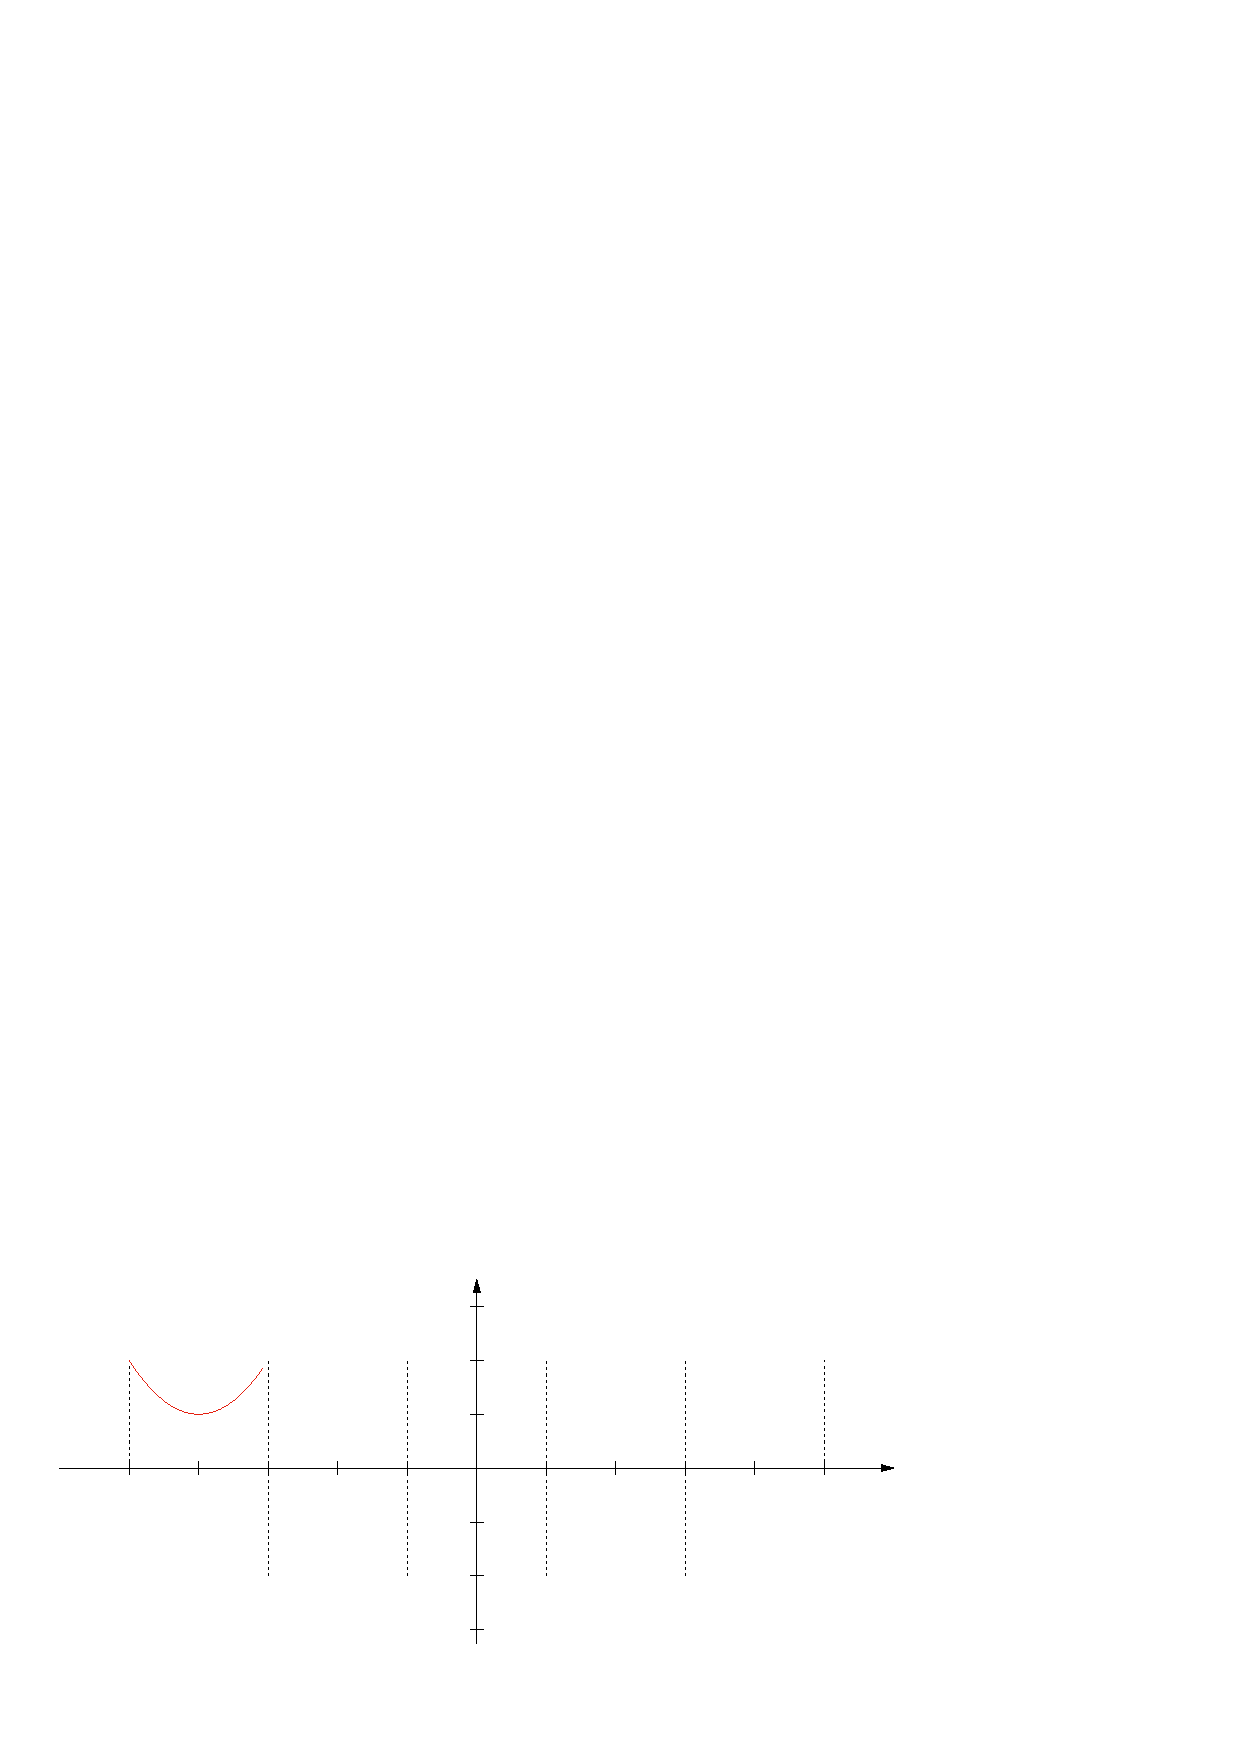
\includegraphics[width={360.00bp},height={172.80bp}]{figura_02_07}}%
    \gplfronttext
  \end{picture}%
\endgroup

\end{figure}

\subsection{Simetría de cuarto de onda impar}
Una función $f(t)$ tiene simetría de cuarto de onda \textbf{impar} cuando:
\begin{itemize}
    \item $f(t)$ es \textbf{impar}.
    \item $f(t)$ tiene simetría de media onda.
\end{itemize}
\begin{figure}[H]
    \centering
    % GNUPLOT: LaTeX picture with Postscript
\begingroup
  \makeatletter
  \providecommand\color[2][]{%
    \GenericError{(gnuplot) \space\space\space\@spaces}{%
      Package color not loaded in conjunction with
      terminal option `colourtext'%
    }{See the gnuplot documentation for explanation.%
    }{Either use 'blacktext' in gnuplot or load the package
      color.sty in LaTeX.}%
    \renewcommand\color[2][]{}%
  }%
  \providecommand\includegraphics[2][]{%
    \GenericError{(gnuplot) \space\space\space\@spaces}{%
      Package graphicx or graphics not loaded%
    }{See the gnuplot documentation for explanation.%
    }{The gnuplot epslatex terminal needs graphicx.sty or graphics.sty.}%
    \renewcommand\includegraphics[2][]{}%
  }%
  \providecommand\rotatebox[2]{#2}%
  \@ifundefined{ifGPcolor}{%
    \newif\ifGPcolor
    \GPcolorfalse
  }{}%
  \@ifundefined{ifGPblacktext}{%
    \newif\ifGPblacktext
    \GPblacktexttrue
  }{}%
  % define a \g@addto@macro without @ in the name:
  \let\gplgaddtomacro\g@addto@macro
  % define empty templates for all commands taking text:
  \gdef\gplbacktext{}%
  \gdef\gplfronttext{}%
  \makeatother
  \ifGPblacktext
    % no textcolor at all
    \def\colorrgb#1{}%
    \def\colorgray#1{}%
  \else
    % gray or color?
    \ifGPcolor
      \def\colorrgb#1{\color[rgb]{#1}}%
      \def\colorgray#1{\color[gray]{#1}}%
      \expandafter\def\csname LTw\endcsname{\color{white}}%
      \expandafter\def\csname LTb\endcsname{\color{black}}%
      \expandafter\def\csname LTa\endcsname{\color{black}}%
      \expandafter\def\csname LT0\endcsname{\color[rgb]{1,0,0}}%
      \expandafter\def\csname LT1\endcsname{\color[rgb]{0,1,0}}%
      \expandafter\def\csname LT2\endcsname{\color[rgb]{0,0,1}}%
      \expandafter\def\csname LT3\endcsname{\color[rgb]{1,0,1}}%
      \expandafter\def\csname LT4\endcsname{\color[rgb]{0,1,1}}%
      \expandafter\def\csname LT5\endcsname{\color[rgb]{1,1,0}}%
      \expandafter\def\csname LT6\endcsname{\color[rgb]{0,0,0}}%
      \expandafter\def\csname LT7\endcsname{\color[rgb]{1,0.3,0}}%
      \expandafter\def\csname LT8\endcsname{\color[rgb]{0.5,0.5,0.5}}%
    \else
      % gray
      \def\colorrgb#1{\color{black}}%
      \def\colorgray#1{\color[gray]{#1}}%
      \expandafter\def\csname LTw\endcsname{\color{white}}%
      \expandafter\def\csname LTb\endcsname{\color{black}}%
      \expandafter\def\csname LTa\endcsname{\color{black}}%
      \expandafter\def\csname LT0\endcsname{\color{black}}%
      \expandafter\def\csname LT1\endcsname{\color{black}}%
      \expandafter\def\csname LT2\endcsname{\color{black}}%
      \expandafter\def\csname LT3\endcsname{\color{black}}%
      \expandafter\def\csname LT4\endcsname{\color{black}}%
      \expandafter\def\csname LT5\endcsname{\color{black}}%
      \expandafter\def\csname LT6\endcsname{\color{black}}%
      \expandafter\def\csname LT7\endcsname{\color{black}}%
      \expandafter\def\csname LT8\endcsname{\color{black}}%
    \fi
  \fi
    \setlength{\unitlength}{0.0500bp}%
    \ifx\gptboxheight\undefined%
      \newlength{\gptboxheight}%
      \newlength{\gptboxwidth}%
      \newsavebox{\gptboxtext}%
    \fi%
    \setlength{\fboxrule}{0.5pt}%
    \setlength{\fboxsep}{1pt}%
    \definecolor{tbcol}{rgb}{1,1,1}%
\begin{picture}(7200.00,3456.00)%
    \gplgaddtomacro\gplbacktext{%
      \csname LTb\endcsname%%
      \put(3480,192){\makebox(0,0)[r]{\strut{}}}%
      \put(3480,709){\makebox(0,0)[r]{\strut{}}}%
      \put(3480,1226){\makebox(0,0)[r]{\strut{}}}%
      \put(3480,1744){\makebox(0,0)[r]{\strut{}}}%
      \put(3480,2261){\makebox(0,0)[r]{\strut{}}}%
      \put(3480,2778){\makebox(0,0)[r]{\strut{}}}%
      \put(3480,3295){\makebox(0,0)[r]{\strut{}}}%
      \put(240,1521){\makebox(0,0){\strut{}}}%
      \put(907,1521){\makebox(0,0){\strut{}}}%
      \put(1574,1521){\makebox(0,0){\strut{}}}%
      \put(2241,1521){\makebox(0,0){\strut{}}}%
      \put(2908,1521){\makebox(0,0){\strut{}}}%
      \put(3576,1521){\makebox(0,0){\strut{}}}%
      \put(4243,1521){\makebox(0,0){\strut{}}}%
      \put(4910,1521){\makebox(0,0){\strut{}}}%
      \put(5577,1521){\makebox(0,0){\strut{}}}%
      \put(6244,1521){\makebox(0,0){\strut{}}}%
      \put(6911,1521){\makebox(0,0){\strut{}}}%
      \csname LTb\endcsname%%
      \put(7778,1744){\makebox(0,0)[l]{\strut{}$t$}}%
      \put(3876,3502){\makebox(0,0)[l]{\strut{}$f(t)$}}%
      \put(640,1485){\makebox(0,0)[l]{\strut{}$-T$}}%
      \put(1307,1485){\makebox(0,0)[l]{\strut{}$-\frac{3T}{4}$}}%
      \put(1974,1485){\makebox(0,0)[l]{\strut{}$-\frac{T}{2}$}}%
      \put(2642,1485){\makebox(0,0)[l]{\strut{}$-\frac{T}{4}$}}%
      \put(4176,1485){\makebox(0,0)[l]{\strut{}$ \frac{T}{4}$}}%
      \put(4776,1485){\makebox(0,0)[l]{\strut{}$ \frac{T}{2}$}}%
      \put(5443,1485){\makebox(0,0)[l]{\strut{}$ \frac{3T}{4}$}}%
      \put(6177,1485){\makebox(0,0)[l]{\strut{}$T$}}%
    }%
    \gplgaddtomacro\gplfronttext{%
    }%
    \gplgaddtomacro\gplbacktext{%
      \csname LTb\endcsname%%
      \put(3480,192){\makebox(0,0)[r]{\strut{}}}%
      \put(3480,709){\makebox(0,0)[r]{\strut{}}}%
      \put(3480,1226){\makebox(0,0)[r]{\strut{}}}%
      \put(3480,1744){\makebox(0,0)[r]{\strut{}}}%
      \put(3480,2261){\makebox(0,0)[r]{\strut{}}}%
      \put(3480,2778){\makebox(0,0)[r]{\strut{}}}%
      \put(3480,3295){\makebox(0,0)[r]{\strut{}}}%
      \put(240,1521){\makebox(0,0){\strut{}}}%
      \put(907,1521){\makebox(0,0){\strut{}}}%
      \put(1574,1521){\makebox(0,0){\strut{}}}%
      \put(2241,1521){\makebox(0,0){\strut{}}}%
      \put(2908,1521){\makebox(0,0){\strut{}}}%
      \put(3576,1521){\makebox(0,0){\strut{}}}%
      \put(4243,1521){\makebox(0,0){\strut{}}}%
      \put(4910,1521){\makebox(0,0){\strut{}}}%
      \put(5577,1521){\makebox(0,0){\strut{}}}%
      \put(6244,1521){\makebox(0,0){\strut{}}}%
      \put(6911,1521){\makebox(0,0){\strut{}}}%
      \csname LTb\endcsname%%
      \put(7778,1744){\makebox(0,0)[l]{\strut{}$t$}}%
      \put(3876,3502){\makebox(0,0)[l]{\strut{}$f(t)$}}%
      \put(640,1485){\makebox(0,0)[l]{\strut{}$-T$}}%
      \put(1307,1485){\makebox(0,0)[l]{\strut{}$-\frac{3T}{4}$}}%
      \put(1974,1485){\makebox(0,0)[l]{\strut{}$-\frac{T}{2}$}}%
      \put(2642,1485){\makebox(0,0)[l]{\strut{}$-\frac{T}{4}$}}%
      \put(4176,1485){\makebox(0,0)[l]{\strut{}$ \frac{T}{4}$}}%
      \put(4776,1485){\makebox(0,0)[l]{\strut{}$ \frac{T}{2}$}}%
      \put(5443,1485){\makebox(0,0)[l]{\strut{}$ \frac{3T}{4}$}}%
      \put(6177,1485){\makebox(0,0)[l]{\strut{}$T$}}%
    }%
    \gplgaddtomacro\gplfronttext{%
    }%
    \gplgaddtomacro\gplbacktext{%
      \csname LTb\endcsname%%
      \put(3480,192){\makebox(0,0)[r]{\strut{}}}%
      \put(3480,709){\makebox(0,0)[r]{\strut{}}}%
      \put(3480,1226){\makebox(0,0)[r]{\strut{}}}%
      \put(3480,1744){\makebox(0,0)[r]{\strut{}}}%
      \put(3480,2261){\makebox(0,0)[r]{\strut{}}}%
      \put(3480,2778){\makebox(0,0)[r]{\strut{}}}%
      \put(3480,3295){\makebox(0,0)[r]{\strut{}}}%
      \put(240,1521){\makebox(0,0){\strut{}}}%
      \put(907,1521){\makebox(0,0){\strut{}}}%
      \put(1574,1521){\makebox(0,0){\strut{}}}%
      \put(2241,1521){\makebox(0,0){\strut{}}}%
      \put(2908,1521){\makebox(0,0){\strut{}}}%
      \put(3576,1521){\makebox(0,0){\strut{}}}%
      \put(4243,1521){\makebox(0,0){\strut{}}}%
      \put(4910,1521){\makebox(0,0){\strut{}}}%
      \put(5577,1521){\makebox(0,0){\strut{}}}%
      \put(6244,1521){\makebox(0,0){\strut{}}}%
      \put(6911,1521){\makebox(0,0){\strut{}}}%
      \csname LTb\endcsname%%
      \put(7778,1744){\makebox(0,0)[l]{\strut{}$t$}}%
      \put(3876,3502){\makebox(0,0)[l]{\strut{}$f(t)$}}%
      \put(640,1485){\makebox(0,0)[l]{\strut{}$-T$}}%
      \put(1307,1485){\makebox(0,0)[l]{\strut{}$-\frac{3T}{4}$}}%
      \put(1974,1485){\makebox(0,0)[l]{\strut{}$-\frac{T}{2}$}}%
      \put(2642,1485){\makebox(0,0)[l]{\strut{}$-\frac{T}{4}$}}%
      \put(4176,1485){\makebox(0,0)[l]{\strut{}$ \frac{T}{4}$}}%
      \put(4776,1485){\makebox(0,0)[l]{\strut{}$ \frac{T}{2}$}}%
      \put(5443,1485){\makebox(0,0)[l]{\strut{}$ \frac{3T}{4}$}}%
      \put(6177,1485){\makebox(0,0)[l]{\strut{}$T$}}%
    }%
    \gplgaddtomacro\gplfronttext{%
    }%
    \gplgaddtomacro\gplbacktext{%
      \csname LTb\endcsname%%
      \put(3480,192){\makebox(0,0)[r]{\strut{}}}%
      \put(3480,709){\makebox(0,0)[r]{\strut{}}}%
      \put(3480,1226){\makebox(0,0)[r]{\strut{}}}%
      \put(3480,1744){\makebox(0,0)[r]{\strut{}}}%
      \put(3480,2261){\makebox(0,0)[r]{\strut{}}}%
      \put(3480,2778){\makebox(0,0)[r]{\strut{}}}%
      \put(3480,3295){\makebox(0,0)[r]{\strut{}}}%
      \put(240,1521){\makebox(0,0){\strut{}}}%
      \put(907,1521){\makebox(0,0){\strut{}}}%
      \put(1574,1521){\makebox(0,0){\strut{}}}%
      \put(2241,1521){\makebox(0,0){\strut{}}}%
      \put(2908,1521){\makebox(0,0){\strut{}}}%
      \put(3576,1521){\makebox(0,0){\strut{}}}%
      \put(4243,1521){\makebox(0,0){\strut{}}}%
      \put(4910,1521){\makebox(0,0){\strut{}}}%
      \put(5577,1521){\makebox(0,0){\strut{}}}%
      \put(6244,1521){\makebox(0,0){\strut{}}}%
      \put(6911,1521){\makebox(0,0){\strut{}}}%
      \csname LTb\endcsname%%
      \put(7778,1744){\makebox(0,0)[l]{\strut{}$t$}}%
      \put(3876,3502){\makebox(0,0)[l]{\strut{}$f(t)$}}%
      \put(640,1485){\makebox(0,0)[l]{\strut{}$-T$}}%
      \put(1307,1485){\makebox(0,0)[l]{\strut{}$-\frac{3T}{4}$}}%
      \put(1974,1485){\makebox(0,0)[l]{\strut{}$-\frac{T}{2}$}}%
      \put(2642,1485){\makebox(0,0)[l]{\strut{}$-\frac{T}{4}$}}%
      \put(4176,1485){\makebox(0,0)[l]{\strut{}$ \frac{T}{4}$}}%
      \put(4776,1485){\makebox(0,0)[l]{\strut{}$ \frac{T}{2}$}}%
      \put(5443,1485){\makebox(0,0)[l]{\strut{}$ \frac{3T}{4}$}}%
      \put(6177,1485){\makebox(0,0)[l]{\strut{}$T$}}%
    }%
    \gplgaddtomacro\gplfronttext{%
    }%
    \gplbacktext
    \put(0,0){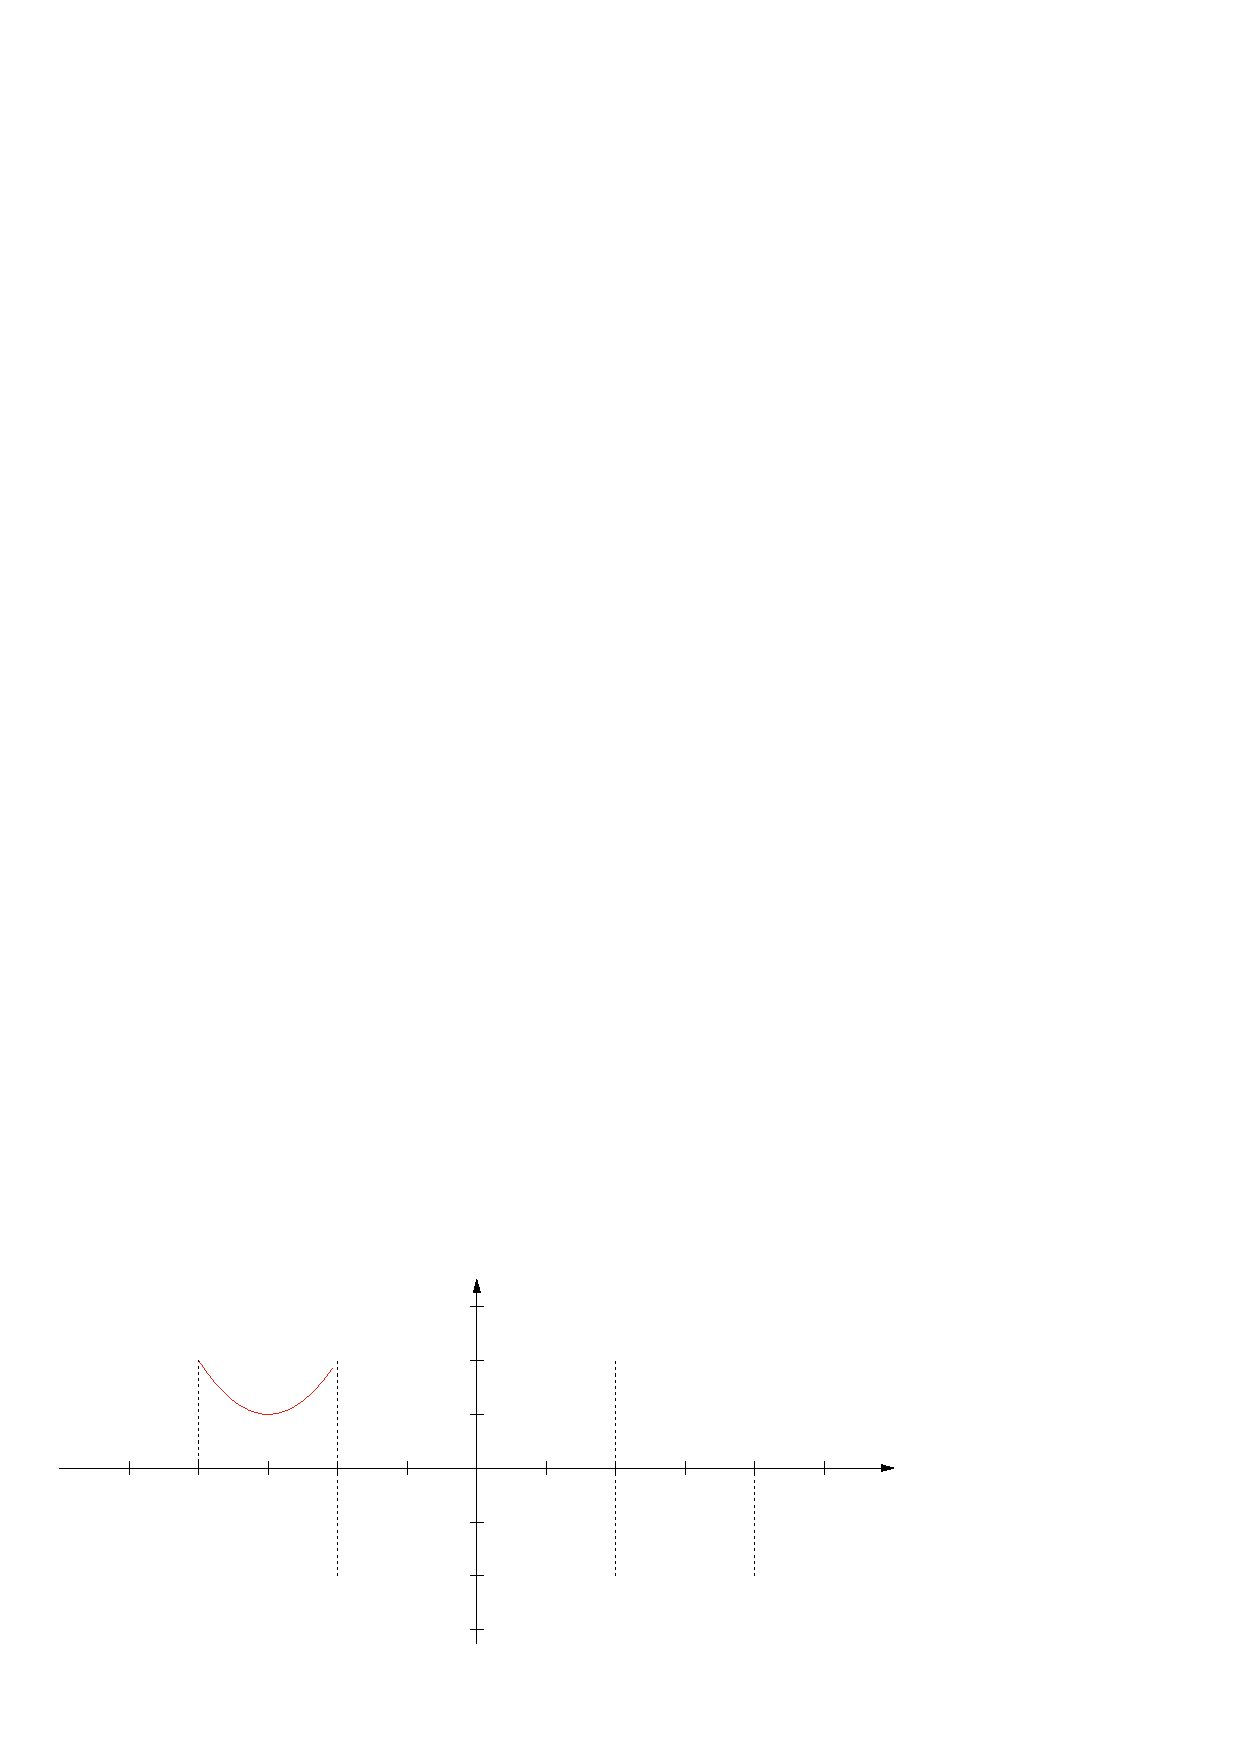
\includegraphics[width={360.00bp},height={172.80bp}]{figura_02_08}}%
    \gplfronttext
  \end{picture}%
\endgroup

\end{figure}

\subsection{Evaluación de coeficientes de \emph{Fourier}}
\subsubsection{Simetría de cuarto de onda par}
Como la función $f(t)$ tiene simetría de media onda:
\begin{equation}
    a_0=0
\end{equation}

Como la función $f(t)$ es una función par:
\begin{equation}
    b_n=0
\end{equation}

Como la función $f(t)$ tiene simetría de media onda: $a_n=0$ cuando $n$ es par.

Para $n$ impar:
\begin{equation*}
\begin{split}
    a_n
        &=\frac{4}{T}\int_0^{T/2}f(t)\cos(n\omega_0\,t)\,dt\\
        &=\frac{4}{T}\left[
            \int_0^{T/4}f(t)\cos(n\omega_0\,t)\,dt+
            \int_{T/4}^{T/2}f(t)\cos(n\omega_0\,t)\,dt
        \right]\\
        &=\frac{4}{T}\left[
            \int_0^{T/4}f(t)\cos(n\omega_0\,t)\,dt-
            \int_{T/4}^{T/2}f(t-\frac{T}{2})\cos(n\omega_0\,t)\,dt
        \right]\\
\end{split}
\end{equation*}
\begin{equation*}
    \tau=t-\frac{T}{2}
\end{equation*}
\begin{equation*}
    d\tau=dt
\end{equation*}
\begin{equation*}
\begin{split}
    a_n
        &=\frac{4}{T}\left[
            \int_0^{T/4}f(t)\cos(n\omega_0\,t)\,dt-
            \int_{\tau=T/4-T/2}^{\tau=T/2-T/2}
                f(\tau)\cos(n\omega_0(\tau+\frac{T}{2}))\,d\tau
        \right]\\
        &=\frac{4}{T}\left[
            \int_0^{T/4}f(t)\cos(n\omega_0\,t)\,dt-
            \int_{-T/4}^{0}f(\tau)\cos(n\omega_0(\tau+\frac{T}{2}))\,d\tau
        \right]\\
\end{split}
\end{equation*}
\begin{equation*}
\begin{split}
    n\omega_0(\tau+T/2)
        &=n\omega_0\tau+n\omega_0\frac{T}{2}\\
        &=n\omega_0\tau+n\frac{2\pi}{T}\frac{T}{2}\\
        &=n\omega_0\tau+n\pi\\
\end{split}
\end{equation*}
\begin{equation*}
\begin{split}
    \cos(n\omega_0\tau+n\pi)
        &=\cos(n\omega_0\tau)\cos(n\pi)-\sen(n\pi)\sen(n\omega_0\tau)\\
        &=\cos(n\omega_0\tau)\cos(n\pi)\\
        &=-\cos(n\omega_0\tau)\\
\end{split}
\end{equation*}
\begin{equation*}
\begin{split}
    a_n
        &=\frac{4}{T}\left[
            \int_0^{T/4}f(t)\cos(n\omega_0\,t)\,dt+
            \int_{-T/4}^0\,f(\tau)\cos(n\omega_0\tau)\,d\tau
        \right]\\
        &=\frac{4}{T}\left[\int_{-T/4}^{T/4}f(t)\cos(n\omega_0\,t)\,dt\right]\\
        &=\frac{4}{T}\left(2\int_0^{T/4}f(t)\cos(n\omega_0\,t)\,dt\right)\\
        &=\frac{8}{T}\int_0^{T/4}f(t)\cos(n\omega_0\,t)\,dt\\
\end{split}
\end{equation*}
\begin{equation}
\begin{cases}
    n:\text{par}&a_n=0\\
    n:\text{impar}&a_n=\frac{8}{T}\int_0^{T/4}f(t)\cos(n\omega_0\,t)\,dt\\
\end{cases}
\end{equation}

\subsubsection{Simetría de cuarto de onda impar}
Como la función $f(t)$ tiene simetría de media onda:
\begin{equation}
    a_0=0
\end{equation}

Como la función $f(t)$ es una función impar:
\begin{equation}
    a_n=0
\end{equation}

Como la función $f(t)$ tiene simetría de media onda: $b_n=0$ cuando $n$ es par.

Para $n$ impar:
\begin{equation*}
\begin{split}
    b_n
        &=\frac{4}{T}\int_0^{T/2}f(t)\sen(n\omega_0\,t)\,dt\\
        &=\frac{4}{T}\left[
            \int_0^{T/4}f(t)\sen(n\omega_0\,t)\,dt+
            \int_{T/4}^{T/2}f(t)\sen(n\omega_0\,t)\,dt
        \right]\\
        &=\frac{4}{T}\left[
            \int_0^{T/4}f(t)\sen(n\omega_0\,t)\,dt-
            \int_{T/4}^{T/2}f(t-\frac{T}{2})\sen(n\omega_0\,t)\,dt
        \right]\\
\end{split}
\end{equation*}
\begin{equation*}
    \tau=t-\frac{T}{2}
\end{equation*}
\begin{equation*}
    d\tau=dt
\end{equation*}
\begin{equation*}
\begin{split}
    b_n
        &=\frac{4}{T}\left[
            \int_0^{T/4}f(t)\sen(n\omega_0\,t)\,dt-
            \int_{\tau=T/4-T/2}^{\tau=T/2-T/2}
                f(\tau)\sen(n\omega_0(\tau+\frac{T}{2}))\,d\tau
        \right]\\
        &=\frac{4}{T}\left[
            \int_0^{T/4}f(t)\sen(n\omega_0\,t)\,dt-
            \int_{-T/4}^{0}
                f(\tau)\sen(n\omega_0(\tau+\frac{T}{2}))\,d\tau
        \right]\\
\end{split}
\end{equation*}
\begin{equation*}
\begin{split}
    n\omega_0(\tau+T/2)
        &=n\omega_0\tau+n\omega_0\frac{T}{2}\\
        &=n\omega_0\tau+n\frac{2\pi}{T}\frac{T}{2}\\
        &=n\omega_0\tau+n\pi\\
\end{split}
\end{equation*}
\begin{equation*}
\begin{split}
    \sen(n\omega_0\tau+n\pi)
        &=\sen(n\omega_0\tau)\cos(n\pi)+\sen(n\pi)\cos(n\omega_0\tau)\\
        &=\sen(n\omega_0\tau)\cos(n\pi)\\
        &=-\sen(n\omega_0\tau)\\
\end{split}
\end{equation*}
\begin{equation*}
\begin{split}
    b_n
        &=\frac{4}{T}\left[
            \int_0^{T/4}f(t)\sen(n\omega_0\,t)\,dt+
            \int_{-T/4}^0\,f(\tau)\sen(n\omega_0\tau)\,d\tau
        \right]\\
        &=\frac{4}{T}\left[\int_{-T/4}^{T/4}f(t)\sen(n\omega_0\,t)\,dt\right]\\
        &=\frac{4}{T}\left(2\int_0^{T/4}f(t)\sen(n\omega_0\,t)\,dt\right)\\
        &=\frac{8}{T}\int_0^{T/4}f(t)\sen(n\omega_0\,t)\,dt\\
\end{split}
\end{equation*}
\begin{equation}
\begin{cases}
    n:\text{par}&b_n=0\\
    n:\text{impar}&b_n=\frac{8}{T}\int_0^{T/4}f(t)\sen(n\omega_0\,t)\,dt\\
\end{cases}
\end{equation}

\section{Expansión periódica de funciones definidas en intervalos finitos}
Sea $f(t)$ una función no periódica:
\begin{figure}[H]
    \centering
    % GNUPLOT: LaTeX picture with Postscript
\begingroup
  \makeatletter
  \providecommand\color[2][]{%
    \GenericError{(gnuplot) \space\space\space\@spaces}{%
      Package color not loaded in conjunction with
      terminal option `colourtext'%
    }{See the gnuplot documentation for explanation.%
    }{Either use 'blacktext' in gnuplot or load the package
      color.sty in LaTeX.}%
    \renewcommand\color[2][]{}%
  }%
  \providecommand\includegraphics[2][]{%
    \GenericError{(gnuplot) \space\space\space\@spaces}{%
      Package graphicx or graphics not loaded%
    }{See the gnuplot documentation for explanation.%
    }{The gnuplot epslatex terminal needs graphicx.sty or graphics.sty.}%
    \renewcommand\includegraphics[2][]{}%
  }%
  \providecommand\rotatebox[2]{#2}%
  \@ifundefined{ifGPcolor}{%
    \newif\ifGPcolor
    \GPcolorfalse
  }{}%
  \@ifundefined{ifGPblacktext}{%
    \newif\ifGPblacktext
    \GPblacktexttrue
  }{}%
  % define a \g@addto@macro without @ in the name:
  \let\gplgaddtomacro\g@addto@macro
  % define empty templates for all commands taking text:
  \gdef\gplbacktext{}%
  \gdef\gplfronttext{}%
  \makeatother
  \ifGPblacktext
    % no textcolor at all
    \def\colorrgb#1{}%
    \def\colorgray#1{}%
  \else
    % gray or color?
    \ifGPcolor
      \def\colorrgb#1{\color[rgb]{#1}}%
      \def\colorgray#1{\color[gray]{#1}}%
      \expandafter\def\csname LTw\endcsname{\color{white}}%
      \expandafter\def\csname LTb\endcsname{\color{black}}%
      \expandafter\def\csname LTa\endcsname{\color{black}}%
      \expandafter\def\csname LT0\endcsname{\color[rgb]{1,0,0}}%
      \expandafter\def\csname LT1\endcsname{\color[rgb]{0,1,0}}%
      \expandafter\def\csname LT2\endcsname{\color[rgb]{0,0,1}}%
      \expandafter\def\csname LT3\endcsname{\color[rgb]{1,0,1}}%
      \expandafter\def\csname LT4\endcsname{\color[rgb]{0,1,1}}%
      \expandafter\def\csname LT5\endcsname{\color[rgb]{1,1,0}}%
      \expandafter\def\csname LT6\endcsname{\color[rgb]{0,0,0}}%
      \expandafter\def\csname LT7\endcsname{\color[rgb]{1,0.3,0}}%
      \expandafter\def\csname LT8\endcsname{\color[rgb]{0.5,0.5,0.5}}%
    \else
      % gray
      \def\colorrgb#1{\color{black}}%
      \def\colorgray#1{\color[gray]{#1}}%
      \expandafter\def\csname LTw\endcsname{\color{white}}%
      \expandafter\def\csname LTb\endcsname{\color{black}}%
      \expandafter\def\csname LTa\endcsname{\color{black}}%
      \expandafter\def\csname LT0\endcsname{\color{black}}%
      \expandafter\def\csname LT1\endcsname{\color{black}}%
      \expandafter\def\csname LT2\endcsname{\color{black}}%
      \expandafter\def\csname LT3\endcsname{\color{black}}%
      \expandafter\def\csname LT4\endcsname{\color{black}}%
      \expandafter\def\csname LT5\endcsname{\color{black}}%
      \expandafter\def\csname LT6\endcsname{\color{black}}%
      \expandafter\def\csname LT7\endcsname{\color{black}}%
      \expandafter\def\csname LT8\endcsname{\color{black}}%
    \fi
  \fi
    \setlength{\unitlength}{0.0500bp}%
    \ifx\gptboxheight\undefined%
      \newlength{\gptboxheight}%
      \newlength{\gptboxwidth}%
      \newsavebox{\gptboxtext}%
    \fi%
    \setlength{\fboxrule}{0.5pt}%
    \setlength{\fboxsep}{1pt}%
    \definecolor{tbcol}{rgb}{1,1,1}%
\begin{picture}(6336.00,2590.00)%
    \gplgaddtomacro\gplbacktext{%
      \csname LTb\endcsname%%
      \put(1233,416){\makebox(0,0)[r]{\strut{}}}%
      \put(1233,863){\makebox(0,0)[r]{\strut{}}}%
      \put(1233,1311){\makebox(0,0)[r]{\strut{}}}%
      \put(1233,1758){\makebox(0,0)[r]{\strut{}}}%
      \put(1233,2205){\makebox(0,0)[r]{\strut{}}}%
      \put(603,640){\makebox(0,0){\strut{}}}%
      \put(1329,640){\makebox(0,0){\strut{}}}%
      \put(2055,640){\makebox(0,0){\strut{}}}%
      \put(2781,640){\makebox(0,0){\strut{}}}%
      \put(3506,640){\makebox(0,0){\strut{}}}%
      \put(4232,640){\makebox(0,0){\strut{}}}%
      \put(4958,640){\makebox(0,0){\strut{}}}%
      \put(5684,640){\makebox(0,0){\strut{}}}%
      \csname LTb\endcsname%%
      \put(6228,863){\makebox(0,0)[l]{\strut{}$t$}}%
      \put(1502,2429){\makebox(0,0)[l]{\strut{}$f(t)$}}%
      \put(2681,662){\makebox(0,0)[l]{\strut{}$M$}}%
    }%
    \gplgaddtomacro\gplfronttext{%
    }%
    \gplbacktext
    \put(0,0){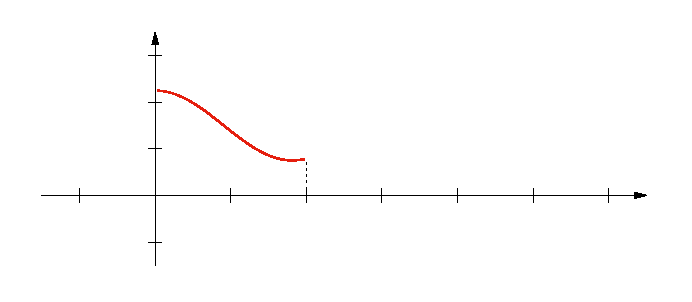
\includegraphics[width={316.80bp},height={129.50bp}]{figura_02_09}}%
    \gplfronttext
  \end{picture}%
\endgroup

\end{figure}

$f(t)$ se convierte en periódica al repetirla un intervalo $T\geq M$.
\begin{figure}[H]
    \centering
    % GNUPLOT: LaTeX picture with Postscript
\begingroup
  \makeatletter
  \providecommand\color[2][]{%
    \GenericError{(gnuplot) \space\space\space\@spaces}{%
      Package color not loaded in conjunction with
      terminal option `colourtext'%
    }{See the gnuplot documentation for explanation.%
    }{Either use 'blacktext' in gnuplot or load the package
      color.sty in LaTeX.}%
    \renewcommand\color[2][]{}%
  }%
  \providecommand\includegraphics[2][]{%
    \GenericError{(gnuplot) \space\space\space\@spaces}{%
      Package graphicx or graphics not loaded%
    }{See the gnuplot documentation for explanation.%
    }{The gnuplot epslatex terminal needs graphicx.sty or graphics.sty.}%
    \renewcommand\includegraphics[2][]{}%
  }%
  \providecommand\rotatebox[2]{#2}%
  \@ifundefined{ifGPcolor}{%
    \newif\ifGPcolor
    \GPcolorfalse
  }{}%
  \@ifundefined{ifGPblacktext}{%
    \newif\ifGPblacktext
    \GPblacktexttrue
  }{}%
  % define a \g@addto@macro without @ in the name:
  \let\gplgaddtomacro\g@addto@macro
  % define empty templates for all commands taking text:
  \gdef\gplbacktext{}%
  \gdef\gplfronttext{}%
  \makeatother
  \ifGPblacktext
    % no textcolor at all
    \def\colorrgb#1{}%
    \def\colorgray#1{}%
  \else
    % gray or color?
    \ifGPcolor
      \def\colorrgb#1{\color[rgb]{#1}}%
      \def\colorgray#1{\color[gray]{#1}}%
      \expandafter\def\csname LTw\endcsname{\color{white}}%
      \expandafter\def\csname LTb\endcsname{\color{black}}%
      \expandafter\def\csname LTa\endcsname{\color{black}}%
      \expandafter\def\csname LT0\endcsname{\color[rgb]{1,0,0}}%
      \expandafter\def\csname LT1\endcsname{\color[rgb]{0,1,0}}%
      \expandafter\def\csname LT2\endcsname{\color[rgb]{0,0,1}}%
      \expandafter\def\csname LT3\endcsname{\color[rgb]{1,0,1}}%
      \expandafter\def\csname LT4\endcsname{\color[rgb]{0,1,1}}%
      \expandafter\def\csname LT5\endcsname{\color[rgb]{1,1,0}}%
      \expandafter\def\csname LT6\endcsname{\color[rgb]{0,0,0}}%
      \expandafter\def\csname LT7\endcsname{\color[rgb]{1,0.3,0}}%
      \expandafter\def\csname LT8\endcsname{\color[rgb]{0.5,0.5,0.5}}%
    \else
      % gray
      \def\colorrgb#1{\color{black}}%
      \def\colorgray#1{\color[gray]{#1}}%
      \expandafter\def\csname LTw\endcsname{\color{white}}%
      \expandafter\def\csname LTb\endcsname{\color{black}}%
      \expandafter\def\csname LTa\endcsname{\color{black}}%
      \expandafter\def\csname LT0\endcsname{\color{black}}%
      \expandafter\def\csname LT1\endcsname{\color{black}}%
      \expandafter\def\csname LT2\endcsname{\color{black}}%
      \expandafter\def\csname LT3\endcsname{\color{black}}%
      \expandafter\def\csname LT4\endcsname{\color{black}}%
      \expandafter\def\csname LT5\endcsname{\color{black}}%
      \expandafter\def\csname LT6\endcsname{\color{black}}%
      \expandafter\def\csname LT7\endcsname{\color{black}}%
      \expandafter\def\csname LT8\endcsname{\color{black}}%
    \fi
  \fi
    \setlength{\unitlength}{0.0500bp}%
    \ifx\gptboxheight\undefined%
      \newlength{\gptboxheight}%
      \newlength{\gptboxwidth}%
      \newsavebox{\gptboxtext}%
    \fi%
    \setlength{\fboxrule}{0.5pt}%
    \setlength{\fboxsep}{1pt}%
    \definecolor{tbcol}{rgb}{1,1,1}%
\begin{picture}(6336.00,2590.00)%
    \gplgaddtomacro\gplbacktext{%
      \csname LTb\endcsname%%
      \put(1233,416){\makebox(0,0)[r]{\strut{}}}%
      \put(1233,863){\makebox(0,0)[r]{\strut{}}}%
      \put(1233,1311){\makebox(0,0)[r]{\strut{}}}%
      \put(1233,1758){\makebox(0,0)[r]{\strut{}}}%
      \put(1233,2205){\makebox(0,0)[r]{\strut{}}}%
      \put(603,640){\makebox(0,0){\strut{}}}%
      \put(1329,640){\makebox(0,0){\strut{}}}%
      \put(2055,640){\makebox(0,0){\strut{}}}%
      \put(2781,640){\makebox(0,0){\strut{}}}%
      \put(3506,640){\makebox(0,0){\strut{}}}%
      \put(4232,640){\makebox(0,0){\strut{}}}%
      \put(4958,640){\makebox(0,0){\strut{}}}%
      \put(5684,640){\makebox(0,0){\strut{}}}%
      \csname LTb\endcsname%%
      \put(6228,863){\makebox(0,0)[l]{\strut{}$t$}}%
      \put(1502,2429){\makebox(0,0)[l]{\strut{}$f(t)$}}%
      \put(2681,662){\makebox(0,0)[l]{\strut{}$M$}}%
      \put(2360,192){\makebox(0,0)[l]{\strut{}$T$}}%
    }%
    \gplgaddtomacro\gplfronttext{%
    }%
    \gplgaddtomacro\gplbacktext{%
      \csname LTb\endcsname%%
      \put(1233,416){\makebox(0,0)[r]{\strut{}}}%
      \put(1233,863){\makebox(0,0)[r]{\strut{}}}%
      \put(1233,1311){\makebox(0,0)[r]{\strut{}}}%
      \put(1233,1758){\makebox(0,0)[r]{\strut{}}}%
      \put(1233,2205){\makebox(0,0)[r]{\strut{}}}%
      \put(603,640){\makebox(0,0){\strut{}}}%
      \put(1329,640){\makebox(0,0){\strut{}}}%
      \put(2055,640){\makebox(0,0){\strut{}}}%
      \put(2781,640){\makebox(0,0){\strut{}}}%
      \put(3506,640){\makebox(0,0){\strut{}}}%
      \put(4232,640){\makebox(0,0){\strut{}}}%
      \put(4958,640){\makebox(0,0){\strut{}}}%
      \put(5684,640){\makebox(0,0){\strut{}}}%
      \csname LTb\endcsname%%
      \put(6228,863){\makebox(0,0)[l]{\strut{}$t$}}%
      \put(1502,2429){\makebox(0,0)[l]{\strut{}$f(t)$}}%
      \put(2681,662){\makebox(0,0)[l]{\strut{}$M$}}%
      \put(2360,192){\makebox(0,0)[l]{\strut{}$T$}}%
    }%
    \gplgaddtomacro\gplfronttext{%
    }%
    \gplgaddtomacro\gplbacktext{%
      \csname LTb\endcsname%%
      \put(1233,416){\makebox(0,0)[r]{\strut{}}}%
      \put(1233,863){\makebox(0,0)[r]{\strut{}}}%
      \put(1233,1311){\makebox(0,0)[r]{\strut{}}}%
      \put(1233,1758){\makebox(0,0)[r]{\strut{}}}%
      \put(1233,2205){\makebox(0,0)[r]{\strut{}}}%
      \put(603,640){\makebox(0,0){\strut{}}}%
      \put(1329,640){\makebox(0,0){\strut{}}}%
      \put(2055,640){\makebox(0,0){\strut{}}}%
      \put(2781,640){\makebox(0,0){\strut{}}}%
      \put(3506,640){\makebox(0,0){\strut{}}}%
      \put(4232,640){\makebox(0,0){\strut{}}}%
      \put(4958,640){\makebox(0,0){\strut{}}}%
      \put(5684,640){\makebox(0,0){\strut{}}}%
      \csname LTb\endcsname%%
      \put(6228,863){\makebox(0,0)[l]{\strut{}$t$}}%
      \put(1502,2429){\makebox(0,0)[l]{\strut{}$f(t)$}}%
      \put(2681,662){\makebox(0,0)[l]{\strut{}$M$}}%
      \put(2360,192){\makebox(0,0)[l]{\strut{}$T$}}%
    }%
    \gplgaddtomacro\gplfronttext{%
    }%
    \gplgaddtomacro\gplbacktext{%
      \csname LTb\endcsname%%
      \put(1233,416){\makebox(0,0)[r]{\strut{}}}%
      \put(1233,863){\makebox(0,0)[r]{\strut{}}}%
      \put(1233,1311){\makebox(0,0)[r]{\strut{}}}%
      \put(1233,1758){\makebox(0,0)[r]{\strut{}}}%
      \put(1233,2205){\makebox(0,0)[r]{\strut{}}}%
      \put(603,640){\makebox(0,0){\strut{}}}%
      \put(1329,640){\makebox(0,0){\strut{}}}%
      \put(2055,640){\makebox(0,0){\strut{}}}%
      \put(2781,640){\makebox(0,0){\strut{}}}%
      \put(3506,640){\makebox(0,0){\strut{}}}%
      \put(4232,640){\makebox(0,0){\strut{}}}%
      \put(4958,640){\makebox(0,0){\strut{}}}%
      \put(5684,640){\makebox(0,0){\strut{}}}%
      \csname LTb\endcsname%%
      \put(6228,863){\makebox(0,0)[l]{\strut{}$t$}}%
      \put(1502,2429){\makebox(0,0)[l]{\strut{}$f(t)$}}%
      \put(2681,662){\makebox(0,0)[l]{\strut{}$M$}}%
      \put(2360,192){\makebox(0,0)[l]{\strut{}$T$}}%
    }%
    \gplgaddtomacro\gplfronttext{%
    }%
    \gplbacktext
    \put(0,0){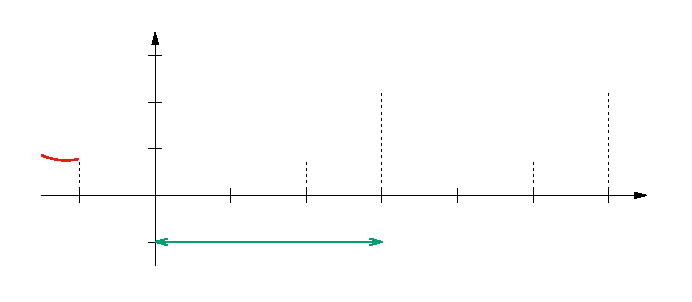
\includegraphics[width={316.80bp},height={129.50bp}]{figura_02_10}}%
    \gplfronttext
  \end{picture}%
\endgroup

\end{figure}

$f(t)$ puede expandirse periódicamente asignando alguna simetría conocida.


\chapter{Serie compleja de \emph{Fourier} y espectros discretos de frecuencia}

\section{Números complejos}

\begin{figure}[H]
    \centering
    % GNUPLOT: LaTeX picture with Postscript
\begingroup
  \makeatletter
  \providecommand\color[2][]{%
    \GenericError{(gnuplot) \space\space\space\@spaces}{%
      Package color not loaded in conjunction with
      terminal option `colourtext'%
    }{See the gnuplot documentation for explanation.%
    }{Either use 'blacktext' in gnuplot or load the package
      color.sty in LaTeX.}%
    \renewcommand\color[2][]{}%
  }%
  \providecommand\includegraphics[2][]{%
    \GenericError{(gnuplot) \space\space\space\@spaces}{%
      Package graphicx or graphics not loaded%
    }{See the gnuplot documentation for explanation.%
    }{The gnuplot epslatex terminal needs graphicx.sty or graphics.sty.}%
    \renewcommand\includegraphics[2][]{}%
  }%
  \providecommand\rotatebox[2]{#2}%
  \@ifundefined{ifGPcolor}{%
    \newif\ifGPcolor
    \GPcolorfalse
  }{}%
  \@ifundefined{ifGPblacktext}{%
    \newif\ifGPblacktext
    \GPblacktexttrue
  }{}%
  % define a \g@addto@macro without @ in the name:
  \let\gplgaddtomacro\g@addto@macro
  % define empty templates for all commands taking text:
  \gdef\gplbacktext{}%
  \gdef\gplfronttext{}%
  \makeatother
  \ifGPblacktext
    % no textcolor at all
    \def\colorrgb#1{}%
    \def\colorgray#1{}%
  \else
    % gray or color?
    \ifGPcolor
      \def\colorrgb#1{\color[rgb]{#1}}%
      \def\colorgray#1{\color[gray]{#1}}%
      \expandafter\def\csname LTw\endcsname{\color{white}}%
      \expandafter\def\csname LTb\endcsname{\color{black}}%
      \expandafter\def\csname LTa\endcsname{\color{black}}%
      \expandafter\def\csname LT0\endcsname{\color[rgb]{1,0,0}}%
      \expandafter\def\csname LT1\endcsname{\color[rgb]{0,1,0}}%
      \expandafter\def\csname LT2\endcsname{\color[rgb]{0,0,1}}%
      \expandafter\def\csname LT3\endcsname{\color[rgb]{1,0,1}}%
      \expandafter\def\csname LT4\endcsname{\color[rgb]{0,1,1}}%
      \expandafter\def\csname LT5\endcsname{\color[rgb]{1,1,0}}%
      \expandafter\def\csname LT6\endcsname{\color[rgb]{0,0,0}}%
      \expandafter\def\csname LT7\endcsname{\color[rgb]{1,0.3,0}}%
      \expandafter\def\csname LT8\endcsname{\color[rgb]{0.5,0.5,0.5}}%
    \else
      % gray
      \def\colorrgb#1{\color{black}}%
      \def\colorgray#1{\color[gray]{#1}}%
      \expandafter\def\csname LTw\endcsname{\color{white}}%
      \expandafter\def\csname LTb\endcsname{\color{black}}%
      \expandafter\def\csname LTa\endcsname{\color{black}}%
      \expandafter\def\csname LT0\endcsname{\color{black}}%
      \expandafter\def\csname LT1\endcsname{\color{black}}%
      \expandafter\def\csname LT2\endcsname{\color{black}}%
      \expandafter\def\csname LT3\endcsname{\color{black}}%
      \expandafter\def\csname LT4\endcsname{\color{black}}%
      \expandafter\def\csname LT5\endcsname{\color{black}}%
      \expandafter\def\csname LT6\endcsname{\color{black}}%
      \expandafter\def\csname LT7\endcsname{\color{black}}%
      \expandafter\def\csname LT8\endcsname{\color{black}}%
    \fi
  \fi
    \setlength{\unitlength}{0.0500bp}%
    \ifx\gptboxheight\undefined%
      \newlength{\gptboxheight}%
      \newlength{\gptboxwidth}%
      \newsavebox{\gptboxtext}%
    \fi%
    \setlength{\fboxrule}{0.5pt}%
    \setlength{\fboxsep}{1pt}%
    \definecolor{tbcol}{rgb}{1,1,1}%
\begin{picture}(2880.00,2880.00)%
    \gplgaddtomacro\gplbacktext{%
      \csname LTb\endcsname%%
      \put(614,192){\makebox(0,0)[r]{\strut{}}}%
      \put(614,697){\makebox(0,0)[r]{\strut{}}}%
      \put(614,1203){\makebox(0,0)[r]{\strut{}}}%
      \put(614,1708){\makebox(0,0)[r]{\strut{}}}%
      \put(614,2214){\makebox(0,0)[r]{\strut{}}}%
      \put(614,2719){\makebox(0,0)[r]{\strut{}}}%
      \put(240,474){\makebox(0,0){\strut{}}}%
      \put(710,474){\makebox(0,0){\strut{}}}%
      \put(1180,474){\makebox(0,0){\strut{}}}%
      \put(1651,474){\makebox(0,0){\strut{}}}%
      \put(2121,474){\makebox(0,0){\strut{}}}%
      \put(2591,474){\makebox(0,0){\strut{}}}%
      \csname LTb\endcsname%%
      \put(3061,697){\makebox(0,0)[l]{\strut{}$\mathbb{R}e$}}%
      \put(875,2845){\makebox(0,0)[l]{\strut{}$\mathbb{I}m$}}%
      \put(1886,2441){\makebox(0,0)[l]{\strut{}$z=a+jb$}}%
      \put(2074,521){\makebox(0,0)[l]{\strut{}$a$}}%
      \put(358,2239){\makebox(0,0)[l]{\strut{}$jb$}}%
      \put(1274,900){\makebox(0,0)[l]{\strut{}$\theta$}}%
    }%
    \gplgaddtomacro\gplfronttext{%
    }%
    \gplgaddtomacro\gplbacktext{%
      \csname LTb\endcsname%%
      \put(614,192){\makebox(0,0)[r]{\strut{}}}%
      \put(614,697){\makebox(0,0)[r]{\strut{}}}%
      \put(614,1203){\makebox(0,0)[r]{\strut{}}}%
      \put(614,1708){\makebox(0,0)[r]{\strut{}}}%
      \put(614,2214){\makebox(0,0)[r]{\strut{}}}%
      \put(614,2719){\makebox(0,0)[r]{\strut{}}}%
      \put(240,474){\makebox(0,0){\strut{}}}%
      \put(710,474){\makebox(0,0){\strut{}}}%
      \put(1180,474){\makebox(0,0){\strut{}}}%
      \put(1651,474){\makebox(0,0){\strut{}}}%
      \put(2121,474){\makebox(0,0){\strut{}}}%
      \put(2591,474){\makebox(0,0){\strut{}}}%
      \csname LTb\endcsname%%
      \put(3061,697){\makebox(0,0)[l]{\strut{}$\mathbb{R}e$}}%
      \put(875,2845){\makebox(0,0)[l]{\strut{}$\mathbb{I}m$}}%
      \put(1886,2441){\makebox(0,0)[l]{\strut{}$z=a+jb$}}%
      \put(2074,521){\makebox(0,0)[l]{\strut{}$a$}}%
      \put(358,2239){\makebox(0,0)[l]{\strut{}$jb$}}%
      \put(1274,900){\makebox(0,0)[l]{\strut{}$\theta$}}%
    }%
    \gplgaddtomacro\gplfronttext{%
    }%
    \gplbacktext
    \put(0,0){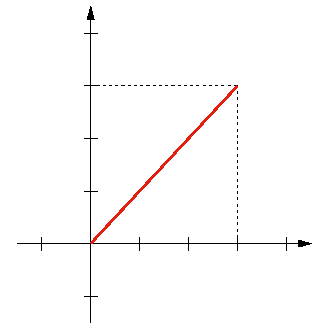
\includegraphics[width={144.00bp},height={144.00bp}]{figura_03_01}}%
    \gplfronttext
  \end{picture}%
\endgroup

\end{figure}

\begin{center}
    Unidad imaginaria: $i=j=\sqrt{-1}$\\
    Forma rectangular: $z=a+jb$\\
    Módulo: $|z|=\sqrt{a^2+b^2}$\\
    Argumento: $\theta=\arctan(\frac{b}{a})$\\
\end{center}

Forma polar:
\begin{equation*}
    z=|z|\cos(\theta)+j|z|\sen(\theta)
        =|z|(\cos(\theta)+j\sen(\theta))
\end{equation*}

Formula de \emph{Euler}:
\begin{equation}
    e^{j\theta}=\cos(\theta)+j\sen(\theta)
\end{equation}

Por tanto:
\begin{equation*}
    z=|z|e^{j\theta}
\end{equation*}

Forma exponencial o fasorial:
\begin{equation*}
    z=|z|\angle\theta
\end{equation*}

\subsection{Formas complejas del seno y coseno}

\begin{equation}
    e^{j\theta}=\cos(\theta)+j\sen(\theta)
    \label{e1}
\end{equation}
\begin{equation}
    e^{-j\theta}=\cos(\theta)-j\sen(\theta)
    \label{e2}
\end{equation}

Sumando las ecuaciones~\ref{e1} y~\ref{e2}:
\begin{equation*}
    e^{j\theta}+e^{-j\theta}=2\cos(\theta)
\end{equation*}
\begin{equation}
    \cos(\theta)=\frac{e^{j\theta}+e^{-j\theta}}{2}
\end{equation}

Restando las ecuaciones~\ref{e1} y~\ref{e2}:
\begin{equation*}
    e^{j\theta}-e^{-j\theta}=2j\sen(\theta)
\end{equation*}
\begin{equation}
    \sen(\theta)=\frac{e^{j\theta}-e^{-j\theta}}{2j}
\end{equation}

\subsection{Conjugado}

\begin{figure}[H]
    \centering
    % GNUPLOT: LaTeX picture with Postscript
\begingroup
  \makeatletter
  \providecommand\color[2][]{%
    \GenericError{(gnuplot) \space\space\space\@spaces}{%
      Package color not loaded in conjunction with
      terminal option `colourtext'%
    }{See the gnuplot documentation for explanation.%
    }{Either use 'blacktext' in gnuplot or load the package
      color.sty in LaTeX.}%
    \renewcommand\color[2][]{}%
  }%
  \providecommand\includegraphics[2][]{%
    \GenericError{(gnuplot) \space\space\space\@spaces}{%
      Package graphicx or graphics not loaded%
    }{See the gnuplot documentation for explanation.%
    }{The gnuplot epslatex terminal needs graphicx.sty or graphics.sty.}%
    \renewcommand\includegraphics[2][]{}%
  }%
  \providecommand\rotatebox[2]{#2}%
  \@ifundefined{ifGPcolor}{%
    \newif\ifGPcolor
    \GPcolorfalse
  }{}%
  \@ifundefined{ifGPblacktext}{%
    \newif\ifGPblacktext
    \GPblacktexttrue
  }{}%
  % define a \g@addto@macro without @ in the name:
  \let\gplgaddtomacro\g@addto@macro
  % define empty templates for all commands taking text:
  \gdef\gplbacktext{}%
  \gdef\gplfronttext{}%
  \makeatother
  \ifGPblacktext
    % no textcolor at all
    \def\colorrgb#1{}%
    \def\colorgray#1{}%
  \else
    % gray or color?
    \ifGPcolor
      \def\colorrgb#1{\color[rgb]{#1}}%
      \def\colorgray#1{\color[gray]{#1}}%
      \expandafter\def\csname LTw\endcsname{\color{white}}%
      \expandafter\def\csname LTb\endcsname{\color{black}}%
      \expandafter\def\csname LTa\endcsname{\color{black}}%
      \expandafter\def\csname LT0\endcsname{\color[rgb]{1,0,0}}%
      \expandafter\def\csname LT1\endcsname{\color[rgb]{0,1,0}}%
      \expandafter\def\csname LT2\endcsname{\color[rgb]{0,0,1}}%
      \expandafter\def\csname LT3\endcsname{\color[rgb]{1,0,1}}%
      \expandafter\def\csname LT4\endcsname{\color[rgb]{0,1,1}}%
      \expandafter\def\csname LT5\endcsname{\color[rgb]{1,1,0}}%
      \expandafter\def\csname LT6\endcsname{\color[rgb]{0,0,0}}%
      \expandafter\def\csname LT7\endcsname{\color[rgb]{1,0.3,0}}%
      \expandafter\def\csname LT8\endcsname{\color[rgb]{0.5,0.5,0.5}}%
    \else
      % gray
      \def\colorrgb#1{\color{black}}%
      \def\colorgray#1{\color[gray]{#1}}%
      \expandafter\def\csname LTw\endcsname{\color{white}}%
      \expandafter\def\csname LTb\endcsname{\color{black}}%
      \expandafter\def\csname LTa\endcsname{\color{black}}%
      \expandafter\def\csname LT0\endcsname{\color{black}}%
      \expandafter\def\csname LT1\endcsname{\color{black}}%
      \expandafter\def\csname LT2\endcsname{\color{black}}%
      \expandafter\def\csname LT3\endcsname{\color{black}}%
      \expandafter\def\csname LT4\endcsname{\color{black}}%
      \expandafter\def\csname LT5\endcsname{\color{black}}%
      \expandafter\def\csname LT6\endcsname{\color{black}}%
      \expandafter\def\csname LT7\endcsname{\color{black}}%
      \expandafter\def\csname LT8\endcsname{\color{black}}%
    \fi
  \fi
    \setlength{\unitlength}{0.0500bp}%
    \ifx\gptboxheight\undefined%
      \newlength{\gptboxheight}%
      \newlength{\gptboxwidth}%
      \newsavebox{\gptboxtext}%
    \fi%
    \setlength{\fboxrule}{0.5pt}%
    \setlength{\fboxsep}{1pt}%
    \definecolor{tbcol}{rgb}{1,1,1}%
\begin{picture}(3600.00,3600.00)%
    \gplgaddtomacro\gplbacktext{%
      \csname LTb\endcsname%%
      \put(1680,192){\makebox(0,0)[r]{\strut{}}}%
      \put(1680,598){\makebox(0,0)[r]{\strut{}}}%
      \put(1680,1004){\makebox(0,0)[r]{\strut{}}}%
      \put(1680,1410){\makebox(0,0)[r]{\strut{}}}%
      \put(1680,1816){\makebox(0,0)[r]{\strut{}}}%
      \put(1680,2221){\makebox(0,0)[r]{\strut{}}}%
      \put(1680,2627){\makebox(0,0)[r]{\strut{}}}%
      \put(1680,3033){\makebox(0,0)[r]{\strut{}}}%
      \put(1680,3439){\makebox(0,0)[r]{\strut{}}}%
      \put(240,1593){\makebox(0,0){\strut{}}}%
      \put(624,1593){\makebox(0,0){\strut{}}}%
      \put(1008,1593){\makebox(0,0){\strut{}}}%
      \put(1392,1593){\makebox(0,0){\strut{}}}%
      \put(1776,1593){\makebox(0,0){\strut{}}}%
      \put(2159,1593){\makebox(0,0){\strut{}}}%
      \put(2543,1593){\makebox(0,0){\strut{}}}%
      \put(2927,1593){\makebox(0,0){\strut{}}}%
      \put(3311,1593){\makebox(0,0){\strut{}}}%
      \csname LTb\endcsname%%
      \put(3695,1816){\makebox(0,0)[l]{\strut{}$\mathbb{R}e$}}%
      \put(1910,3540){\makebox(0,0)[l]{\strut{}$\mathbb{I}m$}}%
      \put(2927,3216){\makebox(0,0)[l]{\strut{}$z$}}%
      \put(2927,415){\makebox(0,0)[l]{\strut{}$z*$}}%
      \put(2889,1673){\makebox(0,0)[l]{\strut{}$a$}}%
      \put(1488,3053){\makebox(0,0)[l]{\strut{}$jb$}}%
      \put(1392,578){\makebox(0,0)[l]{\strut{}$-jb$}}%
      \put(2236,1978){\makebox(0,0)[l]{\strut{}$\theta$}}%
      \put(2236,1572){\makebox(0,0)[l]{\strut{}$-\theta$}}%
    }%
    \gplgaddtomacro\gplfronttext{%
    }%
    \gplgaddtomacro\gplbacktext{%
      \csname LTb\endcsname%%
      \put(1680,192){\makebox(0,0)[r]{\strut{}}}%
      \put(1680,598){\makebox(0,0)[r]{\strut{}}}%
      \put(1680,1004){\makebox(0,0)[r]{\strut{}}}%
      \put(1680,1410){\makebox(0,0)[r]{\strut{}}}%
      \put(1680,1816){\makebox(0,0)[r]{\strut{}}}%
      \put(1680,2221){\makebox(0,0)[r]{\strut{}}}%
      \put(1680,2627){\makebox(0,0)[r]{\strut{}}}%
      \put(1680,3033){\makebox(0,0)[r]{\strut{}}}%
      \put(1680,3439){\makebox(0,0)[r]{\strut{}}}%
      \put(240,1593){\makebox(0,0){\strut{}}}%
      \put(624,1593){\makebox(0,0){\strut{}}}%
      \put(1008,1593){\makebox(0,0){\strut{}}}%
      \put(1392,1593){\makebox(0,0){\strut{}}}%
      \put(1776,1593){\makebox(0,0){\strut{}}}%
      \put(2159,1593){\makebox(0,0){\strut{}}}%
      \put(2543,1593){\makebox(0,0){\strut{}}}%
      \put(2927,1593){\makebox(0,0){\strut{}}}%
      \put(3311,1593){\makebox(0,0){\strut{}}}%
      \csname LTb\endcsname%%
      \put(3695,1816){\makebox(0,0)[l]{\strut{}$\mathbb{R}e$}}%
      \put(1910,3540){\makebox(0,0)[l]{\strut{}$\mathbb{I}m$}}%
      \put(2927,3216){\makebox(0,0)[l]{\strut{}$z$}}%
      \put(2927,415){\makebox(0,0)[l]{\strut{}$z*$}}%
      \put(2889,1673){\makebox(0,0)[l]{\strut{}$a$}}%
      \put(1488,3053){\makebox(0,0)[l]{\strut{}$jb$}}%
      \put(1392,578){\makebox(0,0)[l]{\strut{}$-jb$}}%
      \put(2236,1978){\makebox(0,0)[l]{\strut{}$\theta$}}%
      \put(2236,1572){\makebox(0,0)[l]{\strut{}$-\theta$}}%
    }%
    \gplgaddtomacro\gplfronttext{%
    }%
    \gplgaddtomacro\gplbacktext{%
      \csname LTb\endcsname%%
      \put(1680,192){\makebox(0,0)[r]{\strut{}}}%
      \put(1680,598){\makebox(0,0)[r]{\strut{}}}%
      \put(1680,1004){\makebox(0,0)[r]{\strut{}}}%
      \put(1680,1410){\makebox(0,0)[r]{\strut{}}}%
      \put(1680,1816){\makebox(0,0)[r]{\strut{}}}%
      \put(1680,2221){\makebox(0,0)[r]{\strut{}}}%
      \put(1680,2627){\makebox(0,0)[r]{\strut{}}}%
      \put(1680,3033){\makebox(0,0)[r]{\strut{}}}%
      \put(1680,3439){\makebox(0,0)[r]{\strut{}}}%
      \put(240,1593){\makebox(0,0){\strut{}}}%
      \put(624,1593){\makebox(0,0){\strut{}}}%
      \put(1008,1593){\makebox(0,0){\strut{}}}%
      \put(1392,1593){\makebox(0,0){\strut{}}}%
      \put(1776,1593){\makebox(0,0){\strut{}}}%
      \put(2159,1593){\makebox(0,0){\strut{}}}%
      \put(2543,1593){\makebox(0,0){\strut{}}}%
      \put(2927,1593){\makebox(0,0){\strut{}}}%
      \put(3311,1593){\makebox(0,0){\strut{}}}%
      \csname LTb\endcsname%%
      \put(3695,1816){\makebox(0,0)[l]{\strut{}$\mathbb{R}e$}}%
      \put(1910,3540){\makebox(0,0)[l]{\strut{}$\mathbb{I}m$}}%
      \put(2927,3216){\makebox(0,0)[l]{\strut{}$z$}}%
      \put(2927,415){\makebox(0,0)[l]{\strut{}$z*$}}%
      \put(2889,1673){\makebox(0,0)[l]{\strut{}$a$}}%
      \put(1488,3053){\makebox(0,0)[l]{\strut{}$jb$}}%
      \put(1392,578){\makebox(0,0)[l]{\strut{}$-jb$}}%
      \put(2236,1978){\makebox(0,0)[l]{\strut{}$\theta$}}%
      \put(2236,1572){\makebox(0,0)[l]{\strut{}$-\theta$}}%
    }%
    \gplgaddtomacro\gplfronttext{%
    }%
    \gplgaddtomacro\gplbacktext{%
      \csname LTb\endcsname%%
      \put(1680,192){\makebox(0,0)[r]{\strut{}}}%
      \put(1680,598){\makebox(0,0)[r]{\strut{}}}%
      \put(1680,1004){\makebox(0,0)[r]{\strut{}}}%
      \put(1680,1410){\makebox(0,0)[r]{\strut{}}}%
      \put(1680,1816){\makebox(0,0)[r]{\strut{}}}%
      \put(1680,2221){\makebox(0,0)[r]{\strut{}}}%
      \put(1680,2627){\makebox(0,0)[r]{\strut{}}}%
      \put(1680,3033){\makebox(0,0)[r]{\strut{}}}%
      \put(1680,3439){\makebox(0,0)[r]{\strut{}}}%
      \put(240,1593){\makebox(0,0){\strut{}}}%
      \put(624,1593){\makebox(0,0){\strut{}}}%
      \put(1008,1593){\makebox(0,0){\strut{}}}%
      \put(1392,1593){\makebox(0,0){\strut{}}}%
      \put(1776,1593){\makebox(0,0){\strut{}}}%
      \put(2159,1593){\makebox(0,0){\strut{}}}%
      \put(2543,1593){\makebox(0,0){\strut{}}}%
      \put(2927,1593){\makebox(0,0){\strut{}}}%
      \put(3311,1593){\makebox(0,0){\strut{}}}%
      \csname LTb\endcsname%%
      \put(3695,1816){\makebox(0,0)[l]{\strut{}$\mathbb{R}e$}}%
      \put(1910,3540){\makebox(0,0)[l]{\strut{}$\mathbb{I}m$}}%
      \put(2927,3216){\makebox(0,0)[l]{\strut{}$z$}}%
      \put(2927,415){\makebox(0,0)[l]{\strut{}$z*$}}%
      \put(2889,1673){\makebox(0,0)[l]{\strut{}$a$}}%
      \put(1488,3053){\makebox(0,0)[l]{\strut{}$jb$}}%
      \put(1392,578){\makebox(0,0)[l]{\strut{}$-jb$}}%
      \put(2236,1978){\makebox(0,0)[l]{\strut{}$\theta$}}%
      \put(2236,1572){\makebox(0,0)[l]{\strut{}$-\theta$}}%
    }%
    \gplgaddtomacro\gplfronttext{%
    }%
    \gplbacktext
    \put(0,0){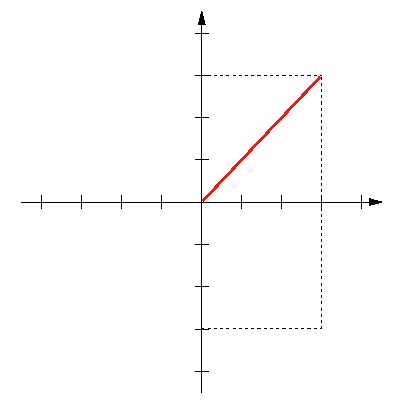
\includegraphics[width={180.00bp},height={180.00bp}]{figura_03_02}}%
    \gplfronttext
  \end{picture}%
\endgroup

\end{figure}

\begin{equation*}
    z=a+jb=|z|\angle\theta
\end{equation*}
\begin{equation*}
    z*=a-jb=|z|\angle-\theta
\end{equation*}
\begin{equation*}
    (z)(z*)={|z|}^2
\end{equation*}

\section{Serie compleja de \emph{Fourier}}
Partiendo de la serie trigonométrica de \emph{Fourier}:

\begin{equation*}
    f(t)=\frac{a_0}{2}+
    \sum_{n=1}^{\infty}\left[
        a_n\cos(n\omega_0 t)+
        b_n\sen(n\omega_0 t)
    \right]
\end{equation*}
\begin{equation*}
    f(t)=\frac{a_0}{2}+
    \sum_{n=1}^{\infty}\left[
        a_n\left(
            \frac{e^{jn\omega_0 t}+e^{-jn\omega_0 t}
            }{2}
        \right)+
        b_n\left(
            \frac{e^{jn\omega_0 t}+e^{-jn\omega_0 t}
            }{2j}
        \right)
    \right]
\end{equation*}
\begin{equation*}
    \frac{1}{j}=-j
\end{equation*}
\begin{equation*}
    f(t)=\frac{a_0}{2}+
    \sum_{n=1}^{\infty}\left[
        a_n\left(
            \frac{e^{jn\omega_0 t}+e^{-jn\omega_0 t}
            }{2}
        \right)-
        jb_n\left(
            \frac{e^{jn\omega_0 t}+e^{-jn\omega_0 t}
            }{2}
        \right)
    \right]
\end{equation*}
\begin{equation*}
    f(t)=\frac{a_0}{2}+
    \sum_{n=1}^{\infty}\left[
        \left(\frac{a_n-jb_n}{2}\right)e^{jn\omega_0 t}+
        \left(\frac{a_n+jb_n}{2}\right)e^{-jn\omega_0 t}
    \right]
\end{equation*}
\begin{equation*}
    f(t)=\frac{a_0}{2}+
    \sum_{n=1}^{\infty}\left[
        \left(\frac{a_n-jb_n}{2}\right)e^{jn\omega_0 t}
    \right]+
    \sum_{n=1}^{\infty}\left[
        \left(\frac{a_n+jb_n}{2}\right)e^{-jn\omega_0 t}
    \right]
\end{equation*}
\begin{equation*}
    f(t)=\frac{a_0}{2}+
    \sum_{n=1}^{\infty}\left[
        \left(\frac{a_n-jb_n}{2}\right)e^{jn\omega_0 t}
    \right]+
    \sum_{-n=1}^{\infty}\left[
        \left(\frac{a_{-n}+jb_{-n}}{2}\right)e^{jn\omega_0 t}
    \right]
\end{equation*}
\begin{equation*}
    f(t)=\frac{a_0}{2}+
    \sum_{n=1}^{\infty}\left[
        \left(\frac{a_n-jb_n}{2}\right)e^{jn\omega_0 t}
    \right]+
    \sum_{n=-1}^{-\infty}\left[
        \left(\frac{a_n+jb_n}{2}\right)e^{jn\omega_0 t}
    \right]
\end{equation*}
\begin{equation*}
    f(t)=\frac{a_0}{2}+
    \sum_{\substack{n=-\infty\\n\neq0}}^{\infty}\left(\frac{a_n-jb_n}{2}\right)e^{jn\omega_0 t}
\end{equation*}

Sean los coeficientes complejos de \emph{Fourier}:

\begin{equation*}
    c_n=\frac{a_n-jb_n}{2}
\end{equation*}
\begin{equation*}
    c_0=\frac{a_0}{2}
\end{equation*}

Entonces:

\begin{equation*}
    f(t)=c_0+\sum_{\substack{n=-\infty\\n\neq0}}^{\infty}c_n e^{jn\omega_0 t}
\end{equation*}
\begin{equation}
    f(t)=\sum_{n=-\infty}^{\infty}c_n e^{jn\omega_0 t}
\end{equation}

\subsection{Evaluación del coeficiente complejo de \emph{Fourier}}

\begin{equation*}
\begin{split}
    c_n
        &=\frac{a_n-jb_n}{2}\\
        &=\frac{1}{2}\left[\frac{2}{T}\int_0^T f(t)\cos(n\omega_0 t)\,dt-j\frac{2}{T}\int_0^T f(t)\sen(n\omega_0 t)\,dt\right]\\
        &=\frac{1}{T}\int_0^T f(t)\left[\cos(n\omega_0 t)-j\sen(n\omega_0 t)\right]dt\\
        &=\frac{1}{T}\int_0^T f(t)\,e^{-jn\omega_0 t}\,dt\\
\end{split}
\end{equation*}
\begin{equation}
    c_n=\frac{1}{T}\int_0^T f(t)\,e^{-jn\omega_0 t}\,dt
\end{equation}

En particular:

\begin{equation}
    c_0=\frac{1}{T}\int_0^T f(t)\,dt
\end{equation}

\subsection{Relación entre el coeficiente complejo y los coeficientes trigonométricos}

\begin{equation*}
    c_n=\frac{a_n-jbn}{2}
        =\frac{a_n}{2}+j\frac{-b_n}{2}
\end{equation*}

\begin{equation*}
    \frac{a_n}{2}=\mathbb{R}e\{c_n\}
\end{equation*}
\begin{equation}
    a_n=2\,\mathbb{R}e\{c_n\}
\end{equation}

\begin{equation*}
    -\frac{b_n}{2}=\mathbb{I}m\{c_n\}
\end{equation*}
\begin{equation}
    b_n=-2\,\mathbb{I}m\{c_n\}
\end{equation}

\section{Ondas senoidales rectificadas}

\subsection{Rectificación de media onda}

\begin{equation*}
    f(t)=\begin{cases}
        A\sen(\omega_0 t) & 0<t<T/2\\
        0                 & T/2<t<T\\
    \end{cases}
\end{equation*}
\begin{equation*}
    T=\frac{2\pi}{\omega_0}
\end{equation*}

\begin{figure}[H]
    \centering
    % GNUPLOT: LaTeX picture with Postscript
\begingroup
  \makeatletter
  \providecommand\color[2][]{%
    \GenericError{(gnuplot) \space\space\space\@spaces}{%
      Package color not loaded in conjunction with
      terminal option `colourtext'%
    }{See the gnuplot documentation for explanation.%
    }{Either use 'blacktext' in gnuplot or load the package
      color.sty in LaTeX.}%
    \renewcommand\color[2][]{}%
  }%
  \providecommand\includegraphics[2][]{%
    \GenericError{(gnuplot) \space\space\space\@spaces}{%
      Package graphicx or graphics not loaded%
    }{See the gnuplot documentation for explanation.%
    }{The gnuplot epslatex terminal needs graphicx.sty or graphics.sty.}%
    \renewcommand\includegraphics[2][]{}%
  }%
  \providecommand\rotatebox[2]{#2}%
  \@ifundefined{ifGPcolor}{%
    \newif\ifGPcolor
    \GPcolorfalse
  }{}%
  \@ifundefined{ifGPblacktext}{%
    \newif\ifGPblacktext
    \GPblacktexttrue
  }{}%
  % define a \g@addto@macro without @ in the name:
  \let\gplgaddtomacro\g@addto@macro
  % define empty templates for all commands taking text:
  \gdef\gplbacktext{}%
  \gdef\gplfronttext{}%
  \makeatother
  \ifGPblacktext
    % no textcolor at all
    \def\colorrgb#1{}%
    \def\colorgray#1{}%
  \else
    % gray or color?
    \ifGPcolor
      \def\colorrgb#1{\color[rgb]{#1}}%
      \def\colorgray#1{\color[gray]{#1}}%
      \expandafter\def\csname LTw\endcsname{\color{white}}%
      \expandafter\def\csname LTb\endcsname{\color{black}}%
      \expandafter\def\csname LTa\endcsname{\color{black}}%
      \expandafter\def\csname LT0\endcsname{\color[rgb]{1,0,0}}%
      \expandafter\def\csname LT1\endcsname{\color[rgb]{0,1,0}}%
      \expandafter\def\csname LT2\endcsname{\color[rgb]{0,0,1}}%
      \expandafter\def\csname LT3\endcsname{\color[rgb]{1,0,1}}%
      \expandafter\def\csname LT4\endcsname{\color[rgb]{0,1,1}}%
      \expandafter\def\csname LT5\endcsname{\color[rgb]{1,1,0}}%
      \expandafter\def\csname LT6\endcsname{\color[rgb]{0,0,0}}%
      \expandafter\def\csname LT7\endcsname{\color[rgb]{1,0.3,0}}%
      \expandafter\def\csname LT8\endcsname{\color[rgb]{0.5,0.5,0.5}}%
    \else
      % gray
      \def\colorrgb#1{\color{black}}%
      \def\colorgray#1{\color[gray]{#1}}%
      \expandafter\def\csname LTw\endcsname{\color{white}}%
      \expandafter\def\csname LTb\endcsname{\color{black}}%
      \expandafter\def\csname LTa\endcsname{\color{black}}%
      \expandafter\def\csname LT0\endcsname{\color{black}}%
      \expandafter\def\csname LT1\endcsname{\color{black}}%
      \expandafter\def\csname LT2\endcsname{\color{black}}%
      \expandafter\def\csname LT3\endcsname{\color{black}}%
      \expandafter\def\csname LT4\endcsname{\color{black}}%
      \expandafter\def\csname LT5\endcsname{\color{black}}%
      \expandafter\def\csname LT6\endcsname{\color{black}}%
      \expandafter\def\csname LT7\endcsname{\color{black}}%
      \expandafter\def\csname LT8\endcsname{\color{black}}%
    \fi
  \fi
    \setlength{\unitlength}{0.0500bp}%
    \ifx\gptboxheight\undefined%
      \newlength{\gptboxheight}%
      \newlength{\gptboxwidth}%
      \newsavebox{\gptboxtext}%
    \fi%
    \setlength{\fboxrule}{0.5pt}%
    \setlength{\fboxsep}{1pt}%
    \definecolor{tbcol}{rgb}{1,1,1}%
\begin{picture}(5472.00,2014.00)%
    \gplgaddtomacro\gplbacktext{%
      \csname LTb\endcsname%%
      \put(1909,469){\makebox(0,0)[r]{\strut{}}}%
      \put(1909,1023){\makebox(0,0)[r]{\strut{}}}%
      \put(1909,1576){\makebox(0,0)[r]{\strut{}}}%
      \put(593,800){\makebox(0,0){\strut{}}}%
      \put(1299,800){\makebox(0,0){\strut{}}}%
      \put(2005,800){\makebox(0,0){\strut{}}}%
      \put(2712,800){\makebox(0,0){\strut{}}}%
      \put(3418,800){\makebox(0,0){\strut{}}}%
      \put(4124,800){\makebox(0,0){\strut{}}}%
      \put(4830,800){\makebox(0,0){\strut{}}}%
      \csname LTb\endcsname%%
      \put(5360,1023){\makebox(0,0)[l]{\strut{}$t$}}%
      \put(2005,1991){\makebox(0,0)[l]{\strut{}$f(t)$}}%
      \put(2655,137){\makebox(0,0)[l]{\strut{}$T$}}%
    }%
    \gplgaddtomacro\gplfronttext{%
    }%
    \gplgaddtomacro\gplbacktext{%
      \csname LTb\endcsname%%
      \put(1909,469){\makebox(0,0)[r]{\strut{}}}%
      \put(1909,1023){\makebox(0,0)[r]{\strut{}}}%
      \put(1909,1576){\makebox(0,0)[r]{\strut{}}}%
      \put(593,800){\makebox(0,0){\strut{}}}%
      \put(1299,800){\makebox(0,0){\strut{}}}%
      \put(2005,800){\makebox(0,0){\strut{}}}%
      \put(2712,800){\makebox(0,0){\strut{}}}%
      \put(3418,800){\makebox(0,0){\strut{}}}%
      \put(4124,800){\makebox(0,0){\strut{}}}%
      \put(4830,800){\makebox(0,0){\strut{}}}%
      \csname LTb\endcsname%%
      \put(5360,1023){\makebox(0,0)[l]{\strut{}$t$}}%
      \put(2005,1991){\makebox(0,0)[l]{\strut{}$f(t)$}}%
      \put(2655,137){\makebox(0,0)[l]{\strut{}$T$}}%
    }%
    \gplgaddtomacro\gplfronttext{%
    }%
    \gplgaddtomacro\gplbacktext{%
      \csname LTb\endcsname%%
      \put(1909,469){\makebox(0,0)[r]{\strut{}}}%
      \put(1909,1023){\makebox(0,0)[r]{\strut{}}}%
      \put(1909,1576){\makebox(0,0)[r]{\strut{}}}%
      \put(593,800){\makebox(0,0){\strut{}}}%
      \put(1299,800){\makebox(0,0){\strut{}}}%
      \put(2005,800){\makebox(0,0){\strut{}}}%
      \put(2712,800){\makebox(0,0){\strut{}}}%
      \put(3418,800){\makebox(0,0){\strut{}}}%
      \put(4124,800){\makebox(0,0){\strut{}}}%
      \put(4830,800){\makebox(0,0){\strut{}}}%
      \csname LTb\endcsname%%
      \put(5360,1023){\makebox(0,0)[l]{\strut{}$t$}}%
      \put(2005,1991){\makebox(0,0)[l]{\strut{}$f(t)$}}%
      \put(2655,137){\makebox(0,0)[l]{\strut{}$T$}}%
    }%
    \gplgaddtomacro\gplfronttext{%
    }%
    \gplgaddtomacro\gplbacktext{%
      \csname LTb\endcsname%%
      \put(1909,469){\makebox(0,0)[r]{\strut{}}}%
      \put(1909,1023){\makebox(0,0)[r]{\strut{}}}%
      \put(1909,1576){\makebox(0,0)[r]{\strut{}}}%
      \put(593,800){\makebox(0,0){\strut{}}}%
      \put(1299,800){\makebox(0,0){\strut{}}}%
      \put(2005,800){\makebox(0,0){\strut{}}}%
      \put(2712,800){\makebox(0,0){\strut{}}}%
      \put(3418,800){\makebox(0,0){\strut{}}}%
      \put(4124,800){\makebox(0,0){\strut{}}}%
      \put(4830,800){\makebox(0,0){\strut{}}}%
      \csname LTb\endcsname%%
      \put(5360,1023){\makebox(0,0)[l]{\strut{}$t$}}%
      \put(2005,1991){\makebox(0,0)[l]{\strut{}$f(t)$}}%
      \put(2655,137){\makebox(0,0)[l]{\strut{}$T$}}%
    }%
    \gplgaddtomacro\gplfronttext{%
    }%
    \gplgaddtomacro\gplbacktext{%
      \csname LTb\endcsname%%
      \put(1909,469){\makebox(0,0)[r]{\strut{}}}%
      \put(1909,1023){\makebox(0,0)[r]{\strut{}}}%
      \put(1909,1576){\makebox(0,0)[r]{\strut{}}}%
      \put(593,800){\makebox(0,0){\strut{}}}%
      \put(1299,800){\makebox(0,0){\strut{}}}%
      \put(2005,800){\makebox(0,0){\strut{}}}%
      \put(2712,800){\makebox(0,0){\strut{}}}%
      \put(3418,800){\makebox(0,0){\strut{}}}%
      \put(4124,800){\makebox(0,0){\strut{}}}%
      \put(4830,800){\makebox(0,0){\strut{}}}%
      \csname LTb\endcsname%%
      \put(5360,1023){\makebox(0,0)[l]{\strut{}$t$}}%
      \put(2005,1991){\makebox(0,0)[l]{\strut{}$f(t)$}}%
      \put(2655,137){\makebox(0,0)[l]{\strut{}$T$}}%
    }%
    \gplgaddtomacro\gplfronttext{%
    }%
    \gplgaddtomacro\gplbacktext{%
      \csname LTb\endcsname%%
      \put(1909,469){\makebox(0,0)[r]{\strut{}}}%
      \put(1909,1023){\makebox(0,0)[r]{\strut{}}}%
      \put(1909,1576){\makebox(0,0)[r]{\strut{}}}%
      \put(593,800){\makebox(0,0){\strut{}}}%
      \put(1299,800){\makebox(0,0){\strut{}}}%
      \put(2005,800){\makebox(0,0){\strut{}}}%
      \put(2712,800){\makebox(0,0){\strut{}}}%
      \put(3418,800){\makebox(0,0){\strut{}}}%
      \put(4124,800){\makebox(0,0){\strut{}}}%
      \put(4830,800){\makebox(0,0){\strut{}}}%
      \csname LTb\endcsname%%
      \put(5360,1023){\makebox(0,0)[l]{\strut{}$t$}}%
      \put(2005,1991){\makebox(0,0)[l]{\strut{}$f(t)$}}%
      \put(2655,137){\makebox(0,0)[l]{\strut{}$T$}}%
    }%
    \gplgaddtomacro\gplfronttext{%
    }%
    \gplbacktext
    \put(0,0){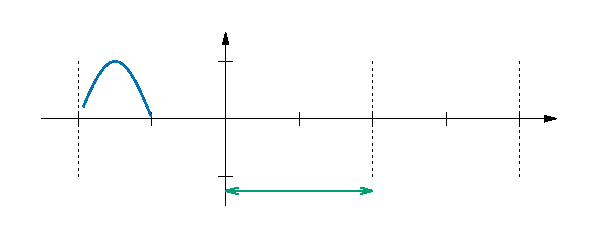
\includegraphics[width={273.60bp},height={100.70bp}]{figura_03_03}}%
    \gplfronttext
  \end{picture}%
\endgroup

\end{figure}

El periodo de la onda rectificada es el mismo que de la onda original.

\subsection{Rectificación de onda completa}

\begin{equation*}
    f(t)=A\,|\sen(\omega_0 t)|
\end{equation*}

\begin{figure}[H]
    \centering
    % GNUPLOT: LaTeX picture with Postscript
\begingroup
  \makeatletter
  \providecommand\color[2][]{%
    \GenericError{(gnuplot) \space\space\space\@spaces}{%
      Package color not loaded in conjunction with
      terminal option `colourtext'%
    }{See the gnuplot documentation for explanation.%
    }{Either use 'blacktext' in gnuplot or load the package
      color.sty in LaTeX.}%
    \renewcommand\color[2][]{}%
  }%
  \providecommand\includegraphics[2][]{%
    \GenericError{(gnuplot) \space\space\space\@spaces}{%
      Package graphicx or graphics not loaded%
    }{See the gnuplot documentation for explanation.%
    }{The gnuplot epslatex terminal needs graphicx.sty or graphics.sty.}%
    \renewcommand\includegraphics[2][]{}%
  }%
  \providecommand\rotatebox[2]{#2}%
  \@ifundefined{ifGPcolor}{%
    \newif\ifGPcolor
    \GPcolorfalse
  }{}%
  \@ifundefined{ifGPblacktext}{%
    \newif\ifGPblacktext
    \GPblacktexttrue
  }{}%
  % define a \g@addto@macro without @ in the name:
  \let\gplgaddtomacro\g@addto@macro
  % define empty templates for all commands taking text:
  \gdef\gplbacktext{}%
  \gdef\gplfronttext{}%
  \makeatother
  \ifGPblacktext
    % no textcolor at all
    \def\colorrgb#1{}%
    \def\colorgray#1{}%
  \else
    % gray or color?
    \ifGPcolor
      \def\colorrgb#1{\color[rgb]{#1}}%
      \def\colorgray#1{\color[gray]{#1}}%
      \expandafter\def\csname LTw\endcsname{\color{white}}%
      \expandafter\def\csname LTb\endcsname{\color{black}}%
      \expandafter\def\csname LTa\endcsname{\color{black}}%
      \expandafter\def\csname LT0\endcsname{\color[rgb]{1,0,0}}%
      \expandafter\def\csname LT1\endcsname{\color[rgb]{0,1,0}}%
      \expandafter\def\csname LT2\endcsname{\color[rgb]{0,0,1}}%
      \expandafter\def\csname LT3\endcsname{\color[rgb]{1,0,1}}%
      \expandafter\def\csname LT4\endcsname{\color[rgb]{0,1,1}}%
      \expandafter\def\csname LT5\endcsname{\color[rgb]{1,1,0}}%
      \expandafter\def\csname LT6\endcsname{\color[rgb]{0,0,0}}%
      \expandafter\def\csname LT7\endcsname{\color[rgb]{1,0.3,0}}%
      \expandafter\def\csname LT8\endcsname{\color[rgb]{0.5,0.5,0.5}}%
    \else
      % gray
      \def\colorrgb#1{\color{black}}%
      \def\colorgray#1{\color[gray]{#1}}%
      \expandafter\def\csname LTw\endcsname{\color{white}}%
      \expandafter\def\csname LTb\endcsname{\color{black}}%
      \expandafter\def\csname LTa\endcsname{\color{black}}%
      \expandafter\def\csname LT0\endcsname{\color{black}}%
      \expandafter\def\csname LT1\endcsname{\color{black}}%
      \expandafter\def\csname LT2\endcsname{\color{black}}%
      \expandafter\def\csname LT3\endcsname{\color{black}}%
      \expandafter\def\csname LT4\endcsname{\color{black}}%
      \expandafter\def\csname LT5\endcsname{\color{black}}%
      \expandafter\def\csname LT6\endcsname{\color{black}}%
      \expandafter\def\csname LT7\endcsname{\color{black}}%
      \expandafter\def\csname LT8\endcsname{\color{black}}%
    \fi
  \fi
    \setlength{\unitlength}{0.0500bp}%
    \ifx\gptboxheight\undefined%
      \newlength{\gptboxheight}%
      \newlength{\gptboxwidth}%
      \newsavebox{\gptboxtext}%
    \fi%
    \setlength{\fboxrule}{0.5pt}%
    \setlength{\fboxsep}{1pt}%
    \definecolor{tbcol}{rgb}{1,1,1}%
\begin{picture}(5472.00,2014.00)%
    \gplgaddtomacro\gplbacktext{%
      \csname LTb\endcsname%%
      \put(1909,469){\makebox(0,0)[r]{\strut{}}}%
      \put(1909,1023){\makebox(0,0)[r]{\strut{}}}%
      \put(1909,1576){\makebox(0,0)[r]{\strut{}}}%
      \put(593,800){\makebox(0,0){\strut{}}}%
      \put(1299,800){\makebox(0,0){\strut{}}}%
      \put(2005,800){\makebox(0,0){\strut{}}}%
      \put(2712,800){\makebox(0,0){\strut{}}}%
      \put(3418,800){\makebox(0,0){\strut{}}}%
      \put(4124,800){\makebox(0,0){\strut{}}}%
      \put(4830,800){\makebox(0,0){\strut{}}}%
      \csname LTb\endcsname%%
      \put(5360,1023){\makebox(0,0)[l]{\strut{}$t$}}%
      \put(2005,1991){\makebox(0,0)[l]{\strut{}$f(t)$}}%
      \put(2330,137){\makebox(0,0)[l]{\strut{}$T$}}%
    }%
    \gplgaddtomacro\gplfronttext{%
    }%
    \gplgaddtomacro\gplbacktext{%
      \csname LTb\endcsname%%
      \put(1909,469){\makebox(0,0)[r]{\strut{}}}%
      \put(1909,1023){\makebox(0,0)[r]{\strut{}}}%
      \put(1909,1576){\makebox(0,0)[r]{\strut{}}}%
      \put(593,800){\makebox(0,0){\strut{}}}%
      \put(1299,800){\makebox(0,0){\strut{}}}%
      \put(2005,800){\makebox(0,0){\strut{}}}%
      \put(2712,800){\makebox(0,0){\strut{}}}%
      \put(3418,800){\makebox(0,0){\strut{}}}%
      \put(4124,800){\makebox(0,0){\strut{}}}%
      \put(4830,800){\makebox(0,0){\strut{}}}%
      \csname LTb\endcsname%%
      \put(5360,1023){\makebox(0,0)[l]{\strut{}$t$}}%
      \put(2005,1991){\makebox(0,0)[l]{\strut{}$f(t)$}}%
      \put(2330,137){\makebox(0,0)[l]{\strut{}$T$}}%
    }%
    \gplgaddtomacro\gplfronttext{%
    }%
    \gplgaddtomacro\gplbacktext{%
      \csname LTb\endcsname%%
      \put(1909,469){\makebox(0,0)[r]{\strut{}}}%
      \put(1909,1023){\makebox(0,0)[r]{\strut{}}}%
      \put(1909,1576){\makebox(0,0)[r]{\strut{}}}%
      \put(593,800){\makebox(0,0){\strut{}}}%
      \put(1299,800){\makebox(0,0){\strut{}}}%
      \put(2005,800){\makebox(0,0){\strut{}}}%
      \put(2712,800){\makebox(0,0){\strut{}}}%
      \put(3418,800){\makebox(0,0){\strut{}}}%
      \put(4124,800){\makebox(0,0){\strut{}}}%
      \put(4830,800){\makebox(0,0){\strut{}}}%
      \csname LTb\endcsname%%
      \put(5360,1023){\makebox(0,0)[l]{\strut{}$t$}}%
      \put(2005,1991){\makebox(0,0)[l]{\strut{}$f(t)$}}%
      \put(2330,137){\makebox(0,0)[l]{\strut{}$T$}}%
    }%
    \gplgaddtomacro\gplfronttext{%
    }%
    \gplgaddtomacro\gplbacktext{%
      \csname LTb\endcsname%%
      \put(1909,469){\makebox(0,0)[r]{\strut{}}}%
      \put(1909,1023){\makebox(0,0)[r]{\strut{}}}%
      \put(1909,1576){\makebox(0,0)[r]{\strut{}}}%
      \put(593,800){\makebox(0,0){\strut{}}}%
      \put(1299,800){\makebox(0,0){\strut{}}}%
      \put(2005,800){\makebox(0,0){\strut{}}}%
      \put(2712,800){\makebox(0,0){\strut{}}}%
      \put(3418,800){\makebox(0,0){\strut{}}}%
      \put(4124,800){\makebox(0,0){\strut{}}}%
      \put(4830,800){\makebox(0,0){\strut{}}}%
      \csname LTb\endcsname%%
      \put(5360,1023){\makebox(0,0)[l]{\strut{}$t$}}%
      \put(2005,1991){\makebox(0,0)[l]{\strut{}$f(t)$}}%
      \put(2330,137){\makebox(0,0)[l]{\strut{}$T$}}%
    }%
    \gplgaddtomacro\gplfronttext{%
    }%
    \gplgaddtomacro\gplbacktext{%
      \csname LTb\endcsname%%
      \put(1909,469){\makebox(0,0)[r]{\strut{}}}%
      \put(1909,1023){\makebox(0,0)[r]{\strut{}}}%
      \put(1909,1576){\makebox(0,0)[r]{\strut{}}}%
      \put(593,800){\makebox(0,0){\strut{}}}%
      \put(1299,800){\makebox(0,0){\strut{}}}%
      \put(2005,800){\makebox(0,0){\strut{}}}%
      \put(2712,800){\makebox(0,0){\strut{}}}%
      \put(3418,800){\makebox(0,0){\strut{}}}%
      \put(4124,800){\makebox(0,0){\strut{}}}%
      \put(4830,800){\makebox(0,0){\strut{}}}%
      \csname LTb\endcsname%%
      \put(5360,1023){\makebox(0,0)[l]{\strut{}$t$}}%
      \put(2005,1991){\makebox(0,0)[l]{\strut{}$f(t)$}}%
      \put(2330,137){\makebox(0,0)[l]{\strut{}$T$}}%
    }%
    \gplgaddtomacro\gplfronttext{%
    }%
    \gplgaddtomacro\gplbacktext{%
      \csname LTb\endcsname%%
      \put(1909,469){\makebox(0,0)[r]{\strut{}}}%
      \put(1909,1023){\makebox(0,0)[r]{\strut{}}}%
      \put(1909,1576){\makebox(0,0)[r]{\strut{}}}%
      \put(593,800){\makebox(0,0){\strut{}}}%
      \put(1299,800){\makebox(0,0){\strut{}}}%
      \put(2005,800){\makebox(0,0){\strut{}}}%
      \put(2712,800){\makebox(0,0){\strut{}}}%
      \put(3418,800){\makebox(0,0){\strut{}}}%
      \put(4124,800){\makebox(0,0){\strut{}}}%
      \put(4830,800){\makebox(0,0){\strut{}}}%
      \csname LTb\endcsname%%
      \put(5360,1023){\makebox(0,0)[l]{\strut{}$t$}}%
      \put(2005,1991){\makebox(0,0)[l]{\strut{}$f(t)$}}%
      \put(2330,137){\makebox(0,0)[l]{\strut{}$T$}}%
    }%
    \gplgaddtomacro\gplfronttext{%
    }%
    \gplgaddtomacro\gplbacktext{%
      \csname LTb\endcsname%%
      \put(1909,469){\makebox(0,0)[r]{\strut{}}}%
      \put(1909,1023){\makebox(0,0)[r]{\strut{}}}%
      \put(1909,1576){\makebox(0,0)[r]{\strut{}}}%
      \put(593,800){\makebox(0,0){\strut{}}}%
      \put(1299,800){\makebox(0,0){\strut{}}}%
      \put(2005,800){\makebox(0,0){\strut{}}}%
      \put(2712,800){\makebox(0,0){\strut{}}}%
      \put(3418,800){\makebox(0,0){\strut{}}}%
      \put(4124,800){\makebox(0,0){\strut{}}}%
      \put(4830,800){\makebox(0,0){\strut{}}}%
      \csname LTb\endcsname%%
      \put(5360,1023){\makebox(0,0)[l]{\strut{}$t$}}%
      \put(2005,1991){\makebox(0,0)[l]{\strut{}$f(t)$}}%
      \put(2330,137){\makebox(0,0)[l]{\strut{}$T$}}%
    }%
    \gplgaddtomacro\gplfronttext{%
    }%
    \gplgaddtomacro\gplbacktext{%
      \csname LTb\endcsname%%
      \put(1909,469){\makebox(0,0)[r]{\strut{}}}%
      \put(1909,1023){\makebox(0,0)[r]{\strut{}}}%
      \put(1909,1576){\makebox(0,0)[r]{\strut{}}}%
      \put(593,800){\makebox(0,0){\strut{}}}%
      \put(1299,800){\makebox(0,0){\strut{}}}%
      \put(2005,800){\makebox(0,0){\strut{}}}%
      \put(2712,800){\makebox(0,0){\strut{}}}%
      \put(3418,800){\makebox(0,0){\strut{}}}%
      \put(4124,800){\makebox(0,0){\strut{}}}%
      \put(4830,800){\makebox(0,0){\strut{}}}%
      \csname LTb\endcsname%%
      \put(5360,1023){\makebox(0,0)[l]{\strut{}$t$}}%
      \put(2005,1991){\makebox(0,0)[l]{\strut{}$f(t)$}}%
      \put(2330,137){\makebox(0,0)[l]{\strut{}$T$}}%
    }%
    \gplgaddtomacro\gplfronttext{%
    }%
    \gplgaddtomacro\gplbacktext{%
      \csname LTb\endcsname%%
      \put(1909,469){\makebox(0,0)[r]{\strut{}}}%
      \put(1909,1023){\makebox(0,0)[r]{\strut{}}}%
      \put(1909,1576){\makebox(0,0)[r]{\strut{}}}%
      \put(593,800){\makebox(0,0){\strut{}}}%
      \put(1299,800){\makebox(0,0){\strut{}}}%
      \put(2005,800){\makebox(0,0){\strut{}}}%
      \put(2712,800){\makebox(0,0){\strut{}}}%
      \put(3418,800){\makebox(0,0){\strut{}}}%
      \put(4124,800){\makebox(0,0){\strut{}}}%
      \put(4830,800){\makebox(0,0){\strut{}}}%
      \csname LTb\endcsname%%
      \put(5360,1023){\makebox(0,0)[l]{\strut{}$t$}}%
      \put(2005,1991){\makebox(0,0)[l]{\strut{}$f(t)$}}%
      \put(2330,137){\makebox(0,0)[l]{\strut{}$T$}}%
    }%
    \gplgaddtomacro\gplfronttext{%
    }%
    \gplbacktext
    \put(0,0){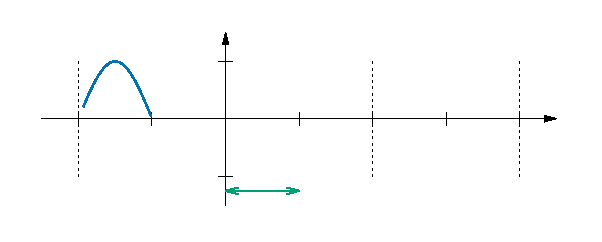
\includegraphics[width={273.60bp},height={100.70bp}]{figura_03_04}}%
    \gplfronttext
  \end{picture}%
\endgroup

\end{figure}

El periodo de la onda rectificada es la mitad del periodo de la onda original.

\section{Función escalón unitario}

\begin{equation*}
    u(t)=\begin{cases}
        0 & t<0\\
        1 & t>0\\
    \end{cases}
\end{equation*}

\begin{figure}[H]
    \centering
    % GNUPLOT: LaTeX picture with Postscript
\begingroup
  \makeatletter
  \providecommand\color[2][]{%
    \GenericError{(gnuplot) \space\space\space\@spaces}{%
      Package color not loaded in conjunction with
      terminal option `colourtext'%
    }{See the gnuplot documentation for explanation.%
    }{Either use 'blacktext' in gnuplot or load the package
      color.sty in LaTeX.}%
    \renewcommand\color[2][]{}%
  }%
  \providecommand\includegraphics[2][]{%
    \GenericError{(gnuplot) \space\space\space\@spaces}{%
      Package graphicx or graphics not loaded%
    }{See the gnuplot documentation for explanation.%
    }{The gnuplot epslatex terminal needs graphicx.sty or graphics.sty.}%
    \renewcommand\includegraphics[2][]{}%
  }%
  \providecommand\rotatebox[2]{#2}%
  \@ifundefined{ifGPcolor}{%
    \newif\ifGPcolor
    \GPcolorfalse
  }{}%
  \@ifundefined{ifGPblacktext}{%
    \newif\ifGPblacktext
    \GPblacktexttrue
  }{}%
  % define a \g@addto@macro without @ in the name:
  \let\gplgaddtomacro\g@addto@macro
  % define empty templates for all commands taking text:
  \gdef\gplbacktext{}%
  \gdef\gplfronttext{}%
  \makeatother
  \ifGPblacktext
    % no textcolor at all
    \def\colorrgb#1{}%
    \def\colorgray#1{}%
  \else
    % gray or color?
    \ifGPcolor
      \def\colorrgb#1{\color[rgb]{#1}}%
      \def\colorgray#1{\color[gray]{#1}}%
      \expandafter\def\csname LTw\endcsname{\color{white}}%
      \expandafter\def\csname LTb\endcsname{\color{black}}%
      \expandafter\def\csname LTa\endcsname{\color{black}}%
      \expandafter\def\csname LT0\endcsname{\color[rgb]{1,0,0}}%
      \expandafter\def\csname LT1\endcsname{\color[rgb]{0,1,0}}%
      \expandafter\def\csname LT2\endcsname{\color[rgb]{0,0,1}}%
      \expandafter\def\csname LT3\endcsname{\color[rgb]{1,0,1}}%
      \expandafter\def\csname LT4\endcsname{\color[rgb]{0,1,1}}%
      \expandafter\def\csname LT5\endcsname{\color[rgb]{1,1,0}}%
      \expandafter\def\csname LT6\endcsname{\color[rgb]{0,0,0}}%
      \expandafter\def\csname LT7\endcsname{\color[rgb]{1,0.3,0}}%
      \expandafter\def\csname LT8\endcsname{\color[rgb]{0.5,0.5,0.5}}%
    \else
      % gray
      \def\colorrgb#1{\color{black}}%
      \def\colorgray#1{\color[gray]{#1}}%
      \expandafter\def\csname LTw\endcsname{\color{white}}%
      \expandafter\def\csname LTb\endcsname{\color{black}}%
      \expandafter\def\csname LTa\endcsname{\color{black}}%
      \expandafter\def\csname LT0\endcsname{\color{black}}%
      \expandafter\def\csname LT1\endcsname{\color{black}}%
      \expandafter\def\csname LT2\endcsname{\color{black}}%
      \expandafter\def\csname LT3\endcsname{\color{black}}%
      \expandafter\def\csname LT4\endcsname{\color{black}}%
      \expandafter\def\csname LT5\endcsname{\color{black}}%
      \expandafter\def\csname LT6\endcsname{\color{black}}%
      \expandafter\def\csname LT7\endcsname{\color{black}}%
      \expandafter\def\csname LT8\endcsname{\color{black}}%
    \fi
  \fi
    \setlength{\unitlength}{0.0500bp}%
    \ifx\gptboxheight\undefined%
      \newlength{\gptboxheight}%
      \newlength{\gptboxwidth}%
      \newsavebox{\gptboxtext}%
    \fi%
    \setlength{\fboxrule}{0.5pt}%
    \setlength{\fboxsep}{1pt}%
    \definecolor{tbcol}{rgb}{1,1,1}%
\begin{picture}(5760.00,1440.00)%
    \gplgaddtomacro\gplbacktext{%
      \csname LTb\endcsname%%
      \put(2760,464){\makebox(0,0)[r]{\strut{}}}%
      \put(2760,1007){\makebox(0,0)[r]{\strut{}}}%
      \put(240,241){\makebox(0,0){\strut{}}}%
      \put(763,241){\makebox(0,0){\strut{}}}%
      \put(1286,241){\makebox(0,0){\strut{}}}%
      \put(1809,241){\makebox(0,0){\strut{}}}%
      \put(2332,241){\makebox(0,0){\strut{}}}%
      \put(2856,241){\makebox(0,0){\strut{}}}%
      \put(3379,241){\makebox(0,0){\strut{}}}%
      \put(3902,241){\makebox(0,0){\strut{}}}%
      \put(4425,241){\makebox(0,0){\strut{}}}%
      \put(4948,241){\makebox(0,0){\strut{}}}%
      \put(5471,241){\makebox(0,0){\strut{}}}%
      \csname LTb\endcsname%%
      \put(6256,464){\makebox(0,0)[l]{\strut{}$t$}}%
      \put(2751,1496){\makebox(0,0)[l]{\strut{}$f(t)$}}%
      \put(2594,1007){\makebox(0,0)[l]{\strut{}$1$}}%
    }%
    \gplgaddtomacro\gplfronttext{%
    }%
    \gplbacktext
    \put(0,0){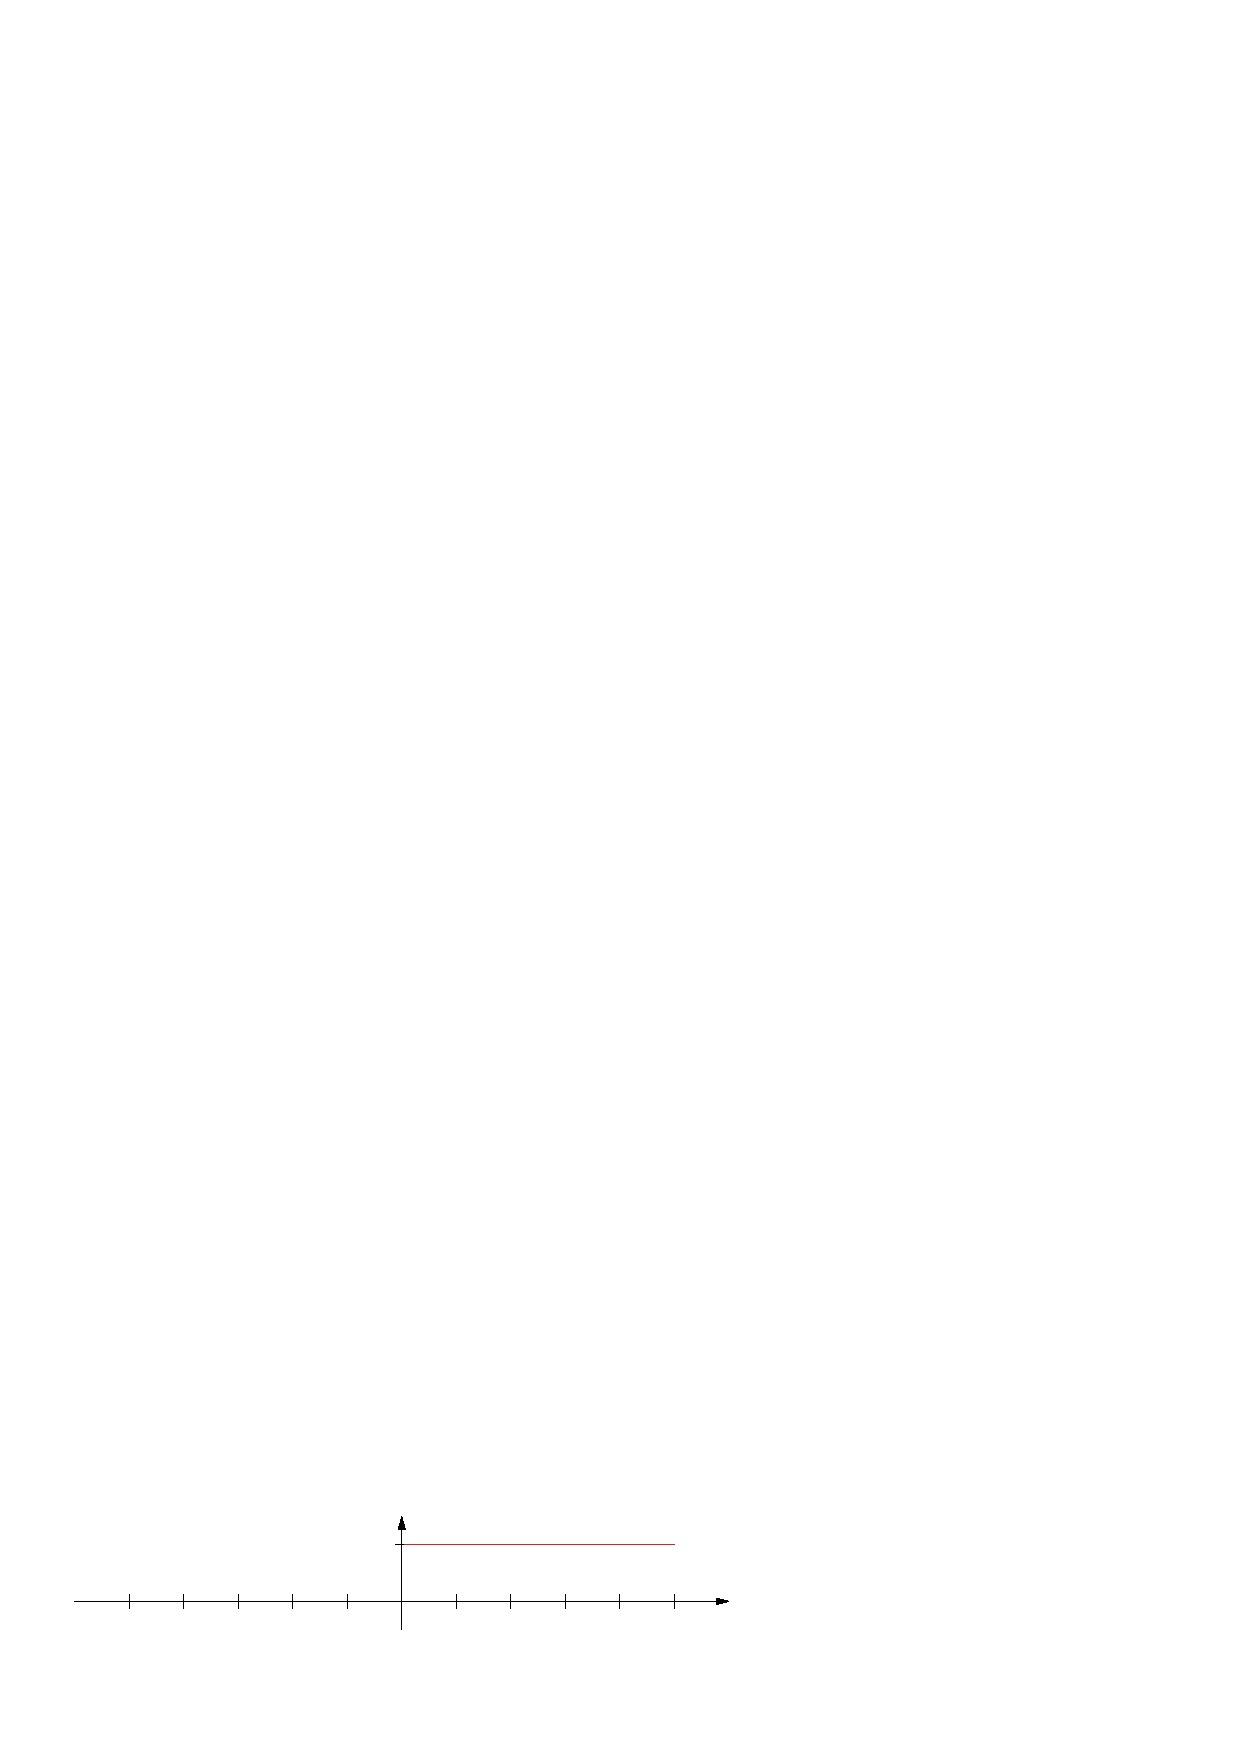
\includegraphics[width={288.00bp},height={72.00bp}]{figura_03_05}}%
    \gplfronttext
  \end{picture}%
\endgroup

\end{figure}

Una variante es:

\begin{equation*}
    u(-t)=\begin{cases}
        1 & t<0\\
        0 & t>0\\
    \end{cases}
\end{equation*}

\begin{figure}[H]
    \centering
    % GNUPLOT: LaTeX picture with Postscript
\begingroup
  \makeatletter
  \providecommand\color[2][]{%
    \GenericError{(gnuplot) \space\space\space\@spaces}{%
      Package color not loaded in conjunction with
      terminal option `colourtext'%
    }{See the gnuplot documentation for explanation.%
    }{Either use 'blacktext' in gnuplot or load the package
      color.sty in LaTeX.}%
    \renewcommand\color[2][]{}%
  }%
  \providecommand\includegraphics[2][]{%
    \GenericError{(gnuplot) \space\space\space\@spaces}{%
      Package graphicx or graphics not loaded%
    }{See the gnuplot documentation for explanation.%
    }{The gnuplot epslatex terminal needs graphicx.sty or graphics.sty.}%
    \renewcommand\includegraphics[2][]{}%
  }%
  \providecommand\rotatebox[2]{#2}%
  \@ifundefined{ifGPcolor}{%
    \newif\ifGPcolor
    \GPcolorfalse
  }{}%
  \@ifundefined{ifGPblacktext}{%
    \newif\ifGPblacktext
    \GPblacktexttrue
  }{}%
  % define a \g@addto@macro without @ in the name:
  \let\gplgaddtomacro\g@addto@macro
  % define empty templates for all commands taking text:
  \gdef\gplbacktext{}%
  \gdef\gplfronttext{}%
  \makeatother
  \ifGPblacktext
    % no textcolor at all
    \def\colorrgb#1{}%
    \def\colorgray#1{}%
  \else
    % gray or color?
    \ifGPcolor
      \def\colorrgb#1{\color[rgb]{#1}}%
      \def\colorgray#1{\color[gray]{#1}}%
      \expandafter\def\csname LTw\endcsname{\color{white}}%
      \expandafter\def\csname LTb\endcsname{\color{black}}%
      \expandafter\def\csname LTa\endcsname{\color{black}}%
      \expandafter\def\csname LT0\endcsname{\color[rgb]{1,0,0}}%
      \expandafter\def\csname LT1\endcsname{\color[rgb]{0,1,0}}%
      \expandafter\def\csname LT2\endcsname{\color[rgb]{0,0,1}}%
      \expandafter\def\csname LT3\endcsname{\color[rgb]{1,0,1}}%
      \expandafter\def\csname LT4\endcsname{\color[rgb]{0,1,1}}%
      \expandafter\def\csname LT5\endcsname{\color[rgb]{1,1,0}}%
      \expandafter\def\csname LT6\endcsname{\color[rgb]{0,0,0}}%
      \expandafter\def\csname LT7\endcsname{\color[rgb]{1,0.3,0}}%
      \expandafter\def\csname LT8\endcsname{\color[rgb]{0.5,0.5,0.5}}%
    \else
      % gray
      \def\colorrgb#1{\color{black}}%
      \def\colorgray#1{\color[gray]{#1}}%
      \expandafter\def\csname LTw\endcsname{\color{white}}%
      \expandafter\def\csname LTb\endcsname{\color{black}}%
      \expandafter\def\csname LTa\endcsname{\color{black}}%
      \expandafter\def\csname LT0\endcsname{\color{black}}%
      \expandafter\def\csname LT1\endcsname{\color{black}}%
      \expandafter\def\csname LT2\endcsname{\color{black}}%
      \expandafter\def\csname LT3\endcsname{\color{black}}%
      \expandafter\def\csname LT4\endcsname{\color{black}}%
      \expandafter\def\csname LT5\endcsname{\color{black}}%
      \expandafter\def\csname LT6\endcsname{\color{black}}%
      \expandafter\def\csname LT7\endcsname{\color{black}}%
      \expandafter\def\csname LT8\endcsname{\color{black}}%
    \fi
  \fi
    \setlength{\unitlength}{0.0500bp}%
    \ifx\gptboxheight\undefined%
      \newlength{\gptboxheight}%
      \newlength{\gptboxwidth}%
      \newsavebox{\gptboxtext}%
    \fi%
    \setlength{\fboxrule}{0.5pt}%
    \setlength{\fboxsep}{1pt}%
    \definecolor{tbcol}{rgb}{1,1,1}%
\begin{picture}(5760.00,1440.00)%
    \gplgaddtomacro\gplbacktext{%
      \csname LTb\endcsname%%
      \put(2760,464){\makebox(0,0)[r]{\strut{}}}%
      \put(2760,1007){\makebox(0,0)[r]{\strut{}}}%
      \put(240,241){\makebox(0,0){\strut{}}}%
      \put(763,241){\makebox(0,0){\strut{}}}%
      \put(1286,241){\makebox(0,0){\strut{}}}%
      \put(1809,241){\makebox(0,0){\strut{}}}%
      \put(2332,241){\makebox(0,0){\strut{}}}%
      \put(2856,241){\makebox(0,0){\strut{}}}%
      \put(3379,241){\makebox(0,0){\strut{}}}%
      \put(3902,241){\makebox(0,0){\strut{}}}%
      \put(4425,241){\makebox(0,0){\strut{}}}%
      \put(4948,241){\makebox(0,0){\strut{}}}%
      \put(5471,241){\makebox(0,0){\strut{}}}%
      \csname LTb\endcsname%%
      \put(6256,464){\makebox(0,0)[l]{\strut{}$t$}}%
      \put(2751,1496){\makebox(0,0)[l]{\strut{}$f(t)$}}%
      \put(3012,1007){\makebox(0,0)[l]{\strut{}$1$}}%
    }%
    \gplgaddtomacro\gplfronttext{%
    }%
    \gplbacktext
    \put(0,0){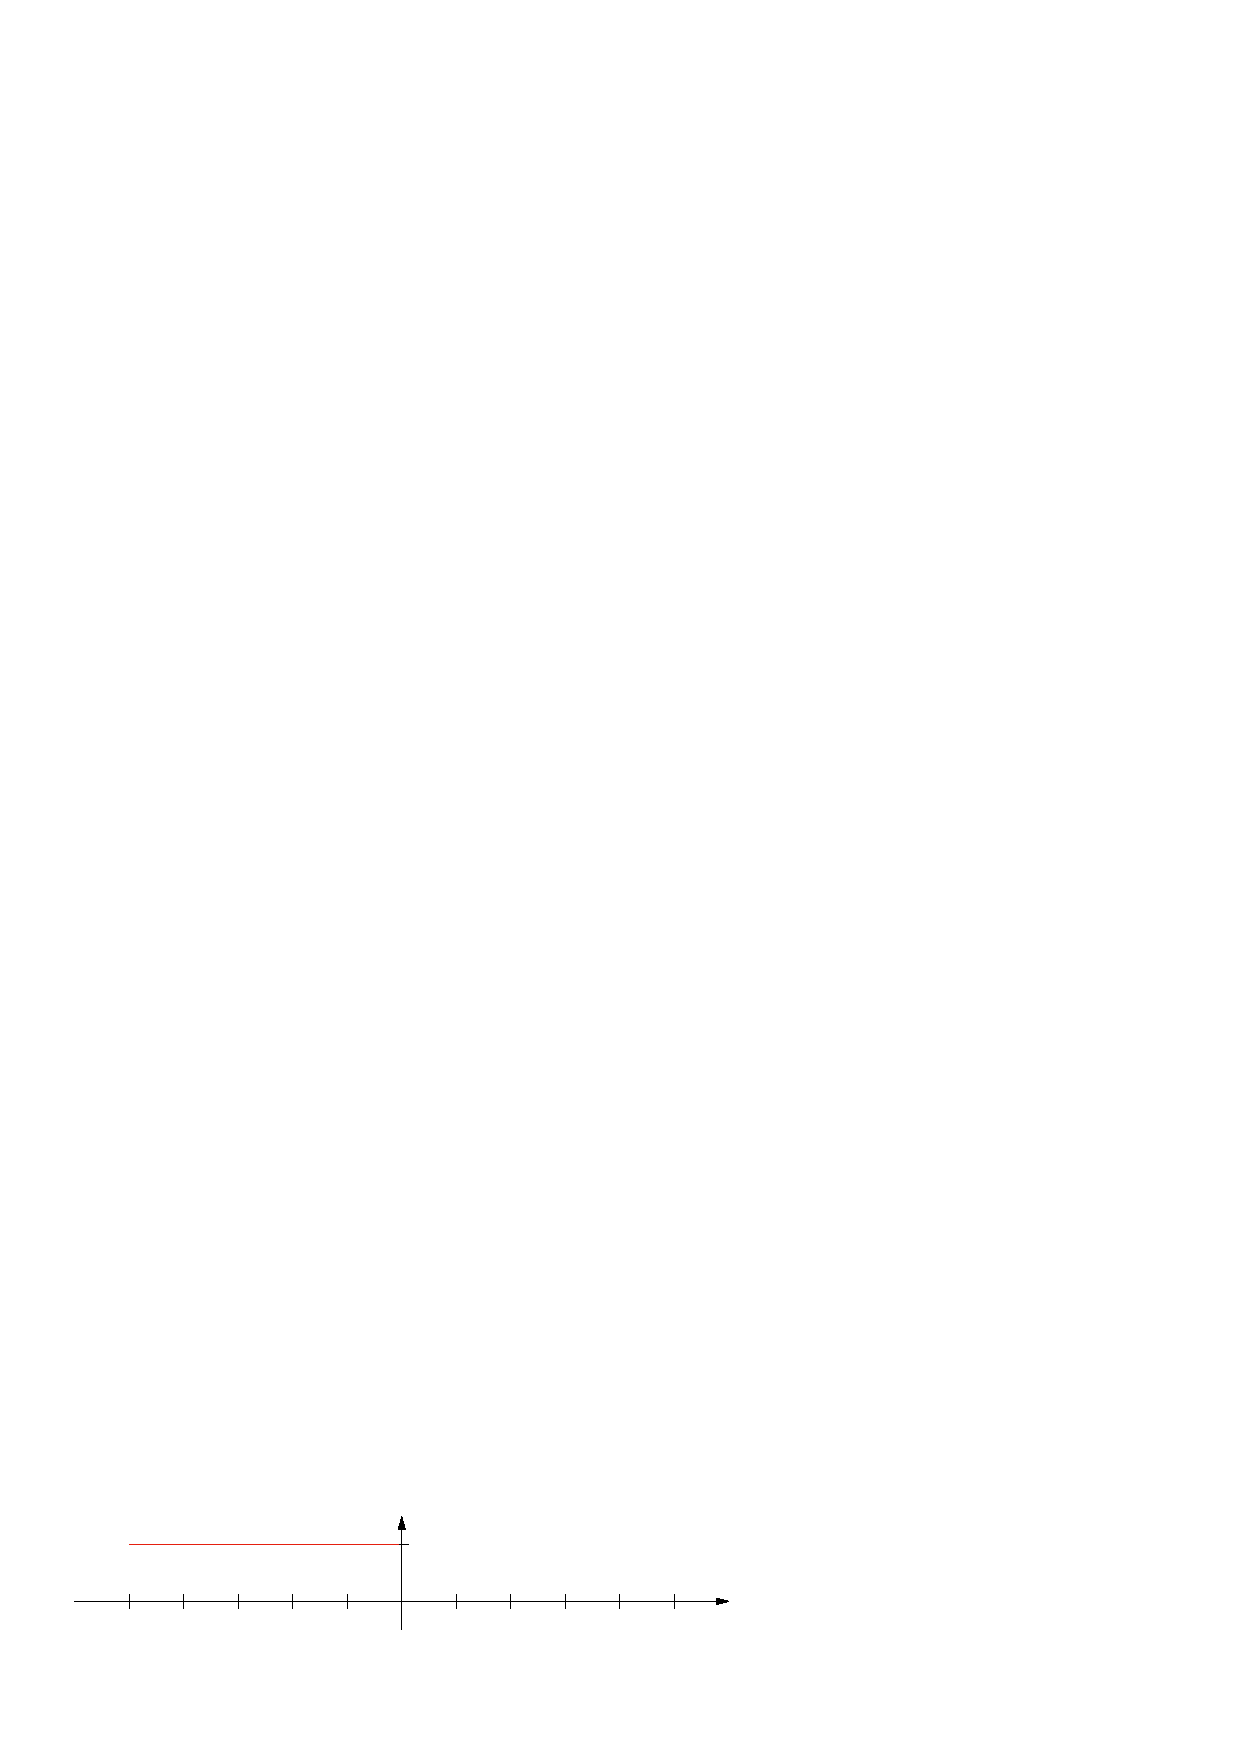
\includegraphics[width={288.00bp},height={72.00bp}]{figura_03_06}}%
    \gplfronttext
  \end{picture}%
\endgroup

\end{figure}

De manera general:

\begin{equation*}
    k\,u(t-t_0)=\begin{cases}
        0 & t<t_0\\
        k & t>t_0\\
    \end{cases}
\end{equation*}

\begin{figure}[H]
    \centering
    % GNUPLOT: LaTeX picture with Postscript
\begingroup
  \makeatletter
  \providecommand\color[2][]{%
    \GenericError{(gnuplot) \space\space\space\@spaces}{%
      Package color not loaded in conjunction with
      terminal option `colourtext'%
    }{See the gnuplot documentation for explanation.%
    }{Either use 'blacktext' in gnuplot or load the package
      color.sty in LaTeX.}%
    \renewcommand\color[2][]{}%
  }%
  \providecommand\includegraphics[2][]{%
    \GenericError{(gnuplot) \space\space\space\@spaces}{%
      Package graphicx or graphics not loaded%
    }{See the gnuplot documentation for explanation.%
    }{The gnuplot epslatex terminal needs graphicx.sty or graphics.sty.}%
    \renewcommand\includegraphics[2][]{}%
  }%
  \providecommand\rotatebox[2]{#2}%
  \@ifundefined{ifGPcolor}{%
    \newif\ifGPcolor
    \GPcolorfalse
  }{}%
  \@ifundefined{ifGPblacktext}{%
    \newif\ifGPblacktext
    \GPblacktexttrue
  }{}%
  % define a \g@addto@macro without @ in the name:
  \let\gplgaddtomacro\g@addto@macro
  % define empty templates for all commands taking text:
  \gdef\gplbacktext{}%
  \gdef\gplfronttext{}%
  \makeatother
  \ifGPblacktext
    % no textcolor at all
    \def\colorrgb#1{}%
    \def\colorgray#1{}%
  \else
    % gray or color?
    \ifGPcolor
      \def\colorrgb#1{\color[rgb]{#1}}%
      \def\colorgray#1{\color[gray]{#1}}%
      \expandafter\def\csname LTw\endcsname{\color{white}}%
      \expandafter\def\csname LTb\endcsname{\color{black}}%
      \expandafter\def\csname LTa\endcsname{\color{black}}%
      \expandafter\def\csname LT0\endcsname{\color[rgb]{1,0,0}}%
      \expandafter\def\csname LT1\endcsname{\color[rgb]{0,1,0}}%
      \expandafter\def\csname LT2\endcsname{\color[rgb]{0,0,1}}%
      \expandafter\def\csname LT3\endcsname{\color[rgb]{1,0,1}}%
      \expandafter\def\csname LT4\endcsname{\color[rgb]{0,1,1}}%
      \expandafter\def\csname LT5\endcsname{\color[rgb]{1,1,0}}%
      \expandafter\def\csname LT6\endcsname{\color[rgb]{0,0,0}}%
      \expandafter\def\csname LT7\endcsname{\color[rgb]{1,0.3,0}}%
      \expandafter\def\csname LT8\endcsname{\color[rgb]{0.5,0.5,0.5}}%
    \else
      % gray
      \def\colorrgb#1{\color{black}}%
      \def\colorgray#1{\color[gray]{#1}}%
      \expandafter\def\csname LTw\endcsname{\color{white}}%
      \expandafter\def\csname LTb\endcsname{\color{black}}%
      \expandafter\def\csname LTa\endcsname{\color{black}}%
      \expandafter\def\csname LT0\endcsname{\color{black}}%
      \expandafter\def\csname LT1\endcsname{\color{black}}%
      \expandafter\def\csname LT2\endcsname{\color{black}}%
      \expandafter\def\csname LT3\endcsname{\color{black}}%
      \expandafter\def\csname LT4\endcsname{\color{black}}%
      \expandafter\def\csname LT5\endcsname{\color{black}}%
      \expandafter\def\csname LT6\endcsname{\color{black}}%
      \expandafter\def\csname LT7\endcsname{\color{black}}%
      \expandafter\def\csname LT8\endcsname{\color{black}}%
    \fi
  \fi
    \setlength{\unitlength}{0.0500bp}%
    \ifx\gptboxheight\undefined%
      \newlength{\gptboxheight}%
      \newlength{\gptboxwidth}%
      \newsavebox{\gptboxtext}%
    \fi%
    \setlength{\fboxrule}{0.5pt}%
    \setlength{\fboxsep}{1pt}%
    \definecolor{tbcol}{rgb}{1,1,1}%
\begin{picture}(5760.00,2160.00)%
    \gplgaddtomacro\gplbacktext{%
      \csname LTb\endcsname%%
      \put(2760,493){\makebox(0,0)[r]{\strut{}}}%
      \put(2760,1096){\makebox(0,0)[r]{\strut{}}}%
      \put(2760,1698){\makebox(0,0)[r]{\strut{}}}%
      \put(240,270){\makebox(0,0){\strut{}}}%
      \put(763,270){\makebox(0,0){\strut{}}}%
      \put(1286,270){\makebox(0,0){\strut{}}}%
      \put(1809,270){\makebox(0,0){\strut{}}}%
      \put(2332,270){\makebox(0,0){\strut{}}}%
      \put(2856,270){\makebox(0,0){\strut{}}}%
      \put(3379,270){\makebox(0,0){\strut{}}}%
      \put(3902,270){\makebox(0,0){\strut{}}}%
      \put(4425,270){\makebox(0,0){\strut{}}}%
      \put(4948,270){\makebox(0,0){\strut{}}}%
      \put(5471,270){\makebox(0,0){\strut{}}}%
      \csname LTb\endcsname%%
      \put(6256,493){\makebox(0,0)[l]{\strut{}$t$}}%
      \put(2751,2240){\makebox(0,0)[l]{\strut{}$f(t)$}}%
      \put(3588,312){\makebox(0,0)[l]{\strut{}$t_0$}}%
      \put(2594,1397){\makebox(0,0)[l]{\strut{}$k$}}%
    }%
    \gplgaddtomacro\gplfronttext{%
    }%
    \gplbacktext
    \put(0,0){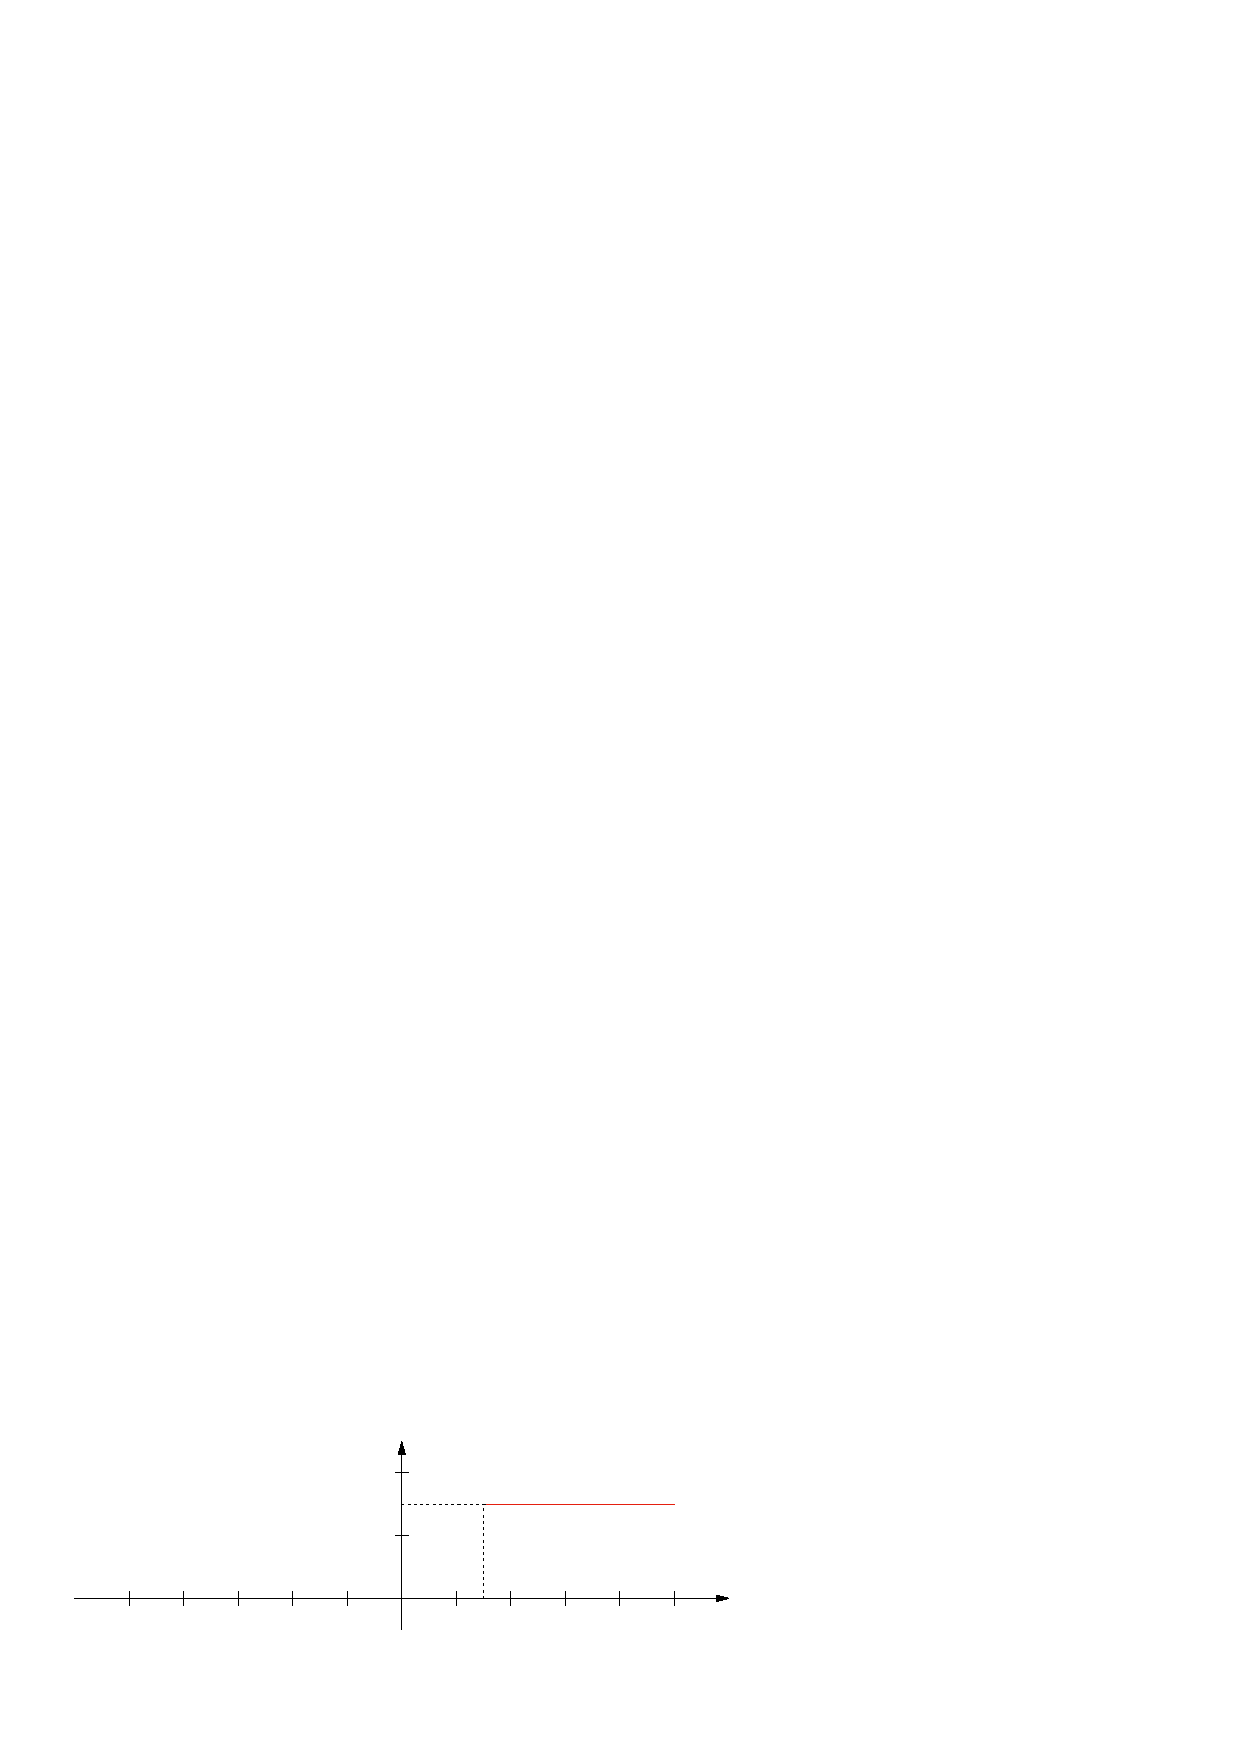
\includegraphics[width={288.00bp},height={108.00bp}]{figura_03_07}}%
    \gplfronttext
  \end{picture}%
\endgroup

\end{figure}

Si: $\phi(t)$ es una función de prueba:

\begin{figure}[H]
    \centering
    % GNUPLOT: LaTeX picture with Postscript
\begingroup
  \makeatletter
  \providecommand\color[2][]{%
    \GenericError{(gnuplot) \space\space\space\@spaces}{%
      Package color not loaded in conjunction with
      terminal option `colourtext'%
    }{See the gnuplot documentation for explanation.%
    }{Either use 'blacktext' in gnuplot or load the package
      color.sty in LaTeX.}%
    \renewcommand\color[2][]{}%
  }%
  \providecommand\includegraphics[2][]{%
    \GenericError{(gnuplot) \space\space\space\@spaces}{%
      Package graphicx or graphics not loaded%
    }{See the gnuplot documentation for explanation.%
    }{The gnuplot epslatex terminal needs graphicx.sty or graphics.sty.}%
    \renewcommand\includegraphics[2][]{}%
  }%
  \providecommand\rotatebox[2]{#2}%
  \@ifundefined{ifGPcolor}{%
    \newif\ifGPcolor
    \GPcolorfalse
  }{}%
  \@ifundefined{ifGPblacktext}{%
    \newif\ifGPblacktext
    \GPblacktexttrue
  }{}%
  % define a \g@addto@macro without @ in the name:
  \let\gplgaddtomacro\g@addto@macro
  % define empty templates for all commands taking text:
  \gdef\gplbacktext{}%
  \gdef\gplfronttext{}%
  \makeatother
  \ifGPblacktext
    % no textcolor at all
    \def\colorrgb#1{}%
    \def\colorgray#1{}%
  \else
    % gray or color?
    \ifGPcolor
      \def\colorrgb#1{\color[rgb]{#1}}%
      \def\colorgray#1{\color[gray]{#1}}%
      \expandafter\def\csname LTw\endcsname{\color{white}}%
      \expandafter\def\csname LTb\endcsname{\color{black}}%
      \expandafter\def\csname LTa\endcsname{\color{black}}%
      \expandafter\def\csname LT0\endcsname{\color[rgb]{1,0,0}}%
      \expandafter\def\csname LT1\endcsname{\color[rgb]{0,1,0}}%
      \expandafter\def\csname LT2\endcsname{\color[rgb]{0,0,1}}%
      \expandafter\def\csname LT3\endcsname{\color[rgb]{1,0,1}}%
      \expandafter\def\csname LT4\endcsname{\color[rgb]{0,1,1}}%
      \expandafter\def\csname LT5\endcsname{\color[rgb]{1,1,0}}%
      \expandafter\def\csname LT6\endcsname{\color[rgb]{0,0,0}}%
      \expandafter\def\csname LT7\endcsname{\color[rgb]{1,0.3,0}}%
      \expandafter\def\csname LT8\endcsname{\color[rgb]{0.5,0.5,0.5}}%
    \else
      % gray
      \def\colorrgb#1{\color{black}}%
      \def\colorgray#1{\color[gray]{#1}}%
      \expandafter\def\csname LTw\endcsname{\color{white}}%
      \expandafter\def\csname LTb\endcsname{\color{black}}%
      \expandafter\def\csname LTa\endcsname{\color{black}}%
      \expandafter\def\csname LT0\endcsname{\color{black}}%
      \expandafter\def\csname LT1\endcsname{\color{black}}%
      \expandafter\def\csname LT2\endcsname{\color{black}}%
      \expandafter\def\csname LT3\endcsname{\color{black}}%
      \expandafter\def\csname LT4\endcsname{\color{black}}%
      \expandafter\def\csname LT5\endcsname{\color{black}}%
      \expandafter\def\csname LT6\endcsname{\color{black}}%
      \expandafter\def\csname LT7\endcsname{\color{black}}%
      \expandafter\def\csname LT8\endcsname{\color{black}}%
    \fi
  \fi
    \setlength{\unitlength}{0.0500bp}%
    \ifx\gptboxheight\undefined%
      \newlength{\gptboxheight}%
      \newlength{\gptboxwidth}%
      \newsavebox{\gptboxtext}%
    \fi%
    \setlength{\fboxrule}{0.5pt}%
    \setlength{\fboxsep}{1pt}%
    \definecolor{tbcol}{rgb}{1,1,1}%
\begin{picture}(4320.00,2880.00)%
    \gplgaddtomacro\gplbacktext{%
      \csname LTb\endcsname%%
      \put(2040,192){\makebox(0,0)[r]{\strut{}}}%
      \put(2040,553){\makebox(0,0)[r]{\strut{}}}%
      \put(2040,914){\makebox(0,0)[r]{\strut{}}}%
      \put(2040,1275){\makebox(0,0)[r]{\strut{}}}%
      \put(2040,1636){\makebox(0,0)[r]{\strut{}}}%
      \put(2040,1997){\makebox(0,0)[r]{\strut{}}}%
      \put(2040,2358){\makebox(0,0)[r]{\strut{}}}%
      \put(2040,2719){\makebox(0,0)[r]{\strut{}}}%
      \put(240,330){\makebox(0,0){\strut{}}}%
      \put(714,330){\makebox(0,0){\strut{}}}%
      \put(1188,330){\makebox(0,0){\strut{}}}%
      \put(1662,330){\makebox(0,0){\strut{}}}%
      \put(2136,330){\makebox(0,0){\strut{}}}%
      \put(2609,330){\makebox(0,0){\strut{}}}%
      \put(3083,330){\makebox(0,0){\strut{}}}%
      \put(3557,330){\makebox(0,0){\strut{}}}%
      \put(4031,330){\makebox(0,0){\strut{}}}%
      \csname LTb\endcsname%%
      \put(4647,553){\makebox(0,0)[l]{\strut{}$t$}}%
      \put(2349,2863){\makebox(0,0)[l]{\strut{}$f(t)$}}%
      \put(2562,336){\makebox(0,0)[l]{\strut{}$t_0$}}%
      \put(1851,914){\makebox(0,0)[l]{\strut{}$1$}}%
      \put(714,2178){\makebox(0,0)[l]{\strut{}$\phi(t)$}}%
      \put(3083,1095){\makebox(0,0)[l]{\strut{}$u(t-t_0)$}}%
    }%
    \gplgaddtomacro\gplfronttext{%
    }%
    \gplgaddtomacro\gplbacktext{%
      \csname LTb\endcsname%%
      \put(2040,192){\makebox(0,0)[r]{\strut{}}}%
      \put(2040,553){\makebox(0,0)[r]{\strut{}}}%
      \put(2040,914){\makebox(0,0)[r]{\strut{}}}%
      \put(2040,1275){\makebox(0,0)[r]{\strut{}}}%
      \put(2040,1636){\makebox(0,0)[r]{\strut{}}}%
      \put(2040,1997){\makebox(0,0)[r]{\strut{}}}%
      \put(2040,2358){\makebox(0,0)[r]{\strut{}}}%
      \put(2040,2719){\makebox(0,0)[r]{\strut{}}}%
      \put(240,330){\makebox(0,0){\strut{}}}%
      \put(714,330){\makebox(0,0){\strut{}}}%
      \put(1188,330){\makebox(0,0){\strut{}}}%
      \put(1662,330){\makebox(0,0){\strut{}}}%
      \put(2136,330){\makebox(0,0){\strut{}}}%
      \put(2609,330){\makebox(0,0){\strut{}}}%
      \put(3083,330){\makebox(0,0){\strut{}}}%
      \put(3557,330){\makebox(0,0){\strut{}}}%
      \put(4031,330){\makebox(0,0){\strut{}}}%
      \csname LTb\endcsname%%
      \put(4647,553){\makebox(0,0)[l]{\strut{}$t$}}%
      \put(2349,2863){\makebox(0,0)[l]{\strut{}$f(t)$}}%
      \put(2562,336){\makebox(0,0)[l]{\strut{}$t_0$}}%
      \put(1851,914){\makebox(0,0)[l]{\strut{}$1$}}%
      \put(714,2178){\makebox(0,0)[l]{\strut{}$\phi(t)$}}%
      \put(3083,1095){\makebox(0,0)[l]{\strut{}$u(t-t_0)$}}%
    }%
    \gplgaddtomacro\gplfronttext{%
    }%
    \gplbacktext
    \put(0,0){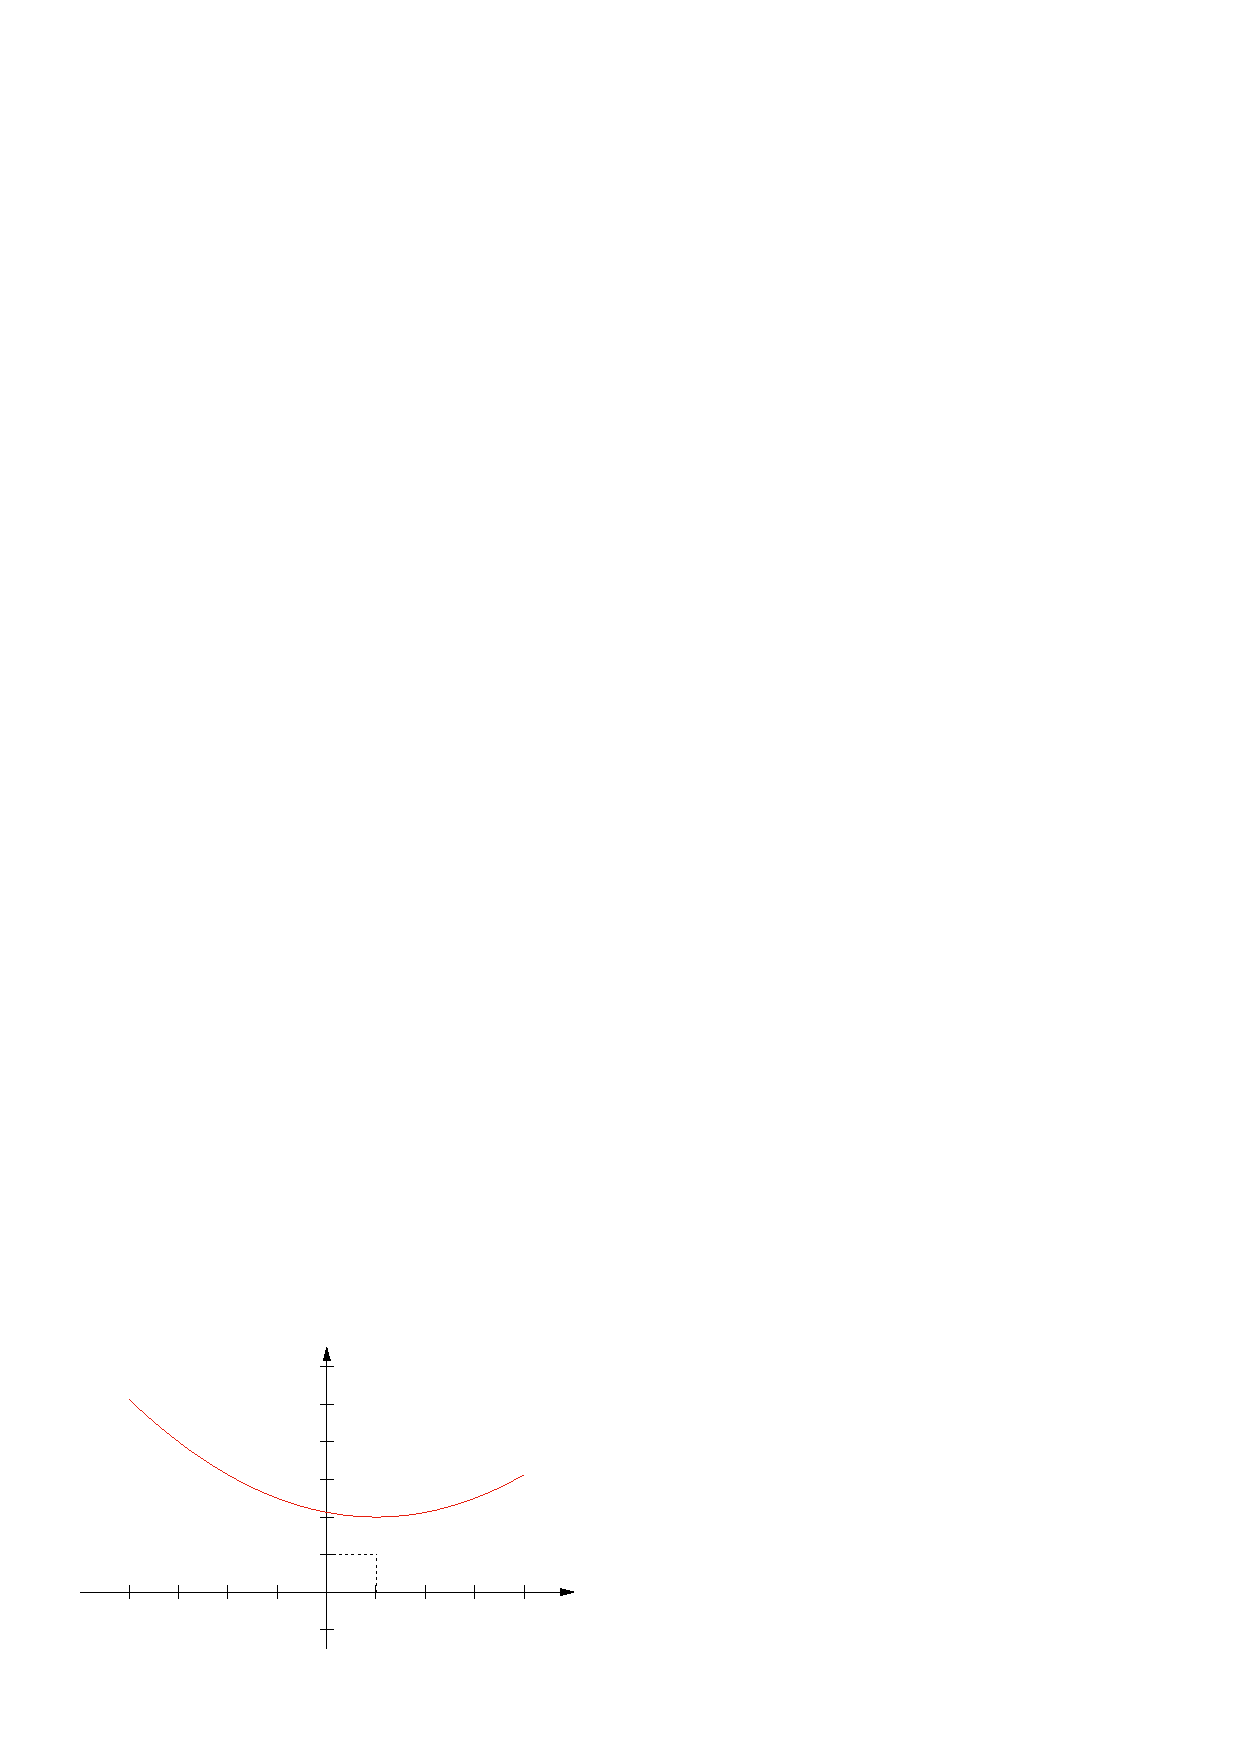
\includegraphics[width={216.00bp},height={144.00bp}]{figura_03_08}}%
    \gplfronttext
  \end{picture}%
\endgroup

\end{figure}

\begin{equation*}
    \phi(t)u(t-t_0)=\begin{cases}
        0       & t<t_0\\
        \phi(t) & t>t_0\\
    \end{cases}
\end{equation*}

\begin{figure}[H]
    \centering
    % GNUPLOT: LaTeX picture with Postscript
\begingroup
  \makeatletter
  \providecommand\color[2][]{%
    \GenericError{(gnuplot) \space\space\space\@spaces}{%
      Package color not loaded in conjunction with
      terminal option `colourtext'%
    }{See the gnuplot documentation for explanation.%
    }{Either use 'blacktext' in gnuplot or load the package
      color.sty in LaTeX.}%
    \renewcommand\color[2][]{}%
  }%
  \providecommand\includegraphics[2][]{%
    \GenericError{(gnuplot) \space\space\space\@spaces}{%
      Package graphicx or graphics not loaded%
    }{See the gnuplot documentation for explanation.%
    }{The gnuplot epslatex terminal needs graphicx.sty or graphics.sty.}%
    \renewcommand\includegraphics[2][]{}%
  }%
  \providecommand\rotatebox[2]{#2}%
  \@ifundefined{ifGPcolor}{%
    \newif\ifGPcolor
    \GPcolorfalse
  }{}%
  \@ifundefined{ifGPblacktext}{%
    \newif\ifGPblacktext
    \GPblacktexttrue
  }{}%
  % define a \g@addto@macro without @ in the name:
  \let\gplgaddtomacro\g@addto@macro
  % define empty templates for all commands taking text:
  \gdef\gplbacktext{}%
  \gdef\gplfronttext{}%
  \makeatother
  \ifGPblacktext
    % no textcolor at all
    \def\colorrgb#1{}%
    \def\colorgray#1{}%
  \else
    % gray or color?
    \ifGPcolor
      \def\colorrgb#1{\color[rgb]{#1}}%
      \def\colorgray#1{\color[gray]{#1}}%
      \expandafter\def\csname LTw\endcsname{\color{white}}%
      \expandafter\def\csname LTb\endcsname{\color{black}}%
      \expandafter\def\csname LTa\endcsname{\color{black}}%
      \expandafter\def\csname LT0\endcsname{\color[rgb]{1,0,0}}%
      \expandafter\def\csname LT1\endcsname{\color[rgb]{0,1,0}}%
      \expandafter\def\csname LT2\endcsname{\color[rgb]{0,0,1}}%
      \expandafter\def\csname LT3\endcsname{\color[rgb]{1,0,1}}%
      \expandafter\def\csname LT4\endcsname{\color[rgb]{0,1,1}}%
      \expandafter\def\csname LT5\endcsname{\color[rgb]{1,1,0}}%
      \expandafter\def\csname LT6\endcsname{\color[rgb]{0,0,0}}%
      \expandafter\def\csname LT7\endcsname{\color[rgb]{1,0.3,0}}%
      \expandafter\def\csname LT8\endcsname{\color[rgb]{0.5,0.5,0.5}}%
    \else
      % gray
      \def\colorrgb#1{\color{black}}%
      \def\colorgray#1{\color[gray]{#1}}%
      \expandafter\def\csname LTw\endcsname{\color{white}}%
      \expandafter\def\csname LTb\endcsname{\color{black}}%
      \expandafter\def\csname LTa\endcsname{\color{black}}%
      \expandafter\def\csname LT0\endcsname{\color{black}}%
      \expandafter\def\csname LT1\endcsname{\color{black}}%
      \expandafter\def\csname LT2\endcsname{\color{black}}%
      \expandafter\def\csname LT3\endcsname{\color{black}}%
      \expandafter\def\csname LT4\endcsname{\color{black}}%
      \expandafter\def\csname LT5\endcsname{\color{black}}%
      \expandafter\def\csname LT6\endcsname{\color{black}}%
      \expandafter\def\csname LT7\endcsname{\color{black}}%
      \expandafter\def\csname LT8\endcsname{\color{black}}%
    \fi
  \fi
    \setlength{\unitlength}{0.0500bp}%
    \ifx\gptboxheight\undefined%
      \newlength{\gptboxheight}%
      \newlength{\gptboxwidth}%
      \newsavebox{\gptboxtext}%
    \fi%
    \setlength{\fboxrule}{0.5pt}%
    \setlength{\fboxsep}{1pt}%
    \definecolor{tbcol}{rgb}{1,1,1}%
\begin{picture}(4320.00,2880.00)%
    \gplgaddtomacro\gplbacktext{%
      \csname LTb\endcsname%%
      \put(2040,192){\makebox(0,0)[r]{\strut{}}}%
      \put(2040,553){\makebox(0,0)[r]{\strut{}}}%
      \put(2040,914){\makebox(0,0)[r]{\strut{}}}%
      \put(2040,1275){\makebox(0,0)[r]{\strut{}}}%
      \put(2040,1636){\makebox(0,0)[r]{\strut{}}}%
      \put(2040,1997){\makebox(0,0)[r]{\strut{}}}%
      \put(2040,2358){\makebox(0,0)[r]{\strut{}}}%
      \put(2040,2719){\makebox(0,0)[r]{\strut{}}}%
      \put(240,330){\makebox(0,0){\strut{}}}%
      \put(714,330){\makebox(0,0){\strut{}}}%
      \put(1188,330){\makebox(0,0){\strut{}}}%
      \put(1662,330){\makebox(0,0){\strut{}}}%
      \put(2136,330){\makebox(0,0){\strut{}}}%
      \put(2609,330){\makebox(0,0){\strut{}}}%
      \put(3083,330){\makebox(0,0){\strut{}}}%
      \put(3557,330){\makebox(0,0){\strut{}}}%
      \put(4031,330){\makebox(0,0){\strut{}}}%
      \csname LTb\endcsname%%
      \put(4647,553){\makebox(0,0)[l]{\strut{}$t$}}%
      \put(2349,2863){\makebox(0,0)[l]{\strut{}$f(t)$}}%
      \put(2562,336){\makebox(0,0)[l]{\strut{}$t_0$}}%
      \put(3083,1095){\makebox(0,0)[l]{\strut{}$\phi(t)u(t-t_0)$}}%
    }%
    \gplgaddtomacro\gplfronttext{%
    }%
    \gplbacktext
    \put(0,0){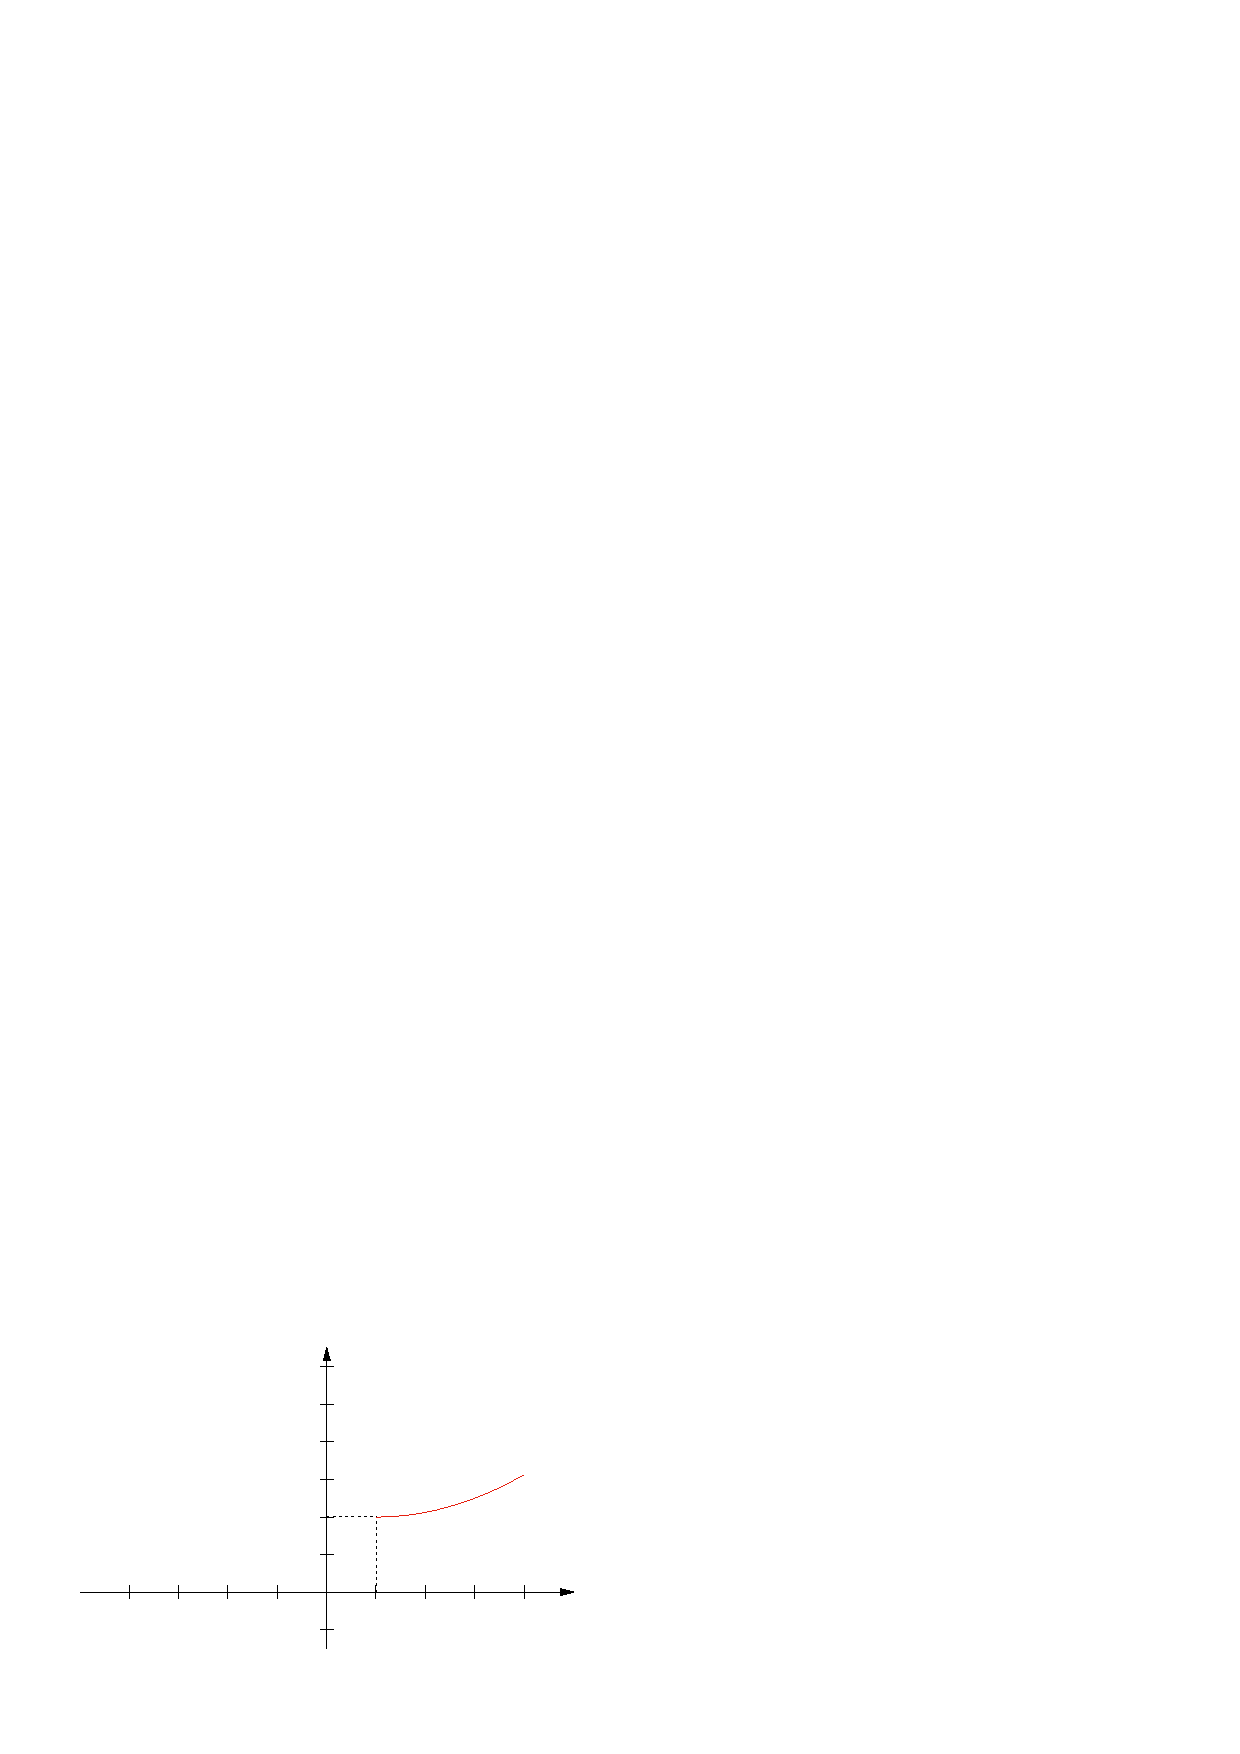
\includegraphics[width={216.00bp},height={144.00bp}]{figura_03_09}}%
    \gplfronttext
  \end{picture}%
\endgroup

\end{figure}

\begin{equation*}
    \phi(t)(u(t-t_1)-u(t-t_2))=\begin{cases}
        0       & t\notin[t_1,t_2]\\
        \phi(t) & t\in[t_1,t_2]\\
    \end{cases}
\end{equation*}

\begin{figure}[H]
    \centering
    % GNUPLOT: LaTeX picture with Postscript
\begingroup
  \makeatletter
  \providecommand\color[2][]{%
    \GenericError{(gnuplot) \space\space\space\@spaces}{%
      Package color not loaded in conjunction with
      terminal option `colourtext'%
    }{See the gnuplot documentation for explanation.%
    }{Either use 'blacktext' in gnuplot or load the package
      color.sty in LaTeX.}%
    \renewcommand\color[2][]{}%
  }%
  \providecommand\includegraphics[2][]{%
    \GenericError{(gnuplot) \space\space\space\@spaces}{%
      Package graphicx or graphics not loaded%
    }{See the gnuplot documentation for explanation.%
    }{The gnuplot epslatex terminal needs graphicx.sty or graphics.sty.}%
    \renewcommand\includegraphics[2][]{}%
  }%
  \providecommand\rotatebox[2]{#2}%
  \@ifundefined{ifGPcolor}{%
    \newif\ifGPcolor
    \GPcolorfalse
  }{}%
  \@ifundefined{ifGPblacktext}{%
    \newif\ifGPblacktext
    \GPblacktexttrue
  }{}%
  % define a \g@addto@macro without @ in the name:
  \let\gplgaddtomacro\g@addto@macro
  % define empty templates for all commands taking text:
  \gdef\gplbacktext{}%
  \gdef\gplfronttext{}%
  \makeatother
  \ifGPblacktext
    % no textcolor at all
    \def\colorrgb#1{}%
    \def\colorgray#1{}%
  \else
    % gray or color?
    \ifGPcolor
      \def\colorrgb#1{\color[rgb]{#1}}%
      \def\colorgray#1{\color[gray]{#1}}%
      \expandafter\def\csname LTw\endcsname{\color{white}}%
      \expandafter\def\csname LTb\endcsname{\color{black}}%
      \expandafter\def\csname LTa\endcsname{\color{black}}%
      \expandafter\def\csname LT0\endcsname{\color[rgb]{1,0,0}}%
      \expandafter\def\csname LT1\endcsname{\color[rgb]{0,1,0}}%
      \expandafter\def\csname LT2\endcsname{\color[rgb]{0,0,1}}%
      \expandafter\def\csname LT3\endcsname{\color[rgb]{1,0,1}}%
      \expandafter\def\csname LT4\endcsname{\color[rgb]{0,1,1}}%
      \expandafter\def\csname LT5\endcsname{\color[rgb]{1,1,0}}%
      \expandafter\def\csname LT6\endcsname{\color[rgb]{0,0,0}}%
      \expandafter\def\csname LT7\endcsname{\color[rgb]{1,0.3,0}}%
      \expandafter\def\csname LT8\endcsname{\color[rgb]{0.5,0.5,0.5}}%
    \else
      % gray
      \def\colorrgb#1{\color{black}}%
      \def\colorgray#1{\color[gray]{#1}}%
      \expandafter\def\csname LTw\endcsname{\color{white}}%
      \expandafter\def\csname LTb\endcsname{\color{black}}%
      \expandafter\def\csname LTa\endcsname{\color{black}}%
      \expandafter\def\csname LT0\endcsname{\color{black}}%
      \expandafter\def\csname LT1\endcsname{\color{black}}%
      \expandafter\def\csname LT2\endcsname{\color{black}}%
      \expandafter\def\csname LT3\endcsname{\color{black}}%
      \expandafter\def\csname LT4\endcsname{\color{black}}%
      \expandafter\def\csname LT5\endcsname{\color{black}}%
      \expandafter\def\csname LT6\endcsname{\color{black}}%
      \expandafter\def\csname LT7\endcsname{\color{black}}%
      \expandafter\def\csname LT8\endcsname{\color{black}}%
    \fi
  \fi
    \setlength{\unitlength}{0.0500bp}%
    \ifx\gptboxheight\undefined%
      \newlength{\gptboxheight}%
      \newlength{\gptboxwidth}%
      \newsavebox{\gptboxtext}%
    \fi%
    \setlength{\fboxrule}{0.5pt}%
    \setlength{\fboxsep}{1pt}%
    \definecolor{tbcol}{rgb}{1,1,1}%
\begin{picture}(4320.00,2880.00)%
    \gplgaddtomacro\gplbacktext{%
      \csname LTb\endcsname%%
      \put(2040,192){\makebox(0,0)[r]{\strut{}}}%
      \put(2040,553){\makebox(0,0)[r]{\strut{}}}%
      \put(2040,914){\makebox(0,0)[r]{\strut{}}}%
      \put(2040,1275){\makebox(0,0)[r]{\strut{}}}%
      \put(2040,1636){\makebox(0,0)[r]{\strut{}}}%
      \put(2040,1997){\makebox(0,0)[r]{\strut{}}}%
      \put(2040,2358){\makebox(0,0)[r]{\strut{}}}%
      \put(2040,2719){\makebox(0,0)[r]{\strut{}}}%
      \put(240,330){\makebox(0,0){\strut{}}}%
      \put(714,330){\makebox(0,0){\strut{}}}%
      \put(1188,330){\makebox(0,0){\strut{}}}%
      \put(1662,330){\makebox(0,0){\strut{}}}%
      \put(2136,330){\makebox(0,0){\strut{}}}%
      \put(2609,330){\makebox(0,0){\strut{}}}%
      \put(3083,330){\makebox(0,0){\strut{}}}%
      \put(3557,330){\makebox(0,0){\strut{}}}%
      \put(4031,330){\makebox(0,0){\strut{}}}%
      \csname LTb\endcsname%%
      \put(4647,553){\makebox(0,0)[l]{\strut{}$t$}}%
      \put(2349,2863){\makebox(0,0)[l]{\strut{}$f(t)$}}%
      \put(2562,336){\makebox(0,0)[l]{\strut{}$t_1$}}%
      \put(3510,336){\makebox(0,0)[l]{\strut{}$t_2$}}%
      \put(2609,1817){\makebox(0,0)[l]{\strut{}$\phi(t)(u(t-t_1)-u(t-t_2))$}}%
    }%
    \gplgaddtomacro\gplfronttext{%
    }%
    \gplbacktext
    \put(0,0){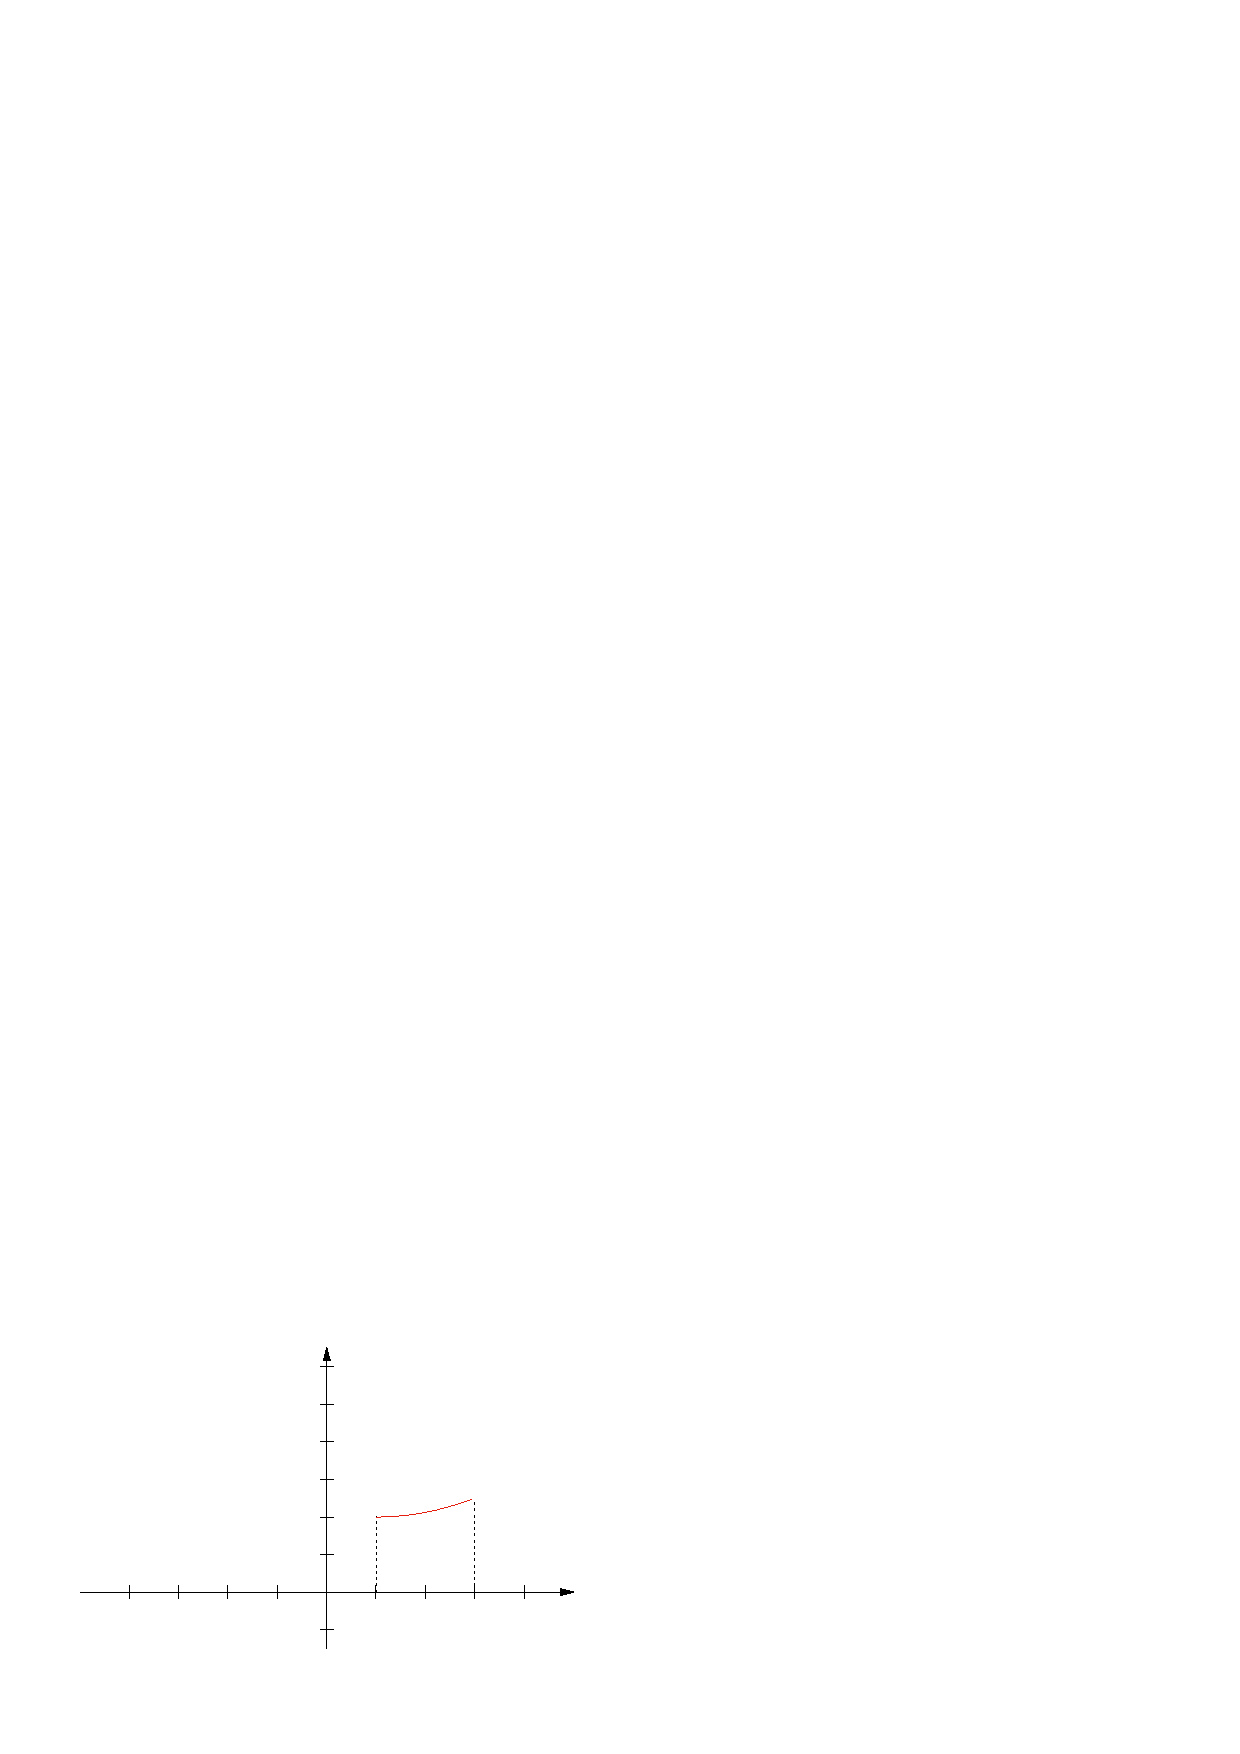
\includegraphics[width={216.00bp},height={144.00bp}]{figura_03_10}}%
    \gplfronttext
  \end{picture}%
\endgroup

\end{figure}

\section{La función impulso}
Pulso rectangular de área igual a 1.

\begin{figure}[H]
    \centering
    % GNUPLOT: LaTeX picture with Postscript
\begingroup
  \makeatletter
  \providecommand\color[2][]{%
    \GenericError{(gnuplot) \space\space\space\@spaces}{%
      Package color not loaded in conjunction with
      terminal option `colourtext'%
    }{See the gnuplot documentation for explanation.%
    }{Either use 'blacktext' in gnuplot or load the package
      color.sty in LaTeX.}%
    \renewcommand\color[2][]{}%
  }%
  \providecommand\includegraphics[2][]{%
    \GenericError{(gnuplot) \space\space\space\@spaces}{%
      Package graphicx or graphics not loaded%
    }{See the gnuplot documentation for explanation.%
    }{The gnuplot epslatex terminal needs graphicx.sty or graphics.sty.}%
    \renewcommand\includegraphics[2][]{}%
  }%
  \providecommand\rotatebox[2]{#2}%
  \@ifundefined{ifGPcolor}{%
    \newif\ifGPcolor
    \GPcolorfalse
  }{}%
  \@ifundefined{ifGPblacktext}{%
    \newif\ifGPblacktext
    \GPblacktexttrue
  }{}%
  % define a \g@addto@macro without @ in the name:
  \let\gplgaddtomacro\g@addto@macro
  % define empty templates for all commands taking text:
  \gdef\gplbacktext{}%
  \gdef\gplfronttext{}%
  \makeatother
  \ifGPblacktext
    % no textcolor at all
    \def\colorrgb#1{}%
    \def\colorgray#1{}%
  \else
    % gray or color?
    \ifGPcolor
      \def\colorrgb#1{\color[rgb]{#1}}%
      \def\colorgray#1{\color[gray]{#1}}%
      \expandafter\def\csname LTw\endcsname{\color{white}}%
      \expandafter\def\csname LTb\endcsname{\color{black}}%
      \expandafter\def\csname LTa\endcsname{\color{black}}%
      \expandafter\def\csname LT0\endcsname{\color[rgb]{1,0,0}}%
      \expandafter\def\csname LT1\endcsname{\color[rgb]{0,1,0}}%
      \expandafter\def\csname LT2\endcsname{\color[rgb]{0,0,1}}%
      \expandafter\def\csname LT3\endcsname{\color[rgb]{1,0,1}}%
      \expandafter\def\csname LT4\endcsname{\color[rgb]{0,1,1}}%
      \expandafter\def\csname LT5\endcsname{\color[rgb]{1,1,0}}%
      \expandafter\def\csname LT6\endcsname{\color[rgb]{0,0,0}}%
      \expandafter\def\csname LT7\endcsname{\color[rgb]{1,0.3,0}}%
      \expandafter\def\csname LT8\endcsname{\color[rgb]{0.5,0.5,0.5}}%
    \else
      % gray
      \def\colorrgb#1{\color{black}}%
      \def\colorgray#1{\color[gray]{#1}}%
      \expandafter\def\csname LTw\endcsname{\color{white}}%
      \expandafter\def\csname LTb\endcsname{\color{black}}%
      \expandafter\def\csname LTa\endcsname{\color{black}}%
      \expandafter\def\csname LT0\endcsname{\color{black}}%
      \expandafter\def\csname LT1\endcsname{\color{black}}%
      \expandafter\def\csname LT2\endcsname{\color{black}}%
      \expandafter\def\csname LT3\endcsname{\color{black}}%
      \expandafter\def\csname LT4\endcsname{\color{black}}%
      \expandafter\def\csname LT5\endcsname{\color{black}}%
      \expandafter\def\csname LT6\endcsname{\color{black}}%
      \expandafter\def\csname LT7\endcsname{\color{black}}%
      \expandafter\def\csname LT8\endcsname{\color{black}}%
    \fi
  \fi
    \setlength{\unitlength}{0.0500bp}%
    \ifx\gptboxheight\undefined%
      \newlength{\gptboxheight}%
      \newlength{\gptboxwidth}%
      \newsavebox{\gptboxtext}%
    \fi%
    \setlength{\fboxrule}{0.5pt}%
    \setlength{\fboxsep}{1pt}%
    \definecolor{tbcol}{rgb}{1,1,1}%
\begin{picture}(2160.00,2160.00)%
    \gplgaddtomacro\gplbacktext{%
      \csname LTb\endcsname%%
      \put(960,192){\makebox(0,0)[r]{\strut{}}}%
      \put(960,644){\makebox(0,0)[r]{\strut{}}}%
      \put(960,1096){\makebox(0,0)[r]{\strut{}}}%
      \put(960,1547){\makebox(0,0)[r]{\strut{}}}%
      \put(960,1999){\makebox(0,0)[r]{\strut{}}}%
      \put(240,421){\makebox(0,0){\strut{}}}%
      \put(648,421){\makebox(0,0){\strut{}}}%
      \put(1056,421){\makebox(0,0){\strut{}}}%
      \put(1463,421){\makebox(0,0){\strut{}}}%
      \put(1871,421){\makebox(0,0){\strut{}}}%
      \csname LTb\endcsname%%
      \put(2279,644){\makebox(0,0)[l]{\strut{}$t$}}%
      \put(1239,2180){\makebox(0,0)[l]{\strut{}$f(t)$}}%
      \put(1422,373){\makebox(0,0)[l]{\strut{}$\xi$}}%
      \put(444,373){\makebox(0,0)[l]{\strut{}$-\xi$}}%
      \put(1626,1547){\makebox(0,0)[l]{\strut{}$\dfrac{1}{2\xi}$}}%
    }%
    \gplgaddtomacro\gplfronttext{%
    }%
    \gplbacktext
    \put(0,0){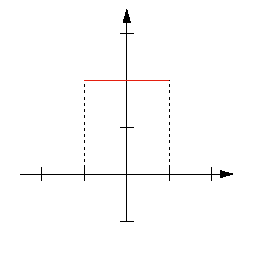
\includegraphics[width={108.00bp},height={108.00bp}]{figura_03_11}}%
    \gplfronttext
  \end{picture}%
\endgroup

\end{figure}

Si $\xi\to0$, entonces $\frac{1}{2\xi}\to\infty$.

\begin{figure}[H]
    \centering
    % GNUPLOT: LaTeX picture with Postscript
\begingroup
  \makeatletter
  \providecommand\color[2][]{%
    \GenericError{(gnuplot) \space\space\space\@spaces}{%
      Package color not loaded in conjunction with
      terminal option `colourtext'%
    }{See the gnuplot documentation for explanation.%
    }{Either use 'blacktext' in gnuplot or load the package
      color.sty in LaTeX.}%
    \renewcommand\color[2][]{}%
  }%
  \providecommand\includegraphics[2][]{%
    \GenericError{(gnuplot) \space\space\space\@spaces}{%
      Package graphicx or graphics not loaded%
    }{See the gnuplot documentation for explanation.%
    }{The gnuplot epslatex terminal needs graphicx.sty or graphics.sty.}%
    \renewcommand\includegraphics[2][]{}%
  }%
  \providecommand\rotatebox[2]{#2}%
  \@ifundefined{ifGPcolor}{%
    \newif\ifGPcolor
    \GPcolorfalse
  }{}%
  \@ifundefined{ifGPblacktext}{%
    \newif\ifGPblacktext
    \GPblacktexttrue
  }{}%
  % define a \g@addto@macro without @ in the name:
  \let\gplgaddtomacro\g@addto@macro
  % define empty templates for all commands taking text:
  \gdef\gplbacktext{}%
  \gdef\gplfronttext{}%
  \makeatother
  \ifGPblacktext
    % no textcolor at all
    \def\colorrgb#1{}%
    \def\colorgray#1{}%
  \else
    % gray or color?
    \ifGPcolor
      \def\colorrgb#1{\color[rgb]{#1}}%
      \def\colorgray#1{\color[gray]{#1}}%
      \expandafter\def\csname LTw\endcsname{\color{white}}%
      \expandafter\def\csname LTb\endcsname{\color{black}}%
      \expandafter\def\csname LTa\endcsname{\color{black}}%
      \expandafter\def\csname LT0\endcsname{\color[rgb]{1,0,0}}%
      \expandafter\def\csname LT1\endcsname{\color[rgb]{0,1,0}}%
      \expandafter\def\csname LT2\endcsname{\color[rgb]{0,0,1}}%
      \expandafter\def\csname LT3\endcsname{\color[rgb]{1,0,1}}%
      \expandafter\def\csname LT4\endcsname{\color[rgb]{0,1,1}}%
      \expandafter\def\csname LT5\endcsname{\color[rgb]{1,1,0}}%
      \expandafter\def\csname LT6\endcsname{\color[rgb]{0,0,0}}%
      \expandafter\def\csname LT7\endcsname{\color[rgb]{1,0.3,0}}%
      \expandafter\def\csname LT8\endcsname{\color[rgb]{0.5,0.5,0.5}}%
    \else
      % gray
      \def\colorrgb#1{\color{black}}%
      \def\colorgray#1{\color[gray]{#1}}%
      \expandafter\def\csname LTw\endcsname{\color{white}}%
      \expandafter\def\csname LTb\endcsname{\color{black}}%
      \expandafter\def\csname LTa\endcsname{\color{black}}%
      \expandafter\def\csname LT0\endcsname{\color{black}}%
      \expandafter\def\csname LT1\endcsname{\color{black}}%
      \expandafter\def\csname LT2\endcsname{\color{black}}%
      \expandafter\def\csname LT3\endcsname{\color{black}}%
      \expandafter\def\csname LT4\endcsname{\color{black}}%
      \expandafter\def\csname LT5\endcsname{\color{black}}%
      \expandafter\def\csname LT6\endcsname{\color{black}}%
      \expandafter\def\csname LT7\endcsname{\color{black}}%
      \expandafter\def\csname LT8\endcsname{\color{black}}%
    \fi
  \fi
    \setlength{\unitlength}{0.0500bp}%
    \ifx\gptboxheight\undefined%
      \newlength{\gptboxheight}%
      \newlength{\gptboxwidth}%
      \newsavebox{\gptboxtext}%
    \fi%
    \setlength{\fboxrule}{0.5pt}%
    \setlength{\fboxsep}{1pt}%
    \definecolor{tbcol}{rgb}{1,1,1}%
\begin{picture}(2160.00,2160.00)%
    \gplgaddtomacro\gplbacktext{%
      \csname LTb\endcsname%%
      \put(960,192){\makebox(0,0)[r]{\strut{}}}%
      \put(960,644){\makebox(0,0)[r]{\strut{}}}%
      \put(960,1096){\makebox(0,0)[r]{\strut{}}}%
      \put(960,1547){\makebox(0,0)[r]{\strut{}}}%
      \put(960,1999){\makebox(0,0)[r]{\strut{}}}%
      \put(240,421){\makebox(0,0){\strut{}}}%
      \put(648,421){\makebox(0,0){\strut{}}}%
      \put(1056,421){\makebox(0,0){\strut{}}}%
      \put(1463,421){\makebox(0,0){\strut{}}}%
      \put(1871,421){\makebox(0,0){\strut{}}}%
      \csname LTb\endcsname%%
      \put(2279,644){\makebox(0,0)[l]{\strut{}$t$}}%
      \put(1239,2180){\makebox(0,0)[l]{\strut{}$f(t)$}}%
      \put(1219,1547){\makebox(0,0)[l]{\strut{}$\delta(t)$}}%
    }%
    \gplgaddtomacro\gplfronttext{%
    }%
    \gplbacktext
    \put(0,0){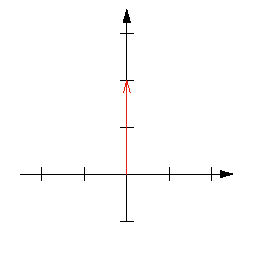
\includegraphics[width={108.00bp},height={108.00bp}]{figura_03_12}}%
    \gplfronttext
  \end{picture}%
\endgroup

\end{figure}

\begin{equation*}
    \delta(t)=\begin{cases}
        0      & t\neq0\\
        \infty & t=0\\
    \end{cases}
\end{equation*}

Tal que:

\begin{equation*}
    \int_{-\xi}^{\xi} \delta(t)\,dt=1
\end{equation*}

Por tanto:

\begin{equation*}
    k\delta(t)=\begin{cases}
        0         & t\neq0\\
        \pm\infty & t=0\\
    \end{cases}
\end{equation*}

\begin{figure}[H]
    \centering
    % GNUPLOT: LaTeX picture with Postscript
\begingroup
  \makeatletter
  \providecommand\color[2][]{%
    \GenericError{(gnuplot) \space\space\space\@spaces}{%
      Package color not loaded in conjunction with
      terminal option `colourtext'%
    }{See the gnuplot documentation for explanation.%
    }{Either use 'blacktext' in gnuplot or load the package
      color.sty in LaTeX.}%
    \renewcommand\color[2][]{}%
  }%
  \providecommand\includegraphics[2][]{%
    \GenericError{(gnuplot) \space\space\space\@spaces}{%
      Package graphicx or graphics not loaded%
    }{See the gnuplot documentation for explanation.%
    }{The gnuplot epslatex terminal needs graphicx.sty or graphics.sty.}%
    \renewcommand\includegraphics[2][]{}%
  }%
  \providecommand\rotatebox[2]{#2}%
  \@ifundefined{ifGPcolor}{%
    \newif\ifGPcolor
    \GPcolorfalse
  }{}%
  \@ifundefined{ifGPblacktext}{%
    \newif\ifGPblacktext
    \GPblacktexttrue
  }{}%
  % define a \g@addto@macro without @ in the name:
  \let\gplgaddtomacro\g@addto@macro
  % define empty templates for all commands taking text:
  \gdef\gplbacktext{}%
  \gdef\gplfronttext{}%
  \makeatother
  \ifGPblacktext
    % no textcolor at all
    \def\colorrgb#1{}%
    \def\colorgray#1{}%
  \else
    % gray or color?
    \ifGPcolor
      \def\colorrgb#1{\color[rgb]{#1}}%
      \def\colorgray#1{\color[gray]{#1}}%
      \expandafter\def\csname LTw\endcsname{\color{white}}%
      \expandafter\def\csname LTb\endcsname{\color{black}}%
      \expandafter\def\csname LTa\endcsname{\color{black}}%
      \expandafter\def\csname LT0\endcsname{\color[rgb]{1,0,0}}%
      \expandafter\def\csname LT1\endcsname{\color[rgb]{0,1,0}}%
      \expandafter\def\csname LT2\endcsname{\color[rgb]{0,0,1}}%
      \expandafter\def\csname LT3\endcsname{\color[rgb]{1,0,1}}%
      \expandafter\def\csname LT4\endcsname{\color[rgb]{0,1,1}}%
      \expandafter\def\csname LT5\endcsname{\color[rgb]{1,1,0}}%
      \expandafter\def\csname LT6\endcsname{\color[rgb]{0,0,0}}%
      \expandafter\def\csname LT7\endcsname{\color[rgb]{1,0.3,0}}%
      \expandafter\def\csname LT8\endcsname{\color[rgb]{0.5,0.5,0.5}}%
    \else
      % gray
      \def\colorrgb#1{\color{black}}%
      \def\colorgray#1{\color[gray]{#1}}%
      \expandafter\def\csname LTw\endcsname{\color{white}}%
      \expandafter\def\csname LTb\endcsname{\color{black}}%
      \expandafter\def\csname LTa\endcsname{\color{black}}%
      \expandafter\def\csname LT0\endcsname{\color{black}}%
      \expandafter\def\csname LT1\endcsname{\color{black}}%
      \expandafter\def\csname LT2\endcsname{\color{black}}%
      \expandafter\def\csname LT3\endcsname{\color{black}}%
      \expandafter\def\csname LT4\endcsname{\color{black}}%
      \expandafter\def\csname LT5\endcsname{\color{black}}%
      \expandafter\def\csname LT6\endcsname{\color{black}}%
      \expandafter\def\csname LT7\endcsname{\color{black}}%
      \expandafter\def\csname LT8\endcsname{\color{black}}%
    \fi
  \fi
    \setlength{\unitlength}{0.0500bp}%
    \ifx\gptboxheight\undefined%
      \newlength{\gptboxheight}%
      \newlength{\gptboxwidth}%
      \newsavebox{\gptboxtext}%
    \fi%
    \setlength{\fboxrule}{0.5pt}%
    \setlength{\fboxsep}{1pt}%
    \definecolor{tbcol}{rgb}{1,1,1}%
\begin{picture}(2160.00,2160.00)%
    \gplgaddtomacro\gplbacktext{%
      \csname LTb\endcsname%%
      \put(960,192){\makebox(0,0)[r]{\strut{}}}%
      \put(960,644){\makebox(0,0)[r]{\strut{}}}%
      \put(960,1096){\makebox(0,0)[r]{\strut{}}}%
      \put(960,1547){\makebox(0,0)[r]{\strut{}}}%
      \put(960,1999){\makebox(0,0)[r]{\strut{}}}%
      \put(240,421){\makebox(0,0){\strut{}}}%
      \put(648,421){\makebox(0,0){\strut{}}}%
      \put(1056,421){\makebox(0,0){\strut{}}}%
      \put(1463,421){\makebox(0,0){\strut{}}}%
      \put(1871,421){\makebox(0,0){\strut{}}}%
      \csname LTb\endcsname%%
      \put(2279,644){\makebox(0,0)[l]{\strut{}$t$}}%
      \put(1239,2180){\makebox(0,0)[l]{\strut{}$f(t)$}}%
      \put(1626,1547){\makebox(0,0)[l]{\strut{}$k\delta(t-t_0)$}}%
      \put(1626,1276){\makebox(0,0)[l]{\strut{}$k>0$}}%
      \put(1422,463){\makebox(0,0)[l]{\strut{}$t_0$}}%
    }%
    \gplgaddtomacro\gplfronttext{%
    }%
    \gplbacktext
    \put(0,0){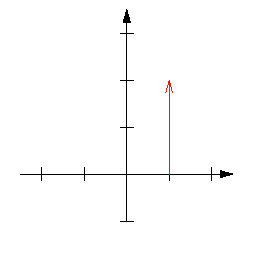
\includegraphics[width={108.00bp},height={108.00bp}]{figura_03_13}}%
    \gplfronttext
  \end{picture}%
\endgroup

\end{figure}

\begin{figure}[H]
    \centering
    % GNUPLOT: LaTeX picture with Postscript
\begingroup
  \makeatletter
  \providecommand\color[2][]{%
    \GenericError{(gnuplot) \space\space\space\@spaces}{%
      Package color not loaded in conjunction with
      terminal option `colourtext'%
    }{See the gnuplot documentation for explanation.%
    }{Either use 'blacktext' in gnuplot or load the package
      color.sty in LaTeX.}%
    \renewcommand\color[2][]{}%
  }%
  \providecommand\includegraphics[2][]{%
    \GenericError{(gnuplot) \space\space\space\@spaces}{%
      Package graphicx or graphics not loaded%
    }{See the gnuplot documentation for explanation.%
    }{The gnuplot epslatex terminal needs graphicx.sty or graphics.sty.}%
    \renewcommand\includegraphics[2][]{}%
  }%
  \providecommand\rotatebox[2]{#2}%
  \@ifundefined{ifGPcolor}{%
    \newif\ifGPcolor
    \GPcolorfalse
  }{}%
  \@ifundefined{ifGPblacktext}{%
    \newif\ifGPblacktext
    \GPblacktexttrue
  }{}%
  % define a \g@addto@macro without @ in the name:
  \let\gplgaddtomacro\g@addto@macro
  % define empty templates for all commands taking text:
  \gdef\gplbacktext{}%
  \gdef\gplfronttext{}%
  \makeatother
  \ifGPblacktext
    % no textcolor at all
    \def\colorrgb#1{}%
    \def\colorgray#1{}%
  \else
    % gray or color?
    \ifGPcolor
      \def\colorrgb#1{\color[rgb]{#1}}%
      \def\colorgray#1{\color[gray]{#1}}%
      \expandafter\def\csname LTw\endcsname{\color{white}}%
      \expandafter\def\csname LTb\endcsname{\color{black}}%
      \expandafter\def\csname LTa\endcsname{\color{black}}%
      \expandafter\def\csname LT0\endcsname{\color[rgb]{1,0,0}}%
      \expandafter\def\csname LT1\endcsname{\color[rgb]{0,1,0}}%
      \expandafter\def\csname LT2\endcsname{\color[rgb]{0,0,1}}%
      \expandafter\def\csname LT3\endcsname{\color[rgb]{1,0,1}}%
      \expandafter\def\csname LT4\endcsname{\color[rgb]{0,1,1}}%
      \expandafter\def\csname LT5\endcsname{\color[rgb]{1,1,0}}%
      \expandafter\def\csname LT6\endcsname{\color[rgb]{0,0,0}}%
      \expandafter\def\csname LT7\endcsname{\color[rgb]{1,0.3,0}}%
      \expandafter\def\csname LT8\endcsname{\color[rgb]{0.5,0.5,0.5}}%
    \else
      % gray
      \def\colorrgb#1{\color{black}}%
      \def\colorgray#1{\color[gray]{#1}}%
      \expandafter\def\csname LTw\endcsname{\color{white}}%
      \expandafter\def\csname LTb\endcsname{\color{black}}%
      \expandafter\def\csname LTa\endcsname{\color{black}}%
      \expandafter\def\csname LT0\endcsname{\color{black}}%
      \expandafter\def\csname LT1\endcsname{\color{black}}%
      \expandafter\def\csname LT2\endcsname{\color{black}}%
      \expandafter\def\csname LT3\endcsname{\color{black}}%
      \expandafter\def\csname LT4\endcsname{\color{black}}%
      \expandafter\def\csname LT5\endcsname{\color{black}}%
      \expandafter\def\csname LT6\endcsname{\color{black}}%
      \expandafter\def\csname LT7\endcsname{\color{black}}%
      \expandafter\def\csname LT8\endcsname{\color{black}}%
    \fi
  \fi
    \setlength{\unitlength}{0.0500bp}%
    \ifx\gptboxheight\undefined%
      \newlength{\gptboxheight}%
      \newlength{\gptboxwidth}%
      \newsavebox{\gptboxtext}%
    \fi%
    \setlength{\fboxrule}{0.5pt}%
    \setlength{\fboxsep}{1pt}%
    \definecolor{tbcol}{rgb}{1,1,1}%
\begin{picture}(2160.00,2160.00)%
    \gplgaddtomacro\gplbacktext{%
      \csname LTb\endcsname%%
      \put(960,192){\makebox(0,0)[r]{\strut{}}}%
      \put(960,644){\makebox(0,0)[r]{\strut{}}}%
      \put(960,1096){\makebox(0,0)[r]{\strut{}}}%
      \put(960,1547){\makebox(0,0)[r]{\strut{}}}%
      \put(960,1999){\makebox(0,0)[r]{\strut{}}}%
      \put(240,1324){\makebox(0,0){\strut{}}}%
      \put(648,1324){\makebox(0,0){\strut{}}}%
      \put(1056,1324){\makebox(0,0){\strut{}}}%
      \put(1463,1324){\makebox(0,0){\strut{}}}%
      \put(1871,1324){\makebox(0,0){\strut{}}}%
      \csname LTb\endcsname%%
      \put(2279,1547){\makebox(0,0)[l]{\strut{}$t$}}%
      \put(1239,2180){\makebox(0,0)[l]{\strut{}$f(t)$}}%
      \put(1626,644){\makebox(0,0)[l]{\strut{}$k\delta(t-t_0)$}}%
      \put(1626,915){\makebox(0,0)[l]{\strut{}$k<0$}}%
      \put(1422,1728){\makebox(0,0)[l]{\strut{}$t_0$}}%
    }%
    \gplgaddtomacro\gplfronttext{%
    }%
    \gplbacktext
    \put(0,0){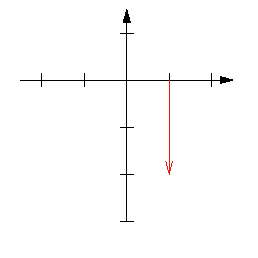
\includegraphics[width={108.00bp},height={108.00bp}]{figura_03_14}}%
    \gplfronttext
  \end{picture}%
\endgroup

\end{figure}

Si: $\phi(t)$ es una función de prueba:

\begin{equation*}
    \phi(t)\delta(t-t_0)=\phi(t_0)\delta(t-t_0)
\end{equation*}

\begin{figure}[H]
    \centering
    % GNUPLOT: LaTeX picture with Postscript
\begingroup
  \makeatletter
  \providecommand\color[2][]{%
    \GenericError{(gnuplot) \space\space\space\@spaces}{%
      Package color not loaded in conjunction with
      terminal option `colourtext'%
    }{See the gnuplot documentation for explanation.%
    }{Either use 'blacktext' in gnuplot or load the package
      color.sty in LaTeX.}%
    \renewcommand\color[2][]{}%
  }%
  \providecommand\includegraphics[2][]{%
    \GenericError{(gnuplot) \space\space\space\@spaces}{%
      Package graphicx or graphics not loaded%
    }{See the gnuplot documentation for explanation.%
    }{The gnuplot epslatex terminal needs graphicx.sty or graphics.sty.}%
    \renewcommand\includegraphics[2][]{}%
  }%
  \providecommand\rotatebox[2]{#2}%
  \@ifundefined{ifGPcolor}{%
    \newif\ifGPcolor
    \GPcolorfalse
  }{}%
  \@ifundefined{ifGPblacktext}{%
    \newif\ifGPblacktext
    \GPblacktexttrue
  }{}%
  % define a \g@addto@macro without @ in the name:
  \let\gplgaddtomacro\g@addto@macro
  % define empty templates for all commands taking text:
  \gdef\gplbacktext{}%
  \gdef\gplfronttext{}%
  \makeatother
  \ifGPblacktext
    % no textcolor at all
    \def\colorrgb#1{}%
    \def\colorgray#1{}%
  \else
    % gray or color?
    \ifGPcolor
      \def\colorrgb#1{\color[rgb]{#1}}%
      \def\colorgray#1{\color[gray]{#1}}%
      \expandafter\def\csname LTw\endcsname{\color{white}}%
      \expandafter\def\csname LTb\endcsname{\color{black}}%
      \expandafter\def\csname LTa\endcsname{\color{black}}%
      \expandafter\def\csname LT0\endcsname{\color[rgb]{1,0,0}}%
      \expandafter\def\csname LT1\endcsname{\color[rgb]{0,1,0}}%
      \expandafter\def\csname LT2\endcsname{\color[rgb]{0,0,1}}%
      \expandafter\def\csname LT3\endcsname{\color[rgb]{1,0,1}}%
      \expandafter\def\csname LT4\endcsname{\color[rgb]{0,1,1}}%
      \expandafter\def\csname LT5\endcsname{\color[rgb]{1,1,0}}%
      \expandafter\def\csname LT6\endcsname{\color[rgb]{0,0,0}}%
      \expandafter\def\csname LT7\endcsname{\color[rgb]{1,0.3,0}}%
      \expandafter\def\csname LT8\endcsname{\color[rgb]{0.5,0.5,0.5}}%
    \else
      % gray
      \def\colorrgb#1{\color{black}}%
      \def\colorgray#1{\color[gray]{#1}}%
      \expandafter\def\csname LTw\endcsname{\color{white}}%
      \expandafter\def\csname LTb\endcsname{\color{black}}%
      \expandafter\def\csname LTa\endcsname{\color{black}}%
      \expandafter\def\csname LT0\endcsname{\color{black}}%
      \expandafter\def\csname LT1\endcsname{\color{black}}%
      \expandafter\def\csname LT2\endcsname{\color{black}}%
      \expandafter\def\csname LT3\endcsname{\color{black}}%
      \expandafter\def\csname LT4\endcsname{\color{black}}%
      \expandafter\def\csname LT5\endcsname{\color{black}}%
      \expandafter\def\csname LT6\endcsname{\color{black}}%
      \expandafter\def\csname LT7\endcsname{\color{black}}%
      \expandafter\def\csname LT8\endcsname{\color{black}}%
    \fi
  \fi
    \setlength{\unitlength}{0.0500bp}%
    \ifx\gptboxheight\undefined%
      \newlength{\gptboxheight}%
      \newlength{\gptboxwidth}%
      \newsavebox{\gptboxtext}%
    \fi%
    \setlength{\fboxrule}{0.5pt}%
    \setlength{\fboxsep}{1pt}%
    \definecolor{tbcol}{rgb}{1,1,1}%
\begin{picture}(4320.00,2880.00)%
    \gplgaddtomacro\gplbacktext{%
      \csname LTb\endcsname%%
      \put(2040,192){\makebox(0,0)[r]{\strut{}}}%
      \put(2040,553){\makebox(0,0)[r]{\strut{}}}%
      \put(2040,914){\makebox(0,0)[r]{\strut{}}}%
      \put(2040,1275){\makebox(0,0)[r]{\strut{}}}%
      \put(2040,1636){\makebox(0,0)[r]{\strut{}}}%
      \put(2040,1997){\makebox(0,0)[r]{\strut{}}}%
      \put(2040,2358){\makebox(0,0)[r]{\strut{}}}%
      \put(2040,2719){\makebox(0,0)[r]{\strut{}}}%
      \put(240,330){\makebox(0,0){\strut{}}}%
      \put(714,330){\makebox(0,0){\strut{}}}%
      \put(1188,330){\makebox(0,0){\strut{}}}%
      \put(1662,330){\makebox(0,0){\strut{}}}%
      \put(2136,330){\makebox(0,0){\strut{}}}%
      \put(2609,330){\makebox(0,0){\strut{}}}%
      \put(3083,330){\makebox(0,0){\strut{}}}%
      \put(3557,330){\makebox(0,0){\strut{}}}%
      \put(4031,330){\makebox(0,0){\strut{}}}%
      \csname LTb\endcsname%%
      \put(4647,553){\makebox(0,0)[l]{\strut{}$t$}}%
      \put(2349,2863){\makebox(0,0)[l]{\strut{}$f(t)$}}%
      \put(2562,336){\makebox(0,0)[l]{\strut{}$t_0$}}%
      \put(1235,1275){\makebox(0,0)[l]{\strut{}$\phi(t_0)$}}%
      \put(714,2178){\makebox(0,0)[l]{\strut{}$\phi(t)$}}%
      \put(2799,2178){\makebox(0,0)[l]{\strut{}$\delta(t-t_0)$}}%
    }%
    \gplgaddtomacro\gplfronttext{%
    }%
    \gplbacktext
    \put(0,0){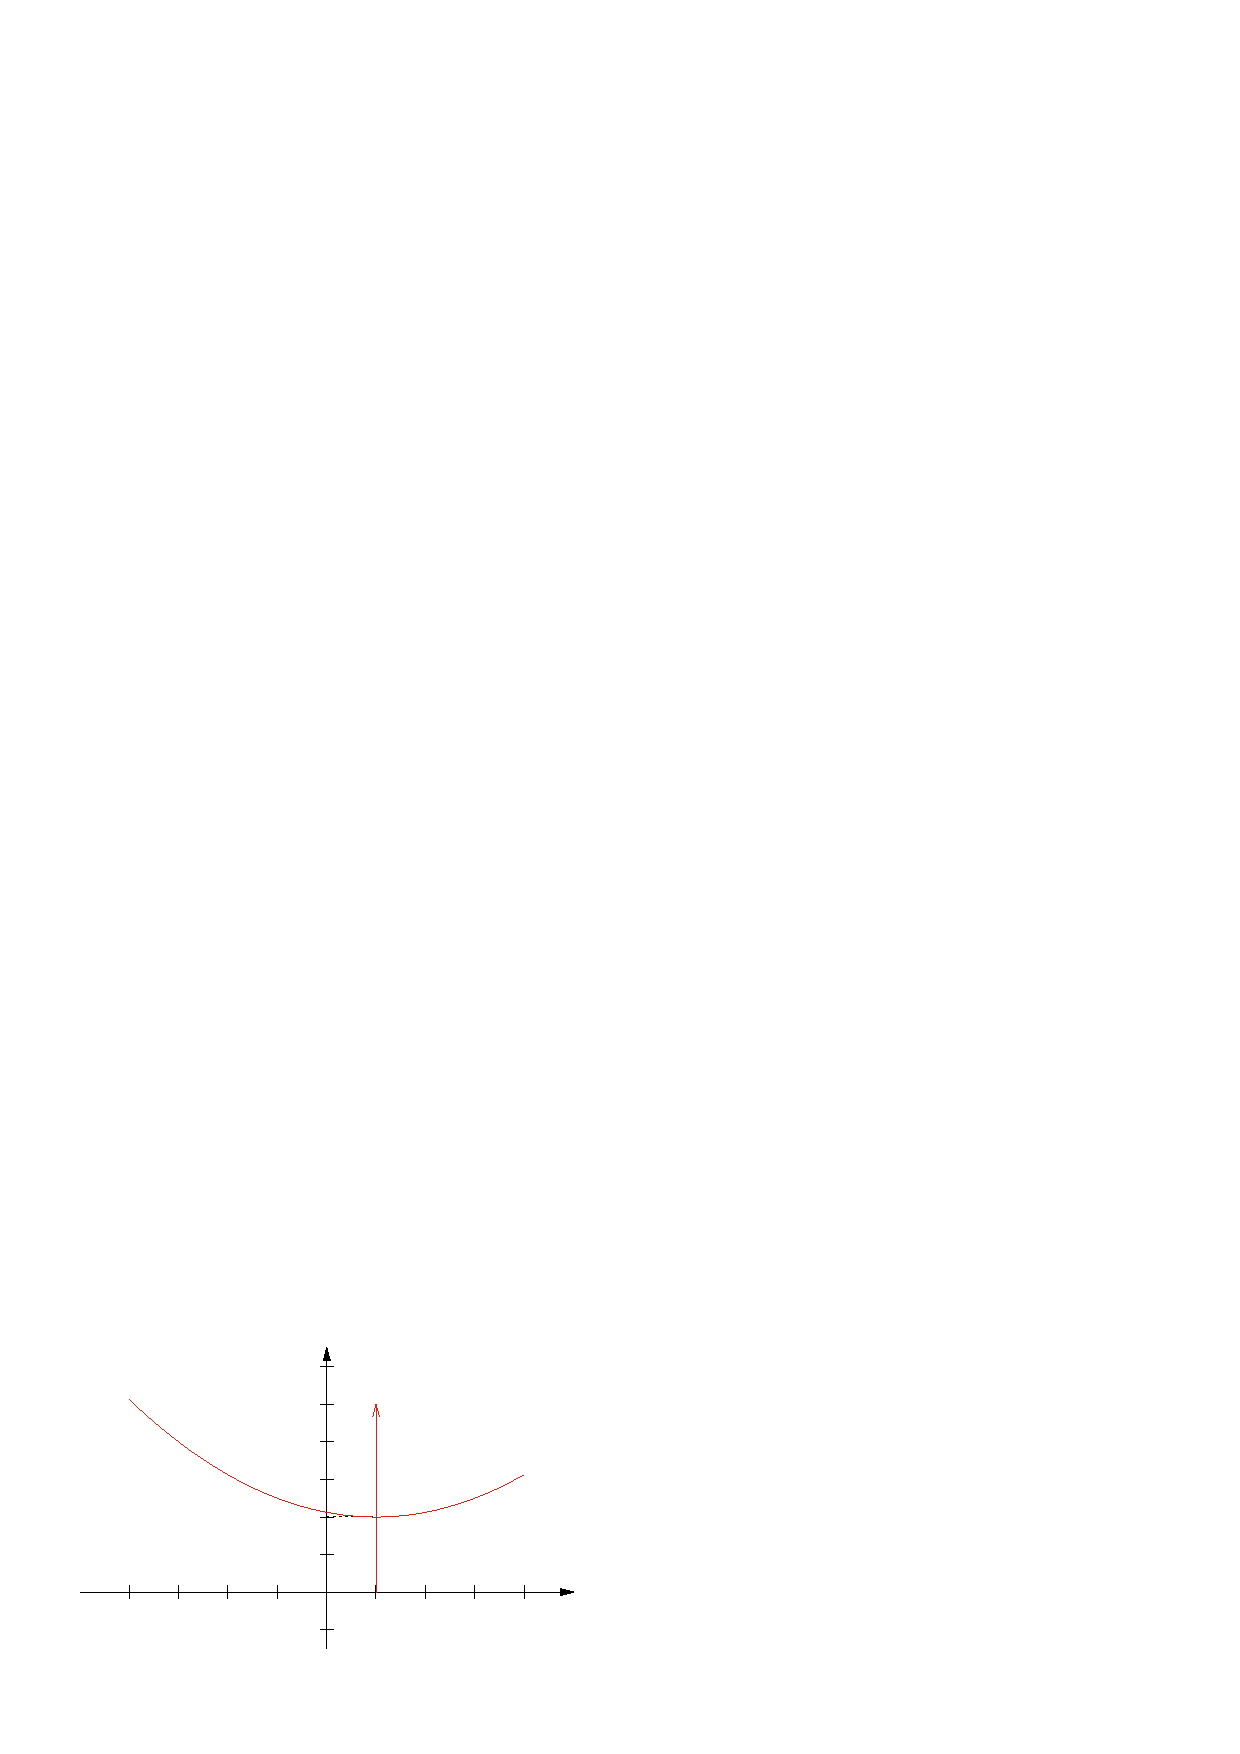
\includegraphics[width={216.00bp},height={144.00bp}]{figura_03_15}}%
    \gplfronttext
  \end{picture}%
\endgroup

\end{figure}

Para $t\neq0$

\begin{equation*}
    \phi(t)\delta(t-t_0)=0
\end{equation*}

Para $t=0$

\begin{equation*}
    \phi(t)\delta(t-t_0)=\phi(t_0)\delta(t-t_0)
\end{equation*}

\subsection{Propiedades de la función impulso}

\subsubsection*{Propiedad 1}

\begin{equation*}
    \int_a^b \delta(t-t_0)\,dt=\begin{cases}
        1 & t_0\in[a,b] \\
        0 & t_0\notin[a,b] \\
    \end{cases}
\end{equation*}

En general:

\begin{equation*}
    \int_{-\infty}^{\infty}\delta(t-t_0)\,dt=1
\end{equation*}

\subsubsection*{Propiedad 2}

\begin{equation*}
    \int_a^b \phi(t)\,\delta(t-t_0)\,dt=\begin{cases}
        \phi(t_0) & t_0\in[a,b] \\
        0 & t_0\notin[a,b] \\
    \end{cases}
\end{equation*}

En general:

\begin{equation*}
    \int_{-\infty}^{\infty}\phi(t_0)\,\delta(t-t_0)\,dt=\phi(t_0)
\end{equation*}

\underline{Prueba}:
\begin{equation*}
\begin{split}
    \int_{-\infty}^{\infty}\phi(t)\delta(t-t_0)\,dt
        &=\int_{-\infty}^{\infty}\phi(t_0)\delta(t-t_0)\,dt\\
        &=\phi(t_0)\int_{-\infty}^{\infty}\delta(t-t_0)\,dt\\
        &=\phi(t_0)\\
\end{split}
\end{equation*}

\subsubsection*{Propiedad 3}

\begin{equation*}
    \int_{-\infty}^{\infty}\phi(t)\,\delta(at)\,dt
        =\frac{1}{|a|}\int_{-\infty}^{\infty}
            \phi\left(\frac{t}{a}\right)\delta(t)\,dt
        =\frac{\phi(0)}{|a|}; a\neq0
\end{equation*}

\underline{Prueba}:

Realizando un cambio de variable:

\begin{equation*}
    \tau=at
\end{equation*}
\begin{equation*}
    d\tau=a\,dt
\end{equation*}

Para $a>0$:

\begin{equation*}
    \int_{-\infty}^{\infty}
        \phi\left(\frac{\tau}{a}\right)\delta(\tau)\,\frac{d\tau}{a}
        =\frac{1}{a}\int_{-\infty}^{\infty}
            \phi\left(\frac{\tau}{a}\right)\delta(\tau)d\tau
\end{equation*}

Para $a<0$:

\begin{equation*}
    \int_{-\infty}^{\infty}
        \phi\left(\frac{\tau}{a}\right)\delta(\tau)\,\frac{d\tau}{a}
        =-\frac{1}{a}\int_{-\infty}^{\infty}
            \phi\left(\frac{\tau}{a}\right)\delta(\tau)d\tau
\end{equation*}

Como:

\begin{equation*}
    |a|=\begin{cases}
        -a & a<0 \\
         a & a>0 \\
    \end{cases}
\end{equation*}

\begin{equation*}
\begin{split}
    \int_{-\infty}^{\infty}\phi(t)\,\delta(at)\,dt
        &=\frac{1}{|a|}\int_{-\infty}^{\infty}
            \phi\left(\frac{\tau}{a}\right)\delta(\tau)\,d\tau\\
        &=\frac{1}{|a|}\phi\left(\frac{0}{a}\right)\\
        &=\frac{\phi(0)}{|a|}\\
\end{split}
\end{equation*}

\subsubsection*{Propiedad 4}

\begin{equation*}
    \delta(at)=\frac{1}{|a|}\delta(t)
\end{equation*}

En particular:

\begin{equation*}
    \delta(-t)=\delta(t)
\end{equation*}

Por tanto $\delta(t)$ es una función \textbf{par}.

\underline{Prueba}:

\begin{equation*}
\begin{split}
    \int_{-\infty}^{\infty}\phi(t)\,\delta(at)\,dt
        &=\frac{1}{|a|}\phi(0)\\
        &=\frac{1}{|a|}\int_{-\infty}^{\infty}\phi(t)\,\delta(t)\,dt\\
\end{split}
\end{equation*}

\begin{equation*}
    \phi(t)\,\delta(at)=\frac{1}{|a|}\phi(t)\,\delta(t)
\end{equation*}

\begin{equation*}
    \delta(at)=\frac{1}{|a|}\,\delta(t)
\end{equation*}

Para $a=-1$:

\begin{equation*}
    \delta(-t)=\frac{1}{|-1|}\,\delta(t)=\delta(t)
\end{equation*}

\subsubsection*{Propiedad 5}

\begin{equation*}
    t\,\delta(t)=0
\end{equation*}
\begin{equation*}
    t^n\,\delta(t)=0; n\in\mathbb{N}
\end{equation*}

\underline{Prueba}:

\begin{equation*}
    \int_{-\infty}^{\infty}t^n\,\delta(t)\,dt=0^n=0
\end{equation*}

Derivando ambos miembros:

\begin{equation*}
    t^n\,\delta(t)\,dt=0
\end{equation*}

\section{Derivada de la función impulso}

\begin{equation*}
    \delta'(t)=\frac{d}{dt}(\delta(t))
\end{equation*}

\begin{equation*}
    \int_{-\infty}^{\infty}\phi(t)\delta'(t)\,dt
        =-\int_{-\infty}^{\infty}\phi'(t)\delta(t)\,dt
        =-\phi'(0)
\end{equation*}

\underline{Prueba}:

Realizando la integración por partes:

\begin{equation*}
    u=\phi(t)
\end{equation*}
\begin{equation*}
    du=\phi'(t)\,dt
\end{equation*}
\begin{equation*}
    dv=\delta'(t-t_0)\,dt
\end{equation*}
\begin{equation*}
    v=\delta(t-t_0)
\end{equation*}

\begin{equation*}
\begin{split}
    \int_{-\infty}^{\infty}\phi(t)\delta'(t-t_0)\,dt
        &=(\phi(t)\delta(t-t_0)\Big|_{-\infty}^{\infty})
        -\int_{-\infty}^{\infty}\delta(t-t_0)\phi'(t)\,dt\\
        &=0-\int_{-\infty}^{\infty}\delta(t-t_0)\phi'(t)\,dt\\
        &=-\phi'(t_0)
\end{split}
\end{equation*}

\subsubsection{Derivadas de orden superior}

\begin{equation*}
\begin{split}
    \int_{-\infty}^{\infty}\phi(t)\delta''(t)\,dt
        &=\int_{-\infty}^{\infty}\phi(t)(\delta'(t))'\,dt\\
        &=-\int_{-\infty}^{\infty}\phi'(t)\delta'(t)\,dt\\
        &=\int_{-\infty}^{\infty}\phi''(t)\delta(t)\,dt\\
        &=\phi''(0)\\
\end{split}
\end{equation*}

De igual manera:

\begin{equation*}
    \int_{-\infty}^{\infty}\phi(t)\delta'''(t-t_0)\,dt=-\phi'''(t_0)
\end{equation*}

En general:

\begin{equation*}
    \int_{-\infty}^{\infty}\phi(t)\delta^{(n)}(t-t_0)\,dt=(-1)^n\phi^{(n)}(t_0)
\end{equation*}

\section{Derivada de la función escalón unitario}

\begin{figure}[H]
    \centering
    % GNUPLOT: LaTeX picture with Postscript
\begingroup
  \makeatletter
  \providecommand\color[2][]{%
    \GenericError{(gnuplot) \space\space\space\@spaces}{%
      Package color not loaded in conjunction with
      terminal option `colourtext'%
    }{See the gnuplot documentation for explanation.%
    }{Either use 'blacktext' in gnuplot or load the package
      color.sty in LaTeX.}%
    \renewcommand\color[2][]{}%
  }%
  \providecommand\includegraphics[2][]{%
    \GenericError{(gnuplot) \space\space\space\@spaces}{%
      Package graphicx or graphics not loaded%
    }{See the gnuplot documentation for explanation.%
    }{The gnuplot epslatex terminal needs graphicx.sty or graphics.sty.}%
    \renewcommand\includegraphics[2][]{}%
  }%
  \providecommand\rotatebox[2]{#2}%
  \@ifundefined{ifGPcolor}{%
    \newif\ifGPcolor
    \GPcolorfalse
  }{}%
  \@ifundefined{ifGPblacktext}{%
    \newif\ifGPblacktext
    \GPblacktexttrue
  }{}%
  % define a \g@addto@macro without @ in the name:
  \let\gplgaddtomacro\g@addto@macro
  % define empty templates for all commands taking text:
  \gdef\gplbacktext{}%
  \gdef\gplfronttext{}%
  \makeatother
  \ifGPblacktext
    % no textcolor at all
    \def\colorrgb#1{}%
    \def\colorgray#1{}%
  \else
    % gray or color?
    \ifGPcolor
      \def\colorrgb#1{\color[rgb]{#1}}%
      \def\colorgray#1{\color[gray]{#1}}%
      \expandafter\def\csname LTw\endcsname{\color{white}}%
      \expandafter\def\csname LTb\endcsname{\color{black}}%
      \expandafter\def\csname LTa\endcsname{\color{black}}%
      \expandafter\def\csname LT0\endcsname{\color[rgb]{1,0,0}}%
      \expandafter\def\csname LT1\endcsname{\color[rgb]{0,1,0}}%
      \expandafter\def\csname LT2\endcsname{\color[rgb]{0,0,1}}%
      \expandafter\def\csname LT3\endcsname{\color[rgb]{1,0,1}}%
      \expandafter\def\csname LT4\endcsname{\color[rgb]{0,1,1}}%
      \expandafter\def\csname LT5\endcsname{\color[rgb]{1,1,0}}%
      \expandafter\def\csname LT6\endcsname{\color[rgb]{0,0,0}}%
      \expandafter\def\csname LT7\endcsname{\color[rgb]{1,0.3,0}}%
      \expandafter\def\csname LT8\endcsname{\color[rgb]{0.5,0.5,0.5}}%
    \else
      % gray
      \def\colorrgb#1{\color{black}}%
      \def\colorgray#1{\color[gray]{#1}}%
      \expandafter\def\csname LTw\endcsname{\color{white}}%
      \expandafter\def\csname LTb\endcsname{\color{black}}%
      \expandafter\def\csname LTa\endcsname{\color{black}}%
      \expandafter\def\csname LT0\endcsname{\color{black}}%
      \expandafter\def\csname LT1\endcsname{\color{black}}%
      \expandafter\def\csname LT2\endcsname{\color{black}}%
      \expandafter\def\csname LT3\endcsname{\color{black}}%
      \expandafter\def\csname LT4\endcsname{\color{black}}%
      \expandafter\def\csname LT5\endcsname{\color{black}}%
      \expandafter\def\csname LT6\endcsname{\color{black}}%
      \expandafter\def\csname LT7\endcsname{\color{black}}%
      \expandafter\def\csname LT8\endcsname{\color{black}}%
    \fi
  \fi
    \setlength{\unitlength}{0.0500bp}%
    \ifx\gptboxheight\undefined%
      \newlength{\gptboxheight}%
      \newlength{\gptboxwidth}%
      \newsavebox{\gptboxtext}%
    \fi%
    \setlength{\fboxrule}{0.5pt}%
    \setlength{\fboxsep}{1pt}%
    \definecolor{tbcol}{rgb}{1,1,1}%
\begin{picture}(2160.00,2160.00)%
    \gplgaddtomacro\gplbacktext{%
      \csname LTb\endcsname%%
      \put(960,192){\makebox(0,0)[r]{\strut{}}}%
      \put(960,644){\makebox(0,0)[r]{\strut{}}}%
      \put(960,1096){\makebox(0,0)[r]{\strut{}}}%
      \put(960,1547){\makebox(0,0)[r]{\strut{}}}%
      \put(960,1999){\makebox(0,0)[r]{\strut{}}}%
      \put(240,421){\makebox(0,0){\strut{}}}%
      \put(648,421){\makebox(0,0){\strut{}}}%
      \put(1056,421){\makebox(0,0){\strut{}}}%
      \put(1463,421){\makebox(0,0){\strut{}}}%
      \put(1871,421){\makebox(0,0){\strut{}}}%
      \csname LTb\endcsname%%
      \put(2279,644){\makebox(0,0)[l]{\strut{}$t$}}%
      \put(1239,2180){\makebox(0,0)[l]{\strut{}$f(t)$}}%
      \put(1219,1547){\makebox(0,0)[l]{\strut{}$\delta(t)$}}%
    }%
    \gplgaddtomacro\gplfronttext{%
    }%
    \gplbacktext
    \put(0,0){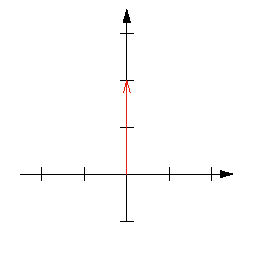
\includegraphics[width={108.00bp},height={108.00bp}]{figura_03_12}}%
    \gplfronttext
  \end{picture}%
\endgroup

\end{figure}


\chapter{Transformada de \emph{Fourier}}

\section{Integrales de \emph{Fourier}}
\begin{figure}[H]
    \centering
    % GNUPLOT: LaTeX picture with Postscript
\begingroup
  \makeatletter
  \providecommand\color[2][]{%
    \GenericError{(gnuplot) \space\space\space\@spaces}{%
      Package color not loaded in conjunction with
      terminal option `colourtext'%
    }{See the gnuplot documentation for explanation.%
    }{Either use 'blacktext' in gnuplot or load the package
      color.sty in LaTeX.}%
    \renewcommand\color[2][]{}%
  }%
  \providecommand\includegraphics[2][]{%
    \GenericError{(gnuplot) \space\space\space\@spaces}{%
      Package graphicx or graphics not loaded%
    }{See the gnuplot documentation for explanation.%
    }{The gnuplot epslatex terminal needs graphicx.sty or graphics.sty.}%
    \renewcommand\includegraphics[2][]{}%
  }%
  \providecommand\rotatebox[2]{#2}%
  \@ifundefined{ifGPcolor}{%
    \newif\ifGPcolor
    \GPcolorfalse
  }{}%
  \@ifundefined{ifGPblacktext}{%
    \newif\ifGPblacktext
    \GPblacktexttrue
  }{}%
  % define a \g@addto@macro without @ in the name:
  \let\gplgaddtomacro\g@addto@macro
  % define empty templates for all commands taking text:
  \gdef\gplbacktext{}%
  \gdef\gplfronttext{}%
  \makeatother
  \ifGPblacktext
    % no textcolor at all
    \def\colorrgb#1{}%
    \def\colorgray#1{}%
  \else
    % gray or color?
    \ifGPcolor
      \def\colorrgb#1{\color[rgb]{#1}}%
      \def\colorgray#1{\color[gray]{#1}}%
      \expandafter\def\csname LTw\endcsname{\color{white}}%
      \expandafter\def\csname LTb\endcsname{\color{black}}%
      \expandafter\def\csname LTa\endcsname{\color{black}}%
      \expandafter\def\csname LT0\endcsname{\color[rgb]{1,0,0}}%
      \expandafter\def\csname LT1\endcsname{\color[rgb]{0,1,0}}%
      \expandafter\def\csname LT2\endcsname{\color[rgb]{0,0,1}}%
      \expandafter\def\csname LT3\endcsname{\color[rgb]{1,0,1}}%
      \expandafter\def\csname LT4\endcsname{\color[rgb]{0,1,1}}%
      \expandafter\def\csname LT5\endcsname{\color[rgb]{1,1,0}}%
      \expandafter\def\csname LT6\endcsname{\color[rgb]{0,0,0}}%
      \expandafter\def\csname LT7\endcsname{\color[rgb]{1,0.3,0}}%
      \expandafter\def\csname LT8\endcsname{\color[rgb]{0.5,0.5,0.5}}%
    \else
      % gray
      \def\colorrgb#1{\color{black}}%
      \def\colorgray#1{\color[gray]{#1}}%
      \expandafter\def\csname LTw\endcsname{\color{white}}%
      \expandafter\def\csname LTb\endcsname{\color{black}}%
      \expandafter\def\csname LTa\endcsname{\color{black}}%
      \expandafter\def\csname LT0\endcsname{\color{black}}%
      \expandafter\def\csname LT1\endcsname{\color{black}}%
      \expandafter\def\csname LT2\endcsname{\color{black}}%
      \expandafter\def\csname LT3\endcsname{\color{black}}%
      \expandafter\def\csname LT4\endcsname{\color{black}}%
      \expandafter\def\csname LT5\endcsname{\color{black}}%
      \expandafter\def\csname LT6\endcsname{\color{black}}%
      \expandafter\def\csname LT7\endcsname{\color{black}}%
      \expandafter\def\csname LT8\endcsname{\color{black}}%
    \fi
  \fi
    \setlength{\unitlength}{0.0500bp}%
    \ifx\gptboxheight\undefined%
      \newlength{\gptboxheight}%
      \newlength{\gptboxwidth}%
      \newsavebox{\gptboxtext}%
    \fi%
    \setlength{\fboxrule}{0.5pt}%
    \setlength{\fboxsep}{1pt}%
    \definecolor{tbcol}{rgb}{1,1,1}%
\begin{picture}(7200.00,2160.00)%
    \gplgaddtomacro\gplbacktext{%
      \csname LTb\endcsname%%
      \put(3480,192){\makebox(0,0)[r]{\strut{}}}%
      \put(3480,644){\makebox(0,0)[r]{\strut{}}}%
      \put(3480,1096){\makebox(0,0)[r]{\strut{}}}%
      \put(3480,1547){\makebox(0,0)[r]{\strut{}}}%
      \put(3480,1999){\makebox(0,0)[r]{\strut{}}}%
      \put(240,421){\makebox(0,0){\strut{}}}%
      \put(907,421){\makebox(0,0){\strut{}}}%
      \put(1574,421){\makebox(0,0){\strut{}}}%
      \put(2241,421){\makebox(0,0){\strut{}}}%
      \put(2908,421){\makebox(0,0){\strut{}}}%
      \put(3576,421){\makebox(0,0){\strut{}}}%
      \put(4243,421){\makebox(0,0){\strut{}}}%
      \put(4910,421){\makebox(0,0){\strut{}}}%
      \put(5577,421){\makebox(0,0){\strut{}}}%
      \put(6244,421){\makebox(0,0){\strut{}}}%
      \put(6911,421){\makebox(0,0){\strut{}}}%
      \csname LTb\endcsname%%
      \put(7778,644){\makebox(0,0)[l]{\strut{}$t$}}%
      \put(3876,2180){\makebox(0,0)[l]{\strut{}$f(t)$}}%
      \put(574,418){\makebox(0,0)[l]{\strut{}$-2T$}}%
      \put(2041,418){\makebox(0,0)[l]{\strut{}$- T$}}%
      \put(4843,418){\makebox(0,0)[l]{\strut{}$  T$}}%
      \put(6110,418){\makebox(0,0)[l]{\strut{}$ 2T$}}%
    }%
    \gplgaddtomacro\gplfronttext{%
    }%
    \gplgaddtomacro\gplbacktext{%
      \csname LTb\endcsname%%
      \put(3480,192){\makebox(0,0)[r]{\strut{}}}%
      \put(3480,644){\makebox(0,0)[r]{\strut{}}}%
      \put(3480,1096){\makebox(0,0)[r]{\strut{}}}%
      \put(3480,1547){\makebox(0,0)[r]{\strut{}}}%
      \put(3480,1999){\makebox(0,0)[r]{\strut{}}}%
      \put(240,421){\makebox(0,0){\strut{}}}%
      \put(907,421){\makebox(0,0){\strut{}}}%
      \put(1574,421){\makebox(0,0){\strut{}}}%
      \put(2241,421){\makebox(0,0){\strut{}}}%
      \put(2908,421){\makebox(0,0){\strut{}}}%
      \put(3576,421){\makebox(0,0){\strut{}}}%
      \put(4243,421){\makebox(0,0){\strut{}}}%
      \put(4910,421){\makebox(0,0){\strut{}}}%
      \put(5577,421){\makebox(0,0){\strut{}}}%
      \put(6244,421){\makebox(0,0){\strut{}}}%
      \put(6911,421){\makebox(0,0){\strut{}}}%
      \csname LTb\endcsname%%
      \put(7778,644){\makebox(0,0)[l]{\strut{}$t$}}%
      \put(3876,2180){\makebox(0,0)[l]{\strut{}$f(t)$}}%
      \put(574,418){\makebox(0,0)[l]{\strut{}$-2T$}}%
      \put(2041,418){\makebox(0,0)[l]{\strut{}$- T$}}%
      \put(4843,418){\makebox(0,0)[l]{\strut{}$  T$}}%
      \put(6110,418){\makebox(0,0)[l]{\strut{}$ 2T$}}%
    }%
    \gplgaddtomacro\gplfronttext{%
    }%
    \gplgaddtomacro\gplbacktext{%
      \csname LTb\endcsname%%
      \put(3480,192){\makebox(0,0)[r]{\strut{}}}%
      \put(3480,644){\makebox(0,0)[r]{\strut{}}}%
      \put(3480,1096){\makebox(0,0)[r]{\strut{}}}%
      \put(3480,1547){\makebox(0,0)[r]{\strut{}}}%
      \put(3480,1999){\makebox(0,0)[r]{\strut{}}}%
      \put(240,421){\makebox(0,0){\strut{}}}%
      \put(907,421){\makebox(0,0){\strut{}}}%
      \put(1574,421){\makebox(0,0){\strut{}}}%
      \put(2241,421){\makebox(0,0){\strut{}}}%
      \put(2908,421){\makebox(0,0){\strut{}}}%
      \put(3576,421){\makebox(0,0){\strut{}}}%
      \put(4243,421){\makebox(0,0){\strut{}}}%
      \put(4910,421){\makebox(0,0){\strut{}}}%
      \put(5577,421){\makebox(0,0){\strut{}}}%
      \put(6244,421){\makebox(0,0){\strut{}}}%
      \put(6911,421){\makebox(0,0){\strut{}}}%
      \csname LTb\endcsname%%
      \put(7778,644){\makebox(0,0)[l]{\strut{}$t$}}%
      \put(3876,2180){\makebox(0,0)[l]{\strut{}$f(t)$}}%
      \put(574,418){\makebox(0,0)[l]{\strut{}$-2T$}}%
      \put(2041,418){\makebox(0,0)[l]{\strut{}$- T$}}%
      \put(4843,418){\makebox(0,0)[l]{\strut{}$  T$}}%
      \put(6110,418){\makebox(0,0)[l]{\strut{}$ 2T$}}%
    }%
    \gplgaddtomacro\gplfronttext{%
    }%
    \gplgaddtomacro\gplbacktext{%
      \csname LTb\endcsname%%
      \put(3480,192){\makebox(0,0)[r]{\strut{}}}%
      \put(3480,644){\makebox(0,0)[r]{\strut{}}}%
      \put(3480,1096){\makebox(0,0)[r]{\strut{}}}%
      \put(3480,1547){\makebox(0,0)[r]{\strut{}}}%
      \put(3480,1999){\makebox(0,0)[r]{\strut{}}}%
      \put(240,421){\makebox(0,0){\strut{}}}%
      \put(907,421){\makebox(0,0){\strut{}}}%
      \put(1574,421){\makebox(0,0){\strut{}}}%
      \put(2241,421){\makebox(0,0){\strut{}}}%
      \put(2908,421){\makebox(0,0){\strut{}}}%
      \put(3576,421){\makebox(0,0){\strut{}}}%
      \put(4243,421){\makebox(0,0){\strut{}}}%
      \put(4910,421){\makebox(0,0){\strut{}}}%
      \put(5577,421){\makebox(0,0){\strut{}}}%
      \put(6244,421){\makebox(0,0){\strut{}}}%
      \put(6911,421){\makebox(0,0){\strut{}}}%
      \csname LTb\endcsname%%
      \put(7778,644){\makebox(0,0)[l]{\strut{}$t$}}%
      \put(3876,2180){\makebox(0,0)[l]{\strut{}$f(t)$}}%
      \put(574,418){\makebox(0,0)[l]{\strut{}$-2T$}}%
      \put(2041,418){\makebox(0,0)[l]{\strut{}$- T$}}%
      \put(4843,418){\makebox(0,0)[l]{\strut{}$  T$}}%
      \put(6110,418){\makebox(0,0)[l]{\strut{}$ 2T$}}%
    }%
    \gplgaddtomacro\gplfronttext{%
    }%
    \gplgaddtomacro\gplbacktext{%
      \csname LTb\endcsname%%
      \put(3480,192){\makebox(0,0)[r]{\strut{}}}%
      \put(3480,644){\makebox(0,0)[r]{\strut{}}}%
      \put(3480,1096){\makebox(0,0)[r]{\strut{}}}%
      \put(3480,1547){\makebox(0,0)[r]{\strut{}}}%
      \put(3480,1999){\makebox(0,0)[r]{\strut{}}}%
      \put(240,421){\makebox(0,0){\strut{}}}%
      \put(907,421){\makebox(0,0){\strut{}}}%
      \put(1574,421){\makebox(0,0){\strut{}}}%
      \put(2241,421){\makebox(0,0){\strut{}}}%
      \put(2908,421){\makebox(0,0){\strut{}}}%
      \put(3576,421){\makebox(0,0){\strut{}}}%
      \put(4243,421){\makebox(0,0){\strut{}}}%
      \put(4910,421){\makebox(0,0){\strut{}}}%
      \put(5577,421){\makebox(0,0){\strut{}}}%
      \put(6244,421){\makebox(0,0){\strut{}}}%
      \put(6911,421){\makebox(0,0){\strut{}}}%
      \csname LTb\endcsname%%
      \put(7778,644){\makebox(0,0)[l]{\strut{}$t$}}%
      \put(3876,2180){\makebox(0,0)[l]{\strut{}$f(t)$}}%
      \put(574,418){\makebox(0,0)[l]{\strut{}$-2T$}}%
      \put(2041,418){\makebox(0,0)[l]{\strut{}$- T$}}%
      \put(4843,418){\makebox(0,0)[l]{\strut{}$  T$}}%
      \put(6110,418){\makebox(0,0)[l]{\strut{}$ 2T$}}%
    }%
    \gplgaddtomacro\gplfronttext{%
    }%
    \gplbacktext
    \put(0,0){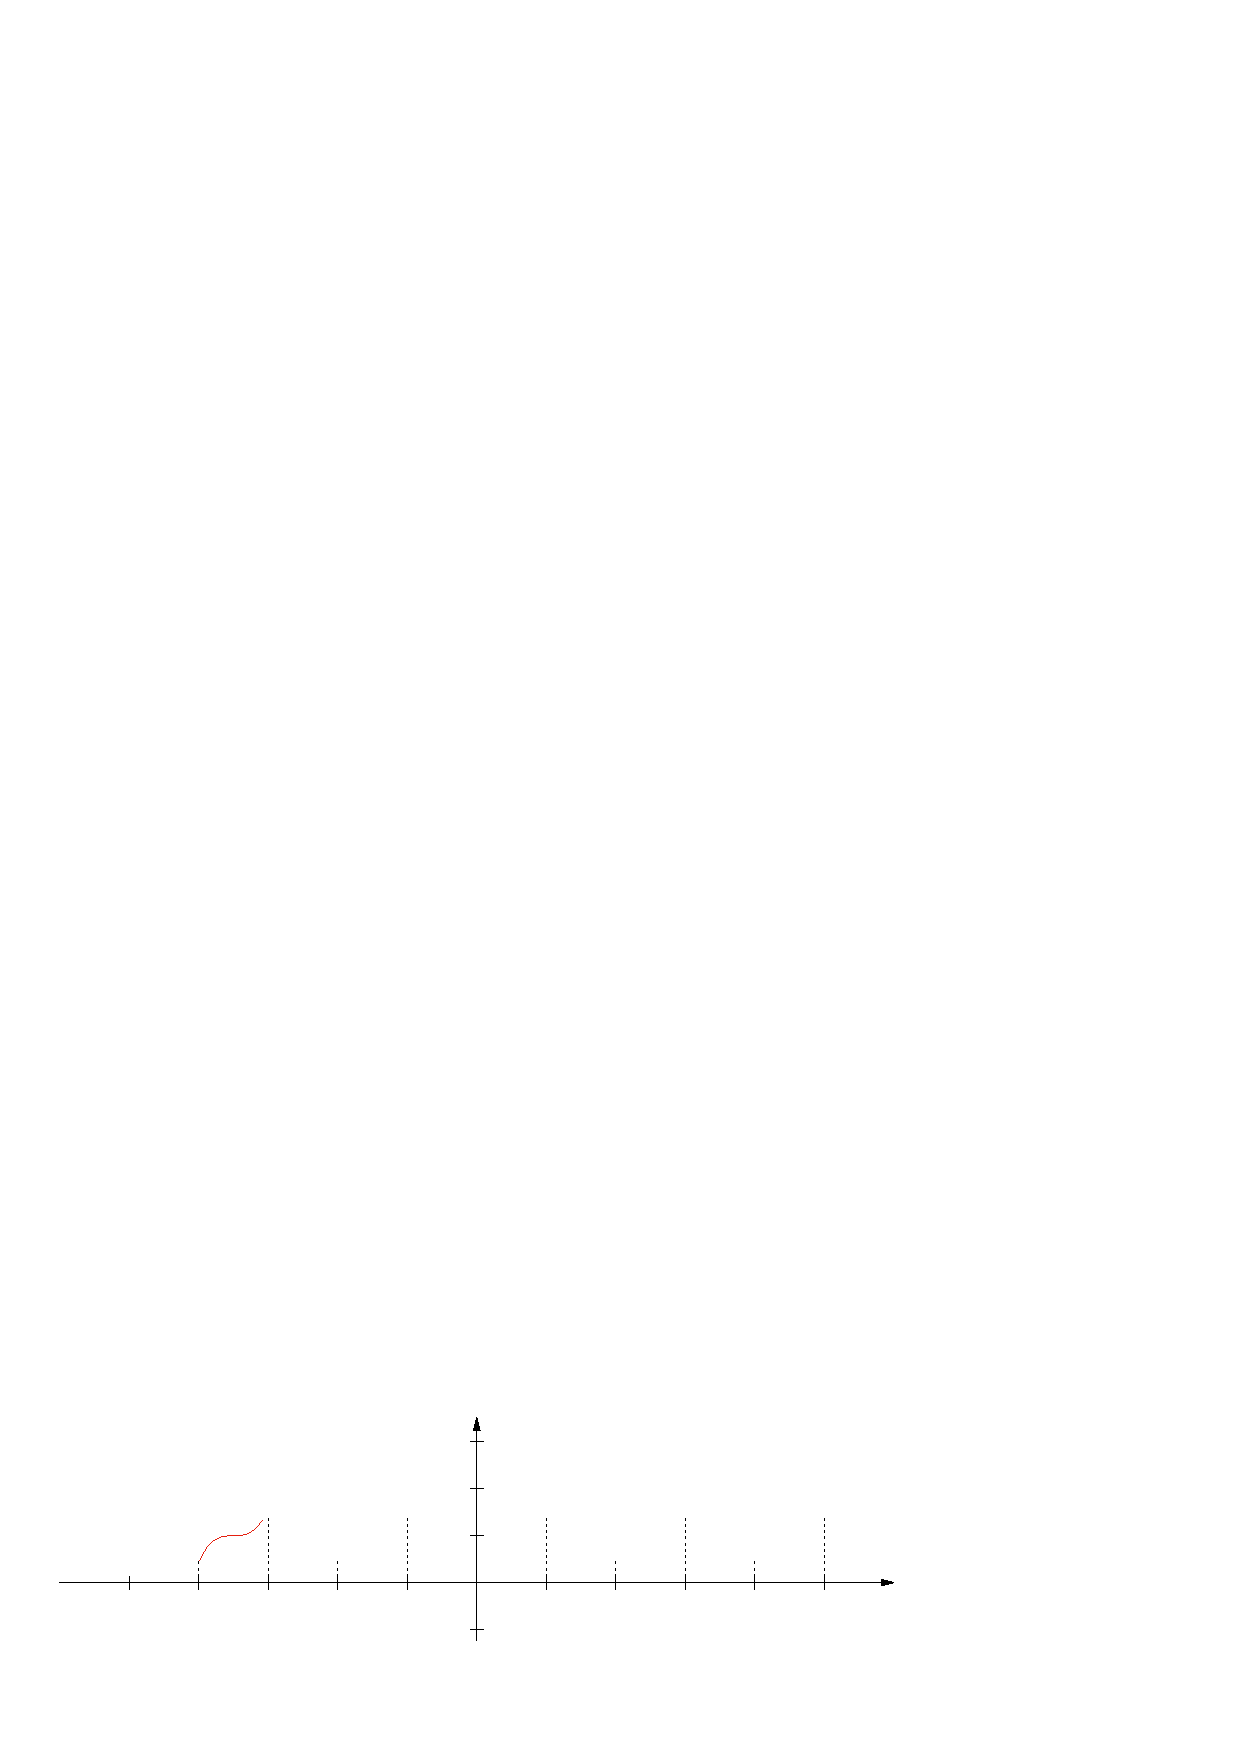
\includegraphics[width={360.00bp},height={108.00bp}]{figura_04_01}}%
    \gplfronttext
  \end{picture}%
\endgroup

\end{figure}

Cuando $f(t)$ es periódica tiene la siguiente representación (forma compleja):
\begin{equation*}
    f(t)=\sum_{n=-\infty}^\infty c_n\,e^{jn\omega_0 t}
\end{equation*}

Donde:
\begin{equation*}
    c_n=\frac{1}{T}\int_{-T/2}^{T/2} f(t)\,e^{-jn\omega_0 t}\,dt
\end{equation*}

Si $T\to\infty$, entonces $\omega_0\to0$, y la función deja de ser periódica.
\begin{equation*}
    f(t)=\sum_{n=-\infty}^\infty\left[
        \frac{1}{T}\int_{-T/2}^{T/2} f(\tau)\,e^{-jn\omega_0 \tau}\,d\tau
    \right]\,e^{jn\omega_0 t}
\end{equation*}
\begin{equation*}
    \frac{1}{T}=\frac{\omega_0}{2\pi}
\end{equation*}
\begin{equation*}
    f(t)=\frac{1}{2\pi}\sum_{n=-\infty}^\infty\left[
        \int_{-T/2}^{T/2} f(\tau)\,e^{-jn\omega_0 \tau}\,d\tau
    \right]\,e^{jn\omega_0 t}\,\omega_0
\end{equation*}
\begin{equation*}
    \omega_0=d\omega
\end{equation*}
\begin{equation*}
    n\omega_0=\omega
\end{equation*}
\begin{equation}
    f(t)=\frac{1}{2\pi}\int_{-\infty}^\infty\left[
        \int_{-\infty}^{\infty} f(\tau)\,e^{-j\omega\tau}\,d\tau
    \right]\,e^{j\omega t}\,d\omega
\end{equation}

Se define como transformada de \emph{Fourier}:
\begin{equation}
    F(\omega)=\int_{-\infty}^{\infty} f(t)\,e^{-j\omega t}\,dt
\end{equation}

Se define como transformada inversa de \emph{Fourier}:
\begin{equation}
    f(t)=\frac{1}{2\pi}\int_{-\infty}^\infty F(\omega)\,e^{j\omega t}\,d\omega
\end{equation}

\section{Transformada de \emph{Fourier}}
Dada una función $f(t)$ se define la transformada de \emph{Fourier}:
\begin{equation}
    \mathcal{F}\{f(t)\}=F(\omega)
        =\int_{-\infty}^{\infty} f(t)\,e^{-j\omega t}\,dt
\end{equation}

Donde: $f(t)$ es una función no periódica.

La transformada de \emph{Fourier} convierte una función del dominio del tiempo
($t$) al dominio de la frecuencia ($\omega$) la cual será una variable continua.

Para $f(t)\in\mathbb{R}$:
\begin{equation*}
\begin{split}
    F(\omega)
        &=\int_{-\infty}^{\infty} f(t)\,e^{-j\omega t}\,dt\\
        &=\int_{-\infty}^{\infty} f(t)[\cos(\omega t)-j\sen(\omega t)]\,dt\\
        &=\int_{-\infty}^{\infty} f(t)\cos(\omega t)\,dt
            -j\int_{-\infty}^{\infty} f(t)\sen(\omega t)\,dt\\
        &=R(\omega)+jX(\omega)\\
\end{split}
\end{equation*}
\begin{equation*}
    R(\omega)=\int_{-\infty}^{\infty} f(t)\cos(\omega t)\,dt
\end{equation*}
\begin{equation*}
    X(\omega)=-\int_{-\infty}^{\infty} f(t)\sen(\omega t)\,dt\\
\end{equation*}

La parte real $R(\omega)$ es una función par:
\begin{equation*}
    R(-\omega)=R(\omega)
\end{equation*}

La parte imaginaria $X(\omega)$ es una función impar:
\begin{equation*}
    X(-\omega)=-X(\omega)
\end{equation*}

Por tanto:

Si $f(t)$ es par, entonces $X(\omega)=0$.

Si $f(t)$ es impar, entonces $R(\omega)=0$.

\section{Espectros continuos de frecuencia}
\begin{equation*}
    F(\omega)=R(\omega)+jX(\omega)
\end{equation*}

Modulo:
\begin{equation*}
    |F(\omega)|=\sqrt{R^2(\omega)+X^2(\omega)}
\end{equation*}

Argumento:
\begin{equation*}
    \theta(\omega)=\arctan\left(\frac{X(\omega)}{R(\omega)}\right)
\end{equation*}

\textbf{Ejemplo 1:} Hallar $F(\omega)$ de la función y graficar los espectros.
\begin{equation*}
    f(t)=u(t+a)-u(t-a)
\end{equation*}
\begin{figure}[H]
    \centering
    % GNUPLOT: LaTeX picture with Postscript
\begingroup
  \makeatletter
  \providecommand\color[2][]{%
    \GenericError{(gnuplot) \space\space\space\@spaces}{%
      Package color not loaded in conjunction with
      terminal option `colourtext'%
    }{See the gnuplot documentation for explanation.%
    }{Either use 'blacktext' in gnuplot or load the package
      color.sty in LaTeX.}%
    \renewcommand\color[2][]{}%
  }%
  \providecommand\includegraphics[2][]{%
    \GenericError{(gnuplot) \space\space\space\@spaces}{%
      Package graphicx or graphics not loaded%
    }{See the gnuplot documentation for explanation.%
    }{The gnuplot epslatex terminal needs graphicx.sty or graphics.sty.}%
    \renewcommand\includegraphics[2][]{}%
  }%
  \providecommand\rotatebox[2]{#2}%
  \@ifundefined{ifGPcolor}{%
    \newif\ifGPcolor
    \GPcolorfalse
  }{}%
  \@ifundefined{ifGPblacktext}{%
    \newif\ifGPblacktext
    \GPblacktexttrue
  }{}%
  % define a \g@addto@macro without @ in the name:
  \let\gplgaddtomacro\g@addto@macro
  % define empty templates for all commands taking text:
  \gdef\gplbacktext{}%
  \gdef\gplfronttext{}%
  \makeatother
  \ifGPblacktext
    % no textcolor at all
    \def\colorrgb#1{}%
    \def\colorgray#1{}%
  \else
    % gray or color?
    \ifGPcolor
      \def\colorrgb#1{\color[rgb]{#1}}%
      \def\colorgray#1{\color[gray]{#1}}%
      \expandafter\def\csname LTw\endcsname{\color{white}}%
      \expandafter\def\csname LTb\endcsname{\color{black}}%
      \expandafter\def\csname LTa\endcsname{\color{black}}%
      \expandafter\def\csname LT0\endcsname{\color[rgb]{1,0,0}}%
      \expandafter\def\csname LT1\endcsname{\color[rgb]{0,1,0}}%
      \expandafter\def\csname LT2\endcsname{\color[rgb]{0,0,1}}%
      \expandafter\def\csname LT3\endcsname{\color[rgb]{1,0,1}}%
      \expandafter\def\csname LT4\endcsname{\color[rgb]{0,1,1}}%
      \expandafter\def\csname LT5\endcsname{\color[rgb]{1,1,0}}%
      \expandafter\def\csname LT6\endcsname{\color[rgb]{0,0,0}}%
      \expandafter\def\csname LT7\endcsname{\color[rgb]{1,0.3,0}}%
      \expandafter\def\csname LT8\endcsname{\color[rgb]{0.5,0.5,0.5}}%
    \else
      % gray
      \def\colorrgb#1{\color{black}}%
      \def\colorgray#1{\color[gray]{#1}}%
      \expandafter\def\csname LTw\endcsname{\color{white}}%
      \expandafter\def\csname LTb\endcsname{\color{black}}%
      \expandafter\def\csname LTa\endcsname{\color{black}}%
      \expandafter\def\csname LT0\endcsname{\color{black}}%
      \expandafter\def\csname LT1\endcsname{\color{black}}%
      \expandafter\def\csname LT2\endcsname{\color{black}}%
      \expandafter\def\csname LT3\endcsname{\color{black}}%
      \expandafter\def\csname LT4\endcsname{\color{black}}%
      \expandafter\def\csname LT5\endcsname{\color{black}}%
      \expandafter\def\csname LT6\endcsname{\color{black}}%
      \expandafter\def\csname LT7\endcsname{\color{black}}%
      \expandafter\def\csname LT8\endcsname{\color{black}}%
    \fi
  \fi
    \setlength{\unitlength}{0.0500bp}%
    \ifx\gptboxheight\undefined%
      \newlength{\gptboxheight}%
      \newlength{\gptboxwidth}%
      \newsavebox{\gptboxtext}%
    \fi%
    \setlength{\fboxrule}{0.5pt}%
    \setlength{\fboxsep}{1pt}%
    \definecolor{tbcol}{rgb}{1,1,1}%
\begin{picture}(2160.00,1728.00)%
    \gplgaddtomacro\gplbacktext{%
      \csname LTb\endcsname%%
      \put(960,192){\makebox(0,0)[r]{\strut{}}}%
      \put(960,650){\makebox(0,0)[r]{\strut{}}}%
      \put(960,1109){\makebox(0,0)[r]{\strut{}}}%
      \put(960,1567){\makebox(0,0)[r]{\strut{}}}%
      \put(240,427){\makebox(0,0){\strut{}}}%
      \put(648,427){\makebox(0,0){\strut{}}}%
      \put(1056,427){\makebox(0,0){\strut{}}}%
      \put(1463,427){\makebox(0,0){\strut{}}}%
      \put(1871,427){\makebox(0,0){\strut{}}}%
      \csname LTb\endcsname%%
      \put(2279,650){\makebox(0,0)[l]{\strut{}$t$}}%
      \put(1239,1750){\makebox(0,0)[l]{\strut{}$f(t)$}}%
      \put(1422,375){\makebox(0,0)[l]{\strut{}$ a$}}%
      \put(444,375){\makebox(0,0)[l]{\strut{}$-a$}}%
      \put(852,1292){\makebox(0,0)[l]{\strut{}$1$}}%
    }%
    \gplgaddtomacro\gplfronttext{%
    }%
    \gplbacktext
    \put(0,0){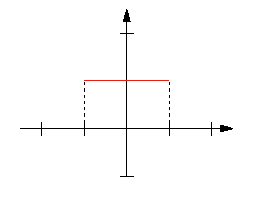
\includegraphics[width={108.00bp},height={86.40bp}]{figura_04_02}}%
    \gplfronttext
  \end{picture}%
\endgroup

\end{figure}
\begin{equation*}
\begin{split}
    F(\omega)
        &=\int_{-a}^a 1\,e^{-j\omega t}\,dt\\
        &=\frac{e^{-j\omega t}}{-j\omega}\Biggr|_{-a}^a\\
        &=\frac{e^{-ja\omega}-e^{ja\omega}}{-j\omega}\\
        &=\frac{-2j\sen(a\omega)}{-j\omega}\\
        &=\frac{2\sen(a\omega)}{\omega}\\
\end{split}
\end{equation*}
\begin{equation}
    \mathcal{F}\{u(t+a)-u(t-a)\}=\frac{2\sen(a\omega)}{\omega}
\end{equation}
\begin{equation*}
    |F(\omega)|=|\frac{2\sen(a\omega)}{\omega}|
\end{equation*}

Para $\omega=0$, existe una discontinuidad:
\begin{equation*}
    \lim_{\omega\to0}\left(\frac{2\sen(a\omega)}{\omega}\right)=2a
\end{equation*}
\begin{figure}[H]
    \centering
    \begin{minipage}{.4\textwidth}
        \centering
        % GNUPLOT: LaTeX picture with Postscript
\begingroup
  \makeatletter
  \providecommand\color[2][]{%
    \GenericError{(gnuplot) \space\space\space\@spaces}{%
      Package color not loaded in conjunction with
      terminal option `colourtext'%
    }{See the gnuplot documentation for explanation.%
    }{Either use 'blacktext' in gnuplot or load the package
      color.sty in LaTeX.}%
    \renewcommand\color[2][]{}%
  }%
  \providecommand\includegraphics[2][]{%
    \GenericError{(gnuplot) \space\space\space\@spaces}{%
      Package graphicx or graphics not loaded%
    }{See the gnuplot documentation for explanation.%
    }{The gnuplot epslatex terminal needs graphicx.sty or graphics.sty.}%
    \renewcommand\includegraphics[2][]{}%
  }%
  \providecommand\rotatebox[2]{#2}%
  \@ifundefined{ifGPcolor}{%
    \newif\ifGPcolor
    \GPcolorfalse
  }{}%
  \@ifundefined{ifGPblacktext}{%
    \newif\ifGPblacktext
    \GPblacktexttrue
  }{}%
  % define a \g@addto@macro without @ in the name:
  \let\gplgaddtomacro\g@addto@macro
  % define empty templates for all commands taking text:
  \gdef\gplbacktext{}%
  \gdef\gplfronttext{}%
  \makeatother
  \ifGPblacktext
    % no textcolor at all
    \def\colorrgb#1{}%
    \def\colorgray#1{}%
  \else
    % gray or color?
    \ifGPcolor
      \def\colorrgb#1{\color[rgb]{#1}}%
      \def\colorgray#1{\color[gray]{#1}}%
      \expandafter\def\csname LTw\endcsname{\color{white}}%
      \expandafter\def\csname LTb\endcsname{\color{black}}%
      \expandafter\def\csname LTa\endcsname{\color{black}}%
      \expandafter\def\csname LT0\endcsname{\color[rgb]{1,0,0}}%
      \expandafter\def\csname LT1\endcsname{\color[rgb]{0,1,0}}%
      \expandafter\def\csname LT2\endcsname{\color[rgb]{0,0,1}}%
      \expandafter\def\csname LT3\endcsname{\color[rgb]{1,0,1}}%
      \expandafter\def\csname LT4\endcsname{\color[rgb]{0,1,1}}%
      \expandafter\def\csname LT5\endcsname{\color[rgb]{1,1,0}}%
      \expandafter\def\csname LT6\endcsname{\color[rgb]{0,0,0}}%
      \expandafter\def\csname LT7\endcsname{\color[rgb]{1,0.3,0}}%
      \expandafter\def\csname LT8\endcsname{\color[rgb]{0.5,0.5,0.5}}%
    \else
      % gray
      \def\colorrgb#1{\color{black}}%
      \def\colorgray#1{\color[gray]{#1}}%
      \expandafter\def\csname LTw\endcsname{\color{white}}%
      \expandafter\def\csname LTb\endcsname{\color{black}}%
      \expandafter\def\csname LTa\endcsname{\color{black}}%
      \expandafter\def\csname LT0\endcsname{\color{black}}%
      \expandafter\def\csname LT1\endcsname{\color{black}}%
      \expandafter\def\csname LT2\endcsname{\color{black}}%
      \expandafter\def\csname LT3\endcsname{\color{black}}%
      \expandafter\def\csname LT4\endcsname{\color{black}}%
      \expandafter\def\csname LT5\endcsname{\color{black}}%
      \expandafter\def\csname LT6\endcsname{\color{black}}%
      \expandafter\def\csname LT7\endcsname{\color{black}}%
      \expandafter\def\csname LT8\endcsname{\color{black}}%
    \fi
  \fi
    \setlength{\unitlength}{0.0500bp}%
    \ifx\gptboxheight\undefined%
      \newlength{\gptboxheight}%
      \newlength{\gptboxwidth}%
      \newsavebox{\gptboxtext}%
    \fi%
    \setlength{\fboxrule}{0.5pt}%
    \setlength{\fboxsep}{1pt}%
    \definecolor{tbcol}{rgb}{1,1,1}%
\begin{picture}(3168.00,2160.00)%
    \gplgaddtomacro\gplbacktext{%
      \csname LTb\endcsname%%
      \put(1464,644){\makebox(0,0)[r]{\strut{}}}%
      \put(1464,1547){\makebox(0,0)[r]{\strut{}}}%
      \put(240,421){\makebox(0,0){\strut{}}}%
      \put(570,421){\makebox(0,0){\strut{}}}%
      \put(900,421){\makebox(0,0){\strut{}}}%
      \put(1230,421){\makebox(0,0){\strut{}}}%
      \put(1560,421){\makebox(0,0){\strut{}}}%
      \put(1889,421){\makebox(0,0){\strut{}}}%
      \put(2219,421){\makebox(0,0){\strut{}}}%
      \put(2549,421){\makebox(0,0){\strut{}}}%
      \put(2879,421){\makebox(0,0){\strut{}}}%
      \csname LTb\endcsname%%
      \put(3110,644){\makebox(0,0)[l]{\strut{}$\omega$}}%
      \put(751,2270){\makebox(0,0)[l]{\strut{}$|F(\omega)|$}}%
    }%
    \gplgaddtomacro\gplfronttext{%
    }%
    \gplbacktext
    \put(0,0){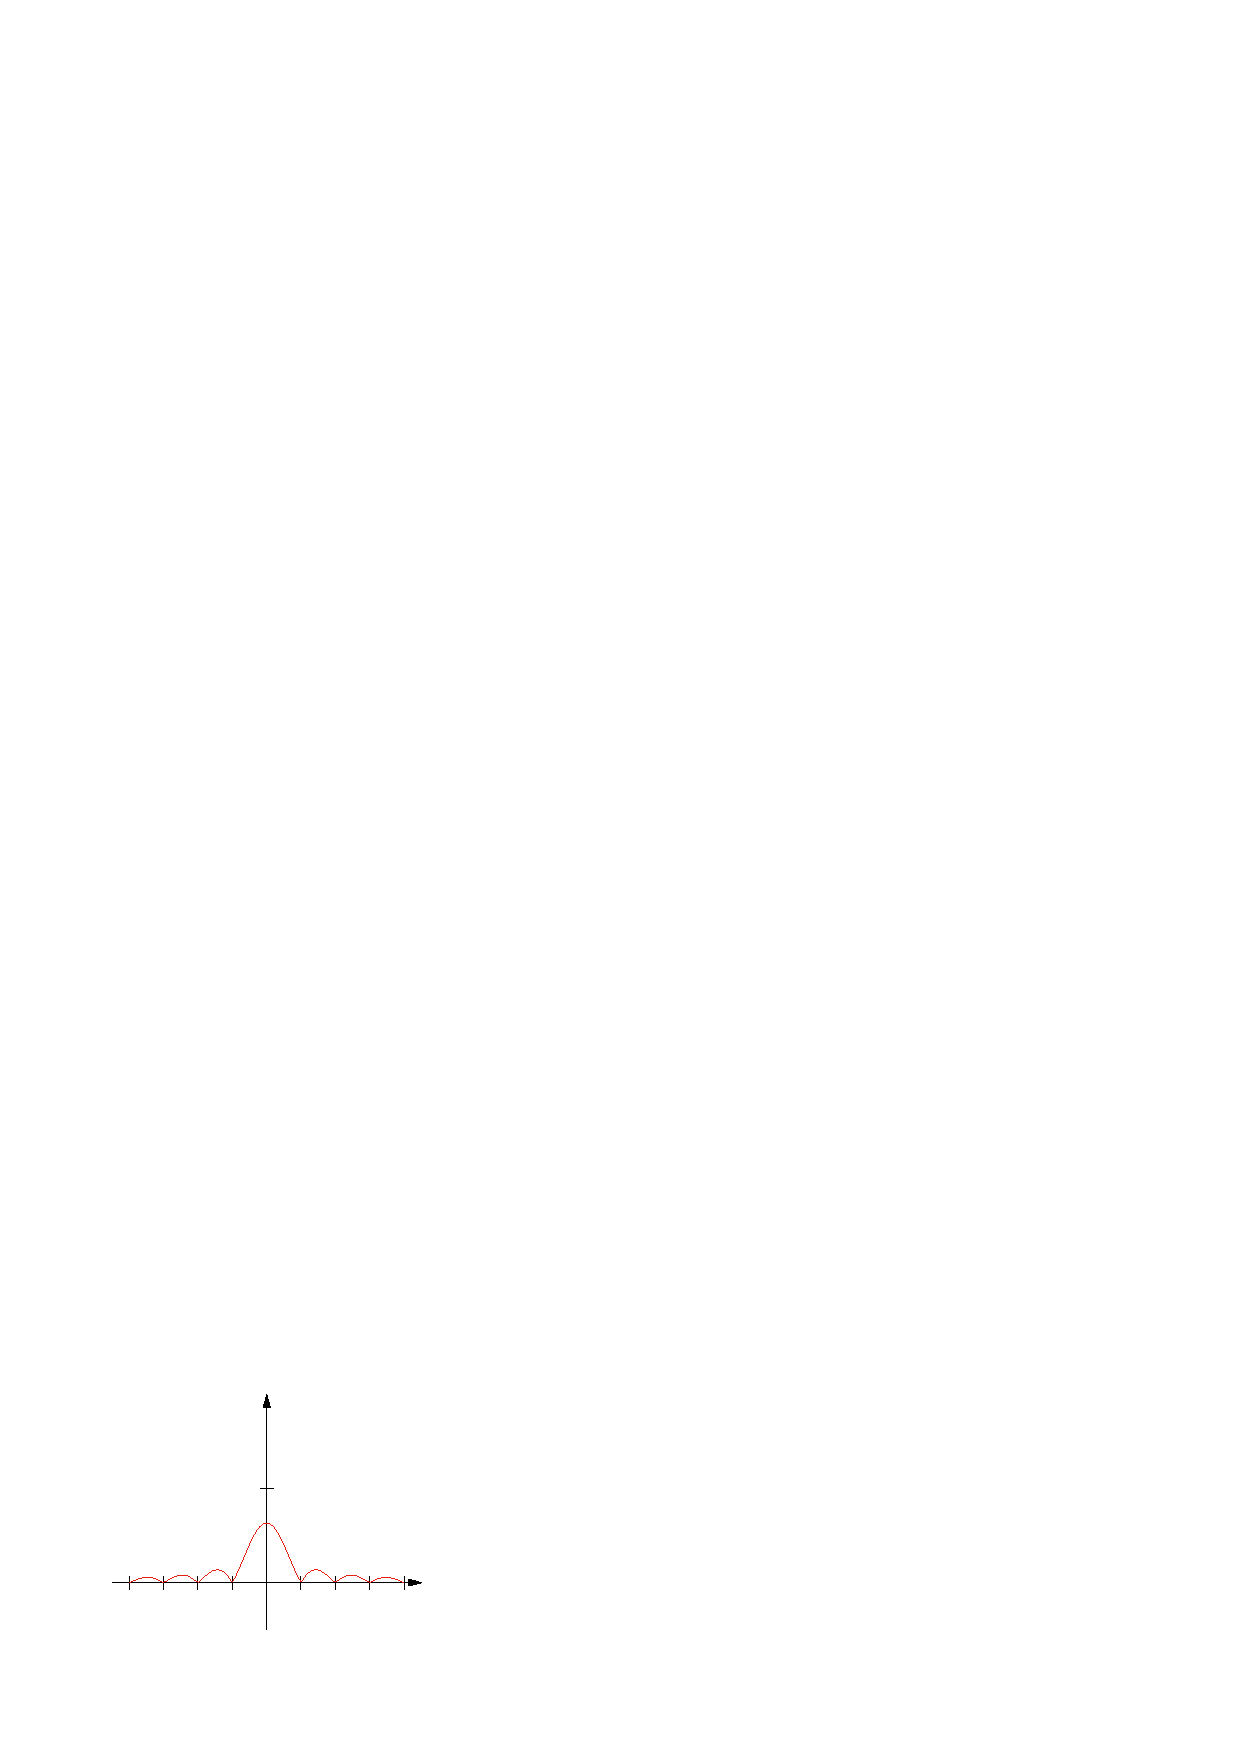
\includegraphics[width={158.40bp},height={108.00bp}]{figura_04_03}}%
    \gplfronttext
  \end{picture}%
\endgroup

    \end{minipage}
    \begin{minipage}{.4\textwidth}
        \centering
        % GNUPLOT: LaTeX picture with Postscript
\begingroup
  \makeatletter
  \providecommand\color[2][]{%
    \GenericError{(gnuplot) \space\space\space\@spaces}{%
      Package color not loaded in conjunction with
      terminal option `colourtext'%
    }{See the gnuplot documentation for explanation.%
    }{Either use 'blacktext' in gnuplot or load the package
      color.sty in LaTeX.}%
    \renewcommand\color[2][]{}%
  }%
  \providecommand\includegraphics[2][]{%
    \GenericError{(gnuplot) \space\space\space\@spaces}{%
      Package graphicx or graphics not loaded%
    }{See the gnuplot documentation for explanation.%
    }{The gnuplot epslatex terminal needs graphicx.sty or graphics.sty.}%
    \renewcommand\includegraphics[2][]{}%
  }%
  \providecommand\rotatebox[2]{#2}%
  \@ifundefined{ifGPcolor}{%
    \newif\ifGPcolor
    \GPcolorfalse
  }{}%
  \@ifundefined{ifGPblacktext}{%
    \newif\ifGPblacktext
    \GPblacktexttrue
  }{}%
  % define a \g@addto@macro without @ in the name:
  \let\gplgaddtomacro\g@addto@macro
  % define empty templates for all commands taking text:
  \gdef\gplbacktext{}%
  \gdef\gplfronttext{}%
  \makeatother
  \ifGPblacktext
    % no textcolor at all
    \def\colorrgb#1{}%
    \def\colorgray#1{}%
  \else
    % gray or color?
    \ifGPcolor
      \def\colorrgb#1{\color[rgb]{#1}}%
      \def\colorgray#1{\color[gray]{#1}}%
      \expandafter\def\csname LTw\endcsname{\color{white}}%
      \expandafter\def\csname LTb\endcsname{\color{black}}%
      \expandafter\def\csname LTa\endcsname{\color{black}}%
      \expandafter\def\csname LT0\endcsname{\color[rgb]{1,0,0}}%
      \expandafter\def\csname LT1\endcsname{\color[rgb]{0,1,0}}%
      \expandafter\def\csname LT2\endcsname{\color[rgb]{0,0,1}}%
      \expandafter\def\csname LT3\endcsname{\color[rgb]{1,0,1}}%
      \expandafter\def\csname LT4\endcsname{\color[rgb]{0,1,1}}%
      \expandafter\def\csname LT5\endcsname{\color[rgb]{1,1,0}}%
      \expandafter\def\csname LT6\endcsname{\color[rgb]{0,0,0}}%
      \expandafter\def\csname LT7\endcsname{\color[rgb]{1,0.3,0}}%
      \expandafter\def\csname LT8\endcsname{\color[rgb]{0.5,0.5,0.5}}%
    \else
      % gray
      \def\colorrgb#1{\color{black}}%
      \def\colorgray#1{\color[gray]{#1}}%
      \expandafter\def\csname LTw\endcsname{\color{white}}%
      \expandafter\def\csname LTb\endcsname{\color{black}}%
      \expandafter\def\csname LTa\endcsname{\color{black}}%
      \expandafter\def\csname LT0\endcsname{\color{black}}%
      \expandafter\def\csname LT1\endcsname{\color{black}}%
      \expandafter\def\csname LT2\endcsname{\color{black}}%
      \expandafter\def\csname LT3\endcsname{\color{black}}%
      \expandafter\def\csname LT4\endcsname{\color{black}}%
      \expandafter\def\csname LT5\endcsname{\color{black}}%
      \expandafter\def\csname LT6\endcsname{\color{black}}%
      \expandafter\def\csname LT7\endcsname{\color{black}}%
      \expandafter\def\csname LT8\endcsname{\color{black}}%
    \fi
  \fi
    \setlength{\unitlength}{0.0500bp}%
    \ifx\gptboxheight\undefined%
      \newlength{\gptboxheight}%
      \newlength{\gptboxwidth}%
      \newsavebox{\gptboxtext}%
    \fi%
    \setlength{\fboxrule}{0.5pt}%
    \setlength{\fboxsep}{1pt}%
    \definecolor{tbcol}{rgb}{1,1,1}%
\begin{picture}(3168.00,2160.00)%
    \gplgaddtomacro\gplbacktext{%
      \csname LTb\endcsname%%
      \put(1464,644){\makebox(0,0)[r]{\strut{}}}%
      \put(1464,1547){\makebox(0,0)[r]{\strut{}}}%
      \put(240,421){\makebox(0,0){\strut{}}}%
      \put(570,421){\makebox(0,0){\strut{}}}%
      \put(900,421){\makebox(0,0){\strut{}}}%
      \put(1230,421){\makebox(0,0){\strut{}}}%
      \put(1560,421){\makebox(0,0){\strut{}}}%
      \put(1889,421){\makebox(0,0){\strut{}}}%
      \put(2219,421){\makebox(0,0){\strut{}}}%
      \put(2549,421){\makebox(0,0){\strut{}}}%
      \put(2879,421){\makebox(0,0){\strut{}}}%
      \csname LTb\endcsname%%
      \put(3110,644){\makebox(0,0)[l]{\strut{}$\omega$}}%
      \put(982,2270){\makebox(0,0)[l]{\strut{}$\theta(\omega)$}}%
    }%
    \gplgaddtomacro\gplfronttext{%
    }%
    \gplgaddtomacro\gplbacktext{%
      \csname LTb\endcsname%%
      \put(1464,644){\makebox(0,0)[r]{\strut{}}}%
      \put(1464,1547){\makebox(0,0)[r]{\strut{}}}%
      \put(240,421){\makebox(0,0){\strut{}}}%
      \put(570,421){\makebox(0,0){\strut{}}}%
      \put(900,421){\makebox(0,0){\strut{}}}%
      \put(1230,421){\makebox(0,0){\strut{}}}%
      \put(1560,421){\makebox(0,0){\strut{}}}%
      \put(1889,421){\makebox(0,0){\strut{}}}%
      \put(2219,421){\makebox(0,0){\strut{}}}%
      \put(2549,421){\makebox(0,0){\strut{}}}%
      \put(2879,421){\makebox(0,0){\strut{}}}%
      \csname LTb\endcsname%%
      \put(3110,644){\makebox(0,0)[l]{\strut{}$\omega$}}%
      \put(982,2270){\makebox(0,0)[l]{\strut{}$\theta(\omega)$}}%
    }%
    \gplgaddtomacro\gplfronttext{%
    }%
    \gplgaddtomacro\gplbacktext{%
      \csname LTb\endcsname%%
      \put(1464,644){\makebox(0,0)[r]{\strut{}}}%
      \put(1464,1547){\makebox(0,0)[r]{\strut{}}}%
      \put(240,421){\makebox(0,0){\strut{}}}%
      \put(570,421){\makebox(0,0){\strut{}}}%
      \put(900,421){\makebox(0,0){\strut{}}}%
      \put(1230,421){\makebox(0,0){\strut{}}}%
      \put(1560,421){\makebox(0,0){\strut{}}}%
      \put(1889,421){\makebox(0,0){\strut{}}}%
      \put(2219,421){\makebox(0,0){\strut{}}}%
      \put(2549,421){\makebox(0,0){\strut{}}}%
      \put(2879,421){\makebox(0,0){\strut{}}}%
      \csname LTb\endcsname%%
      \put(3110,644){\makebox(0,0)[l]{\strut{}$\omega$}}%
      \put(982,2270){\makebox(0,0)[l]{\strut{}$\theta(\omega)$}}%
    }%
    \gplgaddtomacro\gplfronttext{%
    }%
    \gplgaddtomacro\gplbacktext{%
      \csname LTb\endcsname%%
      \put(1464,644){\makebox(0,0)[r]{\strut{}}}%
      \put(1464,1547){\makebox(0,0)[r]{\strut{}}}%
      \put(240,421){\makebox(0,0){\strut{}}}%
      \put(570,421){\makebox(0,0){\strut{}}}%
      \put(900,421){\makebox(0,0){\strut{}}}%
      \put(1230,421){\makebox(0,0){\strut{}}}%
      \put(1560,421){\makebox(0,0){\strut{}}}%
      \put(1889,421){\makebox(0,0){\strut{}}}%
      \put(2219,421){\makebox(0,0){\strut{}}}%
      \put(2549,421){\makebox(0,0){\strut{}}}%
      \put(2879,421){\makebox(0,0){\strut{}}}%
      \csname LTb\endcsname%%
      \put(3110,644){\makebox(0,0)[l]{\strut{}$\omega$}}%
      \put(982,2270){\makebox(0,0)[l]{\strut{}$\theta(\omega)$}}%
    }%
    \gplgaddtomacro\gplfronttext{%
    }%
    \gplgaddtomacro\gplbacktext{%
      \csname LTb\endcsname%%
      \put(1464,644){\makebox(0,0)[r]{\strut{}}}%
      \put(1464,1547){\makebox(0,0)[r]{\strut{}}}%
      \put(240,421){\makebox(0,0){\strut{}}}%
      \put(570,421){\makebox(0,0){\strut{}}}%
      \put(900,421){\makebox(0,0){\strut{}}}%
      \put(1230,421){\makebox(0,0){\strut{}}}%
      \put(1560,421){\makebox(0,0){\strut{}}}%
      \put(1889,421){\makebox(0,0){\strut{}}}%
      \put(2219,421){\makebox(0,0){\strut{}}}%
      \put(2549,421){\makebox(0,0){\strut{}}}%
      \put(2879,421){\makebox(0,0){\strut{}}}%
      \csname LTb\endcsname%%
      \put(3110,644){\makebox(0,0)[l]{\strut{}$\omega$}}%
      \put(982,2270){\makebox(0,0)[l]{\strut{}$\theta(\omega)$}}%
    }%
    \gplgaddtomacro\gplfronttext{%
    }%
    \gplgaddtomacro\gplbacktext{%
      \csname LTb\endcsname%%
      \put(1464,644){\makebox(0,0)[r]{\strut{}}}%
      \put(1464,1547){\makebox(0,0)[r]{\strut{}}}%
      \put(240,421){\makebox(0,0){\strut{}}}%
      \put(570,421){\makebox(0,0){\strut{}}}%
      \put(900,421){\makebox(0,0){\strut{}}}%
      \put(1230,421){\makebox(0,0){\strut{}}}%
      \put(1560,421){\makebox(0,0){\strut{}}}%
      \put(1889,421){\makebox(0,0){\strut{}}}%
      \put(2219,421){\makebox(0,0){\strut{}}}%
      \put(2549,421){\makebox(0,0){\strut{}}}%
      \put(2879,421){\makebox(0,0){\strut{}}}%
      \csname LTb\endcsname%%
      \put(3110,644){\makebox(0,0)[l]{\strut{}$\omega$}}%
      \put(982,2270){\makebox(0,0)[l]{\strut{}$\theta(\omega)$}}%
    }%
    \gplgaddtomacro\gplfronttext{%
    }%
    \gplgaddtomacro\gplbacktext{%
      \csname LTb\endcsname%%
      \put(1464,644){\makebox(0,0)[r]{\strut{}}}%
      \put(1464,1547){\makebox(0,0)[r]{\strut{}}}%
      \put(240,421){\makebox(0,0){\strut{}}}%
      \put(570,421){\makebox(0,0){\strut{}}}%
      \put(900,421){\makebox(0,0){\strut{}}}%
      \put(1230,421){\makebox(0,0){\strut{}}}%
      \put(1560,421){\makebox(0,0){\strut{}}}%
      \put(1889,421){\makebox(0,0){\strut{}}}%
      \put(2219,421){\makebox(0,0){\strut{}}}%
      \put(2549,421){\makebox(0,0){\strut{}}}%
      \put(2879,421){\makebox(0,0){\strut{}}}%
      \csname LTb\endcsname%%
      \put(3110,644){\makebox(0,0)[l]{\strut{}$\omega$}}%
      \put(982,2270){\makebox(0,0)[l]{\strut{}$\theta(\omega)$}}%
    }%
    \gplgaddtomacro\gplfronttext{%
    }%
    \gplgaddtomacro\gplbacktext{%
      \csname LTb\endcsname%%
      \put(1464,644){\makebox(0,0)[r]{\strut{}}}%
      \put(1464,1547){\makebox(0,0)[r]{\strut{}}}%
      \put(240,421){\makebox(0,0){\strut{}}}%
      \put(570,421){\makebox(0,0){\strut{}}}%
      \put(900,421){\makebox(0,0){\strut{}}}%
      \put(1230,421){\makebox(0,0){\strut{}}}%
      \put(1560,421){\makebox(0,0){\strut{}}}%
      \put(1889,421){\makebox(0,0){\strut{}}}%
      \put(2219,421){\makebox(0,0){\strut{}}}%
      \put(2549,421){\makebox(0,0){\strut{}}}%
      \put(2879,421){\makebox(0,0){\strut{}}}%
      \csname LTb\endcsname%%
      \put(3110,644){\makebox(0,0)[l]{\strut{}$\omega$}}%
      \put(982,2270){\makebox(0,0)[l]{\strut{}$\theta(\omega)$}}%
    }%
    \gplgaddtomacro\gplfronttext{%
    }%
    \gplgaddtomacro\gplbacktext{%
      \csname LTb\endcsname%%
      \put(1464,644){\makebox(0,0)[r]{\strut{}}}%
      \put(1464,1547){\makebox(0,0)[r]{\strut{}}}%
      \put(240,421){\makebox(0,0){\strut{}}}%
      \put(570,421){\makebox(0,0){\strut{}}}%
      \put(900,421){\makebox(0,0){\strut{}}}%
      \put(1230,421){\makebox(0,0){\strut{}}}%
      \put(1560,421){\makebox(0,0){\strut{}}}%
      \put(1889,421){\makebox(0,0){\strut{}}}%
      \put(2219,421){\makebox(0,0){\strut{}}}%
      \put(2549,421){\makebox(0,0){\strut{}}}%
      \put(2879,421){\makebox(0,0){\strut{}}}%
      \csname LTb\endcsname%%
      \put(3110,644){\makebox(0,0)[l]{\strut{}$\omega$}}%
      \put(982,2270){\makebox(0,0)[l]{\strut{}$\theta(\omega)$}}%
    }%
    \gplgaddtomacro\gplfronttext{%
    }%
    \gplgaddtomacro\gplbacktext{%
      \csname LTb\endcsname%%
      \put(1464,644){\makebox(0,0)[r]{\strut{}}}%
      \put(1464,1547){\makebox(0,0)[r]{\strut{}}}%
      \put(240,421){\makebox(0,0){\strut{}}}%
      \put(570,421){\makebox(0,0){\strut{}}}%
      \put(900,421){\makebox(0,0){\strut{}}}%
      \put(1230,421){\makebox(0,0){\strut{}}}%
      \put(1560,421){\makebox(0,0){\strut{}}}%
      \put(1889,421){\makebox(0,0){\strut{}}}%
      \put(2219,421){\makebox(0,0){\strut{}}}%
      \put(2549,421){\makebox(0,0){\strut{}}}%
      \put(2879,421){\makebox(0,0){\strut{}}}%
      \csname LTb\endcsname%%
      \put(3110,644){\makebox(0,0)[l]{\strut{}$\omega$}}%
      \put(982,2270){\makebox(0,0)[l]{\strut{}$\theta(\omega)$}}%
    }%
    \gplgaddtomacro\gplfronttext{%
    }%
    \gplgaddtomacro\gplbacktext{%
      \csname LTb\endcsname%%
      \put(1464,644){\makebox(0,0)[r]{\strut{}}}%
      \put(1464,1547){\makebox(0,0)[r]{\strut{}}}%
      \put(240,421){\makebox(0,0){\strut{}}}%
      \put(570,421){\makebox(0,0){\strut{}}}%
      \put(900,421){\makebox(0,0){\strut{}}}%
      \put(1230,421){\makebox(0,0){\strut{}}}%
      \put(1560,421){\makebox(0,0){\strut{}}}%
      \put(1889,421){\makebox(0,0){\strut{}}}%
      \put(2219,421){\makebox(0,0){\strut{}}}%
      \put(2549,421){\makebox(0,0){\strut{}}}%
      \put(2879,421){\makebox(0,0){\strut{}}}%
      \csname LTb\endcsname%%
      \put(3110,644){\makebox(0,0)[l]{\strut{}$\omega$}}%
      \put(982,2270){\makebox(0,0)[l]{\strut{}$\theta(\omega)$}}%
    }%
    \gplgaddtomacro\gplfronttext{%
    }%
    \gplgaddtomacro\gplbacktext{%
      \csname LTb\endcsname%%
      \put(1464,644){\makebox(0,0)[r]{\strut{}}}%
      \put(1464,1547){\makebox(0,0)[r]{\strut{}}}%
      \put(240,421){\makebox(0,0){\strut{}}}%
      \put(570,421){\makebox(0,0){\strut{}}}%
      \put(900,421){\makebox(0,0){\strut{}}}%
      \put(1230,421){\makebox(0,0){\strut{}}}%
      \put(1560,421){\makebox(0,0){\strut{}}}%
      \put(1889,421){\makebox(0,0){\strut{}}}%
      \put(2219,421){\makebox(0,0){\strut{}}}%
      \put(2549,421){\makebox(0,0){\strut{}}}%
      \put(2879,421){\makebox(0,0){\strut{}}}%
      \csname LTb\endcsname%%
      \put(3110,644){\makebox(0,0)[l]{\strut{}$\omega$}}%
      \put(982,2270){\makebox(0,0)[l]{\strut{}$\theta(\omega)$}}%
    }%
    \gplgaddtomacro\gplfronttext{%
    }%
    \gplgaddtomacro\gplbacktext{%
      \csname LTb\endcsname%%
      \put(1464,644){\makebox(0,0)[r]{\strut{}}}%
      \put(1464,1547){\makebox(0,0)[r]{\strut{}}}%
      \put(240,421){\makebox(0,0){\strut{}}}%
      \put(570,421){\makebox(0,0){\strut{}}}%
      \put(900,421){\makebox(0,0){\strut{}}}%
      \put(1230,421){\makebox(0,0){\strut{}}}%
      \put(1560,421){\makebox(0,0){\strut{}}}%
      \put(1889,421){\makebox(0,0){\strut{}}}%
      \put(2219,421){\makebox(0,0){\strut{}}}%
      \put(2549,421){\makebox(0,0){\strut{}}}%
      \put(2879,421){\makebox(0,0){\strut{}}}%
      \csname LTb\endcsname%%
      \put(3110,644){\makebox(0,0)[l]{\strut{}$\omega$}}%
      \put(982,2270){\makebox(0,0)[l]{\strut{}$\theta(\omega)$}}%
    }%
    \gplgaddtomacro\gplfronttext{%
    }%
    \gplgaddtomacro\gplbacktext{%
      \csname LTb\endcsname%%
      \put(1464,644){\makebox(0,0)[r]{\strut{}}}%
      \put(1464,1547){\makebox(0,0)[r]{\strut{}}}%
      \put(240,421){\makebox(0,0){\strut{}}}%
      \put(570,421){\makebox(0,0){\strut{}}}%
      \put(900,421){\makebox(0,0){\strut{}}}%
      \put(1230,421){\makebox(0,0){\strut{}}}%
      \put(1560,421){\makebox(0,0){\strut{}}}%
      \put(1889,421){\makebox(0,0){\strut{}}}%
      \put(2219,421){\makebox(0,0){\strut{}}}%
      \put(2549,421){\makebox(0,0){\strut{}}}%
      \put(2879,421){\makebox(0,0){\strut{}}}%
      \csname LTb\endcsname%%
      \put(3110,644){\makebox(0,0)[l]{\strut{}$\omega$}}%
      \put(982,2270){\makebox(0,0)[l]{\strut{}$\theta(\omega)$}}%
    }%
    \gplgaddtomacro\gplfronttext{%
    }%
    \gplgaddtomacro\gplbacktext{%
      \csname LTb\endcsname%%
      \put(1464,644){\makebox(0,0)[r]{\strut{}}}%
      \put(1464,1547){\makebox(0,0)[r]{\strut{}}}%
      \put(240,421){\makebox(0,0){\strut{}}}%
      \put(570,421){\makebox(0,0){\strut{}}}%
      \put(900,421){\makebox(0,0){\strut{}}}%
      \put(1230,421){\makebox(0,0){\strut{}}}%
      \put(1560,421){\makebox(0,0){\strut{}}}%
      \put(1889,421){\makebox(0,0){\strut{}}}%
      \put(2219,421){\makebox(0,0){\strut{}}}%
      \put(2549,421){\makebox(0,0){\strut{}}}%
      \put(2879,421){\makebox(0,0){\strut{}}}%
      \csname LTb\endcsname%%
      \put(3110,644){\makebox(0,0)[l]{\strut{}$\omega$}}%
      \put(982,2270){\makebox(0,0)[l]{\strut{}$\theta(\omega)$}}%
    }%
    \gplgaddtomacro\gplfronttext{%
    }%
    \gplbacktext
    \put(0,0){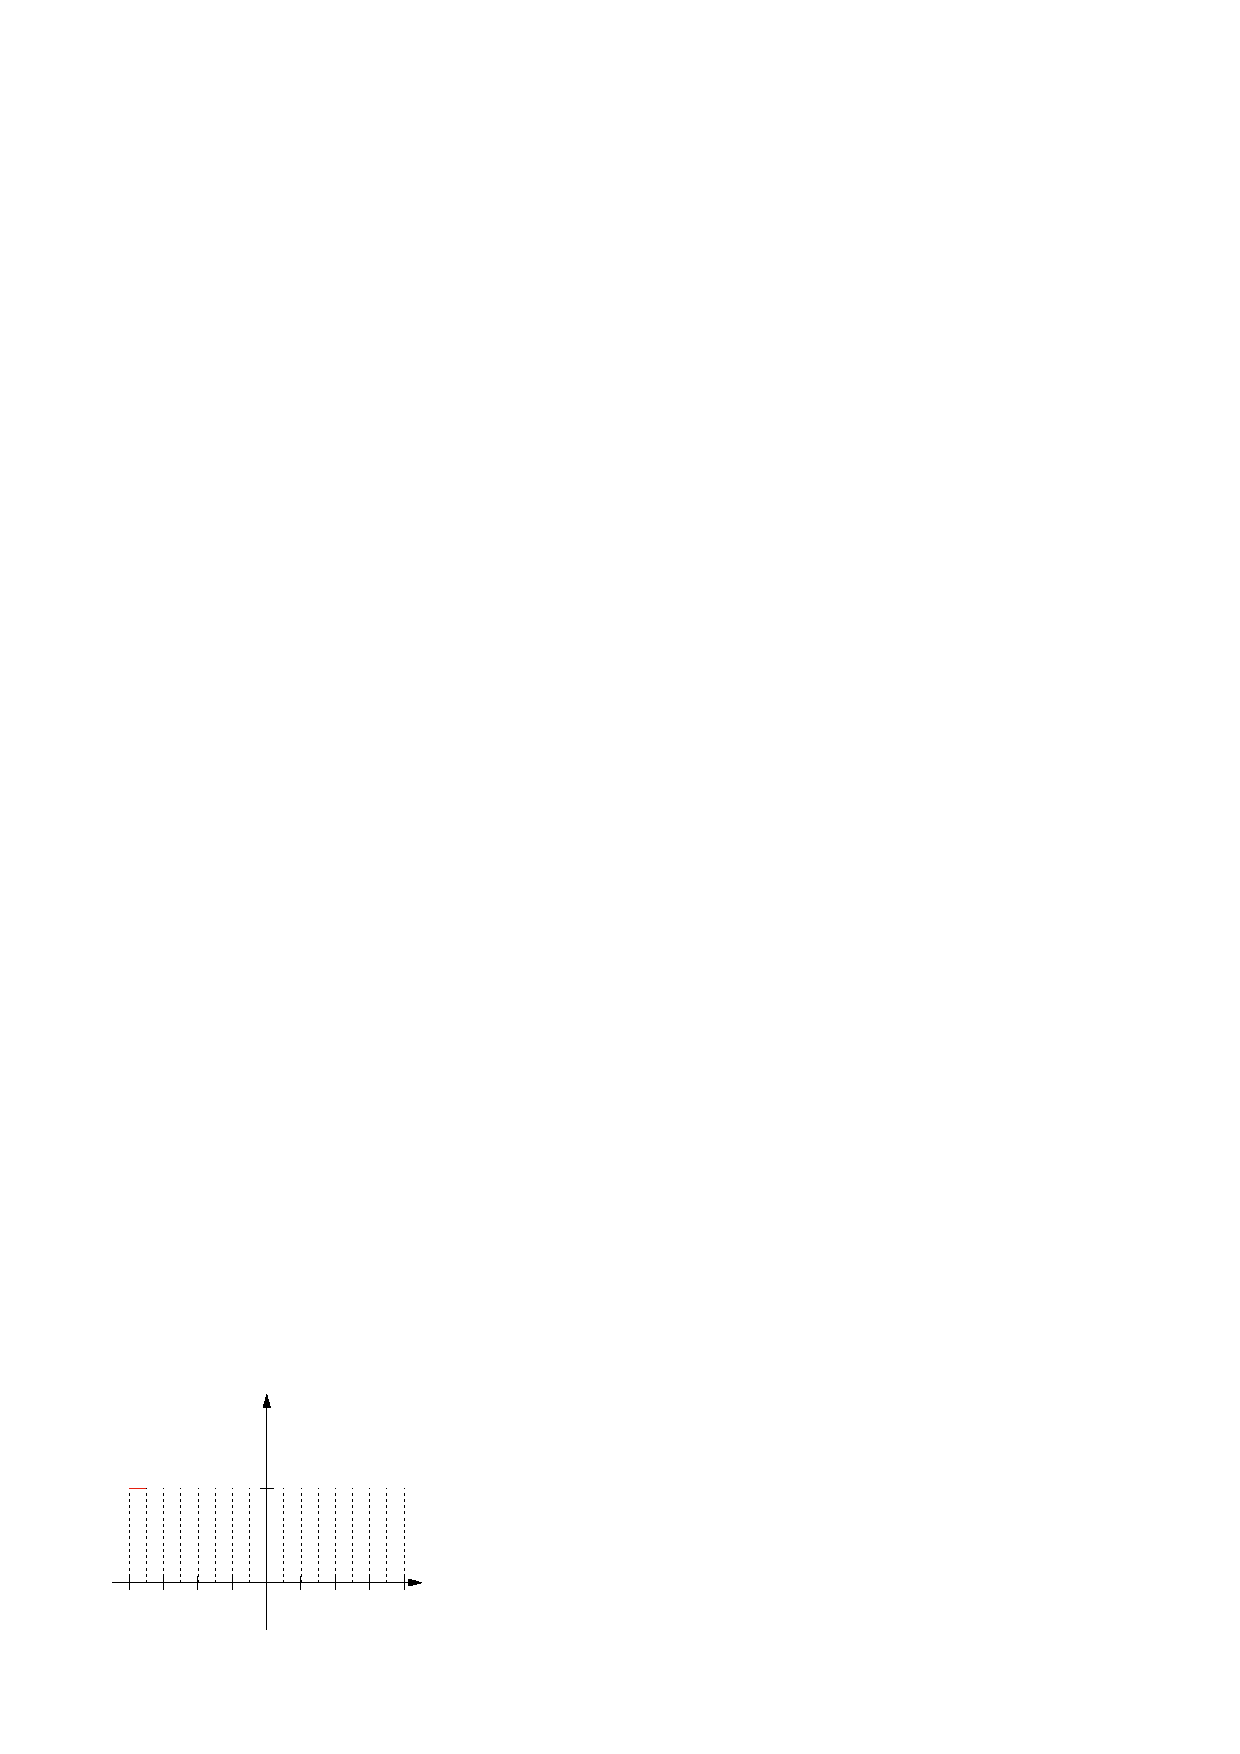
\includegraphics[width={158.40bp},height={108.00bp}]{figura_04_04}}%
    \gplfronttext
  \end{picture}%
\endgroup

    \end{minipage}
\end{figure}

\section{Propiedades de la transformada de \emph{Fourier}}
\subsection{Linealidad}
\begin{equation}
    \mathcal{F}\{a_1f_1(t)+a_2f_2(t)\}=a_1F_1(\omega)+a_2F_2(\omega)
\end{equation}

Donde:
\begin{equation*}
    F_1(\omega)=\mathcal{F}\{f_1(t)\}
\end{equation*}
\begin{equation*}
    F_2(\omega)=\mathcal{F}\{f_2(t)\}
\end{equation*}

\subsection{Cambio de escala}
Si: $\mathcal{F}\{f(t)\}=F(\omega)$:
\begin{equation}
    \mathcal{F}\{f(at)\}=\frac{1}{|a|}F\left(\frac{\omega}{a}\right)
\end{equation}

\underline{Prueba}:

\begin{equation*}
    \mathcal{F}\{f(at)\}=\int_{-\infty}^\infty f(at)\,e^{-j\omega t}\,dt
\end{equation*}

Realizando un cambio de variable:
\begin{equation*}
    \tau=at
\end{equation*}
\begin{equation*}
    d\tau=a\,dt
\end{equation*}

Para $a>0$:
\begin{equation*}
\begin{split}
    \mathcal{F}\{f(at)\}
        &=\int_{-\infty}^\infty f(\tau)\,e^{-j\omega
            \frac{\tau}{a}}\,\frac{d\tau}{a}\\
        &=\frac{1}{a}\int_{-\infty}^\infty f(\tau)\,e^{-j\omega
            \frac{\tau}{a}}d\tau\\
        &=\frac{1}{a}F\left(\frac{\omega}{a}\right)\\
\end{split}
\end{equation*}

Para $a<0$:
\begin{equation*}
\begin{split}
    \mathcal{F}\{f(at)\}
        &=\int_\infty^{-\infty} f(\tau)\,e^{-j\omega
            \frac{\tau}{a}}\,\frac{d\tau}{a}\\
        &=-\frac{1}{a}\int_{-\infty}^\infty f(\tau)\,e^{-j\omega
            \frac{\tau}{a}}d\tau\\
        &=-\frac{1}{a}F\left(\frac{\omega}{a}\right)\\
\end{split}
\end{equation*}

\subsection{Desplazamiento en $\omega$}
Si: $\mathcal{F}\{f(t)\}=F(\omega)$:
\begin{equation}
    \mathcal{F}\{f(t)\,e^{jat}\}=F(\omega-a)
\end{equation}

\underline{Prueba}:

\begin{equation*}
\begin{split}
    \mathcal{F}\{f(t)\,e^{jat}\}
        &=\int_{-\infty}^\infty f(t)\,e^{jat}\,e^{-j\omega t}\,dt\\
        &=\int_{-\infty}^\infty f(t)\,e^{-j(\omega-a)t}\,dt\\
        &=F(\omega-a)\\
\end{split}
\end{equation*}

\subsection{Desplazamiento en $t$}
Si: $\mathcal{F}\{f(t)\}=F(\omega)$:
\begin{equation}
    \mathcal{F}\{f(t-a)\}=F(\omega)\,e^{-ja\omega}
\end{equation}

\underline{Prueba}:

\begin{equation*}
    \mathcal{F}\{f(t-a)\}=\int_{-\infty}^\infty f(t-a)\,e^{-j\omega t}\,dt
\end{equation*}

Realizando un cambio de variable:
\begin{equation*}
    \tau=t-a
\end{equation*}
\begin{equation*}
    d\tau=dt
\end{equation*}

\begin{equation*}
\begin{split}
    \mathcal{F}\{f(t-a)\}
        &=\int_{-\infty}^\infty f(\tau)\,e^{-j\omega(\tau+a)}\,dt\\
        &=e^{-ja\omega}\int_{-\infty}^\infty f(\tau)\,e^{-j\omega\tau}\,d\tau\\
        &=e^{-ja\omega}F(\omega)\\
\end{split}
\end{equation*}

\subsection{Simetría}
Si: $\mathcal{F}\{f(t)\}=F(\omega)$:
\begin{equation}
    \mathcal{F}\{F(t)\}=2\pi f(-\omega)
\end{equation}

\underline{Prueba}:

\begin{equation*}
    f(t)=\frac{1}{2\pi}\int_{-\infty}^\infty F(\omega)\,e^{j\omega t}\,d\omega
\end{equation*}

Reemplazando:
\begin{equation*}
    t\to-\omega
\end{equation*}
\begin{equation*}
    \omega\to t
\end{equation*}

\begin{equation*}
\begin{split}
    f(-\omega)=
        &=\frac{1}{2\pi}\int_{-\infty}^\infty F(t)\,e^{jt(-\omega)}\,dt\\
        &=\frac{1}{2\pi}\mathcal{F}\{F(t)\}\\
\end{split}
\end{equation*}
\begin{equation*}
    2\pi f(-\omega)=\mathcal{F}\{F(t)\}
\end{equation*}

\textbf{Ejemplo 2:} Hallar $\mathcal{F}\{\dfrac{\sen(at)}{t}\}$
Sabiendo que:
\begin{equation*}
    \mathcal{F}\{u(t+a)-u(t-a)\}=\dfrac{2\sen(a\omega)}{\omega}
\end{equation*}
\begin{equation*}
    \mathcal{F}\{\dfrac{2\sen(at)}{t}\}=2\pi(u(t+a)-u(t-a))
\end{equation*}
\begin{equation}
    \mathcal{F}\{\dfrac{\sen(at)}{t}\}=\pi(u(t+a)-u(t-a))
\end{equation}

\subsection{Multiplicación por $t$}
Si: $\mathcal{F}\{f(t)\}=F(\omega)$:
\begin{equation*}
    \mathcal{F}\{t\,f(t)\}=j\frac{dF(\omega)}{d\omega}
\end{equation*}

En general:
\begin{equation}
    \mathcal{F}\{t^n\,f(t)\}=j^n\frac{d^{(n)}F(\omega)}{d\omega^n};
    \quad n\in\mathbb{N}
\end{equation}

\underline{Prueba}:

\begin{equation*}
    F(\omega)=\int_{-\infty}^\infty f(t)\,e^{-j\omega t}\,dt
\end{equation*}

\begin{equation*}
\begin{split}
    \frac{dF(\omega)}{d\omega}
        &=\int_{-\infty}^\infty f(t)\,e^{-j\omega t}(-jt)\,dt\\
        &=-j\int_{-\infty}^\infty t\,f(t)\,e^{-j\omega t}\,dt\\
        &=-j\,\mathcal{F}\{t\,f(t)\}\\
\end{split}
\end{equation*}
\begin{equation*}
    j\frac{dF(\omega)}{d\omega}=\mathcal{F}\{t\,f(t)\}
\end{equation*}
\begin{equation*}
\begin{split}
    \mathcal{F}\{t^2\,f(t)\}
        &=\mathcal{F}\{t\,t\,f(t)\}\\
        &=j\frac{d}{d\omega}\left(\mathcal{F}\{t\,f(t)\}\right)\\
        &=j\frac{d}{d\omega}\left(j\frac{dF(\omega)}{d\omega}\right)\\
        &=j^2\frac{d^2F(\omega)}{d\omega^2}\\
\end{split}
\end{equation*}
\begin{equation*}
    \mathcal{F}\{t^n\,f(t)\}=j^n\frac{d^n F(\omega)}{d\omega^n}\\
\end{equation*}

\textbf{Ejemplo 3:} Hallar $\mathcal{F}\{t^n e^{-at} u(t)\};
\quad n\in\mathbb{N}$

Para $n=1$:
\begin{equation*}
\begin{split}
    \mathcal{F}\{t\,e^{-at} u(t)\}
        &=j\frac{d}{d\omega}\left(\frac{1}{a+j\omega}\right)\\
        &=(j)(-1){(a+j\omega)}^{-2}(j)\\
        &=\frac{1}{{(a+j\omega)}^2}\\
\end{split}
\end{equation*}

Para $n=2$:
\begin{equation*}
\begin{split}
    \mathcal{F}\{t^2\,e^{-at} u(t)\}
        &=j\frac{d}{d\omega}\left(\frac{1}{{(a+j\omega)}^2}\right)\\
        &=(j)(-2){(a+j\omega)}^{-3}(j)\\
        &=\frac{2}{{(a+j\omega)}^3}\\
\end{split}
\end{equation*}

Para $n=3$:
\begin{equation*}
\begin{split}
    \mathcal{F}\{t^3\,e^{-at} u(t)\}
        &=j\frac{d}{d\omega}\left(\frac{2}{{(a+j\omega)}^3}\right)\\
        &=(j)(2)(-3){(a+j\omega)}^{-4}(j)\\
        &=\frac{6}{{(a+j\omega)}^4}\\
\end{split}
\end{equation*}

Por tanto:
\begin{equation}
    \mathcal{F}\{t^n\,e^{-at} u(t)\}=\frac{n!}{{(a+j\omega)}^{n+1}}
\end{equation}

\subsection{Transformada de \emph{Fourier} de una derivada}
Si: $\mathcal{F}\{f(t)\}=F(\omega)$:
\begin{equation*}
    \mathcal{F}\{f'(t)\}=j\omega F(\omega)
\end{equation*}

En general:
\begin{equation}
    \mathcal{F}\{f^{(n)}(t)\}={(j\omega)}^n F(\omega)
    \quad n\in\mathbb{N}
\end{equation}

\underline{Prueba}:

\begin{equation*}
    \mathcal{F}\{f'(t)\}=\int_{\infty}^\infty f'(t)\,e^{-j\omega t}\,dt
\end{equation*}

Realizando la integración por partes:
\begin{equation*}
    u=e^{-j\omega t}
\end{equation*}
\begin{equation*}
    du=-j\omega\,e^{-j\omega t}\,dt
\end{equation*}
\begin{equation*}
    dv=f'(t)\,dt
\end{equation*}
\begin{equation*}
    v=f(t)
\end{equation*}
\begin{equation*}
    \mathcal{F}\{f'(t)\}
        =\left(f(t)\,e^{-j\omega t}\Biggr|_{-\infty}^\infty\right)
        -\int_{-\infty}^\infty f(t)\,(-j\omega\,e^{-j\omega t})\,dt
\end{equation*}

Asumiendo $f(\pm\infty)=0$:
\begin{equation*}
\begin{split}
    \mathcal{F}\{f'(t)\}
        &=j\omega\int_{-\infty}^\infty f(t)\,e^{-j\omega t}\,dt\\
        &=j\omega\,F(\omega)\\
\end{split}
\end{equation*}

Para la segunda derivada:
\begin{equation*}
\begin{split}
    \mathcal{F}\{f^{\prime\prime}(t)\}
        &=\mathcal{F}\{(f'(t))'\}\\
        &=j\omega\,\mathcal{F}\{f'(t)\}\\
        &=j\omega(j\omega\,F(\omega))\\
        &={(j\omega)}^2\,F(\omega)\\
\end{split}
\end{equation*}

Por tanto:
\begin{equation*}
    \mathcal{F}\{f^{(n)}(t)\}={(j\omega)}^n F(\omega)
\end{equation*}

\section{Transformadas de \emph{Fourier} especiales}
\subsection{$e^{-at}\,u(t);\quad a>0$}
\begin{equation*}
    \mathcal{F}\{e^{-at}\,u(t)\}; a>0
\end{equation*}
\begin{equation*}
\begin{split}
    \mathcal{F}\{e^{-at}\,u(t)\}
        &=\int_0^\infty e^{-at}\,e^{-j\omega t}\,dt\\
        &=\int_0^\infty e^{-(a+j\omega)t}\,dt\\
        &=\frac{e^{-(a+j\omega)t}}{-(a+j\omega)}\Biggr|_0^\infty\\
        &=\frac{0-1}{-(a+j\omega)}\\
        &=\frac{1}{a+j\omega}\\
\end{split}
\end{equation*}
\begin{equation}
    \mathcal{F}\{e^{-at}\,u(t)\}=\frac{1}{a+j\omega}\\
\end{equation}

\subsection{$e^{at}\,u(-t);\quad a>0$}
\begin{equation*}
    \mathcal{F}\{e^{at}\,u(-t)\}; a>0
\end{equation*}
\begin{equation*}
\begin{split}
    \mathcal{F}\{e^{at}\,u(t)\}
        &=\int_{-\infty}^0 e^{at}\,e^{-j\omega t}\,dt\\
        &=\int_{-\infty}^0 e^{(a-j\omega)t}\,dt\\
        &=\frac{e^{(a-j\omega)t}}{a-j\omega}\Biggr|_{-\infty}^0\\
        &=\frac{1}{a-j\omega}\\
\end{split}
\end{equation*}
\begin{equation}
    \mathcal{F}\{e^{at}\,u(-t)\}=\frac{1}{a-j\omega}\\
\end{equation}

\subsection{$e^{-a|t|}$}
\begin{equation*}
    \mathcal{F}\{e^{-a|t|}\}
\end{equation*}
\begin{equation*}
\begin{split}
    \mathcal{F}\{e^{-a|t|}\}
        &=\mathcal{F}\{e^{at}u(-t)+e^{-at}u(t)\}\\
        &=\frac{1}{a-j\omega}+\frac{1}{a+j\omega}\\
        &=\frac{a+j\omega+a-j\omega}{(a-j\omega)(a+j\omega)}\\
        &=\frac{2a}{a^2+\omega^2}
\end{split}
\end{equation*}
\begin{equation}
    \mathcal{F}\{e^{-a|t|}\}=\frac{2a}{a^2+\omega^2}
\end{equation}

\subsection{$\delta(t-t_0)$}
\begin{equation*}
    \mathcal{F}\{\delta(t-t_0)\}
\end{equation*}
\begin{equation*}
\begin{split}
    \mathcal{F}\{\delta(t-t_0)\}
        &=\int_{-\infty}^0\delta(t-t_0)\,e^{-j\omega t}\,dt\\
        &=e^{-j\omega t_0}\\
\end{split}
\end{equation*}
\begin{equation}
    \mathcal{F}\{\delta(t-t_0)\}=e^{-j\omega t_0}
\end{equation}

En particular:
\begin{equation*}
    \mathcal{F}\{\delta(t)\}=1
\end{equation*}

\subsection{$e^{jat}$}
Sabiendo:
\begin{equation*}
    \mathcal{F}\{\delta(t-a)\}=e^{-ja\omega}
\end{equation*}

Aplicando la propiedad de simetría:
\begin{equation*}
    \mathcal{F}\{e^{-jat}\}=2\pi\delta(-\omega-a)\
\end{equation*}
\begin{equation*}
\begin{split}
    \mathcal{F}\{e^{jat}\}
        &=2\pi\delta(-\omega+a)\\
        &=2\pi\delta(-(\omega-a))\\
        &=2\pi\delta(\omega-a)\\
\end{split}
\end{equation*}
\begin{equation}
    \mathcal{F}\{e^{jat}\}=2\pi\delta(\omega-a)
\end{equation}

En particular:
\begin{equation*}
    \mathcal{F}\{1\}=2\pi\delta(\omega)
\end{equation*}
\begin{equation*}
    \mathcal{F}\{k\}=2\pi k\delta(\omega)
\end{equation*}

\subsection{$\sen(at)$}
\begin{equation*}
\begin{split}
    \mathcal{F}\{\sen(at)\}
        &=\mathcal{F}\{\frac{e^{jat}-e^{-jat}}{2j}\}\\
        &=\frac{1}{2j}\left(2\pi\delta(\omega-a)-2\pi\delta(\omega+a)\right)\\
        &=-j\pi(\delta(\omega-a)-\delta(\omega+a))
\end{split}
\end{equation*}
\begin{equation}
    \mathcal{F}\{\sen(at)\}=j\pi(\delta(\omega+a)+\delta(\omega-a))
\end{equation}

\subsection{$\cos(at)$}
\begin{equation*}
\begin{split}
    \mathcal{F}\{\cos(at)\}
        &=\mathcal{F}\{\frac{e^{jat}+e^{-jat}}{2}\}\\
        &=\frac{1}{2}\left(2\pi\delta(\omega-a)+2\pi\delta(\omega+a)\right)\\
        &=\pi(\delta(\omega+a)+\delta(\omega-a))
\end{split}
\end{equation*}
\begin{equation}
    \mathcal{F}\{\cos(at)\}=\pi(\delta(\omega+a)+\delta(\omega-a))
\end{equation}

\subsection{$u(t)$}
\begin{equation*}
    u(t)+u(-t)=1
\end{equation*}
\begin{equation*}
    \mathcal{F}\{u(t)+u(-t)\}=\mathcal{F}\{1\}
\end{equation*}

Considerando:
\begin{equation*}
    \mathcal{F}\{u(t)\}=F(\omega)
\end{equation*}
\begin{equation*}
    \mathcal{F}\{u(-t)\}=F(-\omega)
\end{equation*}

Por tanto:
\begin{equation*}
    F(\omega)+F(-\omega)=2\pi\delta(\omega)
\end{equation*}

Se asume que la transformada de \emph{Fourier} de la función escalón tendrá un
termino impulsivo:
\begin{equation*}
    F(\omega)=\beta(\omega)+k\delta(\omega)
\end{equation*}
\begin{equation*}
    F(-\omega)=\beta(-\omega)+k\delta(\omega)
\end{equation*}
\begin{equation*}
    F(\omega)+F(-\omega)=\beta(\omega)+\beta(-\omega)+2k\delta(\omega)
\end{equation*}

Reemplazando:
\begin{equation*}
    \beta(\omega)+\beta(-\omega)+2k\delta(\omega)=2\pi\delta(\omega)
\end{equation*}

Por tanto:
\begin{equation*}
    k=\pi
\end{equation*}

Resultando:
\begin{equation*}
    F(\omega)=\beta(\omega)+\pi\delta(\omega)
\end{equation*}

Por otro lado, se sabe que:
\begin{equation*}
    u'(t)=\delta(t)
\end{equation*}
\begin{equation*}
    \mathcal{F}\{u'(t)\}=\mathcal{F}\{\delta(t)\}
\end{equation*}
\begin{equation*}
    j\omega\mathcal{F}\{u(t)\}=1
\end{equation*}
\begin{equation*}
    j\omega(\beta(\omega)+\pi\delta(\omega))=1
\end{equation*}
\begin{equation*}
    j\omega\beta(\omega)+j\pi\omega\delta(\omega)=1
\end{equation*}
\begin{equation*}
    j\omega\beta(\omega)=1
\end{equation*}
\begin{equation*}
    \beta(\omega)=\frac{1}{j\omega}
\end{equation*}
\begin{equation}
    \mathcal{F}\{u(t)\}=\frac{1}{j\omega}+\pi\delta(\omega)
\end{equation}

\section{La función signo}
\begin{equation}
    sgn(t)=\begin{cases}
        -1 & t<0\\
        1 & t>0\\
    \end{cases}
\end{equation}
\begin{figure}[H]
    \centering
    % GNUPLOT: LaTeX picture with Postscript
\begingroup
  \makeatletter
  \providecommand\color[2][]{%
    \GenericError{(gnuplot) \space\space\space\@spaces}{%
      Package color not loaded in conjunction with
      terminal option `colourtext'%
    }{See the gnuplot documentation for explanation.%
    }{Either use 'blacktext' in gnuplot or load the package
      color.sty in LaTeX.}%
    \renewcommand\color[2][]{}%
  }%
  \providecommand\includegraphics[2][]{%
    \GenericError{(gnuplot) \space\space\space\@spaces}{%
      Package graphicx or graphics not loaded%
    }{See the gnuplot documentation for explanation.%
    }{The gnuplot epslatex terminal needs graphicx.sty or graphics.sty.}%
    \renewcommand\includegraphics[2][]{}%
  }%
  \providecommand\rotatebox[2]{#2}%
  \@ifundefined{ifGPcolor}{%
    \newif\ifGPcolor
    \GPcolorfalse
  }{}%
  \@ifundefined{ifGPblacktext}{%
    \newif\ifGPblacktext
    \GPblacktexttrue
  }{}%
  % define a \g@addto@macro without @ in the name:
  \let\gplgaddtomacro\g@addto@macro
  % define empty templates for all commands taking text:
  \gdef\gplbacktext{}%
  \gdef\gplfronttext{}%
  \makeatother
  \ifGPblacktext
    % no textcolor at all
    \def\colorrgb#1{}%
    \def\colorgray#1{}%
  \else
    % gray or color?
    \ifGPcolor
      \def\colorrgb#1{\color[rgb]{#1}}%
      \def\colorgray#1{\color[gray]{#1}}%
      \expandafter\def\csname LTw\endcsname{\color{white}}%
      \expandafter\def\csname LTb\endcsname{\color{black}}%
      \expandafter\def\csname LTa\endcsname{\color{black}}%
      \expandafter\def\csname LT0\endcsname{\color[rgb]{1,0,0}}%
      \expandafter\def\csname LT1\endcsname{\color[rgb]{0,1,0}}%
      \expandafter\def\csname LT2\endcsname{\color[rgb]{0,0,1}}%
      \expandafter\def\csname LT3\endcsname{\color[rgb]{1,0,1}}%
      \expandafter\def\csname LT4\endcsname{\color[rgb]{0,1,1}}%
      \expandafter\def\csname LT5\endcsname{\color[rgb]{1,1,0}}%
      \expandafter\def\csname LT6\endcsname{\color[rgb]{0,0,0}}%
      \expandafter\def\csname LT7\endcsname{\color[rgb]{1,0.3,0}}%
      \expandafter\def\csname LT8\endcsname{\color[rgb]{0.5,0.5,0.5}}%
    \else
      % gray
      \def\colorrgb#1{\color{black}}%
      \def\colorgray#1{\color[gray]{#1}}%
      \expandafter\def\csname LTw\endcsname{\color{white}}%
      \expandafter\def\csname LTb\endcsname{\color{black}}%
      \expandafter\def\csname LTa\endcsname{\color{black}}%
      \expandafter\def\csname LT0\endcsname{\color{black}}%
      \expandafter\def\csname LT1\endcsname{\color{black}}%
      \expandafter\def\csname LT2\endcsname{\color{black}}%
      \expandafter\def\csname LT3\endcsname{\color{black}}%
      \expandafter\def\csname LT4\endcsname{\color{black}}%
      \expandafter\def\csname LT5\endcsname{\color{black}}%
      \expandafter\def\csname LT6\endcsname{\color{black}}%
      \expandafter\def\csname LT7\endcsname{\color{black}}%
      \expandafter\def\csname LT8\endcsname{\color{black}}%
    \fi
  \fi
    \setlength{\unitlength}{0.0500bp}%
    \ifx\gptboxheight\undefined%
      \newlength{\gptboxheight}%
      \newlength{\gptboxwidth}%
      \newsavebox{\gptboxtext}%
    \fi%
    \setlength{\fboxrule}{0.5pt}%
    \setlength{\fboxsep}{1pt}%
    \definecolor{tbcol}{rgb}{1,1,1}%
\begin{picture}(4320.00,2014.00)%
    \gplgaddtomacro\gplbacktext{%
      \csname LTb\endcsname%%
      \put(2040,469){\makebox(0,0)[r]{\strut{}}}%
      \put(2040,1023){\makebox(0,0)[r]{\strut{}}}%
      \put(2040,1576){\makebox(0,0)[r]{\strut{}}}%
      \put(240,800){\makebox(0,0){\strut{}}}%
      \put(619,800){\makebox(0,0){\strut{}}}%
      \put(998,800){\makebox(0,0){\strut{}}}%
      \put(1377,800){\makebox(0,0){\strut{}}}%
      \put(1756,800){\makebox(0,0){\strut{}}}%
      \put(2136,800){\makebox(0,0){\strut{}}}%
      \put(2515,800){\makebox(0,0){\strut{}}}%
      \put(2894,800){\makebox(0,0){\strut{}}}%
      \put(3273,800){\makebox(0,0){\strut{}}}%
      \put(3652,800){\makebox(0,0){\strut{}}}%
      \put(4031,800){\makebox(0,0){\strut{}}}%
      \csname LTb\endcsname%%
      \put(4600,1023){\makebox(0,0)[l]{\strut{}$t$}}%
      \put(2325,1798){\makebox(0,0)[l]{\strut{}$f(t)$}}%
      \put(1946,1576){\makebox(0,0)[l]{\strut{}$1$}}%
      \put(2287,469){\makebox(0,0)[l]{\strut{}$-1$}}%
    }%
    \gplgaddtomacro\gplfronttext{%
    }%
    \gplgaddtomacro\gplbacktext{%
      \csname LTb\endcsname%%
      \put(2040,469){\makebox(0,0)[r]{\strut{}}}%
      \put(2040,1023){\makebox(0,0)[r]{\strut{}}}%
      \put(2040,1576){\makebox(0,0)[r]{\strut{}}}%
      \put(240,800){\makebox(0,0){\strut{}}}%
      \put(619,800){\makebox(0,0){\strut{}}}%
      \put(998,800){\makebox(0,0){\strut{}}}%
      \put(1377,800){\makebox(0,0){\strut{}}}%
      \put(1756,800){\makebox(0,0){\strut{}}}%
      \put(2136,800){\makebox(0,0){\strut{}}}%
      \put(2515,800){\makebox(0,0){\strut{}}}%
      \put(2894,800){\makebox(0,0){\strut{}}}%
      \put(3273,800){\makebox(0,0){\strut{}}}%
      \put(3652,800){\makebox(0,0){\strut{}}}%
      \put(4031,800){\makebox(0,0){\strut{}}}%
      \csname LTb\endcsname%%
      \put(4600,1023){\makebox(0,0)[l]{\strut{}$t$}}%
      \put(2325,1798){\makebox(0,0)[l]{\strut{}$f(t)$}}%
      \put(1946,1576){\makebox(0,0)[l]{\strut{}$1$}}%
      \put(2287,469){\makebox(0,0)[l]{\strut{}$-1$}}%
    }%
    \gplgaddtomacro\gplfronttext{%
    }%
    \gplbacktext
    \put(0,0){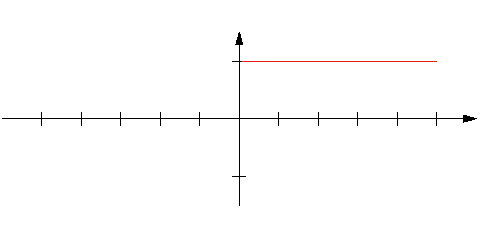
\includegraphics[width={216.00bp},height={100.70bp}]{figura_04_05}}%
    \gplfronttext
  \end{picture}%
\endgroup

\end{figure}

Esta función puede representarse también como:
\begin{equation*}
    sgn(t)=\frac{|t|}{t}
\end{equation*}
\begin{equation*}
    sgn(t)=-1+2u(t)
\end{equation*}

A partir de la definición de la función de valor absoluto:
\begin{equation*}
    |t|=\begin{cases}
        -t & t<0\\
        t & t>0\\
    \end{cases}
\end{equation*}

Es posible calcular la derivada del valor absoluto:
\begin{equation*}
    |t|'=\begin{cases}
        -1 & t<0\\
        1 & t>0\\
    \end{cases}
\end{equation*}

Por tanto:
\begin{equation}
    |t|'=sgn(t)
\end{equation}

Cuya derivada es:
\begin{equation}
    sgn'(t)=2\delta(t)
\end{equation}

Calculando su transformada de \emph{Fourier}:
\begin{equation*}
\begin{split}
    \mathcal{F}\{sgn(t)\}
        &=\mathcal{F}\{-1+2u(t)\}\\
        &=-2\pi\delta(\omega)
            +2\left(\frac{1}{j\omega}+\pi\delta(\omega)\right)\\
        &=-2\pi\delta(\omega)
            +2\left(\frac{1}{j\omega}\right)+2\pi\delta(\omega)\\
        &=\frac{2}{j\omega}
\end{split}
\end{equation*}
\begin{equation}
    \mathcal{F}\{sgn(t)\}=\frac{2}{j\omega}
\end{equation}

\subsection{Transformada de \emph{Fourier} de $|t|$}
\begin{equation*}
    \mathcal{F}\{|t|'\}=\mathcal{F}\{sgn(t)\}
\end{equation*}
\begin{equation*}
    j\omega\mathcal{F}\{|t|\}=\frac{2}{j\omega}
\end{equation*}
\begin{equation}
    \mathcal{F}\{|t|\}=-\frac{2}{j\omega^2}
\end{equation}

\subsection{Transformada de \emph{Fourier} de $1/t$}
\begin{equation*}
    \mathcal{F}\{sgn(t)\}=\frac{2}{j\omega}
\end{equation*}

Por simetría:
\begin{equation*}
    \mathcal{F}\{\frac{2}{jt}\}=2\pi\,sgn(-\omega)
\end{equation*}
\begin{equation}
    \mathcal{F}\{\frac{1}{t}\}=-j\pi\,sgn(-\omega)
\end{equation}

Calculando la segunda derivada:
\begin{equation*}
    \left(\frac{1}{t}\right)'=-\frac{1}{t^2}
\end{equation*}
\begin{equation*}
    \mathcal{F}\{-\frac{1}{t^2}\}=j\omega(-j\pi\,sgn(\omega))
\end{equation*}
\begin{equation*}
    \mathcal{F}\{-\frac{1}{t^2}\}=j^2\pi\omega\,sgn(\omega)
\end{equation*}

Calculando la derivada n-ésima:
\begin{equation*}
    {\left(\frac{1}{t}\right)}^{\prime\prime}=\frac{2}{t^3}
\end{equation*}
\begin{equation*}
    {\left(\frac{1}{t}\right)}^{\prime\prime\prime}=-\frac{6}{t^4}
\end{equation*}
\begin{equation*}
    {\left(\frac{1}{t}\right)}^{(n)}={(-1)}^k \frac{k!}{t^{k+1}}
\end{equation*}
\begin{equation*}
    \mathcal{F}\{f^{(k)}(t)\}={(-1)}^k\,k!\,\mathcal{F}\{\frac{1}{t^{k+1}}\}
\end{equation*}
\begin{equation*}
    {(j\omega)}^k(-j\pi\,sgn(\omega))={(-1)}^k\,k!\,\mathcal{F}\{\frac{1}{t^{k+1}}\}
\end{equation*}
\begin{equation*}
    -j^{k+1}\pi\omega^k\,sgn(\omega)={(-1)}^k\,k!\,\mathcal{F}\{\frac{1}{t^{k+1}}\}
\end{equation*}
\begin{equation*}
    -j^n\pi\omega^{n-1}\,sgn(\omega)={(-1)}^{n-1}\,(n-1)!\,\mathcal{F}\{\frac{1}{t^n}\}
\end{equation*}
\begin{equation*}
    -j^n\pi\omega^{n-1}\,sgn(\omega)={(-1)}^n{(-1)}^{-1}(n-1)!\mathcal{F}\{\frac{1}{t^n}\}
\end{equation*}
\begin{equation}
    \mathcal{F}\{\frac{1}{t^n}\}=\frac{j^n\pi{\omega}^{n-1}\,sgn(\omega)}{{(-1)}^n(n-1)!}
\end{equation}

\section{Tabla de transformadas de \emph{Fourier} conocidas}

\begin{equation*}
\def\arraystretch{1.3}
\begin{array}{@{}lll@{}}
\toprule
 & f(t) & F(\omega)=\mathcal{F}\{f(t)\} \\
\cmidrule(l){2-3}
 1 & u(t+a)-u(t-a)
   & \dfrac{2\sen(a\omega)}{\omega}\\
 2 & \dfrac{\sen(at)}{t}
   & \pi[u(\omega+a)-u(\omega-a)]\\
 3 & e^{-at}\,u(t)\quad a>0
   & \dfrac{1}{a+j\omega}\\
 4 & e^{at}\,u(-t)\quad a>0
   & \dfrac{1}{a-j\omega}\\
 5 & e^{-a|t|}\quad a>0
   & \dfrac{2a}{a^2+\omega^2}\\
 6 & \dfrac{1}{t^2+a^2}
   & \dfrac{\pi}{a}e^{-a|\omega|}\\
 7 & \delta(t-a)
   & e^{-ja\omega}\\
 8 & e^{jat}
   & 2\pi\delta(\omega-a)\\
 9 & k
   & 2\pi k\delta(\omega)\\
10 & \sen(at)
   & j\omega[\delta(\omega+a)-\delta(\omega-a)]\\
11 & \cos(at)
   & \pi[\delta(\omega+a)+\delta(\omega-a)]\\
12 & t^n\,e^{-at}\,u(t)
   & \dfrac{n!}{{(a+j\omega)}^{n+1}}\quad n\in\mathbb{N}\\
13 & u(t)
   & \dfrac{1}{j\omega}+\pi\delta(\omega)\\
14 & sgn(t)
   & \dfrac{2}{j\omega}\\
15 & |t|
   & -\dfrac{2}{\omega^2}\\
16 & \dfrac{1}{t}
   & -j\pi\,sgn(\omega)\\
17 & \dfrac{1}{t^n}
   & \dfrac{j^n\pi{\omega}^{n-1}\,sgn(\omega)}{{(-1)}^n(n-1)!}\\
\bottomrule
\end{array}
\end{equation*}


%\chapter{Transformada inversa de \emph{Fourier}}

\begin{equation}
    \mathcal{F}\{f(t)\}=F(\omega)
    \rightarrow
    \mathcal{F}^{-1}\{F(\omega)\}=f(t)
\end{equation}

Con la transformada inversa de \emph{Fourier} se regresa del dominio de
``$\omega$'' al dominio de ``$t$''.

\section{Tabla de transformadas de \emph{Fourier} inversas}

\begin{equation*}
\def\arraystretch{1.4}
\begin{array}{@{}cll@{}}
\toprule
 & F(\omega) & f(t)=\mathcal{F}^{-1}\{F(\omega)\}\\
\cmidrule(l){1-3}
 1 & \dfrac{1}{a+j\omega}
   & e^{-at}\,u(t)\quad\,a>0\\
\cmidrule(l){1-3}
 2 & \dfrac{1}{a-j\omega}
   & e^{at}\,u(-t)\quad\,a>0\\
\cmidrule(l){1-3}
 3 & \dfrac{2a}{a^2+\omega^2}
   & e^{-a|t|}\quad\,a>0\\
\cmidrule(l){1-3}
 4 & \frac{1}{\omega}\sen(a\omega)
   & \frac{1}{2}[u(t+a)-u(t-a)]\\
\cmidrule(l){1-3}
 5 & k
   & k\delta(t)\\
\cmidrule(l){1-3}
 6 & \dfrac{1}{\omega}
   & \frac{1}{2}j\,\sgn(t)\\
\bottomrule
\end{array}
\end{equation*}

\section{Propiedades de la transformada inversa de \emph{Fourier}}

\subsection{Linealidad}
\begin{equation}
    \mathcal{F}^{-1}\{a_1\,F_1(\omega)+a_2\,F_2(\omega)\}
    =a_1\,f_1(t)+a_2\,f_2(t)
\end{equation}

\subsection{Desplazamiento en $t$}
Si $\mathcal{F}^{-1}\{F(\omega)\}=f(t)$:
\begin{equation}
    \mathcal{F}^{-1}\{F(\omega)\,e^{-ja\omega}\}=f(t-a)
\end{equation}

\subsection{Desplazamiento en $\omega$}
Si $\mathcal{F}^{-1}\{F(\omega)\}=f(t)$:
\begin{equation}
    \mathcal{F}^{-1}\{F(\omega-a)\}=f(t)\,e^{jat}
\end{equation}

\section{Convolución}
Dadas dos funciones $f_1(t)$ y $f_2(t)$ definimos la convolución mediante la
siguiente integral:

\begin{equation}
    f(t)=f_1(t)*f_2(t)=\int_{-\infty}^{\infty}f_1(\tau)\,f_2(t-\tau)\,d\tau
\end{equation}

\begin{itemize}
    \item En $f_1(t)$ se reemplaza ``$t$'' por ``$\tau$'', permanece fija y no
    cambia.
    \item En $f_2(t)$ se reemplaza ``$t$'' por ``$t-\tau$''.La gráfica se
    refleja respecto al eje vertical, y luego se desplaza un ``$t$'' variable.
\end{itemize}

\begin{figure}[H]
    \centering
    \begin{minipage}{.4\textwidth}
        \centering
        % GNUPLOT: LaTeX picture with Postscript
\begingroup
  \makeatletter
  \providecommand\color[2][]{%
    \GenericError{(gnuplot) \space\space\space\@spaces}{%
      Package color not loaded in conjunction with
      terminal option `colourtext'%
    }{See the gnuplot documentation for explanation.%
    }{Either use 'blacktext' in gnuplot or load the package
      color.sty in LaTeX.}%
    \renewcommand\color[2][]{}%
  }%
  \providecommand\includegraphics[2][]{%
    \GenericError{(gnuplot) \space\space\space\@spaces}{%
      Package graphicx or graphics not loaded%
    }{See the gnuplot documentation for explanation.%
    }{The gnuplot epslatex terminal needs graphicx.sty or graphics.sty.}%
    \renewcommand\includegraphics[2][]{}%
  }%
  \providecommand\rotatebox[2]{#2}%
  \@ifundefined{ifGPcolor}{%
    \newif\ifGPcolor
    \GPcolorfalse
  }{}%
  \@ifundefined{ifGPblacktext}{%
    \newif\ifGPblacktext
    \GPblacktexttrue
  }{}%
  % define a \g@addto@macro without @ in the name:
  \let\gplgaddtomacro\g@addto@macro
  % define empty templates for all commands taking text:
  \gdef\gplbacktext{}%
  \gdef\gplfronttext{}%
  \makeatother
  \ifGPblacktext
    % no textcolor at all
    \def\colorrgb#1{}%
    \def\colorgray#1{}%
  \else
    % gray or color?
    \ifGPcolor
      \def\colorrgb#1{\color[rgb]{#1}}%
      \def\colorgray#1{\color[gray]{#1}}%
      \expandafter\def\csname LTw\endcsname{\color{white}}%
      \expandafter\def\csname LTb\endcsname{\color{black}}%
      \expandafter\def\csname LTa\endcsname{\color{black}}%
      \expandafter\def\csname LT0\endcsname{\color[rgb]{1,0,0}}%
      \expandafter\def\csname LT1\endcsname{\color[rgb]{0,1,0}}%
      \expandafter\def\csname LT2\endcsname{\color[rgb]{0,0,1}}%
      \expandafter\def\csname LT3\endcsname{\color[rgb]{1,0,1}}%
      \expandafter\def\csname LT4\endcsname{\color[rgb]{0,1,1}}%
      \expandafter\def\csname LT5\endcsname{\color[rgb]{1,1,0}}%
      \expandafter\def\csname LT6\endcsname{\color[rgb]{0,0,0}}%
      \expandafter\def\csname LT7\endcsname{\color[rgb]{1,0.3,0}}%
      \expandafter\def\csname LT8\endcsname{\color[rgb]{0.5,0.5,0.5}}%
    \else
      % gray
      \def\colorrgb#1{\color{black}}%
      \def\colorgray#1{\color[gray]{#1}}%
      \expandafter\def\csname LTw\endcsname{\color{white}}%
      \expandafter\def\csname LTb\endcsname{\color{black}}%
      \expandafter\def\csname LTa\endcsname{\color{black}}%
      \expandafter\def\csname LT0\endcsname{\color{black}}%
      \expandafter\def\csname LT1\endcsname{\color{black}}%
      \expandafter\def\csname LT2\endcsname{\color{black}}%
      \expandafter\def\csname LT3\endcsname{\color{black}}%
      \expandafter\def\csname LT4\endcsname{\color{black}}%
      \expandafter\def\csname LT5\endcsname{\color{black}}%
      \expandafter\def\csname LT6\endcsname{\color{black}}%
      \expandafter\def\csname LT7\endcsname{\color{black}}%
      \expandafter\def\csname LT8\endcsname{\color{black}}%
    \fi
  \fi
    \setlength{\unitlength}{0.0500bp}%
    \ifx\gptboxheight\undefined%
      \newlength{\gptboxheight}%
      \newlength{\gptboxwidth}%
      \newsavebox{\gptboxtext}%
    \fi%
    \setlength{\fboxrule}{0.5pt}%
    \setlength{\fboxsep}{1pt}%
    \definecolor{tbcol}{rgb}{1,1,1}%
\begin{picture}(3168.00,2160.00)%
    \gplgaddtomacro\gplbacktext{%
      \csname LTb\endcsname%%
      \put(1464,644){\makebox(0,0)[r]{\strut{}}}%
      \put(1464,1547){\makebox(0,0)[r]{\strut{}}}%
      \put(240,421){\makebox(0,0){\strut{}}}%
      \put(570,421){\makebox(0,0){\strut{}}}%
      \put(900,421){\makebox(0,0){\strut{}}}%
      \put(1230,421){\makebox(0,0){\strut{}}}%
      \put(1560,421){\makebox(0,0){\strut{}}}%
      \put(1889,421){\makebox(0,0){\strut{}}}%
      \put(2219,421){\makebox(0,0){\strut{}}}%
      \put(2549,421){\makebox(0,0){\strut{}}}%
      \put(2879,421){\makebox(0,0){\strut{}}}%
      \csname LTb\endcsname%%
      \put(3110,644){\makebox(0,0)[l]{\strut{}$t$}}%
      \put(1081,2270){\makebox(0,0)[l]{\strut{}$f(t)$}}%
      \put(2038,1999){\makebox(0,0)[l]{\strut{}$f_1(t)$}}%
      \put(1642,1276){\makebox(0,0)[l]{\strut{}$f_2(t)$}}%
    }%
    \gplgaddtomacro\gplfronttext{%
    }%
    \gplgaddtomacro\gplbacktext{%
      \csname LTb\endcsname%%
      \put(1464,644){\makebox(0,0)[r]{\strut{}}}%
      \put(1464,1547){\makebox(0,0)[r]{\strut{}}}%
      \put(240,421){\makebox(0,0){\strut{}}}%
      \put(570,421){\makebox(0,0){\strut{}}}%
      \put(900,421){\makebox(0,0){\strut{}}}%
      \put(1230,421){\makebox(0,0){\strut{}}}%
      \put(1560,421){\makebox(0,0){\strut{}}}%
      \put(1889,421){\makebox(0,0){\strut{}}}%
      \put(2219,421){\makebox(0,0){\strut{}}}%
      \put(2549,421){\makebox(0,0){\strut{}}}%
      \put(2879,421){\makebox(0,0){\strut{}}}%
      \csname LTb\endcsname%%
      \put(3110,644){\makebox(0,0)[l]{\strut{}$t$}}%
      \put(1081,2270){\makebox(0,0)[l]{\strut{}$f(t)$}}%
      \put(2038,1999){\makebox(0,0)[l]{\strut{}$f_1(t)$}}%
      \put(1642,1276){\makebox(0,0)[l]{\strut{}$f_2(t)$}}%
    }%
    \gplgaddtomacro\gplfronttext{%
    }%
    \gplbacktext
    \put(0,0){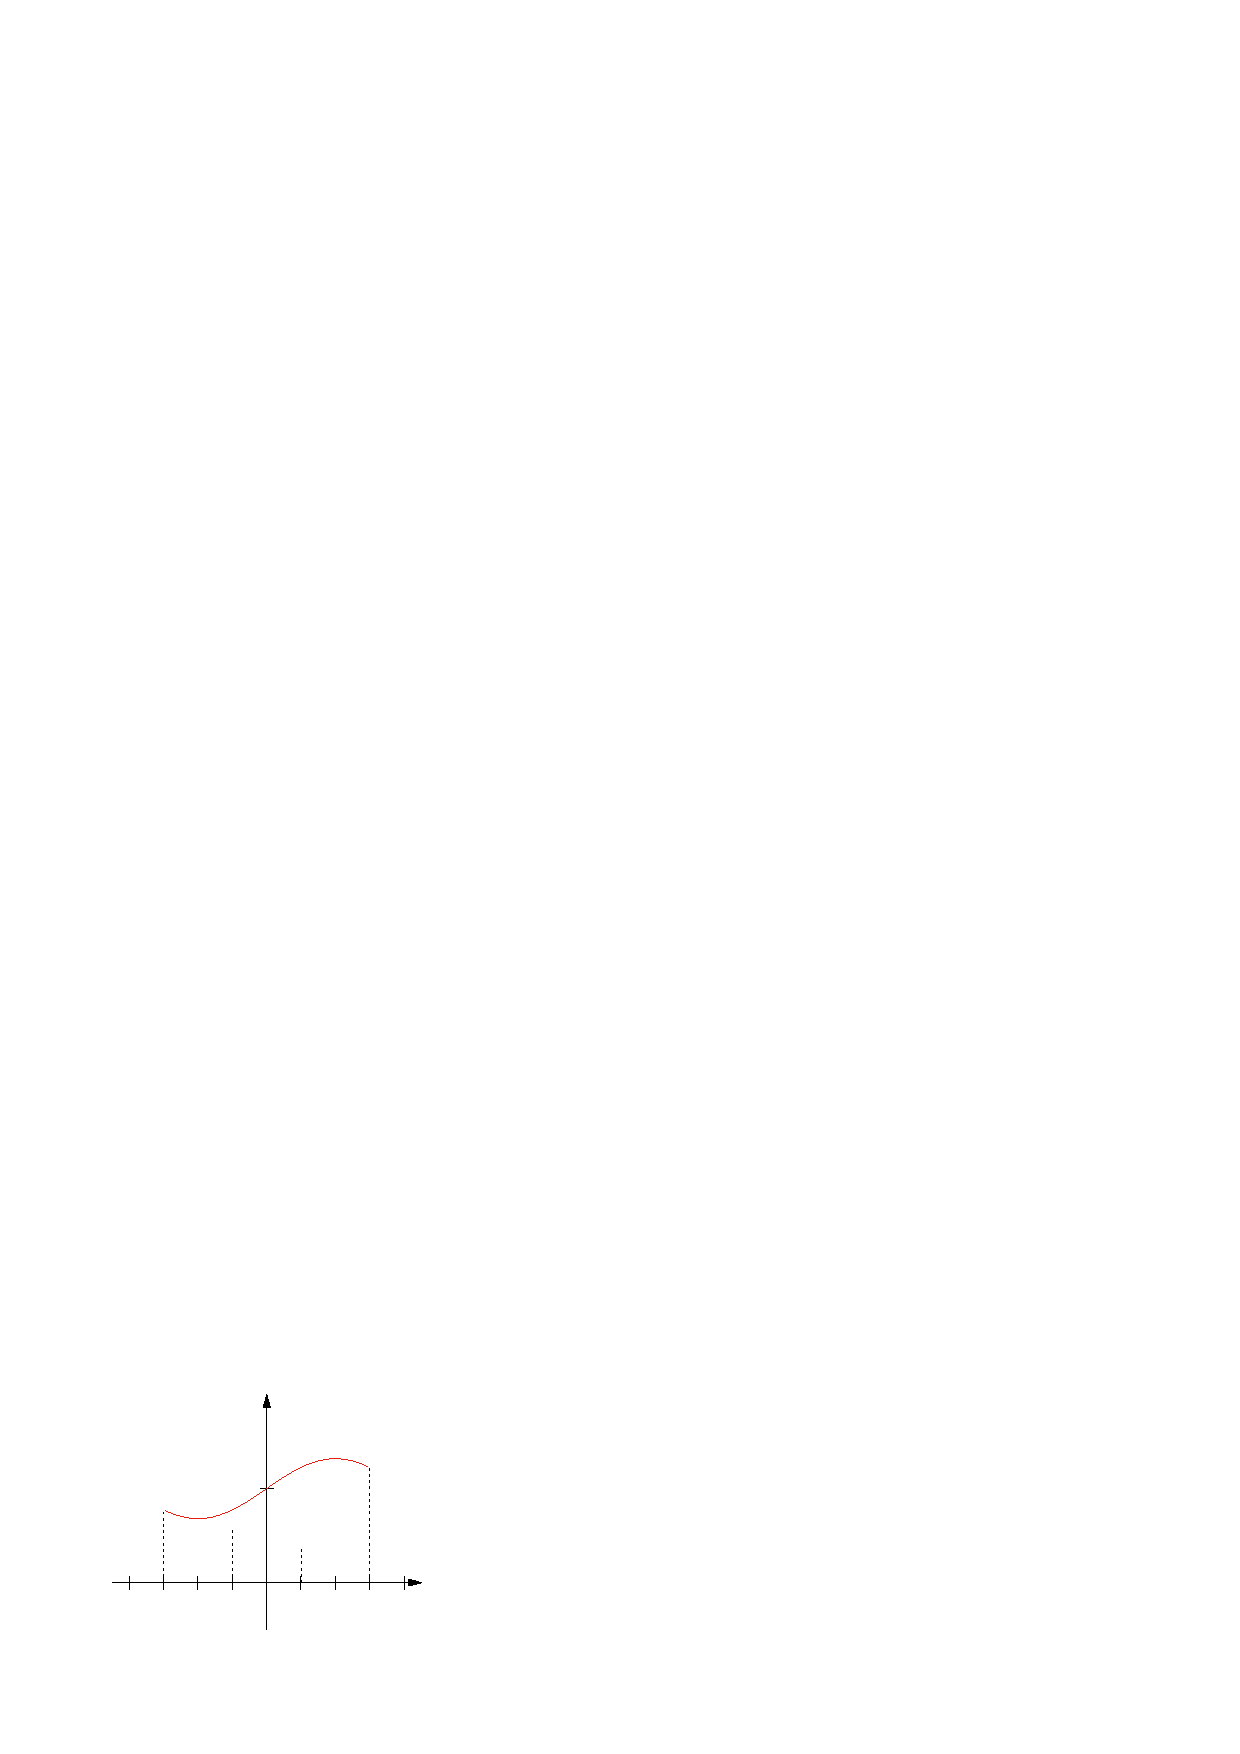
\includegraphics[width={158.40bp},height={108.00bp}]{figura_05_01}}%
    \gplfronttext
  \end{picture}%
\endgroup

    \end{minipage}
    \begin{minipage}{.4\textwidth}
        \centering
        % GNUPLOT: LaTeX picture with Postscript
\begingroup
  \makeatletter
  \providecommand\color[2][]{%
    \GenericError{(gnuplot) \space\space\space\@spaces}{%
      Package color not loaded in conjunction with
      terminal option `colourtext'%
    }{See the gnuplot documentation for explanation.%
    }{Either use 'blacktext' in gnuplot or load the package
      color.sty in LaTeX.}%
    \renewcommand\color[2][]{}%
  }%
  \providecommand\includegraphics[2][]{%
    \GenericError{(gnuplot) \space\space\space\@spaces}{%
      Package graphicx or graphics not loaded%
    }{See the gnuplot documentation for explanation.%
    }{The gnuplot epslatex terminal needs graphicx.sty or graphics.sty.}%
    \renewcommand\includegraphics[2][]{}%
  }%
  \providecommand\rotatebox[2]{#2}%
  \@ifundefined{ifGPcolor}{%
    \newif\ifGPcolor
    \GPcolorfalse
  }{}%
  \@ifundefined{ifGPblacktext}{%
    \newif\ifGPblacktext
    \GPblacktexttrue
  }{}%
  % define a \g@addto@macro without @ in the name:
  \let\gplgaddtomacro\g@addto@macro
  % define empty templates for all commands taking text:
  \gdef\gplbacktext{}%
  \gdef\gplfronttext{}%
  \makeatother
  \ifGPblacktext
    % no textcolor at all
    \def\colorrgb#1{}%
    \def\colorgray#1{}%
  \else
    % gray or color?
    \ifGPcolor
      \def\colorrgb#1{\color[rgb]{#1}}%
      \def\colorgray#1{\color[gray]{#1}}%
      \expandafter\def\csname LTw\endcsname{\color{white}}%
      \expandafter\def\csname LTb\endcsname{\color{black}}%
      \expandafter\def\csname LTa\endcsname{\color{black}}%
      \expandafter\def\csname LT0\endcsname{\color[rgb]{1,0,0}}%
      \expandafter\def\csname LT1\endcsname{\color[rgb]{0,1,0}}%
      \expandafter\def\csname LT2\endcsname{\color[rgb]{0,0,1}}%
      \expandafter\def\csname LT3\endcsname{\color[rgb]{1,0,1}}%
      \expandafter\def\csname LT4\endcsname{\color[rgb]{0,1,1}}%
      \expandafter\def\csname LT5\endcsname{\color[rgb]{1,1,0}}%
      \expandafter\def\csname LT6\endcsname{\color[rgb]{0,0,0}}%
      \expandafter\def\csname LT7\endcsname{\color[rgb]{1,0.3,0}}%
      \expandafter\def\csname LT8\endcsname{\color[rgb]{0.5,0.5,0.5}}%
    \else
      % gray
      \def\colorrgb#1{\color{black}}%
      \def\colorgray#1{\color[gray]{#1}}%
      \expandafter\def\csname LTw\endcsname{\color{white}}%
      \expandafter\def\csname LTb\endcsname{\color{black}}%
      \expandafter\def\csname LTa\endcsname{\color{black}}%
      \expandafter\def\csname LT0\endcsname{\color{black}}%
      \expandafter\def\csname LT1\endcsname{\color{black}}%
      \expandafter\def\csname LT2\endcsname{\color{black}}%
      \expandafter\def\csname LT3\endcsname{\color{black}}%
      \expandafter\def\csname LT4\endcsname{\color{black}}%
      \expandafter\def\csname LT5\endcsname{\color{black}}%
      \expandafter\def\csname LT6\endcsname{\color{black}}%
      \expandafter\def\csname LT7\endcsname{\color{black}}%
      \expandafter\def\csname LT8\endcsname{\color{black}}%
    \fi
  \fi
    \setlength{\unitlength}{0.0500bp}%
    \ifx\gptboxheight\undefined%
      \newlength{\gptboxheight}%
      \newlength{\gptboxwidth}%
      \newsavebox{\gptboxtext}%
    \fi%
    \setlength{\fboxrule}{0.5pt}%
    \setlength{\fboxsep}{1pt}%
    \definecolor{tbcol}{rgb}{1,1,1}%
\begin{picture}(3168.00,2160.00)%
    \gplgaddtomacro\gplbacktext{%
      \csname LTb\endcsname%%
      \put(1200,644){\makebox(0,0)[r]{\strut{}}}%
      \put(1200,1547){\makebox(0,0)[r]{\strut{}}}%
      \put(240,421){\makebox(0,0){\strut{}}}%
      \put(504,421){\makebox(0,0){\strut{}}}%
      \put(768,421){\makebox(0,0){\strut{}}}%
      \put(1032,421){\makebox(0,0){\strut{}}}%
      \put(1296,421){\makebox(0,0){\strut{}}}%
      \put(1560,421){\makebox(0,0){\strut{}}}%
      \put(1823,421){\makebox(0,0){\strut{}}}%
      \put(2087,421){\makebox(0,0){\strut{}}}%
      \put(2351,421){\makebox(0,0){\strut{}}}%
      \put(2615,421){\makebox(0,0){\strut{}}}%
      \put(2879,421){\makebox(0,0){\strut{}}}%
      \csname LTb\endcsname%%
      \put(3064,644){\makebox(0,0)[l]{\strut{}$t$}}%
      \put(834,2270){\makebox(0,0)[l]{\strut{}$f(\tau)$}}%
      \put(1678,1999){\makebox(0,0)[l]{\strut{}$f_1(\tau)$}}%
      \put(1084,1367){\makebox(0,0)[l]{\strut{}$f_2(-\tau)$}}%
      \put(2444,1367){\makebox(0,0)[l]{\strut{}$f_2(t-\tau)$}}%
      \put(1459,212){\makebox(0,0)[l]{\strut{}$t$}}%
    }%
    \gplgaddtomacro\gplfronttext{%
    }%
    \gplgaddtomacro\gplbacktext{%
      \csname LTb\endcsname%%
      \put(1200,644){\makebox(0,0)[r]{\strut{}}}%
      \put(1200,1547){\makebox(0,0)[r]{\strut{}}}%
      \put(240,421){\makebox(0,0){\strut{}}}%
      \put(504,421){\makebox(0,0){\strut{}}}%
      \put(768,421){\makebox(0,0){\strut{}}}%
      \put(1032,421){\makebox(0,0){\strut{}}}%
      \put(1296,421){\makebox(0,0){\strut{}}}%
      \put(1560,421){\makebox(0,0){\strut{}}}%
      \put(1823,421){\makebox(0,0){\strut{}}}%
      \put(2087,421){\makebox(0,0){\strut{}}}%
      \put(2351,421){\makebox(0,0){\strut{}}}%
      \put(2615,421){\makebox(0,0){\strut{}}}%
      \put(2879,421){\makebox(0,0){\strut{}}}%
      \csname LTb\endcsname%%
      \put(3064,644){\makebox(0,0)[l]{\strut{}$t$}}%
      \put(834,2270){\makebox(0,0)[l]{\strut{}$f(\tau)$}}%
      \put(1678,1999){\makebox(0,0)[l]{\strut{}$f_1(\tau)$}}%
      \put(1084,1367){\makebox(0,0)[l]{\strut{}$f_2(-\tau)$}}%
      \put(2444,1367){\makebox(0,0)[l]{\strut{}$f_2(t-\tau)$}}%
      \put(1459,212){\makebox(0,0)[l]{\strut{}$t$}}%
    }%
    \gplgaddtomacro\gplfronttext{%
    }%
    \gplgaddtomacro\gplbacktext{%
      \csname LTb\endcsname%%
      \put(1200,644){\makebox(0,0)[r]{\strut{}}}%
      \put(1200,1547){\makebox(0,0)[r]{\strut{}}}%
      \put(240,421){\makebox(0,0){\strut{}}}%
      \put(504,421){\makebox(0,0){\strut{}}}%
      \put(768,421){\makebox(0,0){\strut{}}}%
      \put(1032,421){\makebox(0,0){\strut{}}}%
      \put(1296,421){\makebox(0,0){\strut{}}}%
      \put(1560,421){\makebox(0,0){\strut{}}}%
      \put(1823,421){\makebox(0,0){\strut{}}}%
      \put(2087,421){\makebox(0,0){\strut{}}}%
      \put(2351,421){\makebox(0,0){\strut{}}}%
      \put(2615,421){\makebox(0,0){\strut{}}}%
      \put(2879,421){\makebox(0,0){\strut{}}}%
      \csname LTb\endcsname%%
      \put(3064,644){\makebox(0,0)[l]{\strut{}$t$}}%
      \put(834,2270){\makebox(0,0)[l]{\strut{}$f(\tau)$}}%
      \put(1678,1999){\makebox(0,0)[l]{\strut{}$f_1(\tau)$}}%
      \put(1084,1367){\makebox(0,0)[l]{\strut{}$f_2(-\tau)$}}%
      \put(2444,1367){\makebox(0,0)[l]{\strut{}$f_2(t-\tau)$}}%
      \put(1459,212){\makebox(0,0)[l]{\strut{}$t$}}%
    }%
    \gplgaddtomacro\gplfronttext{%
    }%
    \gplgaddtomacro\gplbacktext{%
      \csname LTb\endcsname%%
      \put(1200,644){\makebox(0,0)[r]{\strut{}}}%
      \put(1200,1547){\makebox(0,0)[r]{\strut{}}}%
      \put(240,421){\makebox(0,0){\strut{}}}%
      \put(504,421){\makebox(0,0){\strut{}}}%
      \put(768,421){\makebox(0,0){\strut{}}}%
      \put(1032,421){\makebox(0,0){\strut{}}}%
      \put(1296,421){\makebox(0,0){\strut{}}}%
      \put(1560,421){\makebox(0,0){\strut{}}}%
      \put(1823,421){\makebox(0,0){\strut{}}}%
      \put(2087,421){\makebox(0,0){\strut{}}}%
      \put(2351,421){\makebox(0,0){\strut{}}}%
      \put(2615,421){\makebox(0,0){\strut{}}}%
      \put(2879,421){\makebox(0,0){\strut{}}}%
      \csname LTb\endcsname%%
      \put(3064,644){\makebox(0,0)[l]{\strut{}$t$}}%
      \put(834,2270){\makebox(0,0)[l]{\strut{}$f(\tau)$}}%
      \put(1678,1999){\makebox(0,0)[l]{\strut{}$f_1(\tau)$}}%
      \put(1084,1367){\makebox(0,0)[l]{\strut{}$f_2(-\tau)$}}%
      \put(2444,1367){\makebox(0,0)[l]{\strut{}$f_2(t-\tau)$}}%
      \put(1459,212){\makebox(0,0)[l]{\strut{}$t$}}%
    }%
    \gplgaddtomacro\gplfronttext{%
    }%
    \gplgaddtomacro\gplbacktext{%
      \csname LTb\endcsname%%
      \put(1200,644){\makebox(0,0)[r]{\strut{}}}%
      \put(1200,1547){\makebox(0,0)[r]{\strut{}}}%
      \put(240,421){\makebox(0,0){\strut{}}}%
      \put(504,421){\makebox(0,0){\strut{}}}%
      \put(768,421){\makebox(0,0){\strut{}}}%
      \put(1032,421){\makebox(0,0){\strut{}}}%
      \put(1296,421){\makebox(0,0){\strut{}}}%
      \put(1560,421){\makebox(0,0){\strut{}}}%
      \put(1823,421){\makebox(0,0){\strut{}}}%
      \put(2087,421){\makebox(0,0){\strut{}}}%
      \put(2351,421){\makebox(0,0){\strut{}}}%
      \put(2615,421){\makebox(0,0){\strut{}}}%
      \put(2879,421){\makebox(0,0){\strut{}}}%
      \csname LTb\endcsname%%
      \put(3064,644){\makebox(0,0)[l]{\strut{}$t$}}%
      \put(834,2270){\makebox(0,0)[l]{\strut{}$f(\tau)$}}%
      \put(1678,1999){\makebox(0,0)[l]{\strut{}$f_1(\tau)$}}%
      \put(1084,1367){\makebox(0,0)[l]{\strut{}$f_2(-\tau)$}}%
      \put(2444,1367){\makebox(0,0)[l]{\strut{}$f_2(t-\tau)$}}%
      \put(1459,212){\makebox(0,0)[l]{\strut{}$t$}}%
    }%
    \gplgaddtomacro\gplfronttext{%
    }%
    \gplbacktext
    \put(0,0){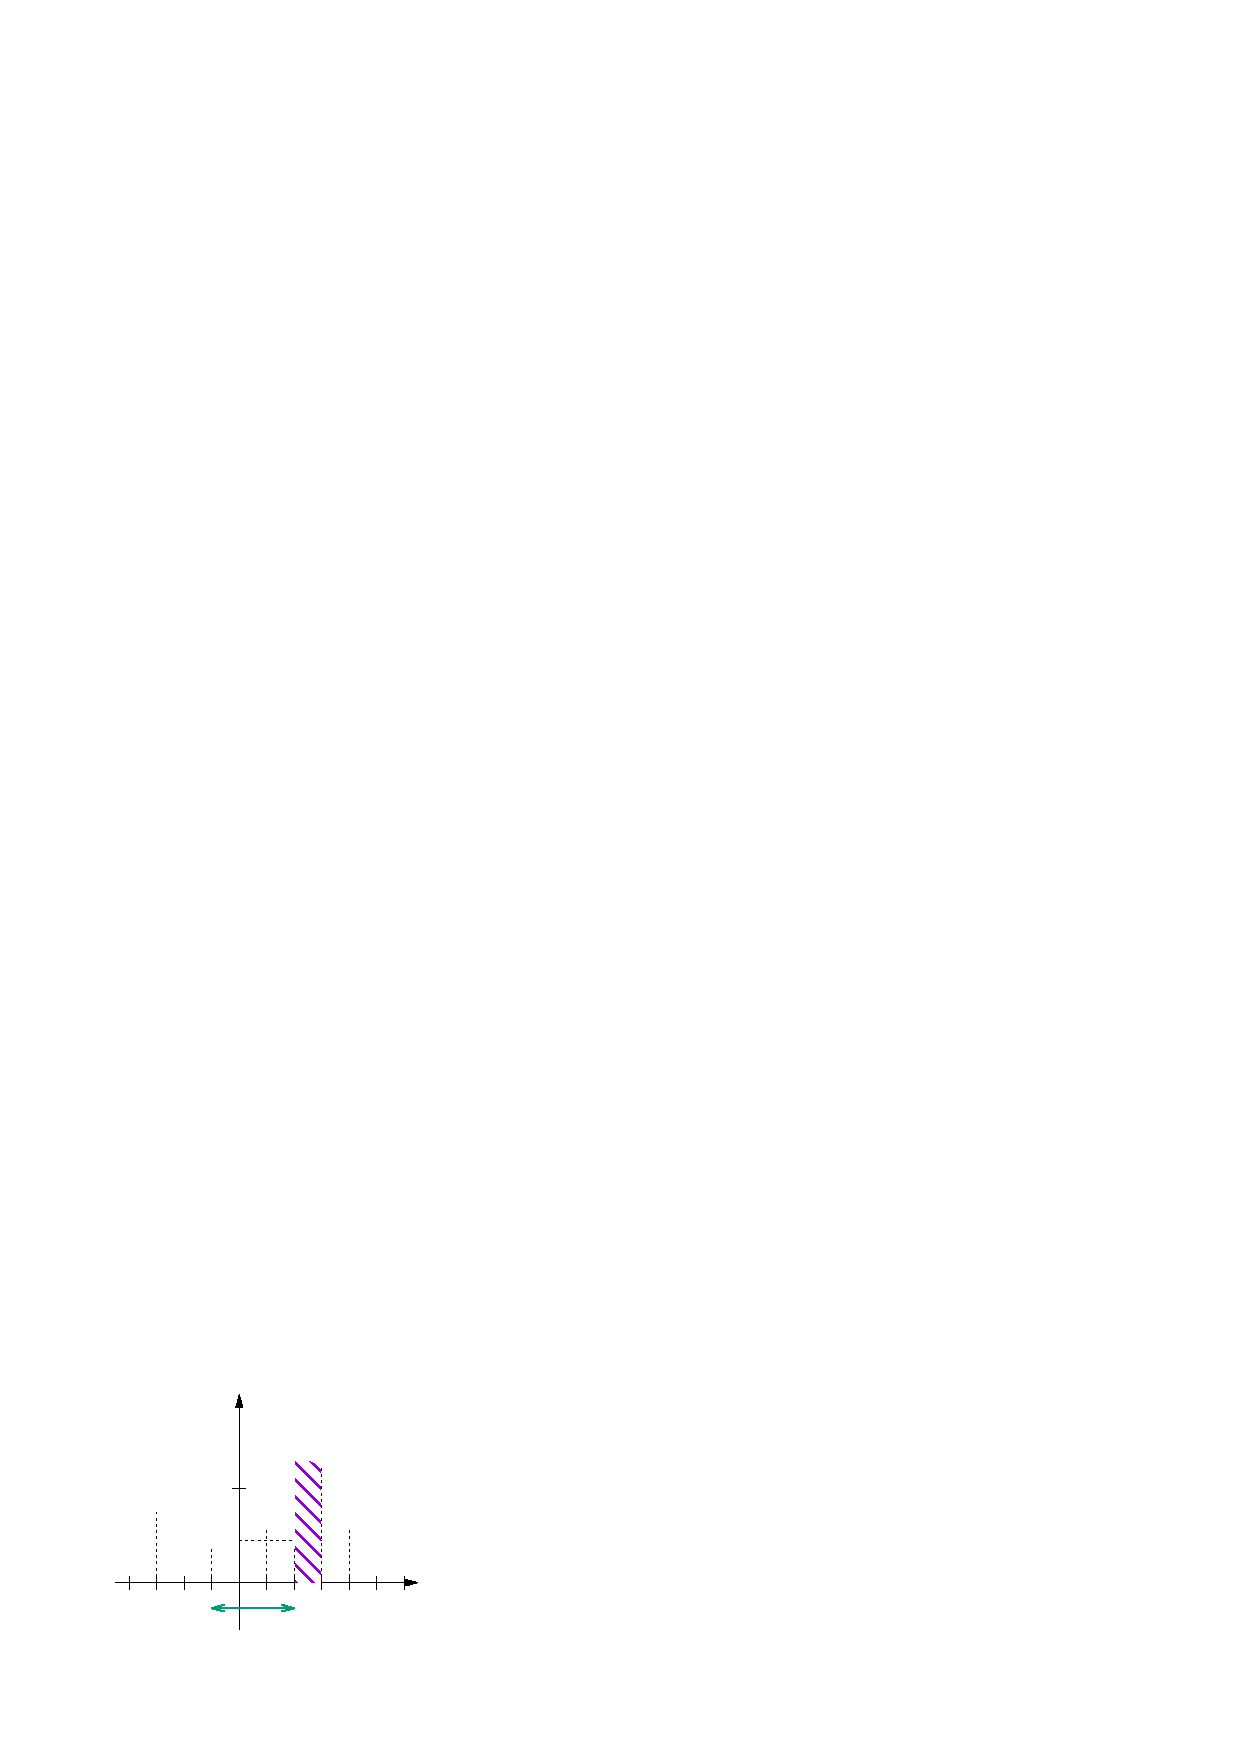
\includegraphics[width={158.40bp},height={108.00bp}]{figura_05_02}}%
    \gplfronttext
  \end{picture}%
\endgroup

    \end{minipage}
\end{figure}
El intervalo de integración será el intervalo donde ambas gráficas se
superponen.

\section{Propiedades de la convolución}

\subsection{Conmutatividad}
\begin{equation}
    f_1(t)*f_2(t)=f_2(t)*f_1(t)
\end{equation}

\subsection{Asociatividad}
\begin{equation}
    f_1(t)*[f_2(t)*f_3(t)]=[f_1(t)*f_2(t)]*f_3(t)
\end{equation}

\subsection{Distributividad}
\begin{equation}
    f_1(t)*[f_2(t)+f_3(t)]=f_1(t)*f_2(t)+f_1(t)*f_3(t)
\end{equation}

\subsection{Función impulso}
\begin{equation}
    f_1(t)*\delta(t-t_0)=f_1(t-t_0)
\end{equation}

\underline{Prueba}:

\begin{equation*}
    f_1(t)*\delta(t-t_0)
    =\int_{-\infty}^{\infty}\,f_1(t-\tau)\,\delta(\tau-t_0)\,d\tau
    =f_1(t-t_0)
\end{equation*}

\subsection{Función escalón unitario}
Si $f_1(t)=f_1(t)\,u(t)$ y $f_2(t)=f_2(t)\,u(t)$:
\begin{equation}
    f_1(t)*f_2(t)=\int_0^t\,f_1(\tau)\,f_2(t-\tau)\,d\tau
\end{equation}

\begin{figure}[H]
    \centering
    \begin{minipage}{.4\textwidth}
        \centering
        % GNUPLOT: LaTeX picture with Postscript
\begingroup
  \makeatletter
  \providecommand\color[2][]{%
    \GenericError{(gnuplot) \space\space\space\@spaces}{%
      Package color not loaded in conjunction with
      terminal option `colourtext'%
    }{See the gnuplot documentation for explanation.%
    }{Either use 'blacktext' in gnuplot or load the package
      color.sty in LaTeX.}%
    \renewcommand\color[2][]{}%
  }%
  \providecommand\includegraphics[2][]{%
    \GenericError{(gnuplot) \space\space\space\@spaces}{%
      Package graphicx or graphics not loaded%
    }{See the gnuplot documentation for explanation.%
    }{The gnuplot epslatex terminal needs graphicx.sty or graphics.sty.}%
    \renewcommand\includegraphics[2][]{}%
  }%
  \providecommand\rotatebox[2]{#2}%
  \@ifundefined{ifGPcolor}{%
    \newif\ifGPcolor
    \GPcolorfalse
  }{}%
  \@ifundefined{ifGPblacktext}{%
    \newif\ifGPblacktext
    \GPblacktexttrue
  }{}%
  % define a \g@addto@macro without @ in the name:
  \let\gplgaddtomacro\g@addto@macro
  % define empty templates for all commands taking text:
  \gdef\gplbacktext{}%
  \gdef\gplfronttext{}%
  \makeatother
  \ifGPblacktext
    % no textcolor at all
    \def\colorrgb#1{}%
    \def\colorgray#1{}%
  \else
    % gray or color?
    \ifGPcolor
      \def\colorrgb#1{\color[rgb]{#1}}%
      \def\colorgray#1{\color[gray]{#1}}%
      \expandafter\def\csname LTw\endcsname{\color{white}}%
      \expandafter\def\csname LTb\endcsname{\color{black}}%
      \expandafter\def\csname LTa\endcsname{\color{black}}%
      \expandafter\def\csname LT0\endcsname{\color[rgb]{1,0,0}}%
      \expandafter\def\csname LT1\endcsname{\color[rgb]{0,1,0}}%
      \expandafter\def\csname LT2\endcsname{\color[rgb]{0,0,1}}%
      \expandafter\def\csname LT3\endcsname{\color[rgb]{1,0,1}}%
      \expandafter\def\csname LT4\endcsname{\color[rgb]{0,1,1}}%
      \expandafter\def\csname LT5\endcsname{\color[rgb]{1,1,0}}%
      \expandafter\def\csname LT6\endcsname{\color[rgb]{0,0,0}}%
      \expandafter\def\csname LT7\endcsname{\color[rgb]{1,0.3,0}}%
      \expandafter\def\csname LT8\endcsname{\color[rgb]{0.5,0.5,0.5}}%
    \else
      % gray
      \def\colorrgb#1{\color{black}}%
      \def\colorgray#1{\color[gray]{#1}}%
      \expandafter\def\csname LTw\endcsname{\color{white}}%
      \expandafter\def\csname LTb\endcsname{\color{black}}%
      \expandafter\def\csname LTa\endcsname{\color{black}}%
      \expandafter\def\csname LT0\endcsname{\color{black}}%
      \expandafter\def\csname LT1\endcsname{\color{black}}%
      \expandafter\def\csname LT2\endcsname{\color{black}}%
      \expandafter\def\csname LT3\endcsname{\color{black}}%
      \expandafter\def\csname LT4\endcsname{\color{black}}%
      \expandafter\def\csname LT5\endcsname{\color{black}}%
      \expandafter\def\csname LT6\endcsname{\color{black}}%
      \expandafter\def\csname LT7\endcsname{\color{black}}%
      \expandafter\def\csname LT8\endcsname{\color{black}}%
    \fi
  \fi
    \setlength{\unitlength}{0.0500bp}%
    \ifx\gptboxheight\undefined%
      \newlength{\gptboxheight}%
      \newlength{\gptboxwidth}%
      \newsavebox{\gptboxtext}%
    \fi%
    \setlength{\fboxrule}{0.5pt}%
    \setlength{\fboxsep}{1pt}%
    \definecolor{tbcol}{rgb}{1,1,1}%
\begin{picture}(3168.00,2160.00)%
    \gplgaddtomacro\gplbacktext{%
      \csname LTb\endcsname%%
      \put(437,644){\makebox(0,0)[r]{\strut{}}}%
      \put(437,1547){\makebox(0,0)[r]{\strut{}}}%
      \put(533,421){\makebox(0,0){\strut{}}}%
      \put(1120,421){\makebox(0,0){\strut{}}}%
      \put(1706,421){\makebox(0,0){\strut{}}}%
      \put(2293,421){\makebox(0,0){\strut{}}}%
      \put(2879,421){\makebox(0,0){\strut{}}}%
      \csname LTb\endcsname%%
      \put(3290,644){\makebox(0,0)[l]{\strut{}$t$}}%
      \put(5,2360){\makebox(0,0)[l]{\strut{}$f(t)$}}%
      \put(1384,1999){\makebox(0,0)[l]{\strut{}$f_1(t)$}}%
      \put(1120,1276){\makebox(0,0)[l]{\strut{}$f_2(t)$}}%
    }%
    \gplgaddtomacro\gplfronttext{%
    }%
    \gplgaddtomacro\gplbacktext{%
      \csname LTb\endcsname%%
      \put(437,644){\makebox(0,0)[r]{\strut{}}}%
      \put(437,1547){\makebox(0,0)[r]{\strut{}}}%
      \put(533,421){\makebox(0,0){\strut{}}}%
      \put(1120,421){\makebox(0,0){\strut{}}}%
      \put(1706,421){\makebox(0,0){\strut{}}}%
      \put(2293,421){\makebox(0,0){\strut{}}}%
      \put(2879,421){\makebox(0,0){\strut{}}}%
      \csname LTb\endcsname%%
      \put(3290,644){\makebox(0,0)[l]{\strut{}$t$}}%
      \put(5,2360){\makebox(0,0)[l]{\strut{}$f(t)$}}%
      \put(1384,1999){\makebox(0,0)[l]{\strut{}$f_1(t)$}}%
      \put(1120,1276){\makebox(0,0)[l]{\strut{}$f_2(t)$}}%
    }%
    \gplgaddtomacro\gplfronttext{%
    }%
    \gplbacktext
    \put(0,0){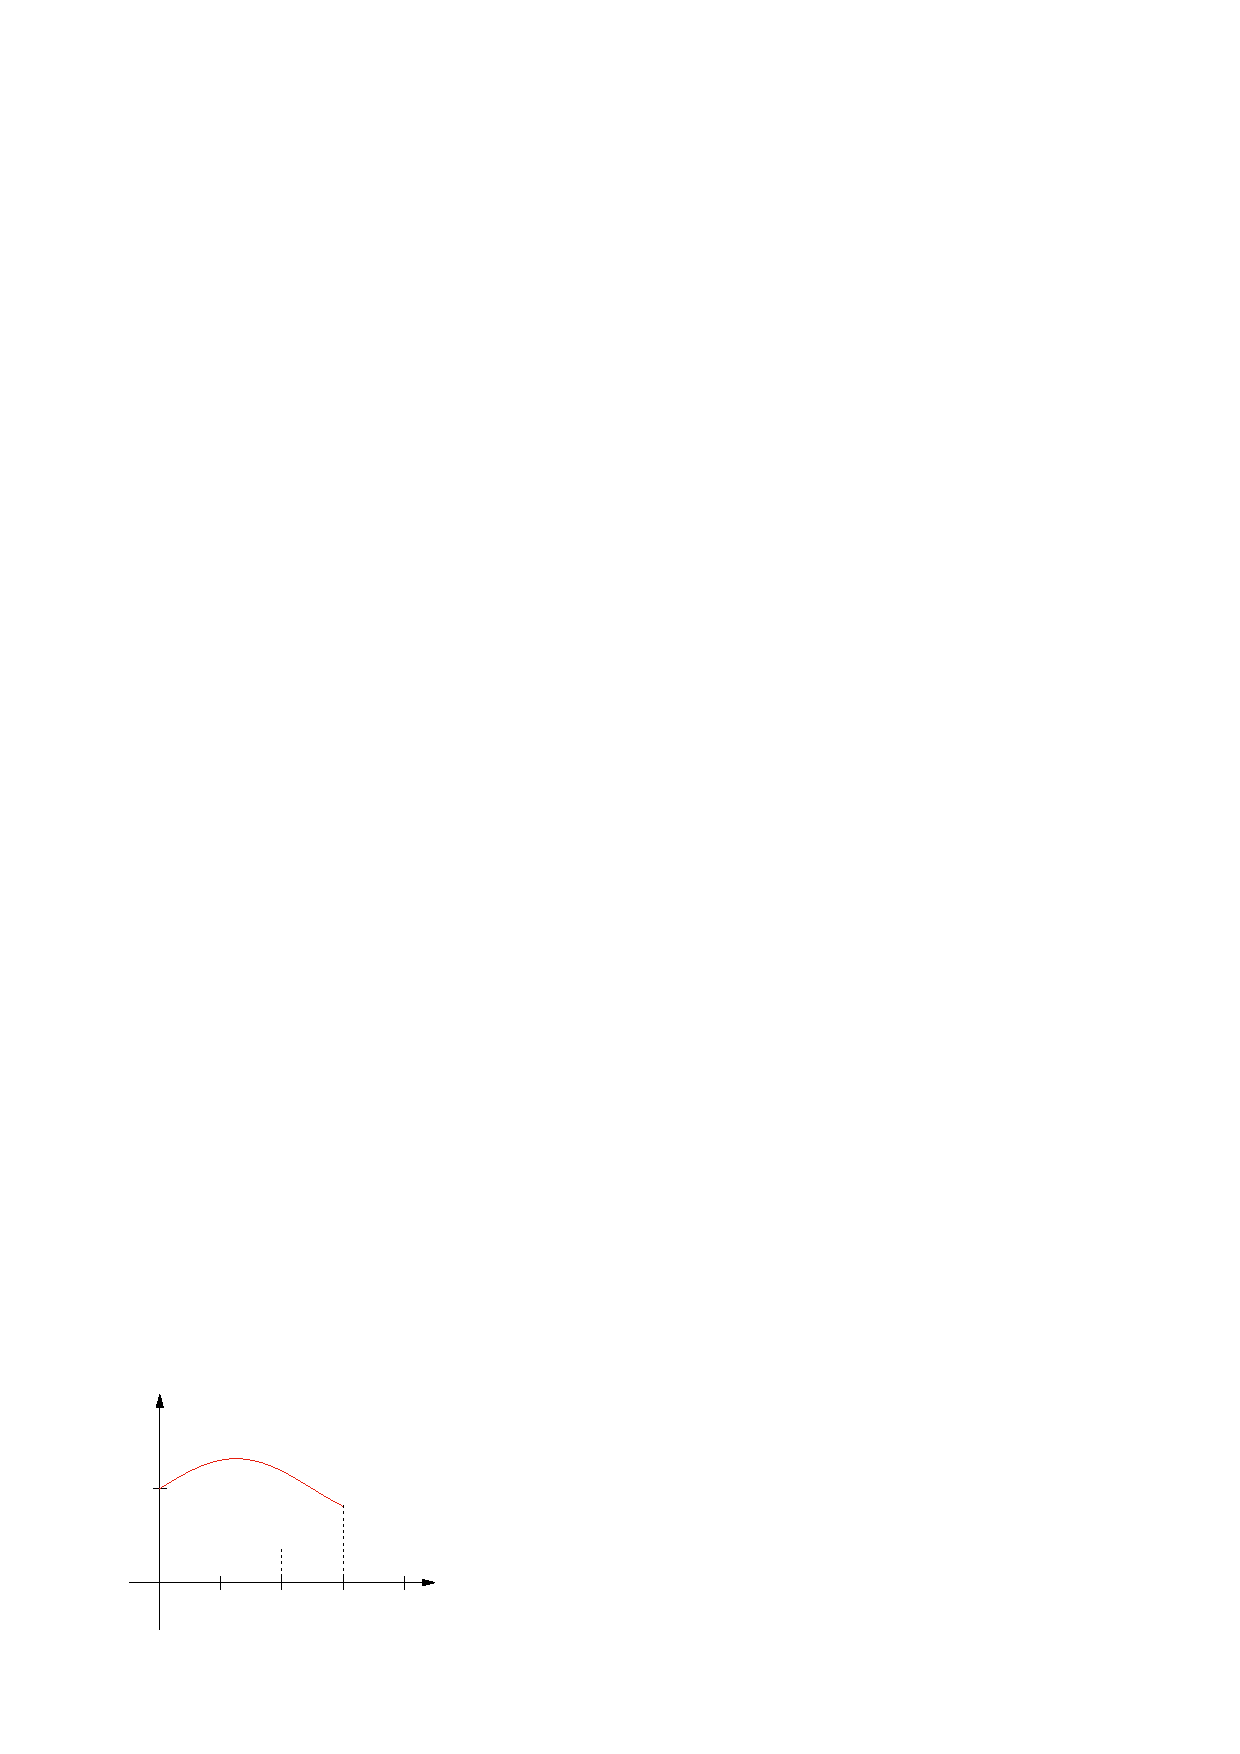
\includegraphics[width={158.40bp},height={108.00bp}]{figura_05_03}}%
    \gplfronttext
  \end{picture}%
\endgroup

    \end{minipage}
    \begin{minipage}{.4\textwidth}
        \centering
        % GNUPLOT: LaTeX picture with Postscript
\begingroup
  \makeatletter
  \providecommand\color[2][]{%
    \GenericError{(gnuplot) \space\space\space\@spaces}{%
      Package color not loaded in conjunction with
      terminal option `colourtext'%
    }{See the gnuplot documentation for explanation.%
    }{Either use 'blacktext' in gnuplot or load the package
      color.sty in LaTeX.}%
    \renewcommand\color[2][]{}%
  }%
  \providecommand\includegraphics[2][]{%
    \GenericError{(gnuplot) \space\space\space\@spaces}{%
      Package graphicx or graphics not loaded%
    }{See the gnuplot documentation for explanation.%
    }{The gnuplot epslatex terminal needs graphicx.sty or graphics.sty.}%
    \renewcommand\includegraphics[2][]{}%
  }%
  \providecommand\rotatebox[2]{#2}%
  \@ifundefined{ifGPcolor}{%
    \newif\ifGPcolor
    \GPcolorfalse
  }{}%
  \@ifundefined{ifGPblacktext}{%
    \newif\ifGPblacktext
    \GPblacktexttrue
  }{}%
  % define a \g@addto@macro without @ in the name:
  \let\gplgaddtomacro\g@addto@macro
  % define empty templates for all commands taking text:
  \gdef\gplbacktext{}%
  \gdef\gplfronttext{}%
  \makeatother
  \ifGPblacktext
    % no textcolor at all
    \def\colorrgb#1{}%
    \def\colorgray#1{}%
  \else
    % gray or color?
    \ifGPcolor
      \def\colorrgb#1{\color[rgb]{#1}}%
      \def\colorgray#1{\color[gray]{#1}}%
      \expandafter\def\csname LTw\endcsname{\color{white}}%
      \expandafter\def\csname LTb\endcsname{\color{black}}%
      \expandafter\def\csname LTa\endcsname{\color{black}}%
      \expandafter\def\csname LT0\endcsname{\color[rgb]{1,0,0}}%
      \expandafter\def\csname LT1\endcsname{\color[rgb]{0,1,0}}%
      \expandafter\def\csname LT2\endcsname{\color[rgb]{0,0,1}}%
      \expandafter\def\csname LT3\endcsname{\color[rgb]{1,0,1}}%
      \expandafter\def\csname LT4\endcsname{\color[rgb]{0,1,1}}%
      \expandafter\def\csname LT5\endcsname{\color[rgb]{1,1,0}}%
      \expandafter\def\csname LT6\endcsname{\color[rgb]{0,0,0}}%
      \expandafter\def\csname LT7\endcsname{\color[rgb]{1,0.3,0}}%
      \expandafter\def\csname LT8\endcsname{\color[rgb]{0.5,0.5,0.5}}%
    \else
      % gray
      \def\colorrgb#1{\color{black}}%
      \def\colorgray#1{\color[gray]{#1}}%
      \expandafter\def\csname LTw\endcsname{\color{white}}%
      \expandafter\def\csname LTb\endcsname{\color{black}}%
      \expandafter\def\csname LTa\endcsname{\color{black}}%
      \expandafter\def\csname LT0\endcsname{\color{black}}%
      \expandafter\def\csname LT1\endcsname{\color{black}}%
      \expandafter\def\csname LT2\endcsname{\color{black}}%
      \expandafter\def\csname LT3\endcsname{\color{black}}%
      \expandafter\def\csname LT4\endcsname{\color{black}}%
      \expandafter\def\csname LT5\endcsname{\color{black}}%
      \expandafter\def\csname LT6\endcsname{\color{black}}%
      \expandafter\def\csname LT7\endcsname{\color{black}}%
      \expandafter\def\csname LT8\endcsname{\color{black}}%
    \fi
  \fi
    \setlength{\unitlength}{0.0500bp}%
    \ifx\gptboxheight\undefined%
      \newlength{\gptboxheight}%
      \newlength{\gptboxwidth}%
      \newsavebox{\gptboxtext}%
    \fi%
    \setlength{\fboxrule}{0.5pt}%
    \setlength{\fboxsep}{1pt}%
    \definecolor{tbcol}{rgb}{1,1,1}%
\begin{picture}(3168.00,2160.00)%
    \gplgaddtomacro\gplbacktext{%
      \csname LTb\endcsname%%
      \put(437,644){\makebox(0,0)[r]{\strut{}}}%
      \put(437,1547){\makebox(0,0)[r]{\strut{}}}%
      \put(533,421){\makebox(0,0){\strut{}}}%
      \put(1120,421){\makebox(0,0){\strut{}}}%
      \put(1706,421){\makebox(0,0){\strut{}}}%
      \put(2293,421){\makebox(0,0){\strut{}}}%
      \put(2879,421){\makebox(0,0){\strut{}}}%
      \csname LTb\endcsname%%
      \put(3290,644){\makebox(0,0)[l]{\strut{}$t$}}%
      \put(5,2360){\makebox(0,0)[l]{\strut{}$f(\tau)$}}%
      \put(1384,1999){\makebox(0,0)[l]{\strut{}$f_1(\tau)$}}%
      \put(1237,1276){\makebox(0,0)[l]{\strut{}$f_2(t-\tau)$}}%
      \put(1061,428){\makebox(0,0)[l]{\strut{}$t$}}%
    }%
    \gplgaddtomacro\gplfronttext{%
    }%
    \gplgaddtomacro\gplbacktext{%
      \csname LTb\endcsname%%
      \put(437,644){\makebox(0,0)[r]{\strut{}}}%
      \put(437,1547){\makebox(0,0)[r]{\strut{}}}%
      \put(533,421){\makebox(0,0){\strut{}}}%
      \put(1120,421){\makebox(0,0){\strut{}}}%
      \put(1706,421){\makebox(0,0){\strut{}}}%
      \put(2293,421){\makebox(0,0){\strut{}}}%
      \put(2879,421){\makebox(0,0){\strut{}}}%
      \csname LTb\endcsname%%
      \put(3290,644){\makebox(0,0)[l]{\strut{}$t$}}%
      \put(5,2360){\makebox(0,0)[l]{\strut{}$f(\tau)$}}%
      \put(1384,1999){\makebox(0,0)[l]{\strut{}$f_1(\tau)$}}%
      \put(1237,1276){\makebox(0,0)[l]{\strut{}$f_2(t-\tau)$}}%
      \put(1061,428){\makebox(0,0)[l]{\strut{}$t$}}%
    }%
    \gplgaddtomacro\gplfronttext{%
    }%
    \gplgaddtomacro\gplbacktext{%
      \csname LTb\endcsname%%
      \put(437,644){\makebox(0,0)[r]{\strut{}}}%
      \put(437,1547){\makebox(0,0)[r]{\strut{}}}%
      \put(533,421){\makebox(0,0){\strut{}}}%
      \put(1120,421){\makebox(0,0){\strut{}}}%
      \put(1706,421){\makebox(0,0){\strut{}}}%
      \put(2293,421){\makebox(0,0){\strut{}}}%
      \put(2879,421){\makebox(0,0){\strut{}}}%
      \csname LTb\endcsname%%
      \put(3290,644){\makebox(0,0)[l]{\strut{}$t$}}%
      \put(5,2360){\makebox(0,0)[l]{\strut{}$f(\tau)$}}%
      \put(1384,1999){\makebox(0,0)[l]{\strut{}$f_1(\tau)$}}%
      \put(1237,1276){\makebox(0,0)[l]{\strut{}$f_2(t-\tau)$}}%
      \put(1061,428){\makebox(0,0)[l]{\strut{}$t$}}%
    }%
    \gplgaddtomacro\gplfronttext{%
    }%
    \gplgaddtomacro\gplbacktext{%
      \csname LTb\endcsname%%
      \put(437,644){\makebox(0,0)[r]{\strut{}}}%
      \put(437,1547){\makebox(0,0)[r]{\strut{}}}%
      \put(533,421){\makebox(0,0){\strut{}}}%
      \put(1120,421){\makebox(0,0){\strut{}}}%
      \put(1706,421){\makebox(0,0){\strut{}}}%
      \put(2293,421){\makebox(0,0){\strut{}}}%
      \put(2879,421){\makebox(0,0){\strut{}}}%
      \csname LTb\endcsname%%
      \put(3290,644){\makebox(0,0)[l]{\strut{}$t$}}%
      \put(5,2360){\makebox(0,0)[l]{\strut{}$f(\tau)$}}%
      \put(1384,1999){\makebox(0,0)[l]{\strut{}$f_1(\tau)$}}%
      \put(1237,1276){\makebox(0,0)[l]{\strut{}$f_2(t-\tau)$}}%
      \put(1061,428){\makebox(0,0)[l]{\strut{}$t$}}%
    }%
    \gplgaddtomacro\gplfronttext{%
    }%
    \gplbacktext
    \put(0,0){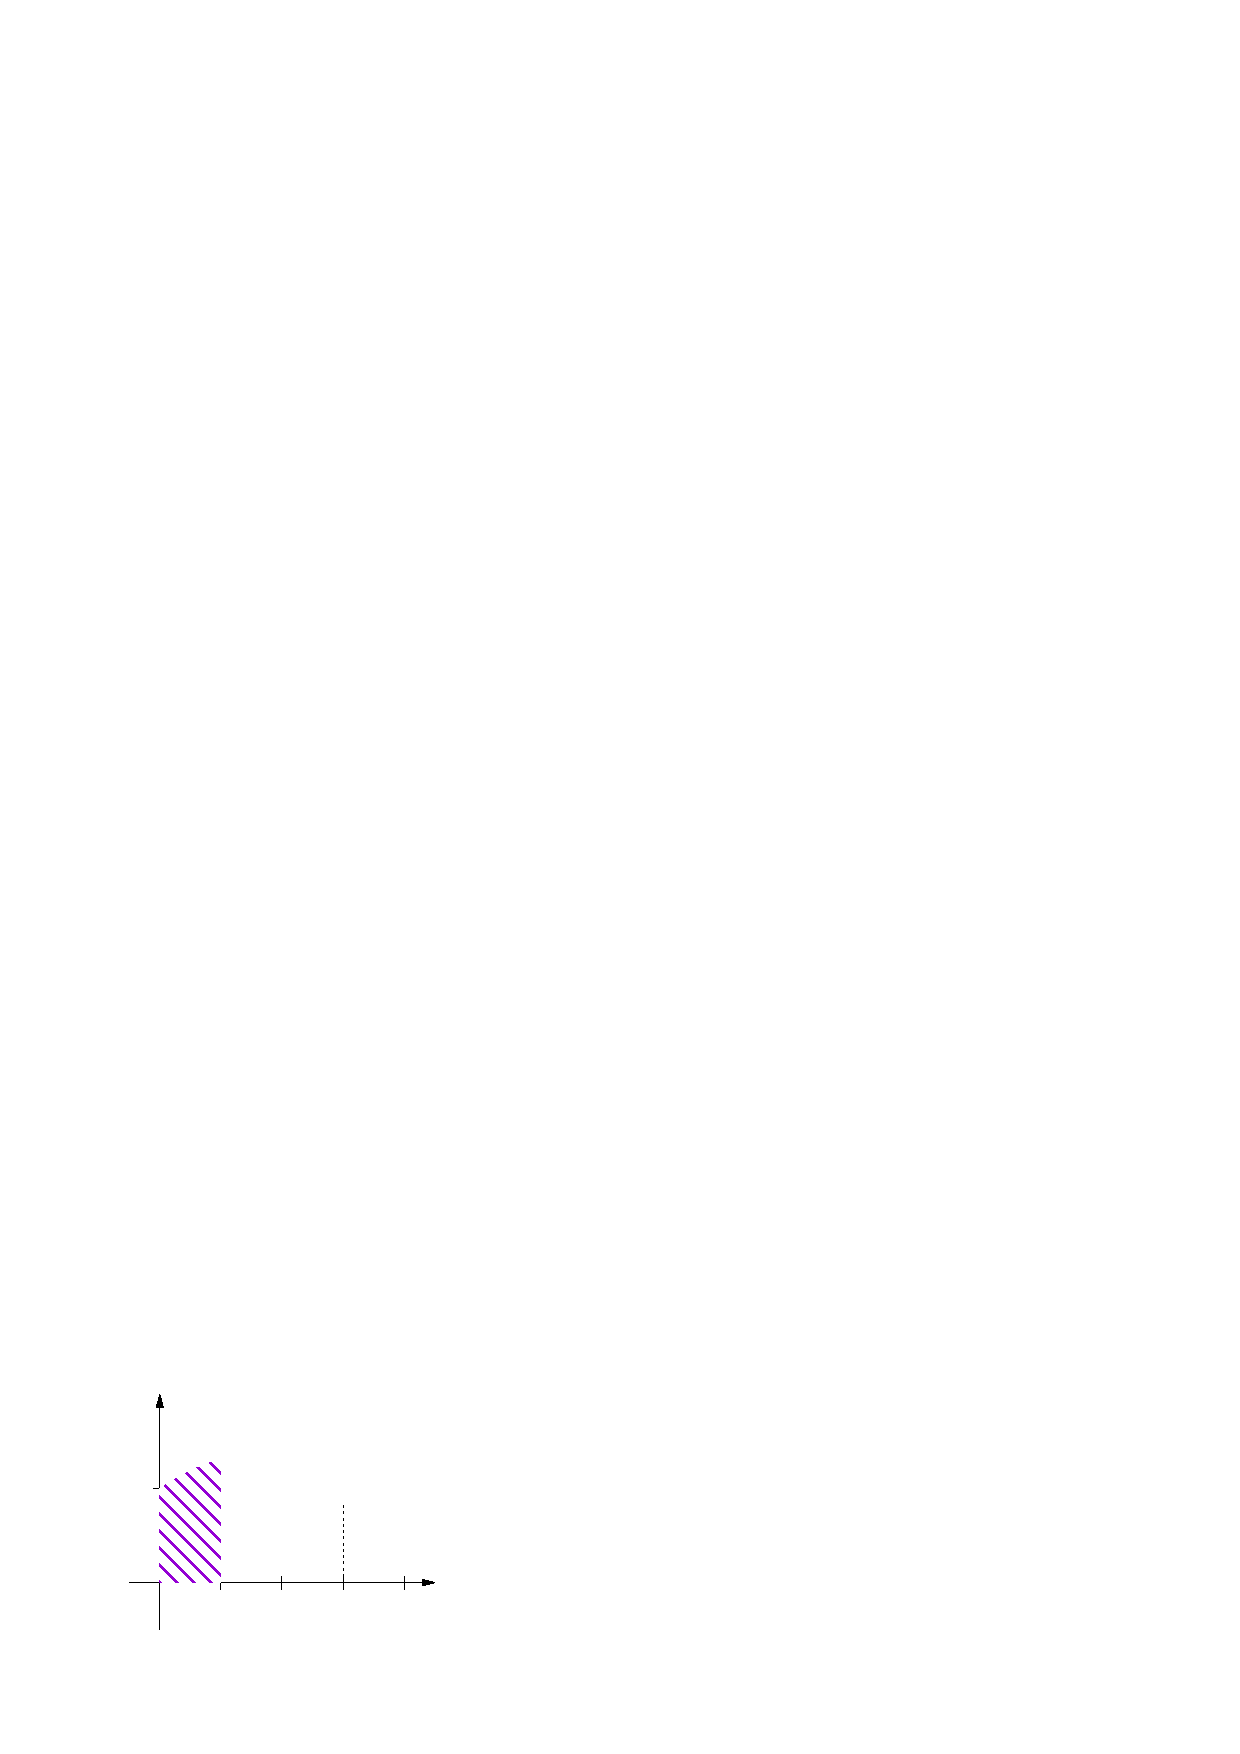
\includegraphics[width={158.40bp},height={108.00bp}]{figura_05_04}}%
    \gplfronttext
  \end{picture}%
\endgroup

    \end{minipage}
\end{figure}

\section{Transformada de \emph{Fourier} y convolución}
\begin{equation}
    \mathcal{F}\{f_1(t)*f_2(t)\}=F_1(\omega)\,F_2(\omega)
\end{equation}
Donde:
\begin{equation*}
    F_1(\omega)=\mathcal{F}\{f_1(t)\}
\end{equation*}
\begin{equation*}
    F_2(\omega)=\mathcal{F}\{f_2(t)\}
\end{equation*}

\underline{Prueba}:
\begin{equation*}
\begin{split}
    \mathcal{F}\{f_1(t)*f_2(t)\}
        &=\int_{-\infty}^{\infty}\left[
            \int_{\infty}^{\infty}f_1(\tau)f_2(t-\tau)d\tau
        \right]\,e^{-jn\omega_0\,t}\,dt\\
        &=\int_{-\infty}^{\infty}\int_{-\infty}^{\infty}
            f_1(\tau)f_2(t-\tau)\,e^{-jn\omega_0\,t}\,d\tau\,dt\\
        &=\int_{-\infty}^{\infty}\int_{-\infty}^{\infty}
            f_1(\tau)f_2(t-\tau)\,e^{-jn\omega_0\,t}\,dt\,d\tau\\
        &=\int_{-\infty}^{\infty}f_1(\tau)d\tau\,\int_{-\infty}^{\infty}
            f_2(t-\tau)\,e^{-jn\omega_0\,t}\,dt\\
\end{split}
\end{equation*}
\begin{equation*}
    u=t-\tau\rightarrow\,t=u+\tau
\end{equation*}
\begin{equation*}
    du=dt
\end{equation*}
\begin{equation*}
\begin{split}
    \mathcal{F}\{f_1(t)*f_2(t)\}
        &=\int_{-\infty}^{\infty}f_1(\tau)d\tau\,\int_{-\infty}^{\infty}
            f_2(u)\,e^{-jn\omega_0(u+\tau)}\,du\\
        &=\int_{-\infty}^{\infty}f_1(\tau)\,e^{-jn\omega_0\tau}\,d\tau\,
            \int_{-\infty}^{\infty}f_2(u)\,e^{-jn\omega_0\,u}\,du\\
        &=F_1(\omega)\,F_2(\omega)\\
\end{split}
\end{equation*}

\section{Transformada inversa de \emph{Fourier} por convolución}
\begin{equation}
    \mathcal{F}^{-1}\{F_1(\omega)\,F_2(\omega)\}=f_1(t)*f_2(t)
\end{equation}
Donde:
\begin{equation*}
    f_1(t)=\mathcal{F}^{-1}\{F_1(\omega)\}
\end{equation*}
\begin{equation*}
    f_2(t)=\mathcal{F}^{-1}\{F_2(\omega)\}
\end{equation*}

\section{Ecuaciones diferenciales ordinarias}
\begin{equation*}
    \mathcal{F}\{f'(t)\}=j\omega\,F(\omega)
\end{equation*}
\begin{equation*}
    \mathcal{F}\{f''(t)\}={(j\omega)}^2\,F(\omega)
\end{equation*}
\begin{equation*}
    \mathcal{F}\{f^{(n)}(t)\}={(j\omega)}^n\,F(\omega)
\end{equation*}


%\chapter{Transformada inversa de \emph{Laplace}}


%\chapter{Aplicaciones de la transformada de \emph{Laplace}}



\end{document}

